\documentclass[letter]{report}
\usepackage[utf8]{inputenc}
%\usepackage[applemac]{inputenc}
\usepackage[dvips]{graphics}
\usepackage[spanish]{babel}
\usepackage{fullpage}
\usepackage{euscript}
\usepackage{amsmath}
\usepackage{amssymb}
\usepackage{epsfig}
\usepackage{multicol}
\usepackage{clrscode}
\usepackage{ntheorem}
\usepackage{color}

\newcommand{\red}[1]{\textcolor{red}{#1}}
\newcommand{\blue}[1]{\textcolor{blue}{#1}}
\newcommand{\comp}{\circ}

%%%%%%%%%%%%%%%%%%%%%%%%%%%%%%%%%%%%%%%%%%%%%%%%%%%%%%%%
%%%% Algunos comandos para códigos %%%%%%%%%%%%%%%%%%%%%
%%%%%%%%%%%%%%%%%%%%%%%%%%%%%%%%%%%%%%%%%%%%%%%%%%%%%%%%
\renewcommand{\gets}{ERROR!!! }
\newcommand{\cgets}{:=}%\leftarrow}
\newcommand{\ceq}{=}
\newcommand{\cneg}{\neg}
\newcommand{\cnot}{\not}
\newcommand{\cneq}{\not=}
\newcommand{\clt}{<}
\newcommand{\cgt}{>}
\newcommand{\cleq}{\leq}
\newcommand{\cgeq}{\geq}
\newcommand{\cor}{\vee}
\newcommand{\cand}{\wedge}
\newcommand{\nil}{\const{nil} }
\renewcommand{\Do}{\bf do }
\renewcommand{\Then}{\bf then }
\renewcommand{\Else}{\bf else }
\renewcommand{\If}{{\bf if} }
\renewcommand{\While}{\bf while }

%\renewcommand{\emptyset}{o\hspace*{-1.6mm}/}
\renewcommand{\P}{\mathcal{P}}
\newcommand{\A}{\mathcal{A}}
\newcommand{\U}{\mathcal{U}}
\newcommand{\N}{\mathbb{N}}
\newcommand{\Z}{\mathbb{Z}}
\newcommand{\R}{\mathbb{R}}
\newcommand{\Q}{\mathbb{Q}}
\newcommand{\G}{\mathcal{G}}
\renewcommand{\L}{\mathcal{L}}
\newcommand{\E}{\mathcal{E}}
\newcommand{\nr}[1]{\hspace*{-0.3em}\not\hspace*{-0.3em}#1}
\newcommand{\eqr}{\sim}
\newcommand{\NP}{\emph{NP}}

\newcommand{\ssi}{\leftrightarrow}

\newcommand{\fin}{
%\vspace*{0em}\\*
\par\noindent
\rule{4cm}{0.3mm}
\par
}

%%%%%%%%%%%%%%%%%%%%%%%%%%%%%%%%%%%%%%%%%%%%%%%%%%%%%%%%%%%%%%%%%%
%%%%%%%%%%%%%%%%%%%%%%%%%%%%%%%%%%%%%%%%%%%%%%%%%%%%%%%%%%%%%%%%%%
%%%%%%%%%% Definiciones de ambientes tipo teorema %%%%%%%%%%%%%%%%
%%%%%%%%%%%%%%%%%%%%%%%%%%%%%%%%%%%%%%%%%%%%%%%%%%%%%%%%%%%%%%%%%%
%%%%%%%%%%%%%%%%%%%%%%%%%%%%%%%%%%%%%%%%%%%%%%%%%%%%%%%%%%%%%%%%%%

\newcounter{teorema}[section]
\renewcommand{\theteorema}{\thesection.\arabic{teorema}}
\newenvironment{teorema}[1][]
{\refstepcounter{teorema}{\bf Teorema \theteorema: #1}}
{\fin}

\newenvironment{lema}[1][]
{\refstepcounter{teorema}{\bf Lema \theteorema: #1}}
{\fin}

\newenvironment{corolario}[1][]
{\refstepcounter{teorema}{\bf Corolario \theteorema: #1}}
{\fin}


\newenvironment{nota}[1][]
{}
{}

\newenvironment{definicion}[1][]
{\begin{description}
\vspace*{-\topsep}
\item[Def: #1]
}
{
\vspace*{-1.2\topsep}
\end{description}}


\newenvironment{ejemplo}[1][]
{{\bf Ejemplo: #1}}
{\fin}

\newcommand{\BI}{\item[\bf B.I.]}
\newcommand{\HI}{\item[\bf H.I.]}
\newcommand{\TI}{\item[\bf T.I.]}

\newenvironment{inducciondemo}
{\begin{itemize}
\vspace*{-\topsep}
\itemsep 0pt
\itemindent 10pt
\labelwidth 20pt
\labelsep 10pt
}
{\end{itemize}
\vspace*{-\topsep}}

\newenvironment{demostracion}
{\emph{Demostración:}}
{$\Box$}



\parskip 5pt
\parindent 0pt

\begin{document}

\title{\Huge\bf Apuntes de Matem\'aticas Discretas\footnote{Apuntes escritos mientras el autor dictaba los cursos de Modelos Discretos en la Universidad de Talca (2005--2006), Matemáticas Discretas en la Universidad Católica (2007--2010), y Matemáticas Discretas en la Universidad de Chile (2011--).
Si quieres cooperar completando estros apuntes puedes hacerlo en \texttt{https://github.com/jorgeperezrojas/apuntes\_mat\_discretas}}}
\author{\LARGE Jorge P\'erez \vspace*{1em} \\ Departamento de Ciencias de la Computaci\'on  \\ Universidad de Chile \\
\vspace*{15em} \\ %
\includegraphics{logo.ps}
}
\maketitle

\pagestyle{empty}
\thispagestyle{empty}
\tableofcontents
\chapter{Fundamentos de Matemáticas Discretas}
\setcounter{chapter}{1}
\thispagestyle{empty}

\newpage
\section{Inducción}

Principio de Inducción como propiedad de los naturales y técnica para demostraciones matemáticas.
Muy usado en computación además como técnica de construcción de estructuras.

\subsection{Principios de Inducción}
Existen distintas formulaciones para el principio de inducción, veremos las más usadas.

\begin{teorema}[Principio de Buen Orden (PBO).]\label{teo:PBO}
Todo subconjunto no vacío de los naturales tiene un menor elemento\\
\[
\text{si }A\not=\emptyset \text{ y } A\subseteq \N\text{ entonces existe un }x\in A \text{ tal que } x\leq y \text{ para todo }y\in A. 
\]
\end{teorema}

Este principio no lo cumplen por ejemplo los números racionales
>Cuál es el menor elemento del conjunto $A=\{q\in \Q\;|\; q>0\}$? 
No existe un menor elemento, de hecho, supongamos que existiera tal $q_0\in A$ el menor elemento, claramente $\frac{q_0}{2}\in A$ y cumple que $0<\frac{q_0}{2}<q_0$ lo que contradice la hipótesis de que $q_0$ es el menor.
Los reales tampoco cumplen este principio (buen orden).
De hecho el PBO intuitivamente define a $\N$\footnote{En realidad, es un poco más complicado pues el PBO es definitorio para los \emph{ordinales}:
cualquier conjunto que satisface el PBO en general es equivalente a un número ordinal, pero esto escapa un poco de nuestros objetivos.}.

El anterior principio se asume para formular uno más útil:

\begin{teorema}[Principio de Inducción Simple (PIS).]
Sea $A$ un subconjunto de $\N$. Si $A$ cumple con:
\begin{enumerate}
  \item $0\in A$
  \item si $n\in A$ entonces $n+1\in A$
\end{enumerate}
entonces $A=\N$.

\begin{demostracion}
Asumimos el PBO.
Supongamos que tenemos un conjunto $A\subseteq\N$ que cumple las anteriores características y tal que $A\not=\N$.
Entonces el conjunto $B=\N-A$ cumple con $B\subseteq\N$ y con $B\not=\emptyset$.
Por el PBO, $B$ debe tener un menor elemento, digamos $b\in B$.
Es claro que $b\not=0$ (ya que $0\in A$), luego $b-1$ pertenece a $\N$ y no a $B$, por lo que se cumple $b-1\in A$.
Dado que estamos suponiendo que $A$ cumple las características del PIS entonces $b\in A$ lo que contradice el hecho de que $b$ sea el menor elemento de $B$.
La contradicción ocurre por el hecho de suponer que $A\not=\N$, luego necesariamente se cumple que $A=\N$.
\end{demostracion}
\end{teorema}

El anterior principio nos dice que cada vez que nos encontremos con un subconjunto de los naturales que contenga al $0$ y que para cada uno de sus elementos, el sucesor de él también está contenido, entonces el conjunto es exactamente el conjunto de todos los naturales.
Habitualmente a la propiedad $0\in A$ se le llama \emph{base de inducción} (BI), a la suposición de que $n\in A$ se le llama \emph{hipótesis de inducción} (HI), y a la demostración de que $n+1\in A$ se le llama \emph{tésis de inducción} (TI).

¿De qué nos sirve este principio?
Principalmente para demostrar que algunas propiedades son cumplidas por todos los números naturales.

\begin{ejemplo}
Demostraremos que el $0$ es el menor número natural usando el PIS.
Para esto definimos el siguiente conjunto:
\[
A=\{x\in\N\;|\;x\geq 0\}
\]
Si demostramos que $A=\N$ estamos demostrando que para todo elemento $x\in\N$, $x$ es mayor o igual a $0$ y que por lo tanto $0$ es el menor natural.

\begin{demostracion}
La demostración es bastante simple:
\begin{inducciondemo}
\BI Claramente $0\in A$ ya que $0\geq 0$.
\HI Supongamos que un natural $n$ fijo cumple con $n\geq 0$.
\TI Dado que $n\geq 0$ se cumple que $n+1\geq 1$ y por lo tanto $n+1\geq 0$
\end{inducciondemo}
Por PIS se sigue que $A=\N$.
\end{demostracion}
\end{ejemplo}

Generalmente el PIS se formula de una manera alternativa que hace más fácil plantear ciertos teoremas:

\begin{teorema}[Principio de Inducción Simple (segunda formulación).]
Sea $P$ una propiedad cualquiera sobre elementos de $\N$.
Si se tiene que:
\begin{enumerate}
\item $P(0)$ es verdadero ($0$ cumple la propiedad $P$)
\item $P(n)\Rightarrow P(n+1)$ (cada vez que $n$ cumple la propiedad $n+1$ también la cumple)
\end{enumerate}
Entonces todos los elementos de $\N$ cumplen la propiedad $P$.

\begin{demostracion}
La demostración es inmediata a partir de la primera formulación del PIS, sólo tome $A=\{n\in\N\;|\; P(n)$ es verdadera $\}$.
\end{demostracion}
\end{teorema}

Al igual que en la formulación anterior, a $P(0)$ se le llama BI, la suposición de $P(n)$ es HI, y la demostración de $P(n+1)$ a partir de $P(n)$ es la TI. 

\begin{ejemplo}
Demostraremos que la siguiente propiedad se cumple para todo $n$:
\[
\sum_{i=0}^{n}i=\frac{n(n+1)}{2}
\]
Para ocupar el PIS debemos definir nuestra propiedad $P$, en este caso:
\[
P(n)\;:\; \sum_{i=0}^{n}i=\frac{n(n+1)}{2}
\]

\begin{demostracion}
\begin{inducciondemo}
\BI Si $n=0$, $\sum_{i=0}^{n}=\sum_{i=0}^{0}=0$ que es igual a $\frac{n(n-1)}{2}=0$, por lo que $P(0)$ es verdadera
\HI Supongamos que $P(n)$ se cumple, o sea que $\sum_{i=0}^{n}i=\frac{n(n-1)}{2}$
\TI Queremos demostrar ahora que $P(n+1)$ se sigue cumpliendo, o sea, queremos demostrar que
\[
P(n+1)\;:\; \sum_{i=0}^{n+1}i=\frac{(n+1)((n+1)+1)}{2}
\]
es verdadero.

Ahora, es claro que
\[
\sum_{i=0}^{n+1}i=(\sum_{i=0}^{n}i)+(n+1)
\]
Por HI se cumple que
\[
\sum_{i=0}^{n+1}i=(\frac{n(n+1)}{2})+(n+1)
\]
de lo que resulta 
\[
\sum_{i=0}^{n+1}i=\frac{(n^2+n+2n+2)}{2}=\frac{n^2+3n+2}{2}=\frac{(n+1)(n+2)}{2}
\]
finalmente
\[
\sum_{i=0}^{n+1}i=\frac{(n+1)((n+1)+1)}{2}
\]
por lo que $P(n+1)$ es también verdadero.
\end{inducciondemo}
Por PIS se sigue que $P$ se cumple para todos los naturales.
\end{demostracion}
\end{ejemplo}

A veces necesitamos demostrar propiedades que se cumplen para todos los naturales exceptuando una cantidad finita de ellos.
Generalmente son propiedades de los naturales que empiezan a cumplirse desde un punto en adelante.
El PIS puede ser modificado para que la BI pueda iniciarse en cualquier número natural distinto de $0$, lo que nos importa en estos casos es que cierta propiedad se cumple para todos los naturales mayores o iguales que cierto natural fijo.
Debemos cambiar entonces la demostración de nuestra base a ese natural fijo.
El siguiente ejemplo nos muestra una aplicación de esta variación del PIS.

\begin{ejemplo}
Para todo natural $n\geq 4$ se cumple que 
\[
n!>2^n
\]
Nuestra propiedad en este caso es $P(n)\;:\;n!>2^n$.

\begin{demostracion}
\begin{inducciondemo}
\BI En este caso la base debiera iniciarse en $n=4$, entonces nos preguntamos si $P(4)$ es o no verdadero.
Ahora, $4!=1\cdot 2\cdot 3\cdot 4=24>16=2^4$, por lo que la propiedad se cumple para $4$.
\HI Supongamos que efectivamente $n!>2^n$
\TI Queremos demostrar que $(n+1)!>2^{n+1}$.
Ahora, 
\[
(n+1)!=(n+1)n!
\]
dado que estamos suponiendo que $n$ cumple la propiedad (HI) tenemos que
\[
(n+1)!=(n+1)n!>(n+1)2^n
\]
Ahora, dado que la propiedad que queremos demostrar se inicia en $n=4$ sabemos que $n+1$ es necesariamente mayor que $4$ por lo que obtenemos
\[
(n+1)!>(n+1)2^n>4\cdot 2^n>2\cdot 2^n=2^{n+1}
\]
de donde obtenemos que
\[
(n+1)!>2^{n+1}
\]
por lo que la propiedad se cumple también para $n+1$.
\end{inducciondemo}
\end{demostracion}
\end{ejemplo}

¿Cómo podemos justificar este nuevo uso del PIS a partir de la formulación con base en 0?
En vez de considerar la propiedad $P$ de arriba, pordiamos considerar la propiedad:
\[
n<4 \text{ o }n!>2^n.
\]
note que esta propiedad es verdadera (se puede demostrar usando PIS) para todos los elementos de $\N$.

Existen casos donde la inducción sirve para problemas que parecen estar muy apartados de propiedades numéricas como en el siguiente ejemplo:

\begin{ejemplo}
Queremos demostrar que cualquier tablero cuadriculado de dimensiones $2^n\times 2^n$ con $n\geq 1$ al que le falta exactamente un casillero, puede ser cubierto completamente con \emph{trominós}.
Un \emph{trominó} es una ficha como la que se muestra en la figura~\ref{fig:tromino}.

\begin{figure}[h!]
\begin{center}
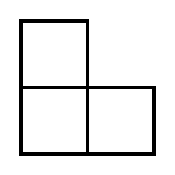
\includegraphics{eps_imgs/tromino.eps}
\end{center}
\caption{Un \emph{trominó} recto}
\label{fig:tromino}
\end{figure}

La propiedad en este caso tiene que ver con la potencia que nos da las dimensiones del tablero, o sea $P$ sería:
\begin{center}
$P(n)\;:\;$ un tablero de $2^n\times 2^n$ con un casillero menos, puede ser completamente cubierto con \emph{trominós}.
\end{center}
Lo segundo que debemos observar es que en este caso la inducción comienza en $n=1$.

\begin{demostracion}
(Demostración en clases)
\end{demostracion}
\end{ejemplo}

Al alumno de computación el anterior ejemplo debiera de inmediato parecerle, además de una demostración, un método de construcción.
Usando exactamente la misma idea de la anterior demostración se podría programar un algoritmo recursivo que, dado un tablero de dimensiones $2^n\times 2^n$ al que le falta un casillero, pueda encontrar (efectivamente) una forma de cubrirlo usando \emph{trominós}.

Existe una tercera formulación del Principio de Inducción que usa una suposición más fuerte y resulta de gran utilidad para demostrar propiedades cuando la información de que $n$ cumple la propiedad no basta para concluir que $n+1$ también la cumple.

\begin{teorema}[Principio de Inducción por Curso de Valores (PICV).]
Sea $A$ un subconjunto de $\N$.
Si para todo $n\in\N$ se cumple que 
\[
si \{x\in \N\mid x<n\} \subseteq A \text{ entonces } n\in A,
\]
entonces $A=\N$.
\end{teorema}
En este caso la parte $\{0,1,\ldots,n-1\}\subseteq A$ es la HI, y la demostración de $n\in A$ es la TI.
Un punto interesante es que \emph{pareciera} no haber una base de inducción... (¿la hay? piense en el caso $\emptyset\subseteq A$).

Al igual que con el PIS, existe una segunda formulación que hace las demostraciones más naturales.

\begin{teorema}[Principio de Inducción por Curso de Valores (segunda formulación).]
Sea $P$ una propiedad cualquiera sobre elementos de $\N$ y suponga que se cumple que:
\[
\text{si para todo }k\in\N\text{ menor que }n\text{ }P(k)\text{ es verdadero, entonces }P(n)\text{ es verdadero}.
\]
Entonces se tiene que $P$ es verdadero para todos los elementos de $\N$.
\end{teorema}

El teorema anterior nos dice que si, al suponer que cierta propiedad se cumple para todos los números naturales menores que cierto $n$ podemos concluir que $n$ también la cumple, entonces se concluye que todos los números naturales cumplen la propiedad.

\begin{ejemplo}
La sucesión de Fibonacci, es una serie de números naturales $F_0,F_1,F_2,\ldots,F_n,F_{n+1}\ldots$ que cumplen la siguiente relación de recurrencia:
\[
\begin{array}{rcl}
F_0 & = & 0 \\
F_1 & = & 1 \\
F_n & = & F_{n-1} + F_{n-2} \;\;\;\forall n\geq 2
\end{array}
\]
Demostraremos que $F_n<2^n$ para todo $n\in\N$.

\begin{demostracion}
La demostración la haremos usando el PICV.
Un punto interesante es que usaremos dos casos base, $n=0$ y $n=1$, la razón debiera quedar clara cuando finalizemos la demostración.
\begin{inducciondemo}
\BI Para $n=0$ se tiene $0<1=2^0$, para $n=1$ se tiene que $1<2=2^1$ por lo que los casos base funcionan.
\HI Supongamos que para todo $k<n$ se cumple que $F_k<2^k$.
\TI Queremos demostrar que usando HI podemos concluir que $F_n<2^n$.
Usaremos el hecho de que $F_n=F_{n-1}+F_{n-2}$, y la HI:
\[
\begin{array}{rcl}
F_n & = & F_{n-1} + F_{n-2} \\
 & \stackrel{\text{(HI)}}{<} & 2^{n-1}+2^{n-2} = \frac{3}{4}\cdot 2^n \\
 & < & 2^n \\
\end{array}
\]
\end{inducciondemo}
Por el PICV se sigue que $F_n<2^n$ para todo $n\in\N$.
\end{demostracion}
\end{ejemplo}

Un error muy frecuente entre los alumnos es hacer la inducción ``al revés''.
Inicialmente suponen que la tesis de inducción es correcta y haciendo movimientos algebráicos obtiene la hipótesis de inducción con lo que dan por terminada su demostración.
Este tipo de desarrollo se considerará siempre incorrecto ya que {\bf no se puede partir una demostración desde lo que se quiere concluir}.
Siempre se debe tener muy en claro que lo que debemos suponer es la hipótesis de inducción y a partir de ella concluir la tesis de inducción.

Más adelante en el curso veremos aplicaciones directas de los principios de inducción en el área de algoritmos computacionales, principalmente en el cálculo de la eficiencia de un algoritmo y en el establecimiento de su corrección (que el algoritmo efectivamente hace lo que dice que hace).

\subsection{Inducción Estructural}
Hemos visto distintos principios de inducción (y formulaciones de estos), todos aplicados al conjunto de los números naturales.
¿Qué tiene de especial $\N$?
Principalmente su característica de ser un conjunto que se puede construir a partir de un elemento base y un operador.
El elemento base es el $0$ y el operador es ``el sucesor''.
Intuitivamente todo natural se puede obtener a partir de sumarle $1$ a otro natural, o sea de aplicarle el operador sucesor a otro natural (excepto el $0$ que es la base).
Así una forma de definir al conjunto de los números naturales es la siguiente:
\begin{enumerate}
\itemsep 0pt
\item El $0$ es un número natural.
\item Si $n$ es un número natural entonces $n+1$ también es un número natural.
\item Todos los números naturales y sólo ellos se obtienen a partir de la aplicación de reglas 1 y 2.
\end{enumerate}
Mirando la definición debiera quedar clara la naturaleza constructiva de los números naturales y como se relaciona con el principio de inducción.
Lo que hacemos entonces para demostrar que una propiedad se cumple para todo el conjunto de los números naturales es demostrar que se cumple para su elemento base y que si suponemos que se cumple para un elemento cualquiera, el operador de construcción (sucesor en este caso) mantiene la propiedad.

¿Pueden otros conjuntos definirse de manera similar?
La respuesta es afirmativa y a estas definiciones les llamaremos \emph{definiciones inductivas}.
La implicancia más importante es que podremos usar inducción para demostrar propiedades que cumplen otros conjuntos, no sólo los naturales.
Una implicancia adicional es que podremos definir nuevos objetos (funciones, operaciones, etc) usando la definición inductiva del conjunto.

En general para definir un conjunto inductivamente necesitaremos:
\begin{enumerate}
\itemsep 0pt
\item Un conjunto (no necesariamente finito) de elementos base que se supondrá que inicialmente pertenecen al conjunto que queremos definir.
\item Un conjunto finito de reglas de construcción de nuevos elementos del conjunto a partir de elementos que ya pertenecen.
\end{enumerate}
(Omitiremos la afirmación ``Todos los elementos del conjunto y sólo ellos se obtienen a partir de la aplicación de las anteriores reglas'' pero supondremos que está implícita en la definición.)

\begin{ejemplo}
Un ejemplo muy sencillo es la definición de los números pares.
\begin{enumerate}
\itemsep 0pt
\item El $0$ es un número par.
\item Si $n$ es un número par entonces $n+2$ es un número par.
\end{enumerate}
nada muy extraño...
\end{ejemplo}

Un punto muy importante es que ningún elemento del conjunto que queremos definir se debe escapar de nuestra definición, por ejemplo la siguiente {\bf no} es una definición válida de los números pares:
\begin{enumerate}
\itemsep 0pt
\item El $0$ es un número par.
\item Si $n$ es un número par entonces $2n$ es un número par.
\end{enumerate}
¿Cuál es el problema?...

\begin{ejemplo}
Muchas veces cuando estudiamos computación nos encontramos con estructuras de datos.
Generalmente las usamos y no nos interesa demasiado formalizar ni su construcción ni las operaciones sobre ella.
En este ejemplo veremos como podemos formalizar un concepto similar al de ``lista enlazada'' muy usada en cursos de computación. 
Para simplificar la definición, supondremos que nuestras listas sólo pueden contener números naturales.

Un ejemplo de lista enlazada (de las que usaremos nosotros) es:
\[
\rightarrow 5\rightarrow 7\rightarrow 1\rightarrow 0\rightarrow 3\rightarrow 1\rightarrow 4
\]
Diremos en este caso que la lista contiene a los valores $5, 7, 1, 0, 3, 1, 4$ en ese orden (note la repetición del elemento $1$).
Una lista muy especial es la lista vacía que representaremos por
\[
\emptyset
\]
que es una lista que no contiene elemento alguno (para los que son más orientados a la programación esta lista representaría a un puntero nulo, \texttt{NULL} en C).
En este caso la lista
\[
\emptyset\rightarrow 10\rightarrow 6
\]
y la lista
\[
\rightarrow 10\rightarrow 6
\]
son exactamente iguales, ambas contienen exactamente a los elementos $10$ y $6$ en ese orden.

Con estas consideraciones no es difícil imaginar que cualquier lista que se nos ocurra se formará a partir de una lista más pequeña a la que se le ha agregado un elemento ``al final''.
La única lista que no puede ser creada entonces de esta manera es la lista vacía, que debiera ser nuestro caso base.
Así la siguiente es una definición para el conjunto $\L_\N$ de todas las listas formadas con elementos en $\N$.
\begin{enumerate}
\itemsep 0pt
\item $\emptyset$ es una lista y representa a la lista vacía ($\emptyset\in\L_\N$).
\item Si $L$ es una lista y $k$ es un natural, entonces $L\rightarrow k$ es una lista ($L\in\L_\N\Rightarrow L\rightarrow k\,\in\L_\N,\;\forall k\in\N$).
\end{enumerate}

En este caso la ``operación'' que estamos usando para crear listas es tomar una lista, y agregar una flecha ($\rightarrow$) seguida de un natural.
La ``operación flecha seguida de natural'' correspondería a sumar uno en el caso de la inducción sobre los naturales.
La anterior definición nos dice que $\emptyset$ es una lista, que $\rightarrow 4$ es una lista ya que se forma a partir de la lista vacía $\emptyset$ agregándole el natural $4$.
De la misma forma $\rightarrow 4\rightarrow 7$ es una lista ya que se forma a partir de $\rightarrow 4$ que sabemos que es una lista, al agregar el natural $7$.

Esta anterior definición además nos entrega una noción de igualdad de listas (concepto muy importante en los ejemplos posteriores):
\[
L_1\rightarrow k = L_2\rightarrow j \;\;\text{ si y sólo si }\;\; L_1=L_2 \text{ y } k=j
\]
esto quiere decir que dos listas son iguales cuando ambas han sido creadas a partir de la misma lista agregándole el mismo elmento al final.

Podemos plantear algunas propiedades que debieran cumplir todas las listas y demostrarlas por inducción estructural, es decir usando inducción en el dominio constructible de las listas.
Demostraremos a modo de ejemplo que toda lista tiene exactamente la misma cantidad de elementos que de flechas ($\rightarrow$).

\begin{demostracion}
En este caso la propiedad $P$ es sobre el conjunto $\L_\N$ de todas las listas con elementos naturales y se define por:
\[
P(L)\;:\;L\text{ tiene el mismo número de flechas que de elementos.}
\]
\begin{inducciondemo}
\BI El caso base es la lista vacía, ella tiene ningún elemento y ninguna flecha por lo que cumple con la propiedad, o sea $P(\emptyset)$ es verdadero.
\HI Supongamos que una lista cualquiera $L$ tiene exactamente tantos elementos como flechas, o sea que $P(L)$ es verdadero.
\TI Queremos demostrar que $P(L\rightarrow k)$ es verdadero, o sea que la lista $L\rightarrow k$ con $k\in\N$, también cumple la propiedad.
%\footnote{note que en este caso decir $L\rightarrow  k$ es equivalente a decir $n+1$ en el PIS.}
Es claro que la lista $L\rightarrow k$ tiene exactamente una flecha más y exactamente un elemento más que $L$.
Dado que estamos suponiendo que $P(L)$ se cumple (HI), concluimos que $L\rightarrow k$ tiene exactamente el mismo número de flechas que de elementos, por lo que $P(L\rightarrow k)$ también se cumple.
\end{inducciondemo}
Por inducción estructural se sigue que todas las listas en $\L_\N$ tienen la misma cantidad de flechas que de elementos.
\end{demostracion}
\end{ejemplo}

Algo muy interesante de las definiciones inductivas de conjuntos, es la posibilidad de aprovechar el carácter de constructivo para definir operadores o funciones sobre los elementos.
Cuando estas definiciones se hacen en los naturales generalmente se les llama ``definiciones recursivas'', por ejemplo, la definición del operador factorial ($!$) sobre $\N$ se hace de la siguiente manera:
\begin{enumerate}
\itemsep 0pt
\item $0!=1$.
\item $(n+1)!=(n+1)\cdot n!$.
\end{enumerate}
Aquí se está aprovechando la forma de construcción de los naturales para definir de manera elegante un operador sobre todos los naturales.
Se define el caso base ($0$) y se explicita como operar el siguiente elemento que ha sido creado por inducción (sucesor) suponiendo que el operador ya está definido sobre los demás elementos del conjunto.

De manera similar podemos definir funciones y operadores sobre otros conjuntos creados por inducción estructural, el siguiente ejemplo muestra definiciones para el dominio de las listas.

\begin{ejemplo}
La función $|\cdot|:\L_\N\rightarrow\N$ (que a la lista $L$ se aplica como $|L|$) toma una lista como argumento y entrega el entero correspondiente a la cantidad de elementos de la lista, es decir el largo de la lista.
Queremos definir la función $|\cdot|$ inductivamente sobre el dominio constructible de las listas $\L_\N$.
Primero debemos definir el caso base, o sea el resultado de $|\emptyset|$.
Naturalmente el resultado debiera ser $0$, luego la primera parte de nuestra definición debiera ser:
\[
|\emptyset| = 0
\]
Queremos definir ahora que pasa con el largo de una lista que ha sido creada a partir de otra anterior.
La única forma que conocemos de crear una nueva lista es agregarle un elemento al final de la primera, es claro que el largo de la nueva lista será el largo de la primera más 1, luego la segunda parte de nuestra definición debiera ser:
\[
|L\rightarrow k|=|L|+1
\]

Finalmente la definición completa de la función $|\cdot|$ que toma una lista y entrega su largo resulta:
\begin{enumerate}
\itemsep 0pt
\item $|\emptyset|=0$
\item $|L\rightarrow k|=|L|+1$
\end{enumerate}
con $L$ lista y $k\in\N$.
\end{ejemplo}

La noción de largo de una lista ya la habíamos usamos, de manera intuitiva, cuando demostramos que toda lista tiene exactamente la misma cantidad de flechas que de elementos.
De la misma forma como definimos $|\cdot|$ podríamos definir la función $\stackrel{\rightarrow}{|\cdot|}:\L_\N\rightarrow\N$ que toma una lista cualquiera y entrega como resultado la cantidad de flechas de la lista.
Así la demostración de que toda lista tiene exactamente la misma cantidad de flechas que de elementos puede formularse como:
\[
\forall L\in\L_\N\;\;\;\stackrel{\rightarrow}{|L|}=|L|
\]
Más adelante veremos propiedades de las listas que tienen que ver con funciones y operadores definidos para ellas y que pueden demostrarse por inducción.

\begin{ejemplo}
La función $\text{sum}:\L_\N\rightarrow\N$ toma una lista como argumento y entrega el entero correspondiente a la suma de todos los elementos de la lista.
Por ejemplo
\[
\text{sum}(\rightarrow 5\rightarrow 7\rightarrow 1\rightarrow 0\rightarrow 3\rightarrow 1\rightarrow 4)=21
\]
Definiremos la función $\text{sum}$ de forma inductiva sobre el dominio constructible de las listas.
Primero debemos definir el caso base, o sea el resultado de aplicar $\text{sum}$ a la lista vacía.
Naturalmente el resultado debiera ser $0$, ya que la lista no contiene elemento alguno.
Ahora tenemos que arreglárnosla para definir $\text{sum}$ para una lista cualquiera construida a partir de una lista anterior.
Es claro que sumar todos los elementos de una lista es equivalente a sumar todos los elementos del tramo inicial de la lista y al resultado sumarle el último elemento.
Finalmente la definición completa de la función $\text{sum}$ que toma una lista y entrega la suma de sus valores resulta:
\begin{enumerate}
\itemsep 0pt
\item $\text{sum}(\emptyset)=0$
\item $\text{sum}(L\rightarrow k)=\text{sum}(L)+k$
\end{enumerate}
con $L$ lista y $k\in\N$.

Usando esta definición podemos calcular la suma de la lista $\rightarrow 2\rightarrow 3\rightarrow 5$ de la siguiente manera:
\[
\begin{array}{rcl}
\text{sum}(\rightarrow 2\rightarrow 3\rightarrow 5) & = & \text{sum}(\rightarrow 2\rightarrow 3) + 5 \\
& = & \text{sum}(\rightarrow 2) + 3 + 5\\
& = & \text{sum}(\emptyset) + 2 + 3 + 5\\
& = & 0 + 2+ 3 + 5\\
& = & 10
\end{array}
\]
\end{ejemplo}

\begin{ejemplo}
Definiremos la función $\max:\L_\N\rightarrow\N\cup\{-1\}$ de una lista, que entrega el valor del elemento más grande en la lista.
Por convención, supondremos que el elemento máximo de la lista vacía es $-1$ (¿Por qué tiene sentido esta suposición?).
Nuestra definición entonces resulta:
\begin{enumerate}
\itemsep 0pt
\item $\max(\emptyset)=-1$
\item $
\max(L\rightarrow k)=\left\{
\begin{array}{cl}
\max(L) & \text{si }\max(L)\geq k \\
k & \text{si }k>\max(L)
\end{array}\right.
$
\end{enumerate}
Como ejercicio se puede hacer algo similar al ejemplo anterior para calcular $\max(\rightarrow 4\rightarrow 1\rightarrow 7\rightarrow 3)$.
\end{ejemplo}

\begin{ejemplo}
En este ejemplo veremos la definición de la función $Head:\L_\N\rightarrow\N$ que dada una lista entrega el primer elemento contenido en ella (la ``cabeza'' de la lista).
Una cosa interesante de esta función es que no está definida para todas las listas de naturales, de hecho la lista vacía no tiene elemento alguno, por lo tanto no tiene un primer elemento.
La función estará entonces, parcialmente definida por inducción.
\begin{enumerate}
\itemsep 0pt
\item $Head(\rightarrow k)=k$
\item Si $L$ es una lista no vacía $(L\not=\emptyset)$, $Head(L\rightarrow k)=Head(L)$.
\end{enumerate}
Se debe notar que para esta definición existe una infinidad de casos base (tantos como elementos de $\N$).
\end{ejemplo}

Todos los anteriores ejemplos tienen que ver con funciones sobre listas que entregan un elemento natural, en la siguiente definición veremos un operador sobre listas, es decir, una función que toma una lista y entrega como resultado otra lista.

\begin{ejemplo}
Queremos definir el operador $Suf:\L_\N\rightarrow\L_\N$ (operador \emph{sufijo}) que toma una lista y entrega la lista que resulta de ella al sacar el primer elemento.
La definición entonces resulta:
\begin{enumerate}
\itemsep 0pt
\item $Suf(\rightarrow k)=\emptyset$
\item Si $L$ es una lista no vacía, $Suf(L\rightarrow k)=Suf(L)\rightarrow k$.
\end{enumerate}
Note que en este caso el operador tampoco está definido para la lista vacía.
\end{ejemplo}

Ahora con las varias funciones definidas podemos plantear muchas propiedades acerca de listas y demostrarlas usando inducción estructural.

\begin{teorema}
Las siguientes son propiedades de las listas:
\begin{enumerate}
\itemsep 0pt
\item $\forall L\in\L_\N$ se cumple $\text{sum}(L)\geq 0$.
\item $\forall L\in\L_\N$ se cumple $\max(L)\leq\text{sum}(L)$. \label{listprop1}
%\item $\forall L\in\L_\N$, $L\not=\emptyset$ se cumple que $L=\rightarrow Head(L)Suf(L)$.
\item $\forall L\in\L_\N$, $\text{sum}(L)=Head(L)+\text{sum}(Suf(L))$.
\item $\forall L_1,L_2\in\L_\N$, $L_1,L_2\not=\emptyset$, se cumple $L_1=L_2$ si y sólo si $Suf(L_1)=Suf(L_2)$ y $\text{sum}(L_1)=\text{sum}(L_2)$. \label{listprop2}
\item Muchas otras propiedades que se pueden plantear...
\end{enumerate}
\begin{demostracion}
A modo de ejemplo demostraremos sólo las propiedades~\ref{listprop1} y~\ref{listprop2}, las demás se proponen como ejercicios.
\begin{enumerate}
	\setcounter{enumi}{1}
	\item Por inducción estructural en $\L_\N$:
	\begin{inducciondemo}
		\BI $\max(\emptyset)=-1\leq 0=\text{sum}(\emptyset)$, por lo que $\emptyset$ cumple la propiedad.
		\HI Supongamos que para toda lista $L$ se cumple que $\max(L)\leq\text{sum}(L)$.
		\TI Queremos demostrar que $L\rightarrow k$ con $k\in \N$ también cumple, o sea, $\max(L\rightarrow k)\leq\text{sum}(L\rightarrow k)$.
		
		La definición de la función $\max$ nos habla de dos casos
		\[
		\max(L\rightarrow k)=\left\{
		\begin{array}{cl}
		\max(L) & \text{si }\max(L)\geq k \\
		k & \text{si }k>\max(L)
		\end{array}\right.
		\]
		seguiremos la demostración para cada uno de estos casos:
		
		Si $\max(L\rightarrow k)=\max(L)$ tenemos que
		  \[
		  \begin{array}{rcl}
		  \max(L\rightarrow k) & = & \max(L) \\
		  & \leq & \max(L) + k \;\;\; \text{(ya que }k\in\N\text{)}\\
		  & \stackrel{\text{HI}}{\leq}& \text{sum}(L) + k \; =\; \text{sum}(L\rightarrow k)
		  \end{array}
		  \]
		
		Si $\max(L\rightarrow k)=k$ tenemos que
		  \[
		  \max(L\rightarrow k)\;\;=\;\;k\;\stackrel{\text{(1.)}}{\leq}\;\;\text{sum}(L) + k\;\;=\;\;\text{sum}(L\rightarrow k)
		  \]
		
		En cualquier caso se cumple que $\max(L\rightarrow k)\leq\text{sum}(L\rightarrow k)$, luego por inducción estructural se sigue que la propiedad se cumple para todas las listas.
	\end{inducciondemo}
	\setcounter{enumi}{3}
	\item Primero, es claro que si $L_1=L_2$ entonces se cumple que $Suf(L_1)=Suf(L_2)$ y que $\text{sum}(L_1)=\text{sum}(L_2)$ ya que ambas son funciones y la igualdad está bien definida.
	El punto complicado es demostrar la implicación inversa: si $Suf(L_1)=Suf(L_2)$ y $\text{sum}(L_1)=\text{sum}(L_2)$ entonces $L_1=L_2$.
	Demostraremos esto útlimo por inducción estructural en $\L_\N$:
	\begin{inducciondemo}
	  \BI En este caso no podemos tomar $\emptyset$ como base ya que $Suf$ no está definido para $\emptyset$.
	  Tomaremos como base entonces listas con un elemento.
	  Sean $L_1=\rightarrow k$ y $L_2=\rightarrow j$ dos listas, dado que $\text{sum}(L_1)=\text{sum}(L_2)$ tenemos que $\text{sum}(\rightarrow k)=\text{sum}(\rightarrow j)$ y por lo tanto $k=j$ por lo que las listas $L_1$ y $L_2$ son iguales.
	  \HI Supongamos que si $Suf(L_1)=Suf(L_2)$ y $\text{sum}(L_1)=\text{sum}(L_2)$ entonces $L_1=L_2$ para cualquier par de listas $L_1$, $L_2$.
	  \TI Sean ahora dos listas $L_1\rightarrow k$ y $L_2\rightarrow j$, tales que
	  \[
	  \begin{array}{l}
	  Suf(L_1\rightarrow k)=Suf(L_2\rightarrow j) \;\;\;\text{ y} \\
	  \text{sum}(L_1\rightarrow k)=\text{sum}(L_2\rightarrow j)\text{.}
	  \end{array}
	  \]
	  Por la definición de $Suf$ y $\text{sum}$ obtenemos 
	  \[
	  \begin{array}{l}
	  Suf(L_1)\rightarrow k = Suf(L_2)\rightarrow j \\
	  \text{sum}(L_1)+k=\text{sum}(L_2)+j
	  \end{array}
	  \]
	  de la primera de estas ecuaciones y usando la definición de igualdad de listas obtenemos el hecho de que necesariamente $Suf(L_1)=Suf(L_2)$ y que $k=j$.
	  Usando este último resultado en la segunda ecuación obtenemos que $\text{sum}(L_1)=\text{sum}(L_2)$.
	  Tenemos entonces que $Suf(L_1)=Suf(L_2)$, $\text{sum}(L_1)=\text{sum}(L_2)$, y por la HI resulta que $L_1=L_2$ y dado que $k=j$ obtenemos que $L_1\rightarrow k=L_2\rightarrow j$.
	\end{inducciondemo}
	%Por inducción estructural sobre $\L_\N$ se cumple que para todo par de listas no vacías la propiedad se cumple.
\end{enumerate}
\end{demostracion}
\end{teorema}

Los ejemplos anteriores tienen que ver con la construcción de listas.
Un punto que se debe notar es que cada lista se construye a partir de una única lista anterior, al igual que en el PIS en donde el paso inductivo tiene que ver exclusivamente con el antecesor de un natural.
De manera similar al PICV podemos definir conjuntos inductivamente, usando para la construcción de un elemento particular uno o más de los elementos anteriores (anteriormente construidos).
Luego para definir propiedades y demostrar teoremas sobre el nuevo conjunto definido tendremos que usar una estrategia más similar al PICV que al PIS.
En el siguiente ejemplo veremos como se aplican estas ideas.

\begin{ejemplo}
Queremos definir el conjunto $\E_{\N}$ de todas las expresiones aritméticas que se pueden formar con números naturales, el símbolo \texttt{+}, el símbolo \texttt{*} y los símbolos de paréntesis \texttt{(} y \texttt{)}.
	Por ejemplo, los siguientes son elementos de $\E_{\N}$ (son expresiones aritméticas)
	\begin{center}
	\texttt{( $4$ + $5$ * $7$ ) * $9$} \\
	\texttt{$12$ + $2$ + $3$ + $2$ * $11$} \\
	\texttt{( $143$ + $9$ )} \\
	\texttt{$3$}
	\end{center}
	Note que no nos interesa el \emph{valor} de la expresión, sólo nos interesa la forma en que esta ``se ve''.
	El conjunto $\E_\N$ puede definirse inductivamente usando una definición inductiva por curso de valores, es decir, definiendo un elemento posiblemente a partir de varios de los elementos anteriores.
	Una expresión vacía no tiene sentido, así que nuestro caso base (la expresión más pequeña) sería un natural cualquiera, luego:
	\begin{center}
	Si $k$ es un natural, entonces $k$ es una expresión ($k\in\N\;\Rightarrow\;k\in\E_\N$).
	\end{center}
	No es difícil notar que otra manera de crear una expresión es ``sumando'' dos expresiones, o más formalmente, poniéndole un símbolo \texttt{+} entre las expresiones, así uno de los pasos inductivos será:
	\begin{center}
	Si $E_1$ y $E_2$ son expresiones, entonces \texttt{$E_1$ + $E_2$} es una expresión (\texttt{$E_1,E_2\in\E_\N\;\Rightarrow\;E_1$ + $E_2\in\E_\N$}).
	\end{center}
	Necesitamos completar la definición inductiva de las expresiones aritméticas, especificando como crear expresiones usando \texttt{*} y \texttt{()}.
	Finalmente nuestra definición resulta:
	\begin{enumerate}
	\itemsep 0pt
	\item Si $k$ es un natural, entonces $k$ es una expresión ($k\in\N\;\Rightarrow\;k\in\E_\N$).
	\item	Si $E_1$ y $E_2$ son expresiones, entonces \texttt{$E_1$ + $E_2$} es una expresión (\texttt{$E_1,E_2\in\E_\N\;\Rightarrow\;E_1$ + $E_2\in\E_\N$}).
	\item	Si $E_1$ y $E_2$ son expresiones, entonces \texttt{$E_1$ * $E_2$} es una expresión (\texttt{$E_1,E_2\in\E_\N\;\Rightarrow\;E_1$ * $E_2\in\E_\N$}).
	\item	Si $E$ es una expresión, entonces \texttt{($E$)} es una expresión (\texttt{$E\in\E_\N\;\Rightarrow\;$ ($E$) $\in\E_\N$}).
	\end{enumerate}
	
	En este caso los ``operadores'' usados para crear las expresiones son unir dos expresiones mediante un \texttt{+} o mediante un \texttt{*} y cerrar una expresión entre \texttt{()}.
	\end{ejemplo}
	
	\begin{ejemplo}
	La siguiente es una definición inductiva sobre $\E_\N$ del operador $\#_L:\E_\N\rightarrow\N$ que dada una expresión, entrega la cantidad de paréntesis izquierdos de ella.
	\begin{enumerate}
	\itemsep 0pt
		\item $\#_L(k)=0$ para todo $k\in\N$.
		\item $\#_L(E_1$\texttt{ + }$E_2)=\#_L(E_1)+\#_L(E_2)$ \hspace*{1em}para todas $E_1,E_2\in\E_\N$.
		\item $\#_L(E_1$\texttt{ * }$E_2)=\#_L(E_1)+\#_L(E_2)$ \hspace*{1em}para todas $E_1,E_2\in\E_\N$.
		\item $\#_L($\texttt{($E$)}$)=1+\#_L(E)$ \hspace*{1em}para toda $E\in\E_\N$.
	\end{enumerate}
	En esta definición se debe tener muchísimo cuidado en comprender la diferencia entre \texttt{+} y $+$.
	El primero es el símbolo utilizado para la creación de las operaciones aritméticas (es sólo un símbolo, no debiera significar nada...), el segundo representa a la suma de números naturales y tiene el sentido habitual.
	
	De manera similar se puede definir el operador $\#_R:\E_\N\rightarrow\N$ que cuenta la cantidad de paréntesis derechos de una expresión aritmética:
	\begin{enumerate}
	\itemsep 0pt
		\item $\#_R(k)=0$ para todo $k\in\N$.
		\item $\#_R(E_1$\texttt{ + }$E_2)=\#_R(E_1)+\#_R(E_2)$ \hspace*{1em}para todas $E_1,E_2\in\E_\N$.
		\item $\#_R(E_1$\texttt{ * }$E_2)=\#_R(E_1)+\#_R(E_2)$ \hspace*{1em}para todas $E_1,E_2\in\E_\N$.
		\item $\#_R($\texttt{($E$)}$)=1+\#_R(E)$ \hspace*{1em}para toda $E\in\E_\N$.
	\end{enumerate}
	\end{ejemplo}
	
	El siguiente resulta ser un teorema muy simple acerca de las expresiones aritméticas.
	
	\begin{teorema}
	Toda expresión aritmética tiene exactamente la misma cantidad de paréntesis derechos que izquierdos, o sea:
	\[
	\forall E\in\E_\N\;\;\;\;\; \#_L(E)=\#_R(E).
	\]
	\begin{demostracion}
	La demostración resulta inmediata a partir de las definiciones inductivas de ambos operadores, sus resultados aplicados a las mismas expresiones son exactamente los mismos.
	De todas maneras y sólo por completitud se presenta la demostración por inducción estructural en la construcción de $\E_\N$:
	\begin{inducciondemo}
	  \BI Si la expresión es un natural $k\in\N$ por definición tenemos que $\#_L(k)=0=\#_R(k)$.
	  \HI Supongamos que $E_1$ y $E_2$ son expresiones que cumplen con $\#_L(E_1)=\#_R(E_1)$ y $\#_L(E_2)=\#_R(E_2)$
	  \TI Tenemos tres casos para nuestra tesis que aparecen de la construcción inductiva de $\E_\N$:
	  \begin{itemize}
	    \item \texttt{$E_1$ + $E_2$}: Tenemos que \texttt{$\#_L(E_1$ + $E_2)$}$=\#_L(E_1) + \#_L(E_2)\stackrel{HI}{=}\#_R(E_1) + \#_R(E_2)=$\texttt{$\#_R(E_1$ + $E_2)$}.
	    \item \texttt{$E_1$ * $E_2$}: Igual al caso anterior.
	    \item \texttt{($E_1$)}: Tenemos que \texttt{$\#_L($($E_1$)$)=1+\#_L(E_1)\stackrel{HI}{=}1+\#_R(E_1)=\#_R($($E_1$)$)$}.
	  \end{itemize}
	\end{inducciondemo}
	En cada caso la propiedad se cumple para los pasos inductivos de la construcción de $\E_\N$.
	\end{demostracion}
	\end{teorema}
	  
A pesar de que los únicos ejemplos que usamos para inducción estructural fueron las listas enlazadas y las expresiones aritméticas, existen muchos otros dominios constructibles que pueden definirse de manera similar.
En lo que sigue del curso, varias veces nos encontraremos con definiciones inductivas de objetos (conjuntos) y con definiciones de funciones y operadores sobre ellos.
El alumno debe practicar planteándose dominios aptos para ser construidos en forma inductiva, plantear funciones sobre sus elementos y demostrar algunos teoremas que puedan surgir en el dominio.


\newpage



\section{L\'ogica Proposicional}

\subsection{Sintaxis de la L\'ogica Proposicional}

Usaremos variables proposicionales para indicar proposiciones {\em completas} e {\em indivisibles}.
En general llamaremos $P$ al conjunto de variables proposicionales, y, por ejemplo,
$p$, $q$, $r$, socrates\_es\_hombre, a las variables mismas.

\begin{definicion}
Sea $P$ un conjunto de variables proposicionales.
El conjunto de todas las {\em f\'ormulas} de l\'ogica proposicional sobre $P$,
denotado por $L(P)$, se define inductivamente por:
\begin{itemize}
\item Si $p\in P$, entonces $p$ es una f\'ormula en $L(P)$.
\item Si $\varphi\in L(P)$, entonces $(\neg \varphi)$ es una f\'ormula en $L(P)$
\item Si $\varphi,\psi\in L(P)$, entonces $(\varphi \wedge \psi)$,
$(\varphi \vee \psi)$, $(\varphi \to \psi)$, y $(\varphi \ssi \psi)$ son f\'ormulas en $L(P)$
\end{itemize}
\end{definicion}

\subsection{Sem\'antica de la L\'ogica Proposicional}

>Cu\'ando una f\'ormula es verdadera? depende del {\em mundo} en el que la estamos interpretando.
Un mundo particular le dar\'a una interpretaci\'on a cada variable proposicional, le dar\'a un
valor {\em verdadero} o {\em falso} a cada variable.

Una {\em valuaci\'on} (o {\em asignaci\'on de verdad}) para las variables de
$P$ es una funci\'on, $\sigma:P\to \{0,1\}$.

\begin{definicion}
Sea $P$ un conjunto de variables proposicionales y $\sigma$ una asignaci\'on de verdad para $P$.
Dada una f\'ormula $\varphi$ en $L(P)$, se definimos la funci\'on $\hat\sigma:L(P)\to \{0,1\}$, 
por inducci\'on como sigue:
\begin{itemize}
\item Si $p\in P$ entonces $\hat\sigma(p)=\sigma(p)$.
\item \[\hat\sigma(\, (\neg \varphi)\, )= 
      \left\{ 
      \begin{array}{cl}
      1 & \text{si }\hat\sigma(\varphi)=0, \\
      0 & \text{si }\hat\sigma(\varphi)=1. \\
      \end{array}
      \right.
\]
\item
\[\hat\sigma(\, (\varphi \vee \psi)\, )= 
      \left\{ 
      \begin{array}{cl}
      1 & \text{si }\hat\sigma(\varphi)=1\text{ o }\hat\sigma(\psi)=1, \\
      0 & \text{si }\hat\sigma(\varphi)=0\text{ y }\hat\sigma(\psi)=0. \\
      \end{array}
      \right.
\]

\[\hat\sigma(\, (\varphi \wedge \psi)\, )= 
      \left\{ 
      \begin{array}{cl}
      1 & \text{si }\hat\sigma(\varphi)=1\text{ y }\hat\sigma(\psi)=1, \\
      0 & \text{si }\hat\sigma(\varphi)=0\text{ o }\hat\sigma(\psi)=0. \\
      \end{array}
      \right.
\]

\[\hat\sigma(\, (\varphi \to \psi)\, )= 
      \left\{ 
      \begin{array}{cl}
      1 & \text{si }\hat\sigma(\varphi)=0\text{ o }\hat\sigma(\psi)=1, \\
      0 & \text{si }\hat\sigma(\varphi)=1\text{ y }\hat\sigma(\psi)=0. \\
      \end{array}
      \right.
\]

\[\hat\sigma(\, (\varphi \ssi \psi)\, )= 
      \left\{ 
      \begin{array}{cl}
      1 & \text{si }\hat\sigma(\varphi)=\hat\sigma(\psi), \\
      0 & \text{si }\hat\sigma(\varphi)\neq\hat\sigma(\psi). \\
      \end{array}
      \right.
\]
\end{itemize}
Diremos que $\hat\sigma(\varphi)$ es la {\em evaluaci\'on} de $\varphi$ dada la 
asignaci\'on $\sigma$.
\end{definicion}

De ahora en adelante llamaremos simplemente $\sigma$ a $\hat\sigma$, y denotaremos a la
a la evaluaci\'on de la f\'ormula $\varphi$ dada la asignaci\'on $\sigma$, simplmente como $\sigma(\varphi)$.

\begin{definicion}
Las f\'ormulas $\varphi,\psi\in L(P)$ son {\em l\'ogicamente equivalentes}, si para toda asignaci\'on de verdad $\sigma$ se tiene
que $\sigma(\varphi)=\sigma(\psi)$. 
Denotaremos por $\equiv$ la equivalencia l\'ogica, as\'{i}, si $\varphi$ y $\psi$ son l\'ogicamente equivalentes, escribiremos
$\varphi\equiv \psi$.
\end{definicion}

\begin{ejemplo}
Demostraremos que las f\'ormulas $(p\to q)$ y $((\neg p) \vee q)$ son l\'ogicamente equivalentes.
Dado que ambas f\'ormulas tienen s\'olo dos variables proposicionales, la cantidad de valuaciones $\sigma:\{p,q\}\to \{0,1\}$
son 4. Podemos probarlas todas en una tabla como la que sigue:

\begin{center}
\begin{tabular}{lcccc} %\cline{2-5} 
& ~$p$~ & ~$q$~ & ~$(p\to q)$~ & ~$((\neg p) \vee q)$~ \\ \cline{2-5} 
$\sigma_1$: & 0 & 0 & 1 & 1\\ %\cline{2-5}
$\sigma_2$: & 0 & 1 & 1 & 1\\ %\cline{2-5}
$\sigma_3$: & 1 & 0 & 0 & 0\\ %\cline{2-5}
$\sigma_4$: & 1 & 1 & 1 & 1\\ %\cline{2-5}
\end{tabular}
\end{center}

Cada fila de la anterior tabla corresponde a una asignaci\'on de verdad diferente, las dos primeras columnas
corresponden a las asignaciones a las variables, y las dos siguientes al valor de verdad asignado a cada f\'ormula.
En este caso, ambas f\'ormulas tienen exactamente el mismo valor de verdad para cada posible asignaci\'on por lo tanto
son equivalentes. Concluimos entonces que $(p\to q)\equiv ((\neg p)\vee q)$.
\end{ejemplo}

El anterior es un ejemplo del uso de {\em Tablas de Verdad}, que son tablas en las que las filas representan
todas las posibles valuaciones para un conjunto de variables proposicionales, 
y las columnas, etiquetadas con una f\'ormula particular,
representan los distintos valores de verdad de la f\'ormula en cada valuaci\'on.
Note que dos f\'ormulas son l\'ogicamente equivalentes, si y solo si, su respectivas columnas en una tabla de verdad
contienen exactamente la misma secuencia de valores.
Las tablas tambi\'en nos permiten establecer algunas propiedades de conteo.
Suponga que $P=\{p_1,p_2,\ldots, p_n\}$, >cu\'antas f\'ormulas no equivalentes hay en $L(P)$? 
Calcule este n\'umero y contrastelo con la cantidad de f\'ormulas distintas en $L(P)$.

Se puede demostrar que el reemplazo de sub-f\'ormulas equivalentes en una f\'ormula, no
altera el valor de verdad de la f\'ormula original.
M\'as formalmente, sea $\varphi$ una f\'ormula que contiene a $\psi$ como sub-f\'ormula, y sea
$\psi'$ una f\'ormula tal que $\psi\equiv \psi'$. 
Si $\varphi'$ es la f\'ormula obtenida de $\varphi$ reemplazando $\psi$ por $\psi'$, entonces $\varphi\equiv \varphi'$.
(Haga la demostraci\'on de esta \'ultima propiedad por inducci\'on estructural. Para
esto primero deber\'a definir inductivamente el concepto de sub-f\'ormula y formalizar
lo que significa reemplazar una sub-f\'ormula por otra).

Las siguientes son algunas equivalencias \'utiles (demuestre que se cumplen):
\begin{enumerate}
\item $(\varphi \vee \psi) \equiv (\psi \vee \varphi)$
\item $(\varphi \wedge \psi) \equiv (\psi \wedge \varphi)$
\item $(\varphi \vee (\psi \vee \chi)) \equiv ((\varphi \vee \psi) \vee \chi)$
\item $(\varphi \wedge (\psi \wedge \chi)) \equiv ((\varphi \wedge \psi) \wedge \chi)$
\item $(\varphi \vee (\psi \wedge \chi)) \equiv ((\varphi \vee \psi) \wedge (\varphi \vee \chi))$
\item $(\varphi \wedge (\psi \vee \chi)) \equiv ((\varphi \wedge \psi) \vee (\varphi \wedge \chi))$
\item $(\neg (\varphi \wedge \psi))\equiv ((\neg \varphi) \vee (\neg \psi))$
\item $(\neg (\varphi \vee \psi))\equiv ((\neg \varphi) \wedge (\neg \psi))$
\item $(\neg(\neg \varphi))\equiv \varphi$
\end{enumerate}

Las reglas 3 y 4, nos permiten evitar par\'entesis cuando consideramos secuencias de f\'ormulas operadas
usando $\vee$ y $\wedge$, respectivamente. 
De ahora en adelante escribiremos simplemente $\varphi_1 \vee \varphi_2 \vee \varphi_3$ (sin usar
par\'entesis de asociaci\'on).
Adicionalmente escribiremos 
\[
\bigvee_{i=1}^{n}\varphi_i = \varphi_1 \vee \varphi_2 \vee \cdots \vee \varphi_n.
\] Similarmente lo haremos con $\wedge$.

\begin{definicion}
Una f\'ormula $\varphi\in L(P)$ es:
\begin{itemize}
\item {\em Tautolog\'{i}a} si para toda valuaci\'on $\sigma$ se tiene que $\sigma(\varphi)=1$,
\item {\em Satisfacible} si existe una valuaci\'on $\sigma$ tal que $\sigma(\varphi)=1$,
\item {\em Contradicci\'on} si no es satisfacible (o sea, para toda valuaci\'on $\sigma$ se tiene que $\sigma(\varphi)=0$). 
\end{itemize}
\end{definicion}

Considere una f\'ormula $\varphi$ en $L(P)$ con $P=\{p,q,r\}$, donde lo \'unico que conocemos de $\varphi$ es
que cumple la siguiente tabla de verdad:

\begin{center}
\begin{tabular}{ccc|cc} %\cline{2-5} 
~$p$~ & ~$q$~ & ~~$r$~~ & ~$\varphi$~ \\ \hline 
0 & 0 & 0 & 1\\ %\cline{2-5}
0 & 0 & 1 & 0\\ %\cline{2-5}
0 & 1 & 0 & 0\\ %\cline{2-5}
0 & 1 & 1 & 1\\ %\cline{2-5}
1 & 0 & 0 & 1\\ %\cline{2-5}
1 & 0 & 1 & 0\\ %\cline{2-5}
1 & 1 & 0 & 0\\ %\cline{2-5}
1 & 1 & 1 & 1\\ %\cline{2-5}
\end{tabular}
\end{center}

>Podemos usando s\'olo esta informaci\'on, construir efectivamente una f\'ormula que sea equivalente a $\varphi$?
>Qu\'e operadores necesitamos para hacerlo?
La siguiente f\'ormula muestra una respuesta positiva a la primera pregunta:
\[
((\neg p) \wedge (\neg q) \wedge (\neg r))\; \vee\; 
((\neg p) \wedge q \wedge r)\; \vee\;
(p \wedge (\neg q) \wedge (\neg r))\; \vee\;
(p \wedge q \wedge r).
\]
La idea de la anterior f\'ormula es imitar la manera en que la valuaci\'on hace verdadera a $\varphi$.
De hecho tiene exactamente la misma tabla de verdad que $\varphi$. 
Podemos generalizar el anterior argumento para cualquier f\'ormula dada su tabla de verdad de la
siguiente manera.
Considere una f\'ormula $\varphi$ en donde ocurren $n$ variables proposicionales $p_1,p_2,\ldots,p_n$, y sean
$\sigma_1,\sigma_2,\ldots,\sigma_{2^n}$, una enumeraci\'on de todas las posibles valuaciones
para las variables en $\varphi$.
Para cada $\sigma_j$ con $j=1,\ldots,2^n$ %tal que $\sigma_j(\varphi)=1$ 
considere la siguiente f\'ormula $\varphi_j$
\[
\varphi_j=\big(\underset{\substack{i=1\ldots n\\ \sigma_j(p_i)=1}}{\bigwedge}p_i\big) 
\wedge \big( \underset{\substack{i=1\ldots n\\ \sigma_j(p_i)=0}}{\bigwedge}(\neg p_i) \big).
\]
Note que $\varphi_j$ representa a la fila $j$ de la tabla de verdad para $\varphi$.
Por ejemplo, en el caso de la f\'ormula y la tabla de verdad de m\'as arriba, suponiendo que las 
filas se numeran desde arriba abajo, tenemos que 
$\varphi_5=(p \wedge (\neg q) \wedge (\neg r))$.
Lo \'unico que falta ahora es hacer la disyunci\'on de todas las f\'ormulas $\varphi_j$ para $j$ entre $1$ y $2^n$
tal que $\sigma_j(\varphi)=1$. Finalmente obtenemos la f\'ormula
\[
\bigvee_{\substack{j=1\ldots 2^n\\ \sigma_j(\varphi)=1}}\varphi_j = 
\bigvee_{\substack{j=1\ldots 2^n\\ \sigma_j(\varphi)=1}}\bigg( 
\big(\underset{\substack{i=1\ldots n\\ \sigma_j(p_i)=1}}{\bigwedge}p_i\big) 
\wedge \big( \underset{\substack{i=1\ldots n\\ \sigma_j(p_i)=0}}{\bigwedge}(\neg p_i) \big) \bigg).
\]
Se puede demostrar (h\'agalo de ejercicio) que esta \'ultima f\'ormula es l\'ogicamente equivalente
a $\varphi$.
El \'unico detalle que nos falta es que, si $\varphi$ es una contradicci\'on, la f\'ormula de m\'as arriba
es ``vac\'{i}a'' ya que para toda valuaci\'on $\sigma_j$ se tendr\'{i}a que $\sigma_j(\varphi)=0$.
Pero en este \'ultimo caso, podr\'{i}amos expresar $\varphi$ como $(p\wedge (\neg p))$.

Hemos demostrado entonces que cualquier tabla de verdad puede ser representada con una f\'ormula,
y m\'as a\'un, con una f\'ormula que s\'olo usa los conectivos l\'ogicos $\neg$, $\vee$ y $\wedge$.
Esto motiva la siguiente definici\'on.

\begin{definicion}
Un conjunto de operadores l\'ogico $C$ se dice {\em funcionalmente completo},
si toda f\'ormula en $L(P)$ es l\'ogicamente equivalente a una f\'ormula que usa s\'olo operadores
en $C$.
\end{definicion}

Ya demostramos que $\{\neg,\vee,\wedge\}$ es funcionalmente completo. 
Como ejercicio, demuestre que $\{\neg, \vee\}$ es tambi\'en funcionalmente
completo (note que para hacer esta demostraci\'on, basta con encontrar una forma de expresar
la conjunci\'on $(\varphi \wedge \psi)$ usando s\'olo $\neg$ y $\vee$, de todas maneras se necesita un
argumento inductivo).

\subsection{Formas Normales}

Un {\em literal} es una variable proposicional o la negaci\'on de una variable proposicional, por ejemplo,
$p$ y $(\neg r)$ son ambos literales. 
De ahora en adelante supondremos que $\neg$ tienen {\em presedencia} sobre $\vee$ y $\wedge$, y por lo tanto
podremos escribir una f\'ormula como $((\neg p) \vee q) \wedge (\neg r)$, simplemente como $(\neg p \vee q) \wedge \neg r$.
Entonces, por ejemplo, $\neg p$, $q$ y $\neg r$ son literales.

\begin{definicion}
Una f\'ormula $\varphi$ est\'a en {\em Forma Normal Disyuntiva} (FND), si es una disyunci\'on de conjunciones de literales,
o sea, si es de la forma
\[
B_1 \; \vee \; B_2\;  \vee\; \cdots\; \vee\; B_k
\]
donde cada $B_i$ es una conjunci\'on de literales, $B_i=(\ l_{i1} \wedge l_{i2} \wedge \cdots \wedge l_{ik_i}\ )$.
Una f\'ormula $\psi$ est\'a en {\em Froma Normal Conjuntiva} (FNC), si es una conjunci\'on de disyunciones de literales,
o sea, si es de la forma
\[
C_1 \; \wedge \; C_2\;  \wedge \; \cdots\; \wedge \; C_k
\]
donde cada $C_i$ es una disyunci\'on de literales, $C_i=(\ l_{i1} \vee l_{i2} \vee \cdots \vee l_{ik_i}\ )$.
A una disyunci\'on de literales se le llama {\em cl\'ausula}, por ejemplo, cada una de las $C_i$ anteriores
es una cl\'ausula.
Entonces, una f\'ormula est\'a en FNC, si es una conjunci\'on de cl\'ausulas.
\end{definicion}

\begin{teorema}
\begin{enumerate}
\item Toda f\'ormula en $L(P)$ es l\'ogicamente equivalente a una f\'ormula en FND
\item Toda f\'ormula en $L(P)$ es l\'ogicamente equivalente a una f\'ormula en FNC
\end{enumerate}
\end{teorema}

\begin{demostracion}
\begin{enumerate}
\item Ya lo hicimos cuando mostramos como representar una tabla de verdad con una f\'ormula.
\item Ejercicio. 
\end{enumerate}
\end{demostracion}

\subsection{Consecuencia L\'ogica}

Sea $P$ un conjunto de variables proposicionales.
Dado un conjunto de f\'ormulas $\Sigma$ en $L(P)$ y una valuaci\'on $\sigma$ para las variables en $P$,
diremos que $\sigma$ satisface $\Sigma$ si para toda f\'ormula $\varphi\in \Sigma$ se tiene que $\sigma(\varphi)=1$.
En este caso escribimos $\sigma(\Sigma)=1$.

\begin{definicion}
Sea $\Sigma$ un conjunto de f\'ormulas en $L(P)$ y $\psi$ una f\'ormula en $L(P)$, diremos que $\psi$ es
{\em consecuencia l\'ogica} de $\Sigma$, si para toda valuaci\'on $\sigma$ tal que $\sigma(\Sigma)=1$,
se tiene que $\sigma(\psi)=1$.
En este caso escribiremos $\Sigma \models \psi$.
\end{definicion} 

\begin{ejemplo}
\begin{itemize}
\item $\{p,\ p\to q\}\models q$ ({\em Modus Ponens})
\item $\{\neg q,\ p\to q\}\models \neg p$ ({\em Modus Tollens})
\item $\{p\vee q\vee r,\ p\to s,\ q\to s,\ r\to s\}\models s$ (Demostraci\'on por partes)
\item $\{p\vee q,\ \neg q\vee r\} \models p\vee r$ (Resoluci\'on)
\end{itemize}
\end{ejemplo}

\begin{definicion}
Un conjunto de f\'ormulas $\Sigma$ es {\em inconsistente} si no existe una valuaci\'on $\sigma$ tal que 
$\sigma(\Sigma)=1$.
El conjunto $\Sigma$ es {\em satisfacible}, si existe una valuaci\'on $\sigma$ tal que $\sigma(\Sigma)=1$. 
\end{definicion}

\begin{teorema}
La f\'ormula $\varphi$ es consecuencia l\'ogica de $\Sigma$, si y solo si, el conjunto $\Sigma \cup \{\neg \varphi\}$
es inconsistente.
\begin{demostracion}
$(\Rightarrow)$ Suponga que $\Sigma\models \varphi$, demostraremos que $\Sigma \cup \{\neg \varphi\}$ es inconsistente.
Lo haremos por contradicci\'on. Entonces, supongamos que $\Sigma \cup \{\neg \varphi\}$ es consistente.
Esto implica que existe una valuaci\'on $\sigma$ tal que $\sigma(\Sigma\cup\{\neg \varphi\})=1$, lo que implica que 
$\sigma(\Sigma)=1$ y $\sigma(\neg \varphi)=1$, y por lo tanto $\sigma(\Sigma)=1$ y 
$\sigma(\varphi)=0$, lo que contradice el hecho de que $\Sigma\models \varphi$.

$(\Leftarrow)$ Supongamos que $\Sigma\cup \{\neg \varphi\}$ es inconsistente, demostraremos que $\Sigma \models \varphi$.
Sea $\sigma$ una valuaci\'on tal que $\sigma(\Sigma)=1$, debemos demostrar que $\sigma(\varphi)=1$.
Dado que $\Sigma\cup \{\neg \varphi\}$ es inconsistente, y $\sigma$ es una valuaci\'on tal que $\sigma(\Sigma)=1$, 
necesariamente se tiene que $\sigma(\neg \varphi)=0$, de lo que concluimos que $\sigma(\varphi)=1$.
Hemos demostrado que, si $\sigma$ es tal que $\sigma(\Sigma)=1$, 
entonces $\sigma(\varphi)=1$, lo que implica que $\Sigma\models \varphi$.
\end{demostracion}
\end{teorema}

Entonces para chequear que $\Sigma\models \varphi$, basta con chequear que $\Sigma\cup \{\neg \varphi\}$ es inconsistente.
>C\'omo chequeamos que un conjunto de f\'ormulas es inconsistente?


La primera observaci\'on es que podemos extender la idea de equivalencia a conjuntos de f\'ormulas.
Dos conjuntos $\Sigma_1$ y $\Sigma_2$ son l\'ogicamente equivalentes (y escribimos $\Sigma_1\equiv \Sigma_2$),
si para toda valuaci\'on $\sigma$ se tiene que $\sigma(\Sigma_1)=\sigma(\Sigma_2)$.
Similarmente diremos que $\Sigma$ es l\'ogicamente equivalente a la f\'ormula $\varphi$, si
$\Sigma\equiv \{\varphi\}$.

La segunda observaci\'on es que, todo conjunto $\Sigma$ es equivalente a la conjunci\'on de sus f\'ormulas
\[
\Sigma \equiv \bigwedge_{\varphi \in \Sigma}\varphi.
\]
Adem\'as sabemos que toda f\'ormula es equivalente a una en FNC de la forma $C_1\wedge C_2\wedge \cdots \wedge C_n$,
donde cada $C_i$ es un cl\'ausula.
Por otra parte, una f\'ormula en FNC es l\'ogicamente equivalente al conjunto de sus cl\'ausulas.
De toda esta discusi\'on obtenemos que todo conjunto de f\'ormulas es l\'ogicamente equivalente a un
conjunto de cl\'ausulas.
Para obtener el conjunto de cl\'ausulas correspondiente, primero llevamos la conjunci\'on de
f\'ormulas del primer conjunto a una f\'ormula equivalente en FNC, y luego creamos el conjunto
de todas las cl\'ausulas obtenidas.

\begin{ejemplo}
$\{p,\ q\to (p\to r),\ \neg(q\to r)\} \equiv \{p,\ \neg q\vee \neg p\vee r,\ q,\ \neg r\}$
\end{ejemplo}

Queremos un m\'etodo para chequear cuando un conjunto de cl\'ausulas $\Sigma$ es inconsistente.
Sea $\varphi$ una f\'ormula que representa una contradicci\'on (por ejemplo $p\wedge \neg p$).
Vamos a introducir un nuevo s\'{i}mbolo $\square$, para representar una f\'ormula gen\'erica que es contradicci\'on.
O sea, $\square$ es una f\'ormula tal que para toda valuaci\'on se tiene que $\sigma(\square)=0$.
Llamamos a $\square$ la {\em cl\'ausula vac\'{i}a}.
No es dificil demostrar (h\'agalo de ejercicio) que $\Sigma$ es inconsistente si y solo si
$\Sigma\models \square$.

Lo que veremos es un m\'etodo, llamado m\'etodo de resoluci\'on, que usa un sistema de reglas 
para, dado un conjunto de cl\'ausulas $\Sigma$ determinar si $\Sigma\models \square$ y por lo tanto, 
determinar si $\Sigma$ es inconsistente. Primero introduciremos un poco de notaci\'on.
Sea $\ell$ un literal, si $\ell$ es igual a una variable proposicional $p$, entonces $\bar{\ell}$
representa a $\neg p$. Similarmente, si $\ell=\neg p$ entonces $\bar{\ell}=p$.
La regla que est\'a en el coraz\'on del m\'etodo, se llama {\em Regla de Resoluci\'on} y 
tiene la siguiente forma:
\[
\begin{array}{c}
C_1 \vee \ell \vee C_2 \\
C_3 \vee \bar{\ell} \vee C_4 \\ \hline
C_1 \vee C_2 \vee C_3 \vee C_4 
\end{array}
\]
con $C_1$, $C_2$, $C_3$, $C_4$ cl\'ausulas y $\ell$ un literal.
Esta es una regla {\bf sint\'actica}, que genera un nuevo objeto dados dos objetos
anteriores.
La idea es que si tengo dos cl\'ausulas tales que, en una aparece un literal $\ell$ y en la otra aparece la
negaci\'on $\bar{\ell}$ de ese literal, entonces genero una nueva cl\'ausula como la disyunci\'on de ambas
sin considerar $\ell$ ni $\bar{\ell}$.
Sem\'anticamente, esta regla es {\em correcta}, de hecho es f\'acil ver que (demu\'estrelo)
\[
\{ C_1 \vee \ell \vee C_2,\ 
C_3 \vee \bar{\ell} \vee C_4\} \models 
C_1 \vee C_2 \vee C_3 \vee C_4 
\]
Algunos casos particulares de la regla de resoluci\'on son los siguientes:
\[
\begin{array}{c}
C_1 \vee \ell \vee C_2 \\
\bar{\ell} \\ \hline
C_1 \vee C_2 
\end{array}
\;\;\;\;\;\;\;\;
\;\;\;\;\;\;\;\;
\begin{array}{c}
\ell \\
\bar{\ell} \\ \hline
\square 
\end{array}
\]
\begin{ejemplo}
Un ejemplo de aplicaci\'on de la regla de resoluci\'on
\[
\begin{array}{c}
\neg p \vee q \\
\neg q \vee r \vee s \\ \hline
\neg p \vee r \vee s
\end{array}
\]
Entonces podemos concluir que $\{\neg p \vee q,\ \neg q \vee r \vee s\}\models \neg p \vee r \vee s$.
\end{ejemplo}

Adicionalmente necesitamos la regla de factorizaci\'on, que esencialmente dice
que si un literal se repite en una cl\'ausula, entonces se puede eliminar una de las repeticiones:
\[
\begin{array}{c}
C_1 \vee \ell \vee C_2 \vee \ell \vee C_3 \\ \hline
C_1 \vee \ell \vee C_2 \vee C_3
\end{array}
\]
\begin{definicion}
Dado un conjunto $\Sigma$ de cl\'ausulas, una demostraci\'on por resoluci\'on de que $\Sigma$
es inconsistente es una secuencia de cl\'ausulas $C_1,C_2,\ldots,C_n$ tal que
$C_n=\square$ y para cada $i=1,\ldots, n$ se tiene que:
\begin{itemize}
\item $C_i\in \Sigma$, o
\item $C_i$ se obtiene de dos cl\'ausulas anteriores en la secuencia usando la regla de resoluci\'on, o
\item $C_i$ se obtiene de una cl\'asula anterior en la secuencia usando la regla de factorizaci\'on.
\end{itemize}
Si existe tal demostraci\'on, escribimos $\Sigma\vdash \square$.
\end{definicion}

\begin{ejemplo}
La siguiente es una demostraci\'on por resoluci\'on de que el conjunto 
\[
\Sigma=\{p\vee q\vee r,\ \neg p \vee s,\ \neg q\vee s,\ \neg r\vee s, \neg s\}
\]
es inconsistente.
\[
\begin{array}{cll}
(1) & p\vee q\vee r & \text{est\'a en }\Sigma \\
(2) & \neg p\vee s & \text{est\'a en }\Sigma\\
(3) & s\vee q\vee r & \text{resoluci\'on (1) y (2)} \\
(4) & \neg q \vee s & \text{est\'a en }\Sigma \\
(5) & s \vee s \vee r & \text{resoluci\'on (3) y (4)}\\
(6) & s \vee r & \text{factorizaci\'on (5)} \\
(7) & \neg r \vee s & \text{est\'a en }\Sigma \\
(8) & s \vee s & \text{resoluci\'on (6) y (7)} \\
(9) & s & \text{factorizaci\'on (8)} \\
(10) & \neg s & \text{est\'a en }\Sigma \\
(11) & \square & \text{resoluci\'on (9) y (10)}
\end{array}
\]
\end{ejemplo}

\begin{teorema}
Dado un conjunto de cl\'ausulas $\Sigma$ se tiene que:
\begin{description}
\item[(Correctitud)] Si $\Sigma\vdash \square$ entonces $\Sigma$ es inconsistente.
\item[(Completitud)] Si $\Sigma$ es inconsistente entonces $\Sigma\vdash \square$. 
\end{description}
\end{teorema}

\begin{ejemplo}
Usaremos resoluci\'on para demostrar que 
$\{p,\ q\to(p\to r)\} \models q\to r$.
Primero, sabemos que $\{p,\ q\to(p\to r)\} \models q\to r$, si y s\'olo si el conjunto 
$\{p,\ q\to(p\to r),\ \neg(q\to r)\}$
es inconsistente.
Conviertiendo cada f\'ormula en FNC, notamos que este \'ultimo conjunto de f\'ormulas es l\'ogicamente equivalente al conjunto de cl\'ausulas
\[
\Sigma= \{p,\ \neg q\vee \neg p\vee r,\ q,\ \neg r\}.
\]
Basta entonces demostrar que $\Sigma$ es inconsistente, o equivalentemente que $\Sigma\vdash \square$.
La siguiente es una demostraci\'on de esto \'ultimo:
\[
\begin{array}{cll}
(1) & p & \text{est\'a en }\Sigma \\
(2) & \neg q\vee \neg p\vee r & \text{est\'a en }\Sigma\\
(3) & \neg q \vee r & \text{resoluci\'on (1) y (2)} \\
(4) & q & \text{est\'a en }\Sigma \\
(5) & r & \text{resoluci\'on (3) y (4)}\\
(6) & \neg r & \text{est\'a en }\Sigma \\
(7) & \square & \text{resoluci\'on (5) y (6).}
\end{array}
\]
\end{ejemplo}


\newpage
\section{Teoría de Conjuntos}
Hasta ahora hemos usado conjuntos y varios conceptos relacionados de una manera intuitiva pero razonable.
En esta sección estudiaremos la Teoría de Conjuntos desde un punto de vista axiomático, esta teoría se considera la base de las matemáticas.

La noción intuitiva nos dice que un \emph{conjunto} es una colección bien definida de objetos.
Estos objetos se llaman \emph{elementos} del conjunto y se dice que \emph{pertenecen} a él.
Ninguna de las anteriores son definiciones formales, en ella aparecen tres conceptos indispensables en la teoría:
\begin{itemize}
\itemsep 0pt
\item conjunto
\item elemento
\item pertenencia (que denotaremos por $\in$)
\end{itemize}
No daremos una explicación mas detallada de estos conceptos y apelaremos a la intuición para poder manejarlos.
Sólo notaremos que en la ``semi--definición'' de elemento usamos la palabra \emph{objeto}, refiriéndonos a ``cualquier cosa''.

Por ejemplo si escribimos
\[
x\in A\;\;\;\;\;\;\;\;\;\;1\in\N\;\;\;\;\;\;\;\;\;\;2\in\{1,2\}\in\{\{1,2\}\{2,3\}\}
\]
leeremos ``$x$ pertenece a $A$'' o ``$x$ es un elemento de $A$'', ``$1$ pertenece a los naturales'' (asumiendo que estamos de acuerdo en la notación), y que ``$2$ es un elementos de $\{1,2\}$ el que a su vez es un elemento de $\{\{1,2\},\{2,3\}\}$''.
Este último ejemplo puede resultar confuso pero no debe resultar contradictorio, nuestra ``semi--definición'' de elemento no impide para nada que un conjunto pueda ser un elemento de otro conjunto, de hecho todos los elementos de $\{\{1,2\},\{2,3\}\}$ son conjuntos.

\subsubsection*{Axioma de Extensión}
>Cuándo dos conjuntos son iguales?
Necesitamos un par de definiciones para responder esta pregunta.

\begin{definicion}
Sean $A$ y $B$ conjuntos, diremos que $A$ es subconjunto de $B$ y escribiremos $A\subseteq B$ si
\[
\text{ para todo } x \text{ se tiene que si }x\in A\text{ entonces }x\in B.
\]
%o sea, $A$ es subconjunto de $B$ si cada elemento de $A$ está también en $B$.
\end{definicion}

Por ejemplo, algunas relaciones como $\N\subseteq\Z$, o $\{1,2\}\subseteq\{1,2,3\}$ se cumplen.
Note que $\{1,2\}\not\subseteq\{\{1,2\},\{2,3\}\}$.

\begin{definicion}
Sean $A$ y $B$ conjuntos, diremos que $A$ y $B$ son iguales ($A=B$) si se cumplen simultáneamente:
\[
\begin{array}{c}
A\subseteq B\\
B\subseteq A,
\end{array}
\]
\end{definicion}

La anterior definición nos dice que dos conjuntos son iguales cuando tienen exactamente los mismos elementos.
De inmediato esta definición nos lleva a concluir que $\{x,x\}=\{x\}$ (ambos tienen exactamente a $x$ como elemento) y que por lo tanto los conjuntos no pueden tener elementos repetidos (o al menos no tiene ningún sentido que repitamos elementos en un conjunto). 
A la anterior definición se le llama comúnmente \emph{Axioma de Extensión} y puede formularse como que un conjunto queda completamente definido por los elementos que contiene.

\subsubsection*{Axioma del Conjunto Vacío}
A pesar de que nuestra teoría parte de nociones primitivas intuitivas, podemos establecer ciertos puntos de partida mas formales.
El primero es establecer la existencia de un conjunto.
El \emph{Axioma del Conjunto Vacío} nos habla de la existencia de un conjunto, nos dice que existe un conjunto que no tiene elemento alguno:
\[
\text{ existe un conjunto }X\text{ tal que para todo }x\text{ se tiene que }x\notin X.
\]
A ese conjunto lo llamaremos ``conjunto vacío'' y lo denotaremos por $\emptyset$ o simplemente $\{\}$.
Existen varias propiedades del conjunto vacío, las dos más importantes las establecemos en el siguiente teorema:

\begin{teorema}
	Las siguientes son propiedades del conjunto vacío:
	\begin{enumerate}
	  \vspace*{-\topsep}
	  \itemsep 0pt
		\item Para todo conjunto $A$ se tiene que $\emptyset\subseteq A$.
		\item Existe un único conjunto vacío.		
	\end{enumerate}
	
	\begin{demostracion}
	\begin{enumerate}
	  \vspace*{-\topsep}
	  \itemsep 0pt
		\item Tenemos que demostrar que $\forall x(x\in\emptyset\Rightarrow x\in A)$.
		La proposición ``$x\in\emptyset$'' es siempre falsa por lo tanto la implicación $x\in\emptyset\Rightarrow x\in A$ es siempre verdadera.
		Con palabras podríamos decirlo de la siguiente manera: queremos demostrar que el conjunto vacío es subconjunto de $A$, para esto tenemos que demostrar que todo elemento que está en el conjunto vacío está también en $A$, esto es trivialmente cierto ya que es una propiedad acerca de ``todos los elementos'' del conjunto vacío, y dado que no existen tales elementos, no hay nada que demostrar.
		\item Para demostrar unicidad en general lo que se hace es una demostración por contradicción suponiendo que existen dos objetos de los que se quiere demostrar que son únicos.
		Supongamos entonces que existen dos conjuntos vacíos $\emptyset_1$ y $\emptyset_2$ tales que $\emptyset_1\not=\emptyset_2$.
		Por la propiedad anterior, y dado que tanto $\emptyset_1$ como $\emptyset_2$ son conjuntos, se tiene que $\emptyset_1\subseteq\emptyset_2$, ya que estamos suponiendo que $\emptyset_1$ es vacío.
		Reciprocamente se tiene que $\emptyset_2\subseteq\emptyset_1$.
		Luego tenemos que $\emptyset_1\subseteq\emptyset_2$ y $\emptyset_2\subseteq\emptyset_1$ de lo que se deriva que $\emptyset_1=\emptyset_2$ que contradice la existencia de dos conjuntos vacíos distintos.
	\end{enumerate}
	\end{demostracion}
\end{teorema}

\subsubsection*{Pseudo--Axioma de Abstracción (Paradoja de Russell)}
>De qué manera podemos definir un conjunto?
Una manera inicial es la definición \emph{por extensión} es decir, listando cada uno de sus elementos, por ejemplo:
\[
\Z_5=\{0,1,2,3,4\}.
\]
Podemos también usar maneras más \emph{comprensivas} como la siguiente:
\[
\Z_5=\{x\;|\;x\in\N\text{ y } x<5\}.
\]
El \emph{Axioma de Abstracción} nos permite definir un conjunto usando cualquier propiedad ``que se nos ocurra'', o sea podemos definir el conjunto $A=\{x\;|\;\varphi(x)\}$ para cualquier propiedad $\varphi$, $A$ sería entonces el conjunto de todos los elementos que cumplen $\varphi$
\[
x\in A\Leftrightarrow\varphi(x).
\]
Esta noción nos indica que a cada propiedad le corresponde un conjunto.

\begin{ejemplo}
>Cómo podríamos definir el conjunto vacío usando este axioma?
Simplemente encontrando una propiedad  que ningún elemento cumpla.
Una posible propiedad sería
\[
\varphi(x)\Leftrightarrow x\not=x.
\]
Es claro que no existe ningún $x$ que cumpla esta propiedad, luego el conjunto
\[
\{x\;|\;x\not=x\}
\]
es vacío, o sea, $\emptyset=\{x\;|\;x\not=x\}$.
\end{ejemplo}
Este axioma es bastante ``permisivo'' en el sentido de que su formulación nos permite usar {\bf cualquier} propiedad, entre las que podrían encontrarse:
\begin{itemize}
	\vspace*{-\topsep}
	\itemsep 0pt
	\item[] $\varphi_1(x)$: $x$ es un conjunto con más de $3$ elementos
	\item[] $\varphi_2(x)$: $x$ es un conjunto con una cantidad finita de elementos
	\item[] $\varphi_3(x)$: $x$ es un conjunto con una cantidad infinita de elementos ($\varphi_3(x)\Leftrightarrow\neg\varphi_2(x)$)
\end{itemize}
para las cuales existirían conjuntos
\begin{itemize}
	\vspace*{-\topsep}
	\itemsep 0pt
	\item[] $\A_1=\{x\;|\;\varphi_1(x)\}$ el conjunto de todos los conjuntos con más de $3$ elementos
	\item[] $\A_2=\{x\;|\;\varphi_2(x)\}$ el conjunto de todos los conjuntos con una cantidad finita de elementos
	\item[] $\A_3=\{x\;|\;\varphi_3(x)\}$ el conjunto de todos los conjuntos con una cantidad infinita de elementos.
\end{itemize}
Ahora, nos podemos hacer la siguiente pregunta acerca de $\A_1$: dado que $\A_1$ es un conjunto que tiene conjuntos adentro, >Es $\A_1$ un elemento de si mismo? >$\A_1\in \A_1$?
En $\A_1$ se encuentran todos los conjuntos que tienen más $3$ elementos, de inmediato notamos que en $\A_1$ existen muchísimos conjuntos y que por lo tanto el mismo $\A_1$ tiene más de $3$ elementos, luego $\A_1$ cumple $\varphi_1$ y por lo tanto $\A_1\in \A_1$.
Si nos preguntamos lo mismo acerca de $\A_2$ llegamos a la conclusión de que $\A_2\notin \A_2$ esto porque en $\A_2$ están sólo los conjuntos con una cantidad finita de elementos, sin embargo $\A_2$ tiene una cantidad infinita de elementos (existen infinitos conjuntos con una cantidad finita de elementos), por lo que $\A_2$ no cumple $\varphi_2$ y por lo tanto $\A_2\notin \A_2$.
Con una argumentación similar a las anteriores nos damos cuenta que $\A_3$ cumple con $\varphi_3$ y que por lo tanto $\A_3\in \A_3$.

Por la discusión notamos que tiene sentido preguntarse si un conjunto cualquiera pertenece o no a sí mismo.
Podríamos tomar entonces la siguiente propiedad:
\[
\varphi(x)\Leftrightarrow x\notin x,
\]
o sea, $\varphi$ la cumplen todos los conjuntos que no pertenecen a sí mismos.
Usando los ejemplos anteriores, $\A_2$ cumple $\varphi$ mientras que $\A_1$ y $\A_3$ no la cumplen. 

Según el Axioma de Abstracción existiría entonces un conjunto, llamémoslo $\mathcal{R}$ que se forma con todos los conjuntos $x$ que cumplen $\varphi(x)$, o sea, con todos los conjuntos que no son elementos de sí mismos:
\[
\mathcal{R}=\{x\;|\;x\notin x\}
\]
Ahora podríamos formularnos la siguiente pregunta:
¿Es $\mathcal{R}$ un elemento de $\mathcal{R}$? ¿$\mathcal{R}\in\mathcal{R}$?
El conjunto $\mathcal{R}$ pertenece a sí mismo si y sólo si cumple la propiedad $\varphi$, es decir, sólo si cumple con $\mathcal{R}\notin\mathcal{R}$.
Obtenemos lo siguiente:
\[
\mathcal{R}\in\mathcal{R}\Leftrightarrow\mathcal{R}\notin\mathcal{R}
\]
o sea, $\mathcal{R}$ pertenece a sí mismo si y sólo si $\mathcal{R}$ no pertenece a sí mismo... <Una contradicción en la matemática!
Esta contradicción se conoce como la \emph{paradoja de Russell} y fué descubierta por Bertrand Russell (1872--1970) en el año 1901.

\begin{nota}

\begin{figure}[h!]
	\begin{center}
	\begin{tabular}{cc}
	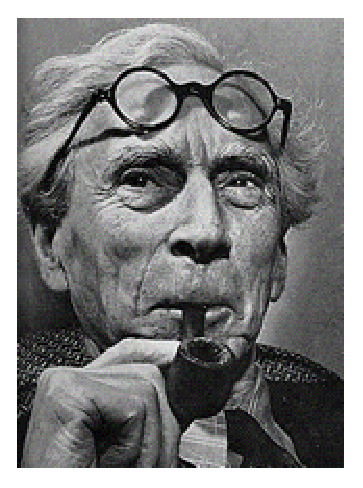
\includegraphics[width=140pt]{russell.eps} \hspace*{30pt} &
	\hspace*{30pt} 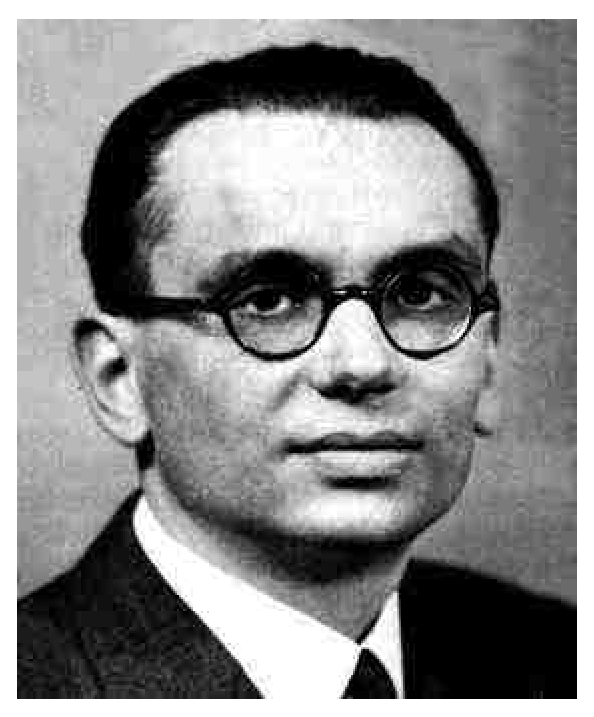
\includegraphics[width=150pt]{godel.eps}
	\end{tabular}
	\end{center}
	\caption[]{Bertrand Russell 1872--1970 (izquierda), Kurt G\"odel 1906--1978 (derecha).}
\end{figure}

Russell fué un filósofo y matemático inglés y es conocido principalmente por sus aportes en lógica matemática y filosofía analítica.
Russell descubrió su paradoja justo cuando el matemático alemán Gottlob Frege (1848--1925) terminaba de escribir el segundo tomo de su libro \emph{The Basic Laws of Arithmetic} que pretendía dictar las pautas de la matemática en ese momento.
La paradoja de Russell puso en jaque el trabajo de Frege, principalmente porque en este se tomaba el axioma de abstracción como base para la construcción de conjuntos y por lo tanto se basaba en un hecho matemático contradictorio, lo que desmoronaba completamente la teoría.
La paradoja de Russell llegó a manos de Frege en el momento en que su libro ya se encontraba en la imprenta para ser publicado.
Frege debió entonces abortar la publicación y agregar un capítulo final a su libro sólo para intentar lidiar con la paradoja de Russell.
\end{nota}

>Dónde está el problema?
Principalmente por el hecho de considerar ``conjuntos muy grandes'' o ``colecciones de demasiados elementos''.
Esto es posible gracias a lo permisivo del axioma de abstracción.
La moraleja es que no cualquier propiedad puede ser tomada para crear un conjunto, en particular la propiedad $\varphi(x)\Leftrightarrow x\notin x$ no es una propiedad válida para crear un conjunto.

\subsubsection*{Axioma de Separación}
El axioma de abstracción es desechado por el hecho de que lleva a una contradicción.
Para reemplazarlo existe el \emph{Axioma de Separación}.
Este nos dice que para crear un conjunto, podemos usar una propiedad cualquiera pero sólo acerca de elementos que existen ya en otro conjunto que ha si creado ``sanamente''.
Con ``sanamente'' nos referimos a conjuntos que no han sido creados a partir del axioma de abstracción.
Con esto, podemos afirmar que, si $\varphi$ es una propiedad y $C$ es un conjunto entonces
\[
A=\{x\;|\;x\in C\text{ y }\varphi(x)\}
\]
también es un conjunto.
El conjunto $A$ se forma entonces \emph{separando} de $C$ los elementos que cumplen $\varphi$.

En el resto de estos apuntes muchas veces definiremos conjuntos usando simplemente una propiedad, en esos casos se supondrá que los elementos los estamos tomando de un conjunto ``universal sano'' que llamaremos $\mathcal{U}$, así cuando nos refiramos al conjunto $A=\{x\;|\;\varphi(x)\}$ realmente nos estaremos refiriendo a
\[A=\{x\;|\;x\in\mathcal{U}\text{ y }\varphi(x)\}.
\]

\begin{nota}
Estos axiomas, junto a otros (Axioma de Pares, de Uniones, del Conjunto Potencia, de Regularidad, de Reemplazo) que no enunciaremos pero veremos desde un punto de vista intuitivo, forman la base de la teoría de conjuntos.

El Axioma de Separación, evita la paradoja o contradicción de Russell que surgía ante el Axioma de Abstracción, la pregunta que uno podría hacerse es mayor,
>son los axiomas libres de otras contradicciones? 
>está la matemática (teoría de conjuntos) libre de contradicciones?
>es posible demostrar que no hay contradicciones en la matemática?
En cuanto a las primeras dos preguntas, hasta hoy no hay contradicciones conocidas, si las hubiera no tendría sentido estudiar esta teoría.
En cuanto a la última pregunta la respuesta es increíblemente NO, no es posible demostrar la consistencia (libertad de contradicción) de la matemática dentro de la matemática, o sea, la matemática no puede demostrar su propia consistencia.
Esta respuesta la dio el matemático Kurt G\"{o}del (1906--1978) en el año 1933.
Kurt G\"odel junto a Bertrand Russell son considerados los lógicos matemáticos mas importantes del siglo XX.

\end{nota}

\subsubsection*{Operaciones}
A partir de conjuntos dados es posible crear nuevos conjuntos aplicando operaciones entre ellos.
Sean $A$ y $B$ conjuntos, entonces las siguientes son operaciones elementales y el resultado de cada una es un conjunto\footnote{Aquí introduciremos una notación que esperamos se mantenga durante el desarrollo de los apuntes. En general para los elementos de conjuntos usaremos letras minúsculas como $x$, $y$ o $z$, para los conjuntos usaremos letras mayúsculas como $A$, $B$, o $C$ y para los conjuntos cuyos elementos son conjuntos usaremos letras cursivas como $\mathcal{R}$, $\mathcal{S}$ o $\mathcal{T}$.}:
\begin{itemize}
  \itemsep 0pt
  \item Unión: $A\cup B=\{x\;|\;x\in A\text{ o } x\in B\}$, los elementos que están en $A$ o en $B$.
  \item Intersección: $A\cap B=\{x\;|\;x\in A\text{ y } x\in B\}$, los elementos que simultáneamente están en $A$ y en $B$.
  \item Diferencia: $A\setminus B=\{x\;|\;x\in A\text{ y } x\notin B\}$, los elementos que están en $A$ pero no en $B$. 
  A veces escribiremos simplemente $A-B$ refiriéndonos a la diferencia de conjuntos.
  %\item Singleton: $\mathcal{S}(A)=\{A\}$, el conjunto que sólo tiene a $A$ como conjunto.
  \item Conjunto Potencia: $\P(A)=\{X\;|\;X\subseteq A\}$, el conjunto de todos los subconjuntos de $A$.
\end{itemize}

Estas operaciones ya debieran ser familiares para el alumno.
De ellas, tal vez el concepto más interesante es el del conjunto potencia, nótese que si $A$ es un conjunto cualquiera, entonces siempre se cumple que $\emptyset\in\P(A)$ y que $A\in\P(A)$ (>por qué?).
Otras propiedades que satisfacen estas operaciones son por ejemplo que para todos los conjuntos $A$ y $B$ se tiene que $A\subseteq A\cup B$ y que $A\cap B\subseteq A$.

\begin{ejemplo}[Construcción de los Naturales.]
Hasta ahora el único conjunto que sabemos con certeza que existe es el conjunto vacío $\emptyset$.
A partir de él podemos generar otros conjuntos usando el siguiente operador:
\[
\sigma(x)=x\cup\{x\}.
\]
Con el podríamos inductivamente hacer la siguiente construcción:
\[
\begin{array}{rcll}
0 & = & \emptyset \\
1 & = & \sigma(\emptyset) = \sigma(0) = \sigma(\emptyset) = \emptyset\cup\{\emptyset\} = \{\emptyset\} = \{0\}\\
2 & = & \sigma(\sigma(\emptyset)) = \sigma(1) = \sigma(\{\emptyset\}) = \{\emptyset\}\cup\{\{\emptyset\}\} = \{\emptyset,\{\emptyset\}\} = \{0,1\} \\
3 & = & \sigma(\sigma(\sigma(\emptyset))) = \sigma(2) = \sigma(\{\emptyset,\{\emptyset\}\}) = \{\emptyset,\{\emptyset\}\}\cup\{\{\emptyset,\{\emptyset\}\}\} = \{\emptyset,\{\emptyset\},\{\emptyset,\{\emptyset\}\}\} = \{0,1,2\}\\
%4 & = & \;\;\;\;\;\;\;\; \cdots \;\;\;\;\;\;\;\; = \{0,1,2,3\}\\
\vdots
\end{array}
\]
El operador $\sigma$ puede considerarse como el operador \emph{sucesor}, así el {\bf conjunto sucesor} de un conjunto $N$ es $\sigma(N)$.
La idea de esta construcción es que al conjunto vacío le llamamos $0$, al conjunto sucesor del conjunto vacío, o sea $\sigma(\emptyset)$, le llamamos $1$, al conjunto sucesor del conjunto sucesor del conjunto vacío, o sea $\sigma(\sigma(\emptyset))$, le llamamos $2$ y así continuamos hasta crear todos los naturales.

Con esto mostramos que la simple existencia del conjunto vacío basta para crear a todos los naturales, partiendo de que al $\emptyset$ se le llama $0$ y usando el operador sucesor $\sigma$.

Dado que tenemos una definición formal inductiva de los números naturales, podemos definir las operaciones sobre ellos como por ejemplo la suma:
\begin{enumerate}
	\itemsep 0pt
	\item $\text{sum}(m,0)=m$
	\item $\text{sum}(m,\sigma(n))=\sigma(\text{sum}(m,n))$
\end{enumerate}
Como ejercicio el alumno podría demostrar que efectivamente $3+4=7$, que la operación suma es conmutativa, que es asociativa, etc.
También se puede definir, de manera similar a la función sum, la función mult para multiplicar dos naturales.
\end{ejemplo}

\subsubsection*{Leyes de la Teoría}
Consideremos un conjunto $\U$ (universal) fijo.
Sea $A\subseteq\U$ un conjunto cualquiera, definimos $A^c$ el \emph{complemento} de $A$ (relativo a $\U$) como
\[
A^c=\U\setminus A=\{x\;|\;x\in\U\text{ y } x\notin A\}.
\]

\begin{teorema}
Sean $A,B$ y $C$ conjuntos cualquiera subconjuntos de $\U$, entonces se cumplen las siguientes leyes:
\begin{multicols}{2}
\begin{enumerate}
  \itemsep 0pt
  \item Asociatividad
  \[
  \begin{array}{l}
  A\cup(B\cup C)=(A\cup B)\cup C, \\
  A\cap(B\cap C)=(A\cap B)\cap C.
  \end{array}
  \]
  \item Conmutatividad
  \[
  \begin{array}{l}
  A\cup B=B\cup A,\\
  A\cap B=B\cap A.
  \end{array}
  \]
  \item Idempotencia
  \[
  \begin{array}{l}
  A\cup A=A, \\ A\cap A=A.
  \end{array}
  \]
  \item Absorción
  \[
  \begin{array}{l}
  A\cup(A\cap B)=A,\\ A\cap(A\cup B)=A.
  \end{array}
  \]
  \item Elemento Neutro
  \[
  \begin{array}{l}
  A\cup\emptyset=A,\\ A\cap\U=A.
  \end{array}
  \]
  \item Distributividad
  \[
  \begin{array}{l}
  A\cup(B\cap C)=(A\cup B)\cap(A\cup C),\\ A\cap(B\cup C)=(A\cap B)\cup(A\cap C).
  \end{array}
  \]
  \item Leyes de De Morgan
  \[
  \begin{array}{l}
  (A\cup B)^c=A^c\cap B^c,\\ (A\cap B)^c=A^c\cup B^c.
  \end{array}
  \]
  
  \item Elemento Inverso
  \[
  \begin{array}{l}
  A\cup A^c=\U, \\ A\cap A^c=\emptyset
  \end{array}
  \]
  
  \item Dominación: 
  \[
  \begin{array}{l}
  A\cup\U=\U,\\ A\cap\emptyset=\emptyset.
  \end{array}
  \]
\end{enumerate}
\end{multicols}
\begin{demostracion}
Ejercicio.
\end{demostracion}
\end{teorema}

\subsubsection{Operaciones Generalizadas}
Sea $\mathcal{S}$ un conjunto de conjuntos, podemos definir:
\[
\bigcup \mathcal{S}=\{x\;|\;\exists X\in\mathcal{S}\text{ tal que }x\in X)\},
\]
y de forma equivalente
\[
\bigcap \mathcal{S}=\{x\;|\;\text{para todo } X\in\mathcal{S}\text{ se cumple que }x\in X)\}.
\]
El primero representa a la unión de todos los conjuntos componentes de $\mathcal{S}$, el segundo a la intersección de estos.
A veces nos referiremos a ellos usando la notación:
\[
\bigcup \mathcal{S}=\bigcup_{A\in\mathcal{S}}A
\]
%\text{\hspace*{30pt} y \hspace*{30pt}} 
\[
\bigcap\mathcal{S}=\bigcap_{A\in\mathcal{S}}A.
\]

Si $\mathcal{S}=\{X_0,X_1,\ldots,X_{n-1}\}$, o sea, una colección indexada de conjuntos, entonces usaremos:
\[
\bigcup \mathcal{S}=X_0\cup X_1\cup\cdots X_{n-1}=\bigcup_{i=0}^{n-1}X_i
\]
%\text{\hspace*{20pt} y \hspace*{20pt}}
\[
\bigcap \mathcal{S}=X_0\cap X_1\cap\cdots X_{n-1}=\bigcap_{i=0}^{n-1}X_i.
\]
En estos casos podremos decir que $x\in\bigcup_{i=0}^{n-1}X_i\Leftrightarrow \exists i$, $0\leq i<n$ tal que $x\in X_i$, y que $x\in\bigcap_{i=0}^{n-1}X_i\Leftrightarrow \text{ para todo } i$, $0\leq i<n$ se tiene que $x\in X_i$.

Si $\mathcal{S}=\{X_0,X_1,\ldots,X_{n-1},X_n,\ldots\}$, o sea, una colección infinita\footnote{En estricto rigor debiéramos decir \emph{infinita enumerable}.
Más adelante en el curso formalizaremos esta noción.} de conjuntos, entonces:
\[
\bigcup \mathcal{S}=X_0\cup X_1\cup\cdots X_{n-1}\cup X_n\cup\cdots=\bigcup_{i=0}^\infty X_i
%\text{\hspace*{10pt} y \hspace*{10pt}} 
\]\[
\bigcap \mathcal{S}=X_0\cap X_1\cap\cdots X_{n-1}\cap X_n\cap\cdots=\bigcap_{i=0}^\infty X_i.
\]
En estos casos podremos decir que $x\in\bigcup_{i=0}^\infty X_i\Leftrightarrow \exists i\in\N$ tal que $x\in X_i$, y que $x\in\bigcap_{i=0}^\infty X_i\Leftrightarrow \text{ para todo } i\in\N$ se tiene que $x\in X_i$.

No es difícil notar que $A\cup B=\bigcup\{A,B\}$ y que $A\cap B=\bigcap\{A,B\}$.

\begin{ejemplo}
Un ejemplo muy simple, si $\mathcal{S}=\{\{1,2,3,4\},\{2,3,4,5\},\{3,4,5,6\}\}$ entonces se cumple que
\[
\bigcup\mathcal{S}=\{1,2,3,4,5,6\}\text{ y }\bigcap\mathcal{S}=\{3,4\}.
\]
\end{ejemplo}

\begin{ejemplo}
Sea $N$ el $N$--ésimo conjunto creado según las reglas del ejemplo de la {\bf construcción de los naturales} de esta sección, o sea, $N$ se forma al aplicar $N$ veces el operador $\sigma$ al conjunto vacío, entonces se cumple que
\[
\bigcap N=\emptyset\text{\hspace*{10pt} y \hspace*{10pt}}\bigcup N=N-1
\]
donde $N-1$ es el \emph{nombre} del conjunto que se forma a partir de aplicar $N-1$ veces el operador $\sigma$ al conjunto vacío.

\begin{demostracion}
$N$ resulta de aplicar $N$ veces $\sigma$ al conjunto vacío, o al 0 si es que usamos los nombres de los números naturales.
Además sabemos que podemos escribir $N=\{0,1,2,\ldots,N-1\}$ suponiendo que seguimos la misma norma de \emph{llamar} $N-1$ al conjunto que se crea por aplicar $N-1$ veces el operador $\sigma$ al conjunto vacío (importante es notar que $N-1$ es sólo un nombre para un conjunto, en ningún caso está representando la resta del conjunto $N$ con el conjunto $1$).
Dado que $0=\emptyset$ y $0\in N$ entonces $\bigcap N=\emptyset$, ahora para calcular $\bigcup N$ podemos hacer lo siguiente:
\[
\bigcup N=\bigcup\{0,1,2,\ldots,N-1\}=0\cup 1\cup 2\cup\cdots\cup N-1,
\]
de donde obtenemos que
\[
\bigcup N=0\cup\{0\}\cup\{0,1\}\cup\{0,1,2\}\cup\cdots\cup\{0,1,\ldots,N-2\},
\]
y dado que $0=\emptyset$ resulta que
\[
\bigcup N=\{0,1,2,\ldots,N-2\}=N-1.
\]
\end{demostracion}
\end{ejemplo}

\newpage
\section{Relaciones}
Las relaciones son un concepto muy usado en computación, principalmente en el ámbito de las Bases de Datos (Bases de Datos Relacionales).
Intuitivamente una relación matemática puede verse como una \emph{correspondencia} de objetos de distintos dominios.
Generalmente en el contexto de Bases de Datos, esta correspondencia está dada por una tabla.
Por ejemplo la siguiente tabla muestra un trozo de la correspondencia entre alumnos y los cursos que ellos están tomando durante este semestre:
\begin{center}
\begin{tabular}{l|l}
{\bf Alumno} & {\bf Curso} \\ \hline
Aliaga & Lenguajes Formales \\
Aliste & Modelos Discretos \\
Aliste & Algoritmos y Estructuras de Datos \\
Arias &  Modelos Discretos \\
Arias &  Algoritmos y Estructuras de Datos \\
Acevedo & Algotimos y Estructuras de Datos \\
Bravo & Lenguajes Formales \\
\vdots & \vdots
\end{tabular}
\end{center}
Esta correspondencia nos dice por ejemplo que el alumno Aliaga está tomando el curso de Lenguajes Formales y que el alumno Aliste está tomando el curso de Modelos Discretos y de Algoritmos y Estructuras de Datos.

En esta sección formalizaremos el concepto de relación matemática y veremos diversas aplicaciones de él.

Lo primero que se debe definir para estudiar relaciones es el concepto de par ordenado:

\begin{definicion}
Se define el \emph{par ordenado} $(a,b)$ de los elementos $a$ y $b$ ambos elementos de un conjunto universal $\U$, de la siguiente manera:
\[
(a,b)=\{\{a\},\{a,b\}\}.
\]
La idea detrás de esta definición es que dos pares ordenados son iguales si y sólo si sus \emph{componentes} son iguales por separado, es decir:
\[
(a,b)=(c,d)\text{ si y sólo si }a=c\wedge b=d.
\]
Como ejercicio se puede demostrar esta propiedad a partir de la definición.
\end{definicion}
Esta definición se puede extender para soportar \emph{tríos ordenados} $(a,b,c)=((a,b),c)$, \emph{cuadruplas ordenadas} $(a,b,c,d)=((a,b,c),d)$ y en general, $n$--tuplas ordenadas $(a_1,a_2,\ldots,a_n)=((a_1,a_2,\ldots,a_{n-1}),a_n)$.
La siguiente definición importante en el contexto de las relaciones matemáticas es la de producto cartesiano.

\begin{definicion}
Sea $A$ y $B$ conjuntos subconjuntos de un conjunto universal $\U$, se define el \emph{producto cartesiano} entre $A$ y $B$, $A\times B$ como
\[
A\times B=\{(a,b)\;|\;a\in A\wedge b\in B\},
\]
o sea, $A\times B$ es el conjunto de todos los pares ordenados tales que su primera componente está en $A$ y su segunda en $B$.
\end{definicion}
Esta definición también se puede extender al producto cartesiano entre varios conjuntos, $A_1\times A_2\times\cdots\times A_n$.
Ahora podemos definir lo que es una relación:

\begin{definicion}
Sean $A$ y $B$ conjuntos, $R$ es una \emph{relación binaria} de $A$ en $B$ si 
\[
R\subseteq A\times B.
\]
Similarmente $R$ se dice una relación binaria \emph{sobre} $A$ si
\[
R\subseteq A\times A.
\]
\end{definicion}

\begin{ejemplo}
Supongamos que $A$ es el conjunto de todos los nombres de alumnos de la carrera de computación y que $B$ es el conjuntos de todos los nombres de cursos de computación, entonces la tabla que relaciona cada alumno con los cursos que está tomando este semestre es una relación binaria de $A$ en $B$.
Llamemos ${\it CargaComp}$ a esa relación, es claro que ${\it CargaComp}\subseteq A\times B$.
De hecho en $A\times B$ aparecen todos los pares posibles de nombres de alumnos y nombres de cursos, sin embargo en ${\it CargaComp}$ aparecen sólo aquellas en las que el alumno pertenece al curso en este semestre.
Por ejemplo, el par 
\[
(\text{Aliste, Lenguajes Formales})\in A\times B,
\]
sin embargo 
\[
(\text{Aliste, Lenguajes Formales})\notin {\it CargaComp}.
\]
\end{ejemplo}

Es posible extender el concepto de relación binaria a relación $n$--aria sobre más de dos conjuntos.
$R$ es una relación $n$--aria si $R\subseteq A_1\times A_2\times\cdots\times A_n$.
De hecho este es mucho más el caso que ocurre en las bases de datos.
Es muy común tener por ejemplo una tabla con información de personas que relacionan el RUT de una persona, con su nombre, teléfono, dirección, edad, etc.

En nuestro estudio estaremos generalmente interesados en relaciones binarias casi siempre sobre un único conjunto.
Para una relación binaria $R$, si el par $(a,b)$ está relacionado por $R$, o sea $(a,b)\in R$, escribiremos también $aRb$, de la misma manera si el par no está relacionado escribiremos $a\nr Rb$.
Esta notación debiera ser familiar para el alumno por ejemplo en relaciones de desigualdad, de hecho para un par que está relacionado por la relación \emph{menor o igual} no escribimos $(a,b)\in\leq$ si no más bien $a\leq b$, y si el par no está relacionado escribimos $a\not\leq b$.

\begin{ejemplo}
\begin{enumerate}
  \itemsep 0pt
  \item Sea $A=\{a,b,c,d,e\}$ entonces el siguiente conjunto es una relación sobre $A$.
  \[
  R=\{(a,b),(b,b),(b,c),(c,b),(c,d),(d,a),(d,b),(d,c),(d,d),(d,e)\}.
  \]
  Decimos por ejemplo que $aRb$, $dRc$, $a\nr Rd$ y $c\nr Re$.
  \item
	La relación \emph{divide a}, denotada por $|$, sobre los naturales sin el $0$, es una relación tal que $a$ está relacionado con $b$ si y sólo si $b$ es un múltiplo de $a$,
	\[
	%|\subseteq(\N-\{0\})\times(\N-\{0\}),\hspace*{3em}
	a|b\text{ si y sólo si }\exists k\in\N\text{ tal que }b=ka.
	\]
	Entonces sabemos que $3|9$ y que $18|72$ pero que $7\hspace*{-0.5em}\not |9$.
	Algo más que podríamos decir es que, por ejemplo, $1$ y $17$ son los únicos naturales relacionado \emph{por la izquierda} con $17$ (>por qué?).
	
	\item
	La relación \emph{equivalencia módulo $n$} con $n\in\N$, que denotaremos por $\equiv_n$, sobre los naturales, es una relación tal que $a$ está relacionado con $b$ si y sólo si $|a-b|$ es múltiplo de $n$.
	\[
	%\equiv_n\subseteq \N\times\N,\hspace*{3em}
	a\equiv_nb\text{ si y sólo si }\exists k\in\N\text{ tal que }|a-b|=kn.
	\]
	Entonces si por ejemplo $n=7$, sabemos que $2\equiv_723$, $8\equiv_71$, $19\not\equiv_74$.
	Algo más que podríamos decir es que por ejemplo, para todo $n\in\N$ se cumple que $0\equiv_nn$.
	
	\item
	Sea $\U$ un conjunto cualquiera y sea $C\subseteq\U$ un subconjunto fijo de $\U$.
	Podemos definir la relación $\mathcal R_C$ sobre $\P(\U)$ (el conjunto potencia de $\U$), tal que $A$ está relacionado con $B$, si y sólo si $A$ y $B$ tienen los mismos elementos en común con $C$.
	\[
	%\mathcal R_C\subseteq\P(\U)\times\P(\U),\hspace*{3em}
	A\mathcal R_CB\text{ si y sólo si }A\cap C=B\cap C.
	\]
	Podríamos decir por ejemplo que $\forall X\in\P(\U)$, si $X\cap C=\emptyset$ entonces $XR_C\emptyset$.
	Además, si $CR_CX$ entonces necesariamente se cumple que $C\subseteq X$.
\end{enumerate}
\end{ejemplo}

\subsection{Propiedades de las Relaciones Binarias}
\label{sec:prop-rel}
\begin{definicion}
Sea $R$ una relación sobre un conjunto $A$.
$R$ se dice:
\begin{itemize}
	\item 
	\emph{Refleja} (o \emph{reflexiva}) si para todo $x\in A$, $x$ está relacionado con $x$ mediante $R$.
	\[
	R\text{ es refleja si y sólo si }\forall x\in A\text{ se cumple que }xRx
	\]
	
	\item
	\emph{Simétrica} si cada vez que el par $(x,y)$ está relacionado por $R$, el par $(y,x)$ también lo está.
	\[
	R\text{ es simétrica si }xRy\Rightarrow yRx
	\]
	
	\item
	\emph{Asimétrica} si cada vez que el par $(x,y)$ está relacionado por $R$, el par $(y,x)$ no está relacionado por $R$.
	\[
	R\text{ es asimétrica si }xRy\Rightarrow y\nr Rx
	\]
	
	\item
	\emph{Antisimétrica} si la única forma de que los pares $(x,y)$ e $(y,x)$ estén relacionados, es cuando $x=y$.
	\[
	R\text{ es antisimétrica si }xRy\wedge yRx\Rightarrow x=y
	\]
	
	\item
	\emph{Transitiva} si cada vez que los pares $(x,y)$ e $(y,z)$ están relacionados, entonces el par $(x,z)$ también está relacionado por $R$.
	\[
	R\text{ es transitiva si }xRy\wedge yRz\Rightarrow xRz
	\]
\end{itemize}
\end{definicion}
\begin{ejemplo}
\begin{enumerate}
  \itemsep 0pt
  \item La relación $|$ es refleja, antisimétrica y transitiva.
  Demostraremos las propiedades de antisimetría y transitividad, la reflexividad se deja como ejercicio.
  
  Para demostrar antisimetría, debemos probar que si ocurre que $a|b$ y $b|a$ entonces necesariamente $a=b$.
  Supongamos que $a|b$, entonces sabemos que existe un $k_1\in\N$ tal que $k_1a=b$, por otro lado, si además $b|a$ entonces sabemos que existe un $k_2\in\N$ tal que $k_2b=a$.
  De estas dos igualdades obtenemos $k_1k_2b=b$ de donde concluimos que
  \[
  k_1k_2=1\hspace*{3em}\text{con }k_1,k_2\in\N.
  \]
  La única forma de que esto sea cierto para dos naturales es que ambos sean $1$, por lo que necesariamente $a=b$.
  Hemos demostrado que $a|b\wedge b|a\Rightarrow a=b$.
  
  Demostraremos ahora transitividad.
  Supongamos que $a|b$ y que $b|c$, por definición sabemos que existen $k_1,k_2\in\N$ tales que $k_1a=b$ y $k_2b=c$.
  Uniendo estas últimas igualdades obtenemos $k_1k_2a=c$, y ya que $k_1k_2\in\N$ concluimos que $a|c$.
  Hemos demostrado que $a|b\wedge b|c\Rightarrow a|c$.
  
  \item 
 	La relación $\equiv_n$ es refleja, simétrica y transitiva.
 	Demostraremos sólo la transitividad, las otras propiedades se dejan como ejercicio.
 	Supongamos que $x\equiv_ny$ y que $y\equiv_nz$, entonces existen $k_1,k_2\in\N$ tales que $|x-y|=k_1n$ y $|y-z|=k_2n$.
 	Dependiendo de los valores de $x,y$ y $z$ se pueden dar cuatro casos:
 	\[
 	\begin{array}{rr}
 	x-y=k_1n & y-z=k_2n \\
 	x-y=-k_1n & y-z=-k_2n
 	\end{array}
 	\]
 	trataremos de analizar los cuatro simultáneamente.
 	Sea $y-z=\pm k_1n$, por lo que $y=\pm k_1n+z$, reemplazando en la otra igualdad obtenemos $x-(\pm k_1n+z)=\pm k_2n$ de donde se concluye que 
 	\[
 	x-z=(\pm k_1+\pm k_2)n. 
 	\]
 	Si tomamos valor absoluto a esta última igualdad obtenemos
 	\[
 	|x-z|=|\pm k_1+\pm k_2|n
 	\]
 	de donde si $k_3=|\pm k_1+\pm k_2|$, $k_3\in\N$ y $|x-z|=k_3n$ y por lo tanto $x\equiv_nz$.
 	
 	\item La relación $R_C$ definida en el ejemplo anterior, es refleja, simétrica y transitiva.
 	Las demostraciones resultan directas de las propiedades del operador $\cap$ y se dejan como ejercicio.
\end{enumerate}
\end{ejemplo}

Se pueden definir distintos tipos de relaciones según las propiedades que estas tengan.
Más adelante estudiaremos dos tipos muy importantes.

\subsection{Representación Matricial}
Si tenemos una relación $R$ sobre un conjunto finito $A$, esta puede representarse mediante una matriz binaria (con sólo ceros y unos).
Esta representación es muy conveniente si queremos que un computador procese información, opere relaciones o decida propiedades acerca de la relación.
Para obtener la representación, etiquetamos tanto las columnas como filas de la matriz con elementos de $A$ en algún orden arbitrario.
Un $1$ en la posición $(i,j)$ de la matriz indica que los elementos correspondientes a la fila $i$ columna $j$ están relacionados, un $0$ en cambio india que no están relacionados.
Generalmente a la matriz que representa a la relación $R$ la llamaremos $M_R$.

\begin{ejemplo}
Sea $A=\{a,b,c,d,e\}$, el siguiente conjunto es una relación sobre $A$.
  \[
  R=\{(a,b),(b,b),(b,c),(c,b),(c,d),(d,a),(d,b),(d,c),(d,d),(d,e)\}.
  \]
  La matriz que representa a $R$ es
  \[
  M_R=
  \left[
  \begin{array}{c c c c c}
  0 & 1 & 0 & 0 & 0 \\
  0 & 1 & 1 & 0 & 0 \\
  0 & 1 & 0 & 1 & 0 \\
  1 & 1 & 1 & 1 & 1 \\
  0 & 0 & 0 & 0 & 0 
  \end{array}\right]
  \]
  en donde las filas y columnas se han etiquetado en orden alfabético.
\end{ejemplo}

>Cómo puedo de forma simple analizando la matriz $M_R$ determinar si $R$ es refleja, simétrica, etc.?
No es difícil notar que $R$ es refleja si y sólo si $M_R$ tiene toda la diagonal con $1$'s y que es simétrica si $M_R=(M_R)^T$.
Para formalizar estas nociones intuitivas introduciremos ciertos conceptos.

\begin{definicion}
Sean $R$ y $S$ dos relaciones sobre el conjunto finito $A$ de $n$ elementos, y $M_R$ y $M_S$ las matrices representantes respectivamente.
Llamaremos $[M_R]_{(i,j)}$ a la componente $(i,j)$ de la matriz $M_R$.
\begin{enumerate}
  \itemsep 0pt
  \item Diremos que $M_R$ es menor o igual a $M_S$ y escribiremos $M_R\leq M_S$ si para todo par $(i,j)$ se cumple que $[M_R]_{(i,j)}\leq[M_S]_{(i,j)}$.
  Note que $M_R\leq M_S$ si y sólo si cada vez que $[M_R]_{(i,j)}=1$ entonces ocurre que $[M_S]_{(i,j)}=1$, $M_S$ tiene $1$'s al menos en todas las posiciones en que $M_R$ tiene $1$'s (y posiblemente en otras posiciones más).
  \item Definimos la \emph{disyunción} o suma lógica $M_R\vee M_S$ como la matriz cuyas componentes cumplen 
  \[
  [M_R\vee M_S]_{(i,j)}=\left\{
  						\begin{array}{lr}
  						1 & \text{ si }[M_R]_{(i,j)}=1\text{ o }[M_S]_{(i,j)}=1 \\
  						0 & \text{ en otro caso.}
  						\end{array}\right.
  \]
  \item Definimos la \emph{conjunción} $M_R\wedge M_S$ como la matriz cuyas componentes cumplen
  \[
  [M_R\wedge M_S]_{(i,j)}=\left\{
  						\begin{array}{lr}
  						1 & \text{ si }[M_R]_{(i,j)}=1\text{ y }[M_S]_{(i,j)}=1 \\
  						0 & \text{ en otro caso.}
  						\end{array}\right.
  \]
  \item Definiremos la multiplicación $M_R\cdot M_S$ como la matriz cuyas componentes se forman al multiplicar ambas matrices de la manera usual del álgebra de matrices,
  \[
  [M_R\cdot M_S]_{(i,j)}=\sum_{l=1}^n[M_R]_{(i,l)}[M_S]_{(l,j)}
  \] 
  pero suponiendo suma booleana, es decir, suponiendo que $1+1=1$.
  De la misma manera podemos definir la potencia $(M_R)^k=M_R\cdot M_R\cdots$ ($k$ veces) $\cdots M_R$.
\end{enumerate}
\end{definicion}

Ahora podemos establecer más formalmente las definiciones intuitivas

\begin{teorema}
\label{teo:propiedades-matrices-relaciones}
Sea $R$ una relación sobre un conjunto $A$ de $n$ elementos y sea $M_R$ la matriz que representa a $R$.
Sea $I_n$ la matriz identidad de $n\times n$.
Se cumple que:
\begin{enumerate}
  \itemsep 0pt
  \item $R$ es refleja si y sólo si $I_n\leq M_R$.
  \item $R$ es simétrica si y sólo si $M_R=(M_R)^T$.
  \item $R$ es antisimétrica si y sólo si $M_R\wedge (M_R)^T\leq I_n$
  \item $R$ es transitiva si y sólo si $M_R\cdot M_R=(M_R)^2\leq M_R$
\end{enumerate}
\begin{demostracion}
A modo de ejemplo demostraremos las propiedades 2 y 4, las otras se dejan como ejercicio:
\begin{enumerate}
  \itemsep 0pt
  \stepcounter{enumi}
  \item Sean $x,y\in A$ y tal que se les han asignado las posiciones $i$ y $j$ dentro de $M_R$ respectivamente.
  
  ($\Leftarrow$) Supongamos que $xRy$ esto implica que $[M_R]_{(i,j)}=1$, dado que que $M_R=(M_R)^T$ tenemos que $[M_R]_{(j,i)}=1$ de donde resulta que $yRx$, por lo que $R$ es simétrica.
  
  ($\Rightarrow$) Supongamos que $[M_R]_{(i,j)}=1$, esto implica que $xRy$, dado que $R$ es simétrica necesariamente $yRx$ por lo que $[M_R]_{(j,i)}=1$. 
  Supongamos ahora que $[M_R]_{(i,j)}=0$, esto implica que $x\nr Ry$ y dado que $R$ es simétrica necesariamente $y\nr Rx$ por lo que $[M_R]_{(j,i)}=0$.
  De los dos argumentos anteriores se concluye que $M_R=(M_R)^T$.
  
  \stepcounter{enumi}
  \item Sean $x,y,z\in A$ y tal que se les han asignado las posiciones $i$, $k$ y $j$ dentro de $M_R$ respectivamente.
  
  ($\Leftarrow$) Sean $x,y,z\in A$ tal que se les han asignado las posiciones $i$, $k$ y $j$ dentro de $M_R$ respectivamente.
  Supongamos que $xRy$ y que $yRz$, por lo que $[M_R]_{(i,k)}=[M_R]_{(k,j)}=1$.
  Analicemos la posición $[(M_R)^2]_{(i,j)}$, esta se forma a partir de la multiplicación $[(M_R)^2]_{(i,j)}=\sum_{l=1}^n[M_R]_{(i,l)}[M_R]_{(l,j)}$, que tiene valor $1$ ya que $[M_R]_{(i,k)}=[M_R]_{(k,j)}=1$.
  Ahora, dado que $(M_R)^2\leq M_R$ necesariamente $[M_R]_{(i,j)}=1$ de donde se concluye que $xRz$.
  Hemos demostrado que cada vez que se cumple $xRy \wedge yRz$ se concluye que $xRz$, por lo tanto $R$ es transitiva.
  
  ($\Rightarrow$) Supongamos que a $x,y\in A$ se les han asignado las posiciones $i$ y $j$ dentro de $M_R$.
  Supongamos ahora que $[(M_R)^2]_{(i,j)}=1$, esto ocurre si y sólo si $\sum_{l=1}^n[M_R]_{(i,l)}[M_R]_{(l,j)}=1$ que ocurre si y sólo si existe un $l$ tal que $[M_R]_{(i,l)}=[M_R]_{(l,j)}=1$, o sea, si y sólo si existe un $v\in A$ tal que $xRv$ y $vRy$.
  Como estamos suponiendo que $R$ es transitiva, necesariamente $xRy$ por lo que $[M_R]_{(i,j)}=1$.
  Demostramos que cada vez que $[(M_R)^2]_{(i,j)}=1$ se cumple que $[M_R]_{(i,j)}=1$ de donde concluimos que $(M_R)^2\leq M_R$.
\end{enumerate}
\end{demostracion}
\end{teorema}

Existe una intima relación entre los operadores matriciales definidos y los operadores de relaciones sobre conjuntos finitos.
Antes de enunciar el siguiente teorema, necesitamos un par de definiciones:

\begin{definicion}
%\begin{enumerate}
%\item 
Sea $R$ una relación binaria de $A$ en $B$.
La \emph{inversa} de $R$, denotada por $R^{-1}$, es la relaón de $B$ en $A$ definida por
  $$
  R^{-1}=\{(x,y)\in B\times A\;|\; yRx\}.
  $$
%  \item 

Sea $R$ una relación binaria de $A$ en $B$ y $S$ una 
  relación binaria de $B$ en $C$.
  La \emph{composición} entre $R$ y $S$, denotada por $R\circ S$,
  es la relación de $A$ en $C$ definida por
  $$
  R\circ S=\{(x,z)\in A\times C\;|\;\text{ existe un }y\in B\text{ tal que }xRy\text{ e }ySz\}.
  $$
%  \end{enumerate}
\end{definicion}

El siguiente teorema relaciona propiedades de las matrices que representan relaciones
y propiedades y operaciones sobre las relaciones mismas.

\begin{teorema}
Sean $R$ y $S$ dos relaciones sobre un conjunto $A$ con $n$ elementos, y $M_R$ y $M_S$ respectivamente las matrices que las representan, entonces se cumple que: \label{teo:operadores-matriz-relacion}
\begin{enumerate}
  \itemsep 0pt
  \item $R\subseteq S$ si y sólo si $M_R\leq M_S$.
  \item La matriz que representa a la relación $R\cup S$ es $M_R\vee M_S$.
  \item La matriz que representa a la relación $R\cap S$ es $M_R\wedge M_S$.
  \item La matriz que representa a $R^{-1}$ es $(M_R)^T$.
  \item La matriz que representa a $R\circ S$ es $M_R\cdot M_S$.
\end{enumerate}
\begin{demostracion} Ejercicio.
\end{demostracion}
\end{teorema}

Se debe tener cuidado con la aplicabilidad de este teorema ya que sólo tiene sentido representar una relación usando matrices cuando esta está definida sobre un conjunto finito.
>Podemos establecer propiedades como en el teorema~\ref{teo:propiedades-matrices-relaciones} para determinar cuándo una relación cualquiera (no necesariamente definida sobre un conjunto finito) cumple con las propiedades de reflexividad, simetría, etc.? 
La respuesta es sí, de hecho el siguiente teorema establece estas propiedades.

\begin{teorema}
\label{teo:propiedades-relaciones}
Sea $R$ una relación cualquiera sobre un conjunto $A$ no necesariamente finito, y sea $D$ la \emph{relación diagonal} definida por $D=\{(x,x)\;|\; x\in A\}$, entonces se cumple que:
\begin{enumerate}
  \itemsep 0pt
  \item $R$ es refleja si y sólo si $D\subseteq R$.
  \item $R$ es simétrica si y sólo si $R=R^{-1}$.
  \item $R$ es antisimétrica si y sólo si $R\cap R^{-1}\subseteq D$.
  \item $R$ es transitiva si y sólo si $R\circ R\subseteq R$.
\end{enumerate}
\begin{demostracion}
Alguien podría estar tentado a argumentar que el teorema es una conclusión directa de los dos teoremas anteriores, esta sería una argumentación correcta sólo en el caso de que la relación estuviese definida sobre un conjunto finito.
Sin embargo este no es el caso, $A$ no necesariamente es finito, por lo que debe entregarse otro argumento.
A modo de ejemplo demostraremos la propiedad 3, las demás se dejan como ejercicio.
\begin{enumerate}
  \itemsep 0pt
  \stepcounter{enumi}
  \stepcounter{enumi}
  \item ($\Leftarrow$) Supongamos que $xRy\wedge yRx$, esto implica que $xRy\wedge xR^{-1}y$ por la definición de $R^{-1}$, y que por lo tanto $(x,y)\in R\cap R^{-1}$.
  Ahora dado que $R\cap R^{-1}\subseteq D$, necesariamente $(x,y)\in D$ de donde se deduce que $x=y$ (es la única forma de que $(x,y)\in D$).
  Hemos demostrado que si $xRy\wedge yRx$ entonces $x=y$ y por lo tanto $R$ es antisimétrica.
  
  ($\Rightarrow$) Sea $(x,y)\in R\cap R^{-1}$ esto implica que $xRy\wedge xR^{-1}y$ y que por lo tanto $xRy\wedge yRx$ por la definición de $R^{-1}$.
  Ahora, dado que $R$ es antisimétrica, si $xRy\wedge yRx$ entonces necesariamente $x=y$ y por lo tanto $(x,y)\in D$.
  Hemos demostrado que si $(x,y)\in R\cap R^{-1}$ entonces $(x,y)\in D$, luego se cumple que $R\cap R^{-1}\subseteq D$.
\end{enumerate}
\end{demostracion}

Nótese que, a pesar de que este teorema no puede establecerse como conclusión a partir de los dos teoremas anteriores (teoremas~\ref{teo:propiedades-matrices-relaciones} y~\ref{teo:operadores-matriz-relacion}), usando este teorema y el teorema~\ref{teo:operadores-matriz-relacion} se concluye inmediatamente el teorema~\ref{teo:propiedades-matrices-relaciones}.
Por ejemplo, dado que para cualquier relación $R$, esta es simétrica si y sólo si $R=R^{-1}$, entonces si $R$ es una relación definida sobre un conjunto finito, dado que $M_{R^{-1}}=(M_R)^T$, $R$ será simétrica si y sólo si $M_R=(M_R)^T$ que es la propiedad 2 del teorema~\ref{teo:propiedades-matrices-relaciones}.
Como ejercicio intente dar una demostración para las demás propiedades del teorema~\ref{teo:propiedades-matrices-relaciones} usando esta idea. 
%\footnote{En el teorema~\ref{teo:propiedades-matrices-relaciones} se usa la matriz $I_n$ para establecer algunas propiedades, note que si $D$ es la relación diagonal sobre un conjunto de $n$ elementos, entonces $M_D=I_n$.}.
\end{teorema}

\subsection{Clausuras}
Muchas veces en computación nos encontramos con relaciones que no cumplen cierta propiedad pero que nos gustaría que la cumplieran para poder obtener información adicional.
En el siguiente ejemplo se motiva este tema.

\begin{ejemplo}
Supongamos que se tiene la siguiente tabla de vuelos directos entre el conjunto $\{$Stgo, BsAs, Miami, Lond, Frnk, Paris, Mosc$\}$ de ciudades del mundo:
\begin{center}
\begin{tabular}{l|l} 
Origen & Destino \\ \hline
Stgo & BsAs \\
Stgo & Miami \\
Stgo & Lond \\
BsAs & Stgo \\
Miami & Stgo \\
Miami & Lond \\
Lond & Stgo \\
Lond & Paris \\
Frnk & Paris \\
Frnk & Mosc \\
Paris & Mosc \\
Mosc & Frnk 
\end{tabular}
\end{center}
Por ejemplo la tabla nos dice que existe un vuelo directo desde Stgo a BsAs y que también existe un vuelo directo desde BsAs a Stgo.
Esto no siempre ocurre, por ejemplo, existe un vuelo directo entre Miami y Lond pero no existe uno entre Lond y Miami.
Es claro que si existe un vuelo directo desde Lond a Stgo y uno desde Stgo a BsAs, entonces es posible llegar desde Lond a BsAs haciendo escala en Stgo.
La pregunta entonces es, dada la relación de vuelos directos >cómo se puede obtener una relación que me indique todos los pares de ciudades tales que existe un vuelo no necesariamente directo, posiblemente con escalas, desde una a la otra?
En lo que sigue de la sección definiremos este problema.
%Si quisiéramos representar esta relación usando una matriz resultaría:
%\[
%M=\left[\begin{array}{ccccccc}
%0 & 1 & 1 & 1 & 0 & 0 & 0 \\
%1 & 0 & 0 & 0 & 0 & 0 & 0 \\
%1 & 0 & 0 & 1 & 0 & 0 & 0 \\
%1 & 0 & 0 & 0 & 0 & 1 & 0 \\
%0 & 0 & 0 & 0 & 0 & 1 & 1 \\
%0 & 0 & 0 & 0 & 0 & 0 & 1 \\
%0 & 0 & 0 & 0 & 1 & 0 & 0 
%\end{array}
%\right]
%\]
\end{ejemplo}
\begin{definicion}
Sea $\varphi$ una propiedad de relaciones sobre un conjunto $A$ (no necesariamente finito), y sea $R$ una relación cualquiera sobre $A$.
Se define la \emph{clausura} $\varphi$ de $R$ como la menor relación que contiene a $R$ y que cumple la propiedad $\varphi$.
Hablaremos de la \emph{clausura refleja} de $R$, \emph{clausura simétrica} de $R$ y \emph{clausura transitiva} de $R$, y la llamaremos $CR(R)$, $CS(R)$ y $CT(R)$ respectivamente.

En la definición aparece el concepto de ``menor relación'', en este contexto menor es con respecto a la relación $\subseteq$, se refiere a que por ejemplo, si $CT(R)$ es la clausura transitiva de $R$, para cualquier otra relación $T$ transitiva que contenga a $R$ se debe cumplir que $CT(R)\subseteq T$.
\end{definicion}

\begin{ejemplo}
En el ejemplo de vuelos directos anterior,
si existe un vuelo directo entre el par de ciudades $(C_1,C_2)$ y otro vuelo directo entre el par $(C_2,C_3)$ en la relación de vuelos posiblemente con escalas nos gustaría tener al par de ciudades $(C_1,C_3)$.
Ahora si por ejemplo también existe un vuelo directo entre el par $(C_3,C_4)$, nos gustaría tener a los pares de ciudades $(C_1,C_4)$ y $(C_2,C_4)$ en la relación de vuelos posiblemente con escalas.
Lo que necesitamos entonces es una relación que contenga a la de vuelos directos pero que además sea transitiva.
Además necesitamos una propiedad muy importante, que la nueva relación no contenga pares de ciudades ``de más'', de hecho no debiera contener el par $($Stgo, Mosc$)$.
La relación de vuelos posiblemente con escalas resulta ser una relación que contiene a la de vuelos directos, que es transitiva y que es la más chica posible, es decir, resulta ser la clausura transitiva de la relación de vuelos directos.

Dado que sabemos que lo que queremos es la clausura transitiva de la relación 
el siguiente paso es preguntarnos cómo podemos obtenerla.
Una posibilidad para enfrentar inicialmente el problema es mirar la matriz que representa a la relación.
En nuestro ejemplo, la matriz resulta ser
\[
M_{V}=\left[\begin{array}{ccccccc}
0 & 1 & 1 & 1 & 0 & 0 & 0 \\
1 & 0 & 0 & 0 & 0 & 0 & 0 \\
1 & 0 & 0 & 1 & 0 & 0 & 0 \\
1 & 0 & 0 & 0 & 0 & 1 & 0 \\
0 & 0 & 0 & 0 & 0 & 1 & 1 \\
0 & 0 & 0 & 0 & 0 & 0 & 1 \\
0 & 0 & 0 & 0 & 1 & 0 & 0 
\end{array}
\right]
\]
en donde las ciudades se han ordenado según su aparición en el conjunto del ejemplo.
Si ahora miramos la matriz al cuadrado obtenemos:
\[
M_V\cdot M_V=\left[\begin{array}{ccccccc}
1 & 0 & 0 & 1 & 0 & 1 & 0 \\
0 & 1 & 1 & 1 & 0 & 0 & 0 \\
1 & 1 & 1 & 1 & 0 & 1 & 0 \\
0 & 1 & 1 & 1 & 0 & 0 & 1 \\
0 & 0 & 0 & 0 & 1 & 0 & 1 \\
0 & 0 & 0 & 0 & 1 & 0 & 0 \\
0 & 0 & 0 & 0 & 0 & 1 & 1 
\end{array}
\right]
\]
$M_V\cdot M_V$ tiene un $1$ en la posición correspondiente al par (BsAs, Miami) el que aparece debido a que en $M_V$ había un $1$ en la posición correspondiente al par (BsAs, Stgo) y un $1$ en la posición correspondiente al par (Stgo, Miami).
Si miramos con más detención, nos daremos cuenta de que cada una de las posiciones que tienen $1$ en $M_V\cdot M_V$ corresponden a pares de ciudades $(C_1,C_2)$ tales que existe un vuelo con una escala intermedia entre $C_1$ y $C_2$.
De la misma forma de podría argumentar que $(M_V\cdot M_V)\cdot M_V$ contiene a todos los pares de ciudades tales que existe un vuelo con dos escalas intermedias entre ellas.
Entonces la matriz
$$M_V\vee(M_V)^2\vee(M_V)^3$$
corresponderá a una relación que tiene todos los pares de ciudades para los cuales existe un vuelo directo, o un vuelo con una escala intermedia, o un vuelo con dos escalas intermedias.
>Cuanto es el máximo número de escalas intermedias que se pueden tener en un vuelo entre un par de ciudades? 
La respuesta es simple, el vuelo más largo que se puede realizar es partir desde una ciudad, pasar por todas las otras ciudades y finalmente volver a la ciudad inicial, por lo que en nuestro caso la matriz
$$M_V\vee(M_V)^2\vee(M_V)^3\vee(M_V)^4\vee(M_V)^5\vee(M_V)^6\vee(M_V)^7$$
representaría a una relación que tiene todos los pares de ciudades $(C_1,C_2)$ para los cuales existe un vuelo posiblemente con escalas intermedias entre $C_1$ y $C_2$, o sea, representaría a la clausura transitiva de la relación de vuelos directos.

El siguiente teorema formaliza esta noción y la de otras clausuras.
\end{ejemplo}

%Dado que sabemos lo que queremos el siguiente paso es pensar en cómo lo obtenemos.
%El siguiente teorema nos entrega una forma de obtener clausuras de relaciones que se encuentran representadas usando matrices.
\begin{teorema}
\label{teo:clausuras-matrices-relaciones}
Sea $R$ una relación sobre un conjunto $A$ de $n$ elementos y sea $M_R$ la matriz que representa a $R$.
Entonces se cumple que:
\begin{enumerate}
  \itemsep 0pt
  \item La matriz que representa a la clausura refleja de $R$ es $$M_{CR(R)}=M_R\vee I_n.$$
  \item La matriz que representa a la clausura simétrica de $R$ es $$M_{CS(R)}=M_R\vee (M_R)^T.$$
  \item La matriz que representa a la clausura transitiva de $R$ es $$M_{CT(R)}=\bigvee_{i=1}^n(M_R)^i.$$ 
\end{enumerate}
\begin{demostracion}
La demostración es una conclusión directa del siguiente teorema que estudiaremos (teorema~\ref{teo:clausuras-relaciones}).
\end{demostracion}
\end{teorema}

Similarmente al teorema~\ref{teo:propiedades-relaciones} que nos daba una equivalencia entre las propiedades de las matrices que representan a una relación y las relaciones definidas no necesariamente sobre conjuntos finitos, podemos establecer un teorema que liga al anterior con clausuras de relaciones en general.

\begin{teorema}
\label{teo:clausuras-relaciones}
Sea $R$ una relación cualquiera sobre un conjunto $A$ no necesariamente finito, y sea $D$ la relación diagonal sobre $A$, entonces se cumple que:
\begin{enumerate}
  \itemsep 0pt
  \item La clausura refleja de $R$, $CR(R)$ se obtiene haciendo $$CR(R)=R\cup D.$$
  \item La clausura simétrica de $R$, $CR(R)$ se obtiene haciendo $$CS(R)=R\cup R^{-1}.$$
  \item La clausura transitiva de $R$, $CT(R)$ se obtiene haciendo $$CT(R)=\bigcup_{i=1}^{\infty}R^{i},$$
  donde $R^i$ representa a la composición $i$ veces $R$, es decir, inductivamente,
  $R^1=R$ y $R^{n+1}=R^{n}\circ R$.
\end{enumerate}
\begin{demostracion}
A modo de ejemplo demostraremos la propiedad 3, las demás se dejan como ejercicio.
\begin{enumerate}
  \itemsep 0pt
  \stepcounter{enumi}
  \stepcounter{enumi}
  \item Para demostrar que $\bigcup_{i=1}^{\infty}R^{i}$ es efectivamente igual a $CT(R)$ se deben demostrar tres cosas: (1) que $\bigcup_{i=1}^{\infty}R^{i}$ contiene a $R$, (2) que $\bigcup_{i=1}^{\infty}R^{i}$ es efectivamente transitiva y (3) que $\bigcup_{i=1}^{\infty}R^{i}$ es subconjunto de cualquier otra relación que contenga a $R$ y sea transitiva. % es subconjunto de .
  Demostraremos cada una por separado:
  \begin{itemize}
  	\itemsep 0pt
    \item[(1)] $\bigcup_{i=1}^{\infty}R^{i}=R\cup R^2\cup R^3\cup\cdots$ por lo que claramente $R\subseteq\bigcup_{i=1}^{\infty}R^{i}$.
    \item[(2)] Supongamos que el par $(x,y)$ e $(y,z)$ pertenecen a $\bigcup_{i=1}^{\infty}R^{i}$, demostraremos que entonces el par $(x,z)$ también pertenece a $\bigcup_{i=1}^{\infty}R^{i}$.
    Si $(x,y)\in\bigcup_{i=1}^{\infty}R^{i}$ entonces necesariamente $(x,y)\in R^j$ para algún $j$, de la misma manera sabemos que $(y,z)\in R^k$ para algún $k$.
    Por la definición de composición, sabemos entonces que el par $(x,z)\in R^j\circ R^k=R^{j+k}$ por lo que $(x,z)$ también pertenece a $\bigcup_{i=1}^{\infty}R^{i}$.
    \item[(3)] Sea $S$ una relación transitiva cualquiera tal que $R\subseteq S$, debemos demostrar que $\bigcup_{i=1}^{\infty}R^{i}\subseteq S$.
%, o sea, que si $(x,y)\in\bigcup_{i=1}^{\infty}R^{i}$ entonces también ocurre que $(x,y)\in S$.
    Demostraremos algo equivalente, demostraremos que para todo $i\geq 1$ se cumple que $R^i\subseteq S$ y por lo tanto $\bigcup_{i=1}^{\infty}R^{i}\subseteq S$.
    Lo haremos usando un argumento inductivo en $i$.
    La base se cumple por la definición de $S$, $R^1=R\subseteq S$.
    Ahora supongamos que $R^i\subseteq S$ y sea $(x,z)\in R^{i+1}$, demostraremos que entonces $(x,z)\in S$ y por lo tanto $R^{i+1}\subseteq S$.
    Si $(x,z)\in R^{i+1}$ entonces $(x,z)\in R^i\circ R$, lo que ocurre sólo si existe un $y$ tal que $(x,y)\in R^i\subseteq S$ e $(y,z)\in R\subseteq S$.
    Ahora dado que $S$ es transitiva y tenemos que $(x,y)\in S\wedge(y,z)\in S$ entonces necesariamente $(x,z)\in S$, por lo que $R^{i+1}\subseteq S$.
  \end{itemize}
\end{enumerate}
\end{demostracion}

Este teorema puede usarse para una demostración directa del teorema~\ref{teo:clausuras-matrices-relaciones}.
Por ejemplo, dado que para cualquier relación $R$ se cumple que $CS(R)=R\cup R^{-1}$ entonces si $R$ es una relación definida sobre un conjunto finito, se tiene que $M_{CS(R)}=M_R\vee M_{R^{-1}}=M_R\vee (M_R)^T$.
\end{teorema}

\subsection{Relaciones de Orden}

\begin{definicion}
Diremos que una relación binaria $R$ sobre un conjunto $A$ es una {\bf relación de orden parcial} si cumple con ser, refleja, antisimétrica y transitiva.
Generalmente cuando $R$ sea una relación de orden parcial la denotaremos por el símbolo $\preceq$.
Si $(x,y)\in\preceq$ o equivalentemente $x\preceq y$, diremos que ``$x$ es menor (o menor--igual) que $y$''.

Diremos además que, si $\preceq$ es una relación de orden parcial sobre $A$, entonces el par $(A,\preceq)$ es un orden parcial.
\end{definicion}

\begin{ejemplo}
\begin{enumerate}
  \itemsep 0pt
	\item Los pares $(\N,\leq)$, $(\Z,\leq)$, $(\R,\leq)$ son todas órdenes parciales.
  \item El par $(\N-\{0\},|)$ es un orden parcial.
  \item Sea $\U$ un conjunto fijo cualquiera, entonces $(\P(\U),\subseteq)$ es un orden parcial.
\end{enumerate}
La demostración de cada una de estas propiedades se deja como ejercicio.
\end{ejemplo}

%\begin{definicion}
%Para cada orden parcial $(A,\preceq)$ existe un orden parcial asociado, $(A,\preceq^{-1})$ el {\bf orden inverso} de $\preceq$.
%Al orden inverso de $\preceq$ lo llamaremos $\succeq$.
%\end{definicion}

>Por qué orden {\bf parcial}?
Parcial, en contraposición a total.
Estamos acostumbrados en los órdenes sobre $\N$, $\Z$ o $\R$, que si no se cumple que $x\leq y$ entonces necesariamente $y\leq x$.
Esto no ocurre en un orden parcial cualquiera, de hecho en el orden $(\N-\{0\},|)$ no ocurre ni que $6|9$ ni que $9|6$.
Tampoco en $(\P(\U),\subseteq)$, de hecho es totalmente posible encontrar un par de conjunto $A$ y $B$ tales que $A\not\subseteq B$ y $B\not\subseteq A$.
Esto motiva la siguiente definición.

\begin{definicion}
Diremos que $(A,\preceq)$ es un {\bf orden total (o lineal)} si es un orden parcial y para cada par de elementos $x,y\in A$ ocurre que $x\preceq y$ o que $y\preceq x$.
\end{definicion}

Cuando hablamos de órdenes parciales (o totales) sobre un conjunto estamos implícitamente estableciendo una estructura sobre el conjunto.
Nos gustaría poder hablar de elementos menores que, mayores que, máximos, mínimos, etc.
Las siguientes definiciones nos hablan de esto:

\begin{definicion}
Sea $(A,\preceq)$ un orden parcial, y sea $S\subseteq A$ un subconjunto no vacio cualquiera de $A$.
Sea $x$ un elemento cualquiera de $A$.
Diremos que:
\begin{enumerate}
	\itemsep 0pt
  \item $x$ es una \emph{cota inferior} de $S$ si para todo $y\in S$ se cumple que $x\preceq y$.
  %de manera similar $x$ será una \emph{cota superior} si para todo $y\in S$ se cumple que $y\preceq x$.
  \item $x$ es un \emph{elemento minimal} de $S$, si $x\in S$ y para todo $y$ en $S$ se cumple que $y\preceq x\Rightarrow y=x$, o sea, $x$ es minimal, si pertenece a $S$ y ningún elemento de $S$ es menor que $x$.
  %De manera similar, $x$ será un \emph{elemento maximal} si $x\in S$ para todo $y$ en $S$ se cumple que $x\preceq y\Rightarrow y=x$.
  \item $x$ es un \emph{mínimo} en $S$, si $x\in S$ y $x$ es cota inferior de $S$.
\end{enumerate}
De manera similar se pueden definir los conceptos de cota superior, elemento maximal, y máximo, por ejemplo, diremos que $x$ es una \emph{cota superior} de $S$ si para todo $y\in S$ se cumple que $y\preceq x$.
\end{definicion}

\begin{ejemplo}
\begin{enumerate}
	\item
	Sea el orden parcial $(\N-\{0\},|)$ y sea $S=\{2,3,5,10,15,20\}\subseteq \N$.
	Podemos decir por ejemplo que $1$ es una cota inferior para $S$, pero que $2$ no es una cota inferior (ya que $2$ no divide a $5$ ni a $15$).
	Podemos decir que $60$ es una cota superior para $S$, ya que $2|60$, $3|60, \ldots, 20|60$, y también $120$ es cota superior.
	$S$ tiene ademas, tres elementos minimales, $2$, $3$ y $5$, y tres elementos maximales $10$, $15$ y $20$.
	Finalmente podemos decir que $S$ no tiene ni mínimo ni máximo.
	>Podemos encontrar un $S\subseteq \N$ tal que todos sus elementos sean maximales y minimales a la vez?
	
	\item 
	Sea el orden parcial $(\P(\{1,2,3,4\}),\subseteq)$ y sea $\mathcal S=\{\{1\},\{1,2\},\{1,3\},\{1,2,3,4\}\}$.
	Podemos decir que $\{1\}$ es una cota inferior, un elemento minimal y un mínimo de $\mathcal S$, y que $\{1,2,3,4\}$ es una cota superior, un elemento maximal y un máximo de $\mathcal S$.
	Otra cota inferior para $\mathcal S$ es $\emptyset$.
	>Podemos encontrar un $\mathcal S\subseteq\P(\{1,2,3,4\})$ tal que todos sus elementos sean maximales y minimales a la vez?
	\end{enumerate}
\end{ejemplo}

\begin{teorema}
Sea $(A,\preceq)$ un orden parcial, y sea $S\subseteq A$ un subconjunto no vacio de $A$.
Si $S$ tiene un elemento mínimo, este es único.

\begin{demostracion}
Supongamos que existen dos elementos mínimos para $S$, digamos $s_1$ y $s_2$.
Dado que son mínimo, tanto $s_1,s_2\in S$ y además se cumple que $s_1\preceq s_2$ y que $s_2\preceq s_1$.
Dado que $\preceq$ es una relación de orden se concluye que $s_1=s_2$ (por antisimetría) y por lo tanto el mínimo es único.
\end{demostracion}

De la misma manera se puede establecer que el máximo de un conjunto es único.
Este teorema nos permite además hablar de él mínimo o él máximo de un conjunto $S$, que anotaremos como $\min(S)$ y $\max(S)$.
\end{teorema}

Note que el teorema dice ``Si $S$ tiene un elemento mínimo...'' esto porque ya vimos en los ejemplos que pueden existir conjuntos sin elementos mínimos.
La siguiente definición extiende el concepto de elemento mínimo.

\begin{definicion}
Sea $(A,\preceq)$ un orden parcial, y sea $S\subseteq A$ un subconjunto cualquiera de $A$.
Sea $x$ un elemento cualquiera de $A$.
Diremos que $s$ es un \emph{ínfimo} de $S$ si $s$ es una cota inferior  de $S$ y para cualquier otra cota inferior $s'$ de $S$ se cumple que $s'\preceq s$.
En palabras, podríamos decir que el ínfimo de $S$ es la mayor de las cotas inferiores de $S$.

De manera similar diremos que $s$ es el \emph{supremo} de $S$ si $s$ es cota superior de $S$ y para cualquier otra cota superior $s'$ de $S$ se cumple que $s\preceq s'$, es decir, el supremo es la menor de las cotas superiores.
\end{definicion}

Un teorema muy similar al de máximos y mínimos se puede establecer para supremos e ínfimos.

\begin{teorema}
Sea $(A,\preceq)$ un orden parcial, y sea $S\subseteq A$ un subconjunto cualquiera de $A$.
Si $S$ tiene supremo, este es único.

\begin{demostracion}
Ejercicio.
\end{demostracion}

De la misma manera se puede establecer que el ínfimo es único.
Este teorema, al igual que para el máximo y el mínimo, nos permite hablar de él supremo o él ínfimo de un conjunto $S$, que anotaremos como $\sup(S)$ y $\inf(S)$.
\end{teorema}

Es totalmente válido que un conjunto cualquiera no tenga mínimo pero si tenga ínfimo, de hecho el alumno debe estar familiarizado con esta noción cuando estudia intervalos abiertos en el orden $(\R,\leq)$.
Por ejemplo el intervalo real abierto $(0,1]$ no tiene un elemento mínimo, sin embargo tiene ínfimo, a saber el $0$.
Siguiendo con $(\R,\leq)$, el intervalo $[1,+\infty)$ no tiene ni máximo ni supremo.

En el orden parcial $(\R,\leq)$ de los reales ocurre además una propiedad bastante importante, todo subconjunto real que es acotado superiormente tiene un supremo.
Esta propiedad también la tienen por ejemplo \mbox{$(\N,\leq)$} y $(\Z,\leq)$.
La pregunta que puede surgir es >existe algún orden parcial que no cumpla esta propiedad?
La respuesta es sí, por ejemplo el orden $(\Q,\leq)$ no cumple esta propiedad.
Para verlo basta mostrar un subconjunto de $\Q$ acotado superiormente que carezca de supremo en $\Q$.
El siguiente conjunto cumple con esta propiedad
\[
S=\{q\in\Q\;|\;q^2\leq 2\}.
\]
Lo primero es notar que $S\subseteq\Q$ y que $S$ es acotado superiormente, de hecho $2\in\Q$ es una cota superior para $S$, pero $S$ no tiene supremo en $\Q$.
Alguien podría estar tentado a refutar esto diciendo que $\sqrt{2}$ es un supremo para $S$, esto no puede ser cierto debido a que $\sqrt{2}\notin\Q$ por lo que no puede ser supremos de ningún subconjunto de $\Q$.
La demostración de que $S$ no tiene supremo se puede hacer por contradicción y se deja como ejercicio (Ayuda: suponga que $s$ es el supremo de $S$ y separe la demostración en dos casos, $s\in S$ y $s\notin S$).

La anterior discusión motiva la siguiente definición.

\begin{definicion}
Sea $(A,\preceq)$ un orden parcial, este se dice {\bf superiormente completo} si para cada subconjunto no vacío $S$ de $A$ se cumple que, si $S$ tiene una cota superior entonces $S$ tiene supremo.

De manera similar un orden es {\bf inferiormente completo} si cada subconjunto no vacío que tiene una cota inferior tiene también ínfimo.
\end{definicion}

Ya vimos que $(\Q,\leq)$ no es superiormente completo
>Es $(\Q,\leq)$ inferiormente completo?
No es difícil notar que el conjunto $S=\{q\in\Q\;|\;2\leq q^2\}$ nos responde la pregunta.
El resultado general está dado por el siguiente teorema.

\begin{teorema}
Sea $(A,\preceq)$ un orden parcial cualquiera, entonces $(A,\preceq)$ es superiormente completo si y sólo si es inferiormente completo.

\begin{demostracion}
Ejercicio. 
%(Ayuda: Suponga que $(A,\preceq)$ es un orden superiormente completo, ahora para demostrar que cada conjunto $S$ acotado inferiormente tiene ínfimo, tome el conjunto $S'=\{x\in A\;|\;\forall y\in S$ $x\preceq y\}$.
%Este conjunto $S'$ está acotado superiormente por lo tanto tiene supremo y apartir del supremo de $S'$ demuestre que $S$ tiene ínfimo.)
\end{demostracion}
\end{teorema}

Las relaciones de orden establecen una estructura sobre los conjuntos en los cuales se definen.
En computación nos interesan principalmente los órdenes sobre conjuntos finitos.
Ya vimos que una relación cualquiera siempre se puede representar usando una matriz binaria, esta también se podría usar para representar un orden parcial.
Veremos una representación alternativa llamada Diagramas de Hasse.
Comenzaremos con un ejemplo.

\begin{ejemplo}
En muchas situaciones se necesita ordenar tareas, debido a que por ejemplo una tarea no puede realizarse si no hasta que otra termine.
Por ejemplo, para vestirse en la mañana una persona debe siempre ponerse la camisa antes que la corbata y definitivamente debe ponerse los calcetines antes de comenzar a abrocharse los cordones de los zapatos.
Sea $T$ entonces un conjunto finito de tareas, definiremos la relación $\mapsto$ sobre $T$ de la siguiente manera:
Sean $t_1$ y $t_2$ tareas en $T$ entonces
\[
t_1\mapsto t_2\Leftrightarrow t_1=t_2\text{, o es necesario terminar la tarea }t_1\text{ antes de comenzar la tarea }t_2.
\]
No es difícil notar que con esta definición $(T,\mapsto)$ se convierte en un orden parcial.
Supongamos que el conjunto de tareas es igual a 
\[
T=\{\text{Calc, Zap, Cord, Calz, Pant, Cint, Camis, Corb, Chal}
\}
\] 
que son todas la tareas que se deben completar para vestirse.
Entonces la relación $\mapsto$ queda definida por:
\[
\begin{array}{rcll}
\mapsto& = \{& \text{(Calc,Calc), (Calc,Zap), (Calc,Cord), (Zap,Zap), (Zap,Cord),(Cord, Cord), (Calz,Calz),} \\ 
& & \text{(Calz,Pant), (Calz,Cint), (Pant,Pant), (Pant,Zap), (Pant,Cint), (Camis, Camis),} \\
& & \text{(Camis,Corb), (Camis,Chal), (Camis,Cint), (Corb,Corb), (Corb,Chal), (Chal,Chal)} & \}
\end{array}
\]
Si quisiéramos buscar una forma consistente de completar todas estas tareas, existen pares que no me entregan información útil, por ejemplo, si sabemos que hay que ponerse los calcetines antes que los zapatos y que hay que ponerse los zapos antes de abrocharse los cordones, está claro que hay que ponerse los calcetines antes de abrocharse los cordones.
Un \emph{Diagrama de Hasse} es una forma de estructurar la información de un orden parcial, de manera de evitar esta redundancia.
La figura~\ref{fig:diagH-tareas} muestra el Diagrama de Hasse para el orden $(T,\mapsto)$.
El diagrama es este caso se forma de manera tal que si $t_1\mapsto t_2$ entonces $t_1$ la dibujo más abajo que $t_2$, y las uno con una línea siempre y cuándo no exista una tarea $t_3$ tal que $t_1\mapsto t_3$ y $t_3\mapsto t_2$.

\begin{figure}[h!]
\centering
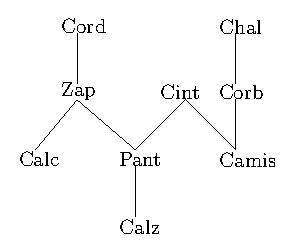
\includegraphics{diagH-tareas.eps}
\caption{Diagrama de Hasse para el orden de las tareas necesarias para vestirse}
\label{fig:diagH-tareas}
\end{figure}

En este caso, el diagrama nos entrega información como por ejemplo que lo primero que se debe hacer es ponerse los calcetines, los calzoncillos o la camisa, y que lo último que se hará será abrocharse los cordones, abrocharse el cinturón o ponerse el chaleco.
Los primeros son los elementos minimales del conjunto, los segundos son los elementos maximales del conjunto.
\end{ejemplo}

\begin{definicion}
Dado un orden parcial $(A,\preceq)$, un Diagrama de Hasse para él se construye siguiendo las reglas:
\begin{enumerate}
  \itemsep 0pt
  \item Para cada elemento $x\in A$, $x$ se debe ``dibujar en el digarama''.
  \item Si $x,y\in A$ dos elementos distintos tales que $x\preceq y$, entonces x debe dibujarse ``más abajo'' que $y$ en el diagrama.
  \item Si $x,y\in A$, $x\not=y$, $x\preceq y$ y no existe ningún elemento $z$ (distinto de $x$ e $y$) tal que $x\preceq z$ y $z\preceq y$, entonces se dibuja una linea entre $x$ e $y$ en el diagrama.
\end{enumerate}
\end{definicion}

\begin{ejemplo}
Sea $\U=\{1,2,3\}$ y el orden $(\P(\U),\subseteq)$.
Su diagrama de Hasse asociado se ve en la figura~\ref{fig:diagH-subconjuntos}.

\begin{figure}[h!]
\centering
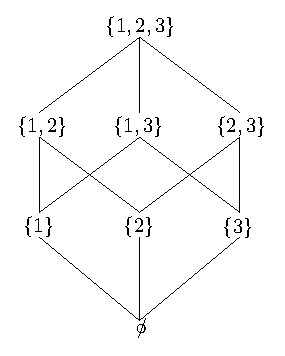
\includegraphics{diagH-subconjuntos}
\caption{Diagrama de Hasse para el orden $(\P(\{1,2,3\}),\subseteq)$.}
\label{fig:diagH-subconjuntos}
\end{figure}
\end{ejemplo}

\begin{definicion}
Sea $(A,\preceq)$ un orden parcial.
Si para cualquier par de elementos $x,y\in A$ ocurre que el conjunto $\{x,y\}\subseteq A$ tiene supremo e ínfimo en $A$, diremos que $(A,\preceq)$ es un \emph{reticulado}.
Llamaremos también \emph{reticulado} a su Diagrama de Hasse asociado.
\end{definicion}

\begin{ejemplo}
El orden $(\P(\{1,2,3\}),\subseteq)$ es un reticulado.
En general, para cualquier conjunto $\U$, el orden $(\P(\U),\subseteq)$ es un reticulado,
de hecho dados $A,B\in\P(\U)$, el conjunto $\{A,B\}$ siempre tiene supremo e ínfimo, a saber \[\sup\{A,B\}=A\cup B \hspace*{3em} \inf\{A,B\}=A\cap B.\]
La demostración de estas dos últimas propiedades se deja como ejercicio.
\end{ejemplo}


\subsection{Relaciones de Equivalencia y Particiones}
\begin{definicion}
Diremos que una relación binaria $R$ sobre un conjunto $A$ es una {\bf relación de equivalencia} si cumple con ser, refleja, simétrica y transitiva.
Generalmente cuando $R$ sea una relación de equivalencia sobre $A$, la denotaremos por el símbolo $\eqr$.
Si $(x,y)\in\eqr$ o equivalentemente si $x\eqr y$ diremos que ``$x$ es equivalente a $y$''.
\end{definicion}

\begin{ejemplo}
\begin{enumerate}
  \itemsep 0pt
  \item La relación de equivalencia módulo $n$, $\equiv_n$ sobre los naturales es una relación de equivalencia.
  \item La relación $R_C$ sobre $\P(\U)$ para un $\U$ cualquiera, tal que $A,B,C\in\P(\U)$, $A R_CB\Leftrightarrow A\cap C= B\cap C$ es una relación de equivalencia.
  \item La relación $\downarrow$ sobre $\N\times\N$ definida por $(m,n)\downarrow(r,s)\Leftrightarrow m+s=n+r$, es una relación de equivalencia.

\end{enumerate}
En la sección~\ref{sec:prop-rel} demostramos las propiedades necesarias para los casos 1 y 2.
La demostración de que $\downarrow$ es también una relación de equivalencia se deja como ejercicio.
\end{ejemplo}

\begin{definicion}
Sea $A$ un conjunto cualquiera, y sea $\mathcal S$ una colección de subconjuntos de $A$ ($\mathcal S\subseteq\P(A)$).
Diremos que $\mathcal S$ es una partición de $A$ si cumple:
\begin{enumerate}
  \itemsep 0pt
  \item $\forall X\in\mathcal S$, $X\not=\emptyset$.
  \item $\bigcup\mathcal S=A$
  \item $\forall X,Y\in\mathcal S$ si $X\not=Y$ entonces $X\cap Y=\emptyset$.
\end{enumerate}
Esta definición nos dice que una partición de $A$ es una colección de conjuntos no vacíos (1) disjuntos (3) y exhaustivos (2), es decir, una colección de conjuntos no vacíos, que no comparten elementos y tal que de su unión resulta el conjunto $A$ completo.
\end{definicion}

Existe una íntima relación entre las particiones de un conjunto y las relaciones de equivalencia sobre él.
La siguiente definición nos indica la primera de estas relaciones.

\begin{definicion}
Sea $\eqr$ una relación de equivalencia cualquiera sobre un conjunto $A$.
Para cada $x\in A$ se define \emph{la clase de equivalencia de} $x$ como el conjunto $[x]_\eqr$
\[
[x]_\eqr=\{y\in A\;|\; y\eqr x\}.
\]
Cuando la relación de equivalencia (en este caso $\eqr$) esté implícita en la aplicación, a veces en vez de $[x]_\eqr$ hablaremos simplemente de $[x]$.
Una de las primeras propiedades importantes que se deben notar es que, siempre ocurre que $x\in[x]$, y que si $x\eqr y$ entonces se cumple que $[x]=[y]$ >Por qué?
\end{definicion}

\begin{ejemplo}
Tomemos la relación $\equiv_4$ sobre los naturales.
Ya sabemos que esta es una relación de equivalencia, miremos cuáles son sus clases de equivalencia:
\[
\begin{array}{l}
[0]=\{0,4,8,12,16,\ldots\} \\
\text{[}1]=\{1,5,9,13,17,\ldots\} \\
\text{[}2]=\{2,6,10,14,18,\ldots\} \\
\text{[}3]=\{3,7,11,15,19,\ldots\} \\
\end{array}
\]
Las anteriores son todas las clases de equivalencias generadas por la relación $\equiv_4$, de hecho si tomamos por ejemplo $[4]$ sabemos que $[4]=[0]$ y que $[23]=[3]$.
\end{ejemplo}

\begin{ejemplo}
Tomemos la relación $\downarrow$ sobre $\N\times\N$, las clases de equivalencia generadas son:
\[
\begin{array}{rcl}
[(0,0)]& = &\{(0,0),(1,1),(2,2),\ldots\} \\
\text{[}(0,1)]& = &\{(0,1),(1,2),(2,3),\ldots\} \\%= \{(i,j)\;|\;i+1=j\} \\
\text{[}(1,0)]& = &\{(1,0),(2,1),(3,2),\ldots\} \\%= \{(i,j)\;|\;j+1=i\}\\
\text{[}(0,2)]& = &\{(0,2),(1,3),(2,4),\ldots\} \\%= \{(i,j)\;|\;i+2=j\} \\
\text{[}(2,0)]& = &\{(2,0),(3,1),(4,2),\ldots\} \\%= \{(i,j)\;|\;j+2=i\}\\
&\vdots\\
\text{[}(0,n)]& = &\{(0,n),(1,n+1),(2,n+2),\ldots\} \\% = \{(i,j)\;|\;i+n=j\}\\
\text{[}(n,0)]& = &\{(n,0),(n+1,1),(n+2,2),\ldots\} \\%= \{(i,j)\;|\;j+n=i\}\\
&\vdots
\end{array}
\]
\vspace*{-25pt}
\end{ejemplo}


\begin{teorema}
\label{teo:equiv-rel}
Sea $\eqr$ una relación de equivalencia sobre un conjunto $A$, entonces se cumple que
\begin{enumerate}
  \itemsep 0pt
  \item $\forall x\in A$, $x\in[x]$.
  \item $x\eqr y$ si y sólo si $[x]=[y]$.
  \item si $[x]\not=[y]$ entonces $[x]\cap[y]=\emptyset$.
\end{enumerate}
\begin{demostracion}
Las primeras dos propiedades se dejan como ejercicio, demostraremos sólo la propiedad 3.
\begin{enumerate}
  \setcounter{enumi}{2}
  \item Daremos un argumento por contradicción.
  Supongamos que $[x]\not=[y]$, y supongamos que $[x]\cap[y]\not=\emptyset$, entonces necesariamente existe un $z$ tal que $z\in[x]$ y $z\in[y]$.
  Esto quiere decir que simultáneamente ocurre que $z\eqr x$ y que $z\eqr y$.
  Dado que $\eqr$ es una relación de equivalencia, cumple con ser simétrica y transitiva.
  Usando la primera de estas propiedades concluimos que $x\eqr z$ y usando esto último y la propiedad de transitividad concluimos que $x\eqr y$, luego por la porpiedad (2) se concluye que $[x]=[y]$ lo que es una contradicción.
\end{enumerate}
\end{demostracion}

De este teorema se concluye inmediatamente el siguiente.
\end{teorema}

\begin{teorema}
\label{teo:clases-equiv}
Sea $\eqr$ una relación de equivalencia sobre un conjunto $A$.
Y sea $\mathcal S$ el conjunto de las clases de equivalencia de $\eqr$, o sea $\mathcal S=\{[x]\;|\;x\in A\}$.
Entonces $S$ forma una partición de $A$.

\begin{demostracion}
Debemos demostrar las tres propiedades necesarias para que $\mathcal S$ sea una partición, a saber, que (1) es una colección de conjuntos no vacíos, (2) exhaustivos y (3) disjuntos.
En este caso, cada uno de los conjuntos de $\mathcal S$ son las clases de equivalencia de $\eqr$.
\begin{enumerate}
  \vspace*{-\topsep}
  \itemsep 0pt
  \item Debemos demostrar que $\forall X\in\mathcal S$, se tiene que $X\not=\emptyset$.
  Ahora, como los elementos de $\mathcal S$ son clases de equivalencia de $\eqr$ y dado que para todo $x$ se cumple que $x\in[x]\Rightarrow [x]\not=\emptyset$ (parte 1 del teorema~\ref{teo:equiv-rel}) entonces todos los conjuntos de $\mathcal S$ son distintos de vacío.
  \item Debemos demostrar que $\bigcup\mathcal S=A$.
  Es claro que $\bigcup\mathcal S\subseteq A$ ya que un elemento pertenece a $\bigcup\mathcal S$ si  pertenece a alguna de las clases de equivalencia de $\eqr$, y en las clases de equivalencia de $\eqr$ sólo hay elementos de $A$.
  Sólo falta demostrar entonces que $A\subseteq\bigcup\mathcal S$.
  Sea $x\in A$ sabemos que $x\in[x]$ y dado que $[x]\in\mathcal S$ concluimos que $x\in\bigcup\mathcal S$.
  \item Debemos demostrar que si $X,Y\in\mathcal S$ y $X\not=Y$ entonces $X\cap Y=\emptyset$.
  Dado que los conjuntos en $\mathcal S$ son clases de equivalencia, y por la propiedad 3 del teorema~\ref{teo:equiv-rel}, tenemos que $[x]\not=[y]$ entonces $[x]\cap[y]=\emptyset$ que es lo que queríamos demostrar.
\end{enumerate}
\end{demostracion}
\end{teorema}

\begin{definicion}
Al conjunto $\mathcal S$ del teorema anterior le llamaremos \emph{conjunto cuociente} de $A$ con respecto a $\eqr$ y lo anotaremos $A/\eqr$,
\[
A/\eqr=\{[x]\;|\;x\in A\}
\]
El teorema~\ref{teo:clases-equiv} dice entonces que si $\eqr$ es una relación de equivalencia sobre $A$, el conjunto cuociente $A/\eqr$ forma una partición de $A$.

Definiremos además el \emph{índice} de una relación de equivalencia como la cantidad de clases de equivalencias que induce, es decir, como la cantidad de elementos del conjunto cuociente $A/\eqr$.
\end{definicion}

\begin{ejemplo}
Para la relación $\equiv_4$ sobre los naturales, se tiene que el conjunto cuociente es:
\[
\begin{array}{rl}
\N/\equiv_4&=\{\{0,4,8,\ldots\},\{1,5,9,\ldots\},\{2,6,10,\ldots\},\{3,7,11,\ldots\}\} \\
&=\{[0],[1],[2],[3]\}
\end{array}
\]
El índice de la relación $\equiv_4$ sobre $\N$ es $4$ ya que induce $4$ clases de equivalencias distintas.

Para la relación $\downarrow$ sobre $\N\times\N$, se tiene que el conjunto cuociente es:
\[
(\N\times\N)/\downarrow=\{[(0,0)],[(0,1)],[(1,0)],[(0,2)],[(2,0)],[(0,3)],\ldots\}
\]
Esta relación tiene índice infinito ya que induce una cantidad infinita de clases de equivalencia.
Un diagrama de las particiones inducidas por esta relación se puede ver en la figura~\ref{fig:uparrow-equiv}.
\begin{figure}[h!]
\centering
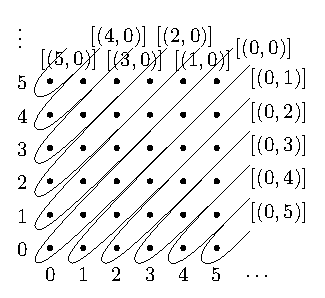
\includegraphics{uparrow-equiv}
\caption{Partición de $\N\times\N$ inducida por la clase de equivalencias $\downarrow$.}
\label{fig:uparrow-equiv}
\end{figure}
\end{ejemplo}

Algo muy interesante es que a partir de una partición cualquiera de un conjunto siempre se forma una relación de equivalencia.
El siguiente teorema lo establece.

\begin{teorema}
Sea $\mathcal S$ una partición cualquiera sobre un conjunto $A$, entonces la relación $\eqr$ definida como sigue es una relación de equivalencia sobre $A$.
\[
x,y\in A,\;\;\;\;\; x\eqr y\Leftrightarrow \exists X\in\mathcal S\text{ tal que }\{x,y\}\subseteq X,
\]
o sea, $x$ está relacionado con $y$ cuando ambos pertenecen al mismo conjunto en $\mathcal S$.

\begin{demostracion}
Sólo se debe comprobar que $\eqr$ es refleja, simétrica y transitiva.
Se deja como ejercicio.
\end{demostracion}

En este caso también se cumple que $\mathcal S=A/\eqr$.
\end{teorema}

Uno de las mayores aplicaciones de las relaciones de equivalencia es que estas pueden usarse para definir nuevos conjuntos a partir del conjunto cuociente.
Veremos dos ejemplos de cómo a partir de un conjunto conocido ($\N$) pueden crearse nuevos conjuntos y definirse operaciones sobre los elementos de los nuevos conjuntos.

\begin{ejemplo}
Podemos definir el conjunto de los naturales módulo $4$, $\N_4$, como el conjunto cuociente $\N/\equiv_4$, así $\N_4=\{[0],[1],[2],[3]\}$.
Lo interesante es que podemos definir operadores en este nuevo conjunto a partir de operadores en el antiguo conjunto.
Definimos la suma módulo $4$ de la siguiente forma:
\[
[i]+_{(4)}[j]=[i+j].
\]
Así por ejemplo $[3]+_{(4)}[2]=[3+2]=[5]=[1]$, de la misma forma $[1]+_{(4)}[3]=[0]$.
También podemos definir la multiplicación módulo $4$ de la siguiente manera:
\[
[i]\cdot_{(4)}[j]=[i\cdot j].
\]
Así por ejemplo $[2]\cdot_{(4)}[3]=[2\cdot 3]=[6]=[2]$, de la misma forma $[3]\cdot_{(4)}[3]=[1]$.

Si damos un paso más y renombramos los elementos de $\N_4$ de la siguiente manera:
%manera tal que a $[0]$ le llamamos simplemente $0$, a $[1]$ le llamamos $1$, a $[2]$ le llamamos $2$, y a $[3]$ le llamamos $3$,  
\[
\begin{array}{ccc}
[0]&\leftrightarrow&0\\
\text{[} 1]&\leftrightarrow&1\\
\text{[}2]&\leftrightarrow&2\\
\text{[}3]&\leftrightarrow&3
\end{array}
\]
o sea, a $[0]$ le llamamos simplemente $0$, a $[1]$ le llamamos $1$, etc., y además reemplazamos el símbolo $+_{(4)}$ por $+$, y $\cdot_{(4)}$ por $\cdot$, tenemos un conjunto con una nueva estructura de operadores:
\[
\N_4=\{0,1,2,3\}\text{ con operadores }+\text{ y }\cdot
\]
tal que por ejemplo, $2+2=0$, $3+2=1$, $3\cdot 3=1$, $2\cdot 1=2$, etc.
\end{ejemplo}

\begin{ejemplo}
Formalmente podemos definir al conjunto de los números enteros $\Z$ como el conjunto cuociente $(\N\times\N)/\downarrow$, así formalmente $\Z=\{[(0,0)],[(0,1)],[(1,0)],[(0,2)],[(2,0)],[(0,3)],\ldots\}$.
Intuitivamente la clase de equivalencia $[(0,i)]$ está representando al entero $i$, y la clase de equivalencia $[(i,0)]$ está representando al entero $-i$.
Entonces podemos renombrar los elementos de este conjunto de la siguiente manera:
\[
\begin{array}{ccr}
\text{[}(0,0)]&\leftrightarrow&0\\
\text{[}(0,1)]&\leftrightarrow&1\\
\text{[}(1,0)]&\leftrightarrow&-1\\
\text{[}(0,2)]&\leftrightarrow&2\\
\text{[}(2,0)]&\leftrightarrow&-2\\
\text{[}(0,3)]&\leftrightarrow&3\\
&\vdots
\end{array}
\]
luego $\Z=\{0,1,-1,2,-2,3,-3,4\ldots\}$.
Lo primero (importante) que notar es que ``$-1$'' es {\bf simplemente un nombre} que se le da a la clase $[(1,0)]$, así como ``$-2$'' a la clase $[(2,0)]$, no debe interpretarse el símbolo ``$-$'' con ningún significado especial, de hecho en nuestro caso ``$-$'' no significa nada por sí sólo.

Podemos intentar definir operadores sobre este nuevo conjunto de manera similar al ejemplo anterior, teniendo la intuición de que estos deben captar la estructura de $\Z$.
Por ejemplo podríamos definir el operador $+_\downarrow$ de la siguiente forma:
\[
[(m,n)]+_\downarrow[(r,s)]=[(m+r,n+s)],
\]
así se tendría que $[(0,7)]+_\downarrow[(5,0)]=[(5,7)]=[(0,2)]$, que $[(18,0)]+_\downarrow[(0,4)]=[(18,4)]=[(14,0)]$, y que $[(3,0)]+_\downarrow[(6,0)]=[(9,0)]$, etc.,
lo que capta completamente la idea de la suma entera, de hecho resulta que $7+_\downarrow-5=2$, $-18+_\downarrow 4=-14$ y $-3+_\downarrow-6=-9$.

Para definir la multiplicación debemos cuidarnos un poco más, de hecho una definición como la siguiente no nos lleva a buen término
\[
[(m,n)]\cdot_\downarrow[(r,s)]=[(m\cdot r,n\cdot s)],
\]
ya que por ejemplo nos resulta que $[(3,0)]\cdot_\downarrow[(4,0)]=[(3\cdot 4,0\cdot 0)]=[(12,0)]$ o sea que $-3\cdot_\downarrow-4=-12$ cuando quisiéramos que el resultado fuese $12$.
La definición correcta de $\cdot_\downarrow$ es:
\[
[(m,n)]\cdot_\downarrow[(r,s)]=[(m\cdot s+n\cdot r,m\cdot r+n\cdot s)].
\]
De hecho ahora resulta que $[(3,0)]\cdot_\downarrow[(4,0)]=[(3\cdot 0+0\cdot 4,3\cdot 4+0\cdot 0)]=[(0,12)]$, y que $[(0,3)]\cdot_\downarrow[(0,3)]=[(0\cdot 3+3\cdot 0,0\cdot 0+3\cdot 3)]=[(0,9)]$, etc., lo que capta la idea de multiplicación entera ya que $-3\cdot_\downarrow-4=12$ y $3\cdot_\downarrow 3=9$.

Luego podemos usar el conjunto $\Z=\{0,1,-1,2,-2,3,\ldots\}$ y renombrar las operaciones $+_\downarrow$ y $\cdot_\downarrow$ como $+$ y $\cdot$ simplemente para obtener a los enteros y sus dos operaciones habituales.
\end{ejemplo}

\newpage
\section{Lógica de Predicados de Primer Órden***}

[***falta completar***]

\newpage
\section{Funciones y Cardinalidad}
En esta sección nos dedicaremos principalmente al problema de cómo establecer el tamaño de un conjunto, la cantidad de elementos que el conjunto tiene.
El tema puede parecer trivial a simple vista, por ejemplo, todos sabemos que el siguiente conjunto
\[
A=\{a,b,c,d,e,f\}
\]
tiene $6$ elementos, cómo lo sabemos, simplemente \emph{contamos} los elementos.
Cuando contamos los elementos del conjunto $A$ por ejemplo, establecemos una \emph{correspondencia} como la siguiente:
\[
\begin{array}{ccc}
a&\rightarrow&1\\
b&\rightarrow&2\\
c&\rightarrow&3\\
d&\rightarrow&4\\
e&\rightarrow&5\\
f&\rightarrow&6\\
\end{array}
\]
de la cual concluimos que la cantidad de elementos es $6$.
La noción de \emph{contar} es muy intuitiva y simple de aplicar cuando los conjuntos son finitos, pero >cómo contamos los elementos de un conjunto infinito?
Veremos que podemos extender esta noción de \emph{correspondencia} para conjuntos que no necesariamente son finitos.
Comenzaremos nuestro estudio con el concepto de función.

\subsection{Funciones}
\begin{definicion}
Sea $f$ una relación binaria de un conjunto $A$ en un conjunto $B$, $f\subseteq A\times B$, $f$ es una función de $A$ en $B$ si dado cualquier elemento $a\in A$ existe un único elemento $b\in B$ tal que $afb$, en símbolos
\[
afb \wedge afc \;\;\Rightarrow\;\; b=c.
\]

Sea $a\in A$, para denotar al único elemento de $B$ que está relacionado con $a$ escribimos $f(a)$, así, si $afb$ entonces escribimos $b=f(a)$.
Si $b=f(a)$, a $b$ se le llama \emph{imagen} de $a$, y a $a$ se le llama \emph{preimagen} de $b$.
Cuando $f$ sea función de $A$ en $B$ escribiremos:
\[
\begin{array}{rrcl}
f:& A&\rightarrow &B\\
& a&\rightarrow &f(a)
\end{array}
\]
Una función $f:A\rightarrow B$ se dice \emph{total}, si todo elemento en $A$ tiene imagen, o sea, si para todo $a\in A$ existe un $b\in B$ tal que $b=f(a)$.
Una función que no sea total se llama \emph{parcial}.
Cuando nosotros hablemos de función nos referiremos a función total, a menos que se diga lo contrario.
\end{definicion}

\begin{ejemplo}
Las siguientes relaciones son todas funciones (totales) 
de $\{0,1,2,3\}$ en $\{0,1,2,3\}$:
\[
\begin{array}{l}
f_1=\{(0,0),(1,1),(2,2),(3,3)\} \\
f_2=\{(0,1),(1,1),(2,1),(3,1)\} \\
f_3=\{(0,3),(1,2),(2,1),(3,0)\} \\
\end{array}
\]
>Cuántas funciones (totales) 
distintas de $\{0,1,2,3\}$ en $\{0,1,2,3\}$ podemos construir?
Exactamente 256, >por qué?.
\end{ejemplo}

\begin{ejemplo}
Las funciones también pueden definirse usando expresiones que dado un $x$ muestren cómo obtener $f(x)$, por ejemplo las siguientes son definiciones para funciones de $\R$ en $\R$.
\[
\begin{array}{l}
\forall x\in\R,\;\; f_1(x)=x^2+1\\
\forall x\in\R,\;\; f_2(x)=\lfloor x+\sqrt{x}\rfloor\\
\forall x\in\R,\;\; f_3(x)=0 \\
\forall x\in\R,\;\; f_4(x)=\left\{
														\begin{array}{rr}
														1 & \text{si }x\geq 0\\
														-1 & \text{si }x<0
														\end{array}
														\right.
\end{array}
\]
\end{ejemplo}

\begin{ejemplo}
Sea $A$ un conjunto cualquiera, las siguientes son funciones de $A$ en $\P(A)$.
\[
\begin{array}{l}
\forall a\in A,\;\; f_1(a)=\{a\} \\
\forall a\in A,\;\; f_2(a)=A-\{a\} \\
\forall a\in A,\;\; f_3(a)=\emptyset
\end{array}
\]
\end{ejemplo}

\begin{definicion}
Diremos que una función $f:A\rightarrow B$ es:
\begin{enumerate}
  \item Inyectiva (o 1-1) si para cada par de elementos $x,y$ ocurre que $f(x)=f(y)\Rightarrow x=y$ (o equivalentemente $x\not=y\Rightarrow f(x)\not=f(y)$), es decir no existen dos elementos distintos en $A$ con la misma imagen.
  \item Sobreyectiva (o simplemente sobre) si cada elemento en $b\in B$ tiene una preimagen en $a\in A$, o sea, $\forall b\in B\;\;\exists a\in A$ tal que $f(a)=b$.
  \item Biyectiva si es al mismo tiempo inyectiva y sobreyectiva.
\end{enumerate}
\end{definicion}

\begin{ejemplo}
A continuación se listan funciones y las propiedades que cumplen (o no cumplen):
\begin{enumerate}
  \itemsep 0pt
  \item $f:A\rightarrow\P(A)$, $\forall a\in A$ $f(a)=\{a\}$, es inyectiva y no sobreyectiva.
  \item $f:A\rightarrow\P(A)$, $\forall a\in A$ $f(a)=\emptyset$, ni inyectiva ni sobreyectiva.
  \item $f:\N\rightarrow\{0,1,2,3\}$, $\forall n\in\N$ $f(n)=n\mod 4$, es sobreyectiva y no inyectiva.
  \item $f:\{0,1,2,3\}\rightarrow\{0,1,2,3\}$, $f(n)=n+2\mod 4$, es biyectiva.
\end{enumerate}
\end{ejemplo}

Una propiedad muy interesante de las funciones y los conjuntos finitos es la siguiente:

\begin{teorema}[Principio de los Cajones (o del Palomar).]
Suponga que se tienen $m$ pelotas y $n$ cajones y que $m>n$, entonces, después de repartir las $m$ pelotas en los $n$ cajones, necesariamente existirá un cajón con más de una pelota.

En lenguaje matemático, si se tiene una función $f:\{0,1,\ldots,m-1\}\rightarrow\{0,1,\ldots,n-1\}$ con $m>n$, la función $f$ no puede ser inyectiva, es decir, necesariamente existirán $x,y\in\{0,1,\ldots,m-1\}$ tales que $x\not=y$ y $f(x)=f(y)$.

Se puede establecer un principio similar pero con respecto a la sobreyectividad de $f$, si $f:\{0,1,\ldots,m-1\}\rightarrow\{0,1,\ldots,n-1\}$ con $m<n$, entonces $f$ no puede ser sobreyectiva.

Agrupando las observaciones anteriores podemos establecer lo siguiente: la única forma de que una función $f:\{0,1,\ldots,m-1\}\rightarrow\{0,1,\ldots,n-1\}$ sea biyectiva (inyectiva y sobreyectiva al mismo tiempo), es que $m=n$.
\end{teorema}

\begin{ejemplo}
Si en una habitación hay 8 personas, entonces necesariamente existen dos de ellas que este año celebran su cumpleaños el mismo día de la semana.
Las 8 personas las podemos modelar como el conjunto $P=\{0,1,\ldots,7\}$ y los días de la semana como el conjunto $S=\{0,1,2\ldots,6\}$. 
El día de la semana que se celebra el cumpleaños de cada unas resulta ser una función de $P$ en $S$, por el principio de los cajones, esta función no puede ser inyectiva, luego al menos dos personas distintas celebrarán su cumpleaños el mismo día de la semana.
\end{ejemplo}

Este principio es sumamente intuitivo, sin embargo resulta de gran utilidad cuando se trabaja con conjuntos finitos, en el contexto de computación cuando se trabaja por ejemplo con estructuras de datos como arreglos, tablas de hash, grafos, etc.

\subsection{Cardinalidad}
La \emph{cardinalidad} de un conjunto es una medida de la cantidad de elementos que posee.
Ahora que manejamos el concepto de función, podemos formalizar la noción de cantidad de elementos de un conjunto.

\begin{definicion}
Sean $A$ y $B$ dos conjuntos cualesquiera, diremos que ``$A$ es equinumeroso con $B$'' o que ``$A$ tiene el mismo tamaño que $B$'', y escribiremos $A\eqr B$, si existe una función biyectiva entre $A$ y $B$.
\[
A\eqr B\;\;\;\Leftrightarrow\;\;\;\exists f:A\rightarrow B,\;\;f\text{ función biyectiva.}
\]
Nuestra definición dice que $A$ y $B$ tienen el mismo tamaño, si los elementos de $A$ se pueden poner en correspondencia con los elementos de $B$.
Note que $\eqr$ es una relación definida sobre el universo de los conjuntos. 
No es difícil notar que $\eqr$ cumple con ser refleja, simétrica y transitiva, y por lo tanto es una relación de equivalencia.
\begin{itemize}
  \itemsep 0pt
  \item refleja: $f:A\rightarrow A$ tal que $f(a)=a$ $\forall a\in A$ es una función biyectiva, por lo que $A\eqr A$.
  \item simétrica: si $A\eqr B$ $\Rightarrow$ existe $f:A\rightarrow B$ biyectiva, entonces la relación $f^{-1}:B\rightarrow A$ es también biyectiva y por lo tanto $B\eqr A$.
  \item transitiva: si $A\eqr B$ y $B\eqr C$ $\Rightarrow$ existen $f:A\rightarrow B$ y $g:B\rightarrow C$ biyectivas, luego $f\circ g:A\rightarrow C$ (la composición de las funciones) es una función biyectiva, por lo que $A\eqr C$.
\end{itemize}
Dado que $\eqr$ es una relación de equivalencia, podemos tomar las clases de equivalencia inducidas por esta relación.
A la clase de equivalencia de un conjunto $A$ le llamaremos \emph{cardinalidad} de $A$ y la anotaremos por $|A|$.
Así si $A$ es equinumeroso con $B$, se cumple que $|A|=|B|$.
\end{definicion}


\subsubsection*{Conjuntos Finitos}
Diremos que $A$ es un conjunto finito si $A\eqr\{0,1,2,\ldots,n-1\}$ para algún $n\in\N$, es decir, si existe una función biyectiva $f:A\rightarrow\{0,1,2,\ldots,n-1\}$.
Si $A\eqr\{0,1,2,\ldots,n-1\}$ ``llamaremos'' $n$ a la cardinalidad de $A$, o sea $|A|=n$, y diremos que $A$ tiene $n$ elementos.
Un caso especial es cuando $A=\emptyset$, en este caso $|A|=0$, de hecho, el único conjunto con cardinalidad $0$ es $\emptyset$.
Si $A$ no es un conjunto finito diremos entonces que es un conjunto infinito.

\begin{ejemplo}
Ahora si podemos decir con autoridad que $A=\{a,b,c,d,e,f\}$ tiene $6$ elementos, o que $|A|=6$, de hecho la siguiente es una función biyectiva entre $A$ y $\{0,1,2,3,4,5\}$
\[
\begin{array}{ccc}
&f\\
a&\rightarrow&0\\
b&\rightarrow&1\\
c&\rightarrow&2\\
d&\rightarrow&3\\
e&\rightarrow&4\\
f&\rightarrow&5\\
\end{array}
\]
\end{ejemplo}

El siguiente teorema nos entrega una relación entre $|A|$ y $|\P(A)|$ para conjuntos $A$ finitos, antes veremos un lema muy simple:

\begin{lema}
Sean $A$ y $B$ dos conjuntos finitos tales que $A\cap B=\emptyset$.
Entonces $|A\cup B|=|A|+|B|$.

\begin{demostracion}
Supongamos que $|A|=n$ y que $|B|=m$.
Sabemos entonces que $A\eqr\{0,1,\ldots n-1\}$ y que $B\eqr\{0,1,\ldots,m-1\}$, luego existen funciones biyectivas $f:A\rightarrow\{0,1,\ldots n-1\}$ y $g:B\rightarrow\{0,1,\ldots,m-1\}$.
Sea $h:(A\cup B)\rightarrow\{0,1,\ldots,n,n+1,\ldots,n+m-1\}$ tal que
\[
h(x)=\left\{\begin{array}{lr}
			f(x)&\text{si }x\in A \\
			n+g(x)&\text{si }x\in B
			\end{array}\right.
\]
Primero se debe notar que $h$ está bien definida como función ya que no existe un $x$ que pertenezca simultáneamente a $A$ y $B$.
No es difícil notar también que $h$ es biyectiva por lo que se concluye que $|A\cup B|=n+m=|A|+|B|$.

Demostraremos la biyectividad de $h$ sólo como un ejemplo de este tipo de demostraciones.
Para demostrar biyectividad se debe establecer las propiedades de sobreyectividad e inyectividad.
Para establecer la sobreyectividad de $h$ debemos demostrar que $\forall k\in\{0,1,\ldots,n,n+1,\ldots,n+m-1\}$ existe un $x\in A\cup B$ tal que $k=h(x)$.
La demostración la podemos hacer por casos: si $k<n$ entonces dado que $f$ es sobreyectiva en $\{0,1,\ldots,n-1\}$ sabemos que existe un $x\in A$ tal que $k=f(x)=h(x)$, si $n\leq k<n+m$ entonces dado que $g$ es sobreyectiva en $\{0,1,\ldots,m-1\}$ sabemos que existe un $x\in B$ tal que $g(x)=k-n$ y por lo tanto $k=n+g(x)=h(x)$, finalmente $h$ es sobreyectiva en $\{0,1,\ldots,n,n+1,\ldots,n+m-1\}$.
Para establecer la inyectividad de $h$ debemos demostrar que si $h(x)=h(y)$ entonces necesariamente $x=y$.
Otra vez podemos trabajar por casos: si $h(x)=h(y)<n$ entonces necesariamente $h(x)=f(x)=h(y)=f(y)$ de donde se concluye que $f(x)=f(y)$ y dado que $f$ es inyectiva obtenemos que $x=y$, si en cambio $n\leq h(x)=h(y)<n+m$ sabemos que $h(x)=n+g(x)=h(y)=n+g(y)$ de donde se concluye que $g(x)=g(y)$ y dado que $g$ es inyectiva obtenemos que $x=y$, finalmente $h$ es iyectiva.
\end{demostracion}
\end{lema}

\begin{teorema} 
Sea $A$ un conjunto finito, entonces $|\P(A)|=2^{|A|}$.

\begin{demostracion}
La demostración se hará por inducción en la cardinalidad de $A$.
\begin{inducciondemo}
  \BI Si $|A|=0$ entonces $A=\emptyset$ $\Rightarrow$ $\P(A)=\{\emptyset\}\eqr\{0\}$ por lo tanto $|\P(A)|=1=2^0=2^{|A|}$.
  \HI Supongamos que para cualquier conjunto $A$ tal que $|A|=n$ se cumple que $|\P(A)|=2^n=2^{|A|}$.
  \TI Sea $A$ un conjunto tal que $|A|=n+1$, y sea $B=A-\{a\}$, con $a$ un elemento cualquiera de $A$.
  El conjunto $B$ cumple con $|B|=n$,\footnote{En estricto rigor, para establecer que $|B|=n$ se debería mostrar una función biyectiva de $B$ en $\{0,1,\ldots,n\}$, hacemos el paso rápido apelando a la intuición.} por lo que $|\P(B)|=2^n$.
  >Cómo podemos a partir de $\P(B)$ formar $\P(A)$?
  Si nos damos cuenta en $\P(B)$ están todos los subconjuntos de $B$, es decir, todos los subconjuntos de $A$ que no contienen el elemento $a$.
  Si llamamos $\mathcal A$ al conjunto
  \[
  \mathcal A=\{X\;|\;X\subseteq A\wedge a\in X\},
  \]
  es decir $\mathcal A$ está formado por todos los subconjuntos de $A$ que {\bf sí} contienen a $a$, no es difícil notar que $\mathcal A\cap\P(B)=\emptyset$ y que $\P(A)=\P(B)\cup\mathcal A$.
  Ahora, la siguiente función $f:\P(B)\rightarrow\mathcal A$ tal que $f(X)=X\cup\{a\}$, es una función biyectiva de $\P(B)$ en $\mathcal A$, por lo que concluimos que $\P(B)\eqr\mathcal A$ y por lo tanto $|\P(B)|=|\mathcal A|$.
  Luego, dado que $\mathcal A\cap\P(B)=\emptyset$ y que $\P(A)=\P(B)\cup\mathcal A$ y usando el lema anterior concluimos que 
  \[
  |\P(A)|=|\P(B)\cup\mathcal A|=|\P(B)|+|\mathcal A|=|\P(B)|+|\P(B)|=2^n+2^n=2^{n+1}=2^{|A|}.
  \]
\end{inducciondemo}
\end{demostracion}
\end{teorema}

Este último teorema implica que si $A$ es un conjunto finito, entonces la cardinalidad de $A$, es {\bf estrictamente menor} que la de $\P(A)$.

\subsubsection*{Conjuntos Infinitos}
La noción de cardinalidad de conjuntos finitos resulta ser bastante intuitiva, pero >qué pasa cuando los conjuntos son infinitos? >cómo comparo la cantidad de elementos de dos conjuntos infinitos?.

Tomemos el siguiente ejemplo, sea $\N$ el conjunto de todos los naturales y $\mathbb P=\{2k\;|\;k\in\N\}$ el conjunto de todos los naturales pares.
>Cuál es más grande $\N$ o $\mathbb P$?
Nuestra primera respuesta intuitiva: $\mathbb P$ es un subconjunto propio de $\N$, $\mathbb P\subset\N$ por lo que $\N$ es más grande.
Este razonamiento es correcto en el caso de conjuntos finitos...
>Qué pasa si aplicamos nuestra definición de cardinalidad?
Hemos definido que dos conjuntos son equinumerosos, o sea tienen la misma cantidad de elementos, si existe una función biyectiva de uno en el otro.
La función $f(n)=2n$ le asigna a cada natural un número par de la siguiente forma:
\[
\begin{array}{ccccccccccccccc}
0 & 1 & 2 & 3 & \cdots & n & n+1 & \cdots \\
\downarrow&\downarrow&\downarrow&\downarrow&\cdots&\downarrow&\downarrow&\cdots\\
0 & 2 & 4 & 6 & \cdots & 2n & 2n+2 & \cdots
\end{array}
\]
Esta es una función que ha puesto en correspondencia cada número natural con un número par, es una función biyectiva entre $\N$ y $\mathbb P$, luego $|\N|=|\mathbb P|$, o sea, <~<~existen las misma cantidad de números pares que naturales~!~!
No es difícil notar que pasará lo mismo con el conjunto $\mathbb I$ de los números impares, de hecho $|\N|=|\mathbb P|=|\mathbb I|$.
Esta discusión motiva nuestra siguiente definición.

\begin{definicion}
Un conjunto $A$ se dice enumerable si $|A|=|\N|$.
%La primera observación es que para que $A$ sea enumerable necesita ser infinito (>será verdad la implicación inversa?).
\end{definicion}

\begin{teorema}
Los conjuntos $\mathbb P$, $\mathbb I$ y $\Z$ son todos conjuntos enumerables.

\begin{demostracion}
Para demostrar esto, se deben exhibir funciones biyectivas desde $\N$ a cada uno de los conjuntos.
Para $\P$ la función $f(n)=2n$ es biyectiva, para $\mathbb I$ la función $f(n)=2n+1$ es biyectiva.
Para $\Z$ puede resultar un poco más complicado.
Tenemos que encontrar una forma de enviar cada natural con un entero, de manera tal de recorrer todos los enteros.
Una posible idea es enviar los naturales pares a los enteros positivos y los naturales impares a los enteros negativos de la siguiente forma:
\[
\begin{array}{ccccccccccccccc}
0 & 1 & 2 & 3 & 4 & \cdots & 2n & 2n+1 & \cdots \\
\downarrow&\downarrow&\downarrow&\downarrow&\downarrow&\cdots&\downarrow&\downarrow&\cdots\\
0 & -1 & 1 & -2 & 2 & \cdots & n & -(n+1) & \cdots
\end{array}
\]
La función sería la siguiente
\[
f(n)=\left\{\begin{array}{cr}
		\frac{n}{2}&\text{ si }n\text{ es par} \\
		-\frac{n+1}{2}&\text{ si }n\text{ es impar}
		\end{array}\right.
\]
que es biyectiva de $\N$ en $\Z$, y por lo tanto $|\N|=|\Z|$.
\end{demostracion}
\end{teorema}

Una manera de caracterizar a los conjuntos infinitos enumerables es mediante la siguiente definición:

\begin{definicion}[(Alternativa)]
Un conjunto $A$ es enumerable si y sólo si todos sus elementos se pueden poner en una lista infinita, o sea si 
\[
A=\{a_0,a_1,a_2,\ldots\}
\]
en otras palabras, si existe una sucesión infinita
\[
(a_0,a_1,a_2,\ldots,a_n,a_{n+1},\ldots)
\]
tal que \emph{todos} los elementos de $A$ aparecen en la sucesión \emph{una única vez} cada uno.
Si existe tal sucesión, la biyección entre $\N$ y $A$ es sumamente simple: $f(n)=a_n$.
\end{definicion}

Desde un punto de vista ``computacional'' podr\'{i}amos usar un programa en JAVA (o C, o C++, o Pascal, o cualquier lenguaje) para demostrar que un conjunto $A$ es enumerable. Si es posible implementar un programa $P$
que imprima sólo elementos de $A$ y tal que para cualquier $a\in A$ si esperamos lo suficiente, $P$ imprimirá $a$,
entonces $A$ es un conjunto enumerable (se debe suponer de todas maneras, que $P$ no tiene limitaciones de espacio, o sea, que puede usar variables de tamaño arbitrariamente grande).
Esto motiva la siguiente definición.

\begin{definicion}
Un conjunto $A$ es \emph{computacionalmente enumerable} si $A$ es infinito y existe un programa $P$ tal que todos los elementos de $A$ aparecen en el output de $P$ (separados por algún símbolo especial definido de antemano).
\end{definicion}

Note que la definición no exige que los elementos aparezcan una vez cada uno en el output, pero sí que todos aparezcan en algún momento.
Un punto ``interesante'' en la definición anterior (y que veremos más adelante) es que hay conjuntos enumerables que no son computacionalmente enumerables. O sea, existen conjuntos que pueden ponerse en una lista infinita, pero que no pueden ser puestos en esta lista por un computador.


La anterior definición nos sirve para demostrar el siguiente teorema.

\begin{teorema}
Los conjuntos $\Q$ y $\N\times\N$ son también enumerables, o sea $|\Q|=|\N|$ y $|\N\times\N|=|\N|$.

\begin{demostracion}
A primera vista pareciera imposible que $|\Q|=|\N|$ (que la cantidad de racionales sea igual a la cantidad de naturales) ya que entre cualquier par de naturales existe una cantidad infinita de racionales, más aún, entre cualquier par de racionales existe otro racional.
Sin embargo nuestra intuición no es de mucha utilidad en el caso infinito, debemos aplicar nuestra definición de ser enumerable.

Para mostrar que un conjunto es enumerable, basta argumentar que todos sus elementos se pueden poner en una lista infinita que los contenga a todos.
Partiremos por poner a $\N\times\N$ en una lista infinita.
Nuestra primera aproximación podría ser una sucesión de este tipo:
\[
((0,0),(0,1),(0,2),\ldots,(0,n),(0,n+1),\ldots).
\]
El problema de esta organización es que, a pesar de que los elementos se encuentran en una lista, no todos los elementos de $\N\times\N$ aparecen en ella.
Esta claro que una sucesión del tipo $((0,0),(1,0),(2,0),\ldots)$ tampoco funciona.
La clave para organizar a $\N\times\N$ en una lista está en encontrar una forma de recorrer la siguiente matriz infinita:
\[
\left\lceil
\begin{array}{ccccccccc}
(0,0) & (0,1) & (0,2) & (0,3) & \cdots\\
(1,0) & (1,1) & (1,2) & (1,3) & \cdots\\
(2,0) & (2,1) & (2,2) & (2,3) & \cdots\\
(3,0) & (3,1) & (3,2) & (3,3) & \cdots\\
\vdots&\vdots&\vdots&\vdots&\ddots \\
\end{array}
\right.
\]
En nuestros anteriores intentos hemos recorrido la matriz por una de las filas o por una de las columnas, la idea es recorrerla por las diagonales, partiendo por $(0,0)$, siguiendo por la diagonal $(0,1)$, $(1,0)$, y luego $(0,2)$, $(1,1)$, $(2,0)$, etc.
Luego la siguiente sucesión infinita
\[
((0,0),(0,1),(1,0),(0,2),(1,1),(2,0),(0,3),(1,2),(2,1),(3,0),\ldots)
\]
es tal que lista a todos los elementos de $\N\times\N$ y por consiguiente $|\N\times\N|=|\N|$.
Desde un punto de vista algorítmico, lo que se está haciendo es listar primero todos los pares tales que sus componentes suman $0$, luego los que suman $1$, luego los que suman $2$, luego los que suman $3$, y así sucesivamente.

Para demostrar que $\Q$ es enumerable podemos hacer algo parecido a como listamos los pares, $(a,b)$ representaría al racional $\frac{a}{b}$, el problema puede surgir por que dos pares distintos pueden representar al mismo racional. 
La idea será entonces listar todas las fracciones $\frac{a}{b}$ que no se pueden reducir ($a$ y $b$ no tengan divisores comunes distintos de $1$).
Una posible sucesión para $\Q$ es entonces:
\[
\left(0,\frac{1}{1},\frac{1}{2},\frac{2}{1},\frac{1}{3},\frac{3}{1},\frac{1}{4},\frac{2}{3},\frac{3}{2},\frac{4}{1},\frac{1}{5},\frac{5}{1},\frac{1}{6},\frac{2}{5},\frac{3}{4}\ldots\right)
\]
Como hemos puesto a $\Q$ en una lista infinita se concluye que $|\Q|=|\N|$ o sea que la cantidad de números racionales es igual a la cantidad de números naturales.
\end{demostracion}
\end{teorema}

El alumno puede, a modo de ejercicio, hacer un programa en C++ (o su lenguaje favorito) que liste todos los elementos de $\Q^+$ y otro que liste todos los elementos de $\N\times\N$. Note que también se puede hacer para $\Q$ en general (no necesariamente los positivos), para $\Z\times \Z$, etc. No es fácil.

\begin{ejemplo}
>Cuál es la cantidad de programas válidamente escritos en C?
>Será esta cantidad enumerable?
>Hay tantos programas válidos en C como números naturales?
Para responder a esta pregunta definamos $A$ como el siguiente conjunto:
\[
A=\{\text{los strings \texttt{s} de caracteres ASCII, tal que \texttt{s} es un programa válido en C}\}
\]
Aquí con programa válido en C, nos referimos a que compila siguiendo la sintaxis de C.
Nos estamos preguntando si $|A|=|\N|$.
Para demostrar algo como esto podríamos, encontrar una biyección entre $A$ y $\N$, listar todos los elementos de $A$ en una sucesión infinita, o implementar un programa que muestre todos los elementos de $A$.
Las características del problema nos hacen pensar que esta última opción es la m\'as conveniente.
Se podría entonces hacer un programa que siga las siguientes instrucciones:
%\newpage
\begin{enumerate}
  \itemsep 0pt
  \item Sea $n=1$.
  \item Para cada strings $s$ formado por $n$ caracteres ASCII, hacer los siguiente:
  \begin{enumerate}
    \itemsep 0pt
    \item[2.1.] Pasar $s$ por un compilador de C
    \item[2.2.] Si $s$ compila correctamente, mostrarlo en pantalla
  \end{enumerate}
  \item Incrementar $n$ en $1$ y volver al paso 2.
\end{enumerate}
Este es un procedimiento para mostrar en pantalla todos los programas válidamente escritos en C.
Dado un programa cualquiera correctamente escrito en C, si estamos dispuestos a esperar lo suficiente, nuestro procedimiento lo mostrará en pantalla.
\end{ejemplo}

\subsubsection*{Un Conjunto Enumerable que no es Computacionalmente Enumerable}

En lo que sigue demostraremos que existe un conjunto enumerable que no es computacionalmente enumerable. 
Este conjunto tendrá que ver con programas en algún lenguaje de programación. 
El lenguaje da lo mismo pero por ahora supondremos que es C++.
Primero note que podemos pensar que todo programa en C++ imprime strings en su output. 
Algunos programas pueden imprimir pocos strings (por ejemplo, podría no imprimir ningún string), 
y otros podrían imprimir muchos. 
Por ejemplo el programa en el ejemplo anterior imprimía muchos (infinitos) strings. 
Dado que todos los programas imprimen strings {\bf podríamos preguntarnos si un programa imprime o no su propio código en su output}. 
Consideremos entonces el siguiente conjunto
\begin{multline*}
\mathcal{R} = \{\text{los strings \texttt{s} de caracteres ASCII, tal que s es un programa en C++}\\
\text{que no imprime su propio código en el output}\}
\end{multline*}
Lo primero es observar que $\mathcal{R}$ es un conjunto enumerable. 
De hecho es un conjunto que solo tiene programas en C++ dentro. Demostraremos que $\mathcal{R}$ no es un conjunto computacionalmente enumerable. 
Para obtener una contradicción, supongamos que lo fuera. 
Entonces existiría un programa en C++, digamos PR, que imprimiría en su output exactamente todos los elementos de $\mathcal{R}$. 
La pregunta interesante es si PR imprime o no su propio código. 
Si suponemos que PR imprime su propio código entonces PR no es un elemento en $\mathcal{R}$ y por lo tanto PR no debería imprimirlo lo que implicaría que PR no imprime su propio código. O sea, concluimos que PR imprime su propio código si y solo si PR no imprime su propio código lo que es una 
contradicción.
Este ejemplo debiera sonar muy parecido a la paradoja de Russell o a la paradoja del barbero.

\subsubsection*{Conjuntos Infinitos no Enumerables}

Una pregunta que surge, dado que hemos visto muchos conjuntos infinitos todos de la misma cardinalidad que $\N$, >existirán conjuntos infinitos que no sean enumerables? 
La respuesta es sí.
El siguiente teorema muestra el primer conjunto que veremos no es enumerable.

\begin{teorema}[(Cantor)]
El intervalo abierto real, $(0,1)\subseteq\R$ es infinito pero no enumerable, es decir $|(0,1)|\not=|\N|$.

\begin{demostracion}
La demostración la haremos por contradicción.
Si $(0,1]$ fuera enumerable, entonces sería posible poner cada uno de sus elementos en una lista infinita que los contenga a todos, supongamos que esto es posible, o sea, que existe una lista $r_0,r_1,r_2,\ldots$ tal que contiene a todos los elementos en $(0,1)$.
Cada uno de los $r_i$ es un numero decimal de la forma $0.d_{i0}d_{i1}d_{i2}\cdots$ con $d_{ij}\in\{0,1,2,\ldots,9\}$.
O sea los elementos de $(0,1)$ se pueden listar de la siguiente manera:
\[
\begin{array}{ccl}
r_0 & = & 0.d_{00}d_{01}d_{02}d_{03}d_{04}\cdots \\
r_1 & = & 0.d_{10}d_{11}d_{12}d_{13}d_{14}\cdots \\
r_2 & = & 0.d_{20}d_{21}d_{22}d_{23}d_{24}\cdots \\
r_3 & = & 0.d_{30}d_{31}d_{32}d_{33}d_{34}\cdots \\ 
r_4 & = & \cdots \\
r_5 & = & \cdots \\
\vdots
\end{array}
\] 
Estamos suponiendo que en esta lista aparecen todos los números del intervalo $(0,1)$.
Sea ahora el siguiente número decimal:
\[
r=0.d_1d_2d_3d_4d_5\cdots
\]
tal que 
\[
d_i=(d_{ii}+1)\mod 10
\]
o sea el dígito $i$--ésimo de $r$ es igual al dígito $i$--ésimo de $r_i$ más $1$ en módulo 10.
>Qué pasa con $r$?
Primero, es claro que $r\in (0,1)$, la pregunta crucial es si $r$ aparece en la lista $r_0,r_1,r_2,\ldots$.
Es claro que $r\not=r_0$ ya que $r$ y $r_0$ difieren en su primer dígito después del punto decimal, también ocurre que $r\not=r_1$ ya que difieren en el segundo dígito después del punto decimal.
Si continuamos con esta argumentación notamos que $r\not=r_i$ para todo $i$, ya que $r$ y $r_i$ difieren en el $i$--ésimo digito después del punto decimal, de lo que concluimos que $r$ no aparece en la lista infinita, lo que nos lleva a una contradicción con la suposición de que en la lista aparecían todos los elementos del intervalo $(0,1)$.
Finalmente hemo concluido que $(0,1)$ no puede ponerse completamente en una lista y por lo tanto no es enumerable.
\end{demostracion}
\end{teorema}

El argumento usado para demostrar el anterior teorema, se llama \emph{diagonalización} o \emph{diagonalización de Cantor} y es la clave para el establecimiento de variados resultado en matemáticas y computación.
De hecho, el anterior teorema nos dice que es imposible escribir un programa en C++ (o en cualquier lenguaje de programación) que sea capaz de listar todos los números reales del intervalo $(0,1)$.
La enumerabilidad le da una cota a las tareas que un computador de propósito general puede o no puede realizar.

Hasta ahora hemos visto varios conjuntos infinitos enumerables y un conjunto infinito no enumerable.
Ya sabemos que $\N$ no tiene la misma cardinalidad que el intervalo $(0,1)$.
>Qué otros conjuntos tienen la misma cardinalidad que el intervalo $(0,1)$?
No es difícil notar que por ejemplo $|(0,1)|=|(1,+\infty)|$, basta tomar la función real $f(x)=1/x$ que es una biyección entre estos dos conjuntos, luego tienen la misma cardinalidad.
No es difícil tampoco encontrar una biyección entre todo $\R$ y $(0,1)$, de hecho $|\R|=|(0,1)|$.

La pregunta que surge ahora es, >dónde hay más elementos en $|\N|$ o en $|\R|$?
Intuitivamente debiéramos pensar que hay más elementos en $\R$ que en $\N$.
En lo que sigue formalizaremos estas nociones y estableceremos un resultado que generaliza al teorema anterior.

\begin{definicion}
Sean $A$ y $B$ dos conjuntos.
Diremos que $A\preceq B$ y lo leeremos como ``$A$ no es más grande que $B$'' si existe una función inyectiva $f:A\rightarrow B$.
\end{definicion}

La relación $\preceq$ es ``casi'' una relación de orden, de hecho es refleja ya que $A\preceq A$, transitiva ya que si $A\preceq B$ y $B\preceq C$ entonces $A\preceq C$, pero es casi antisimétrica dado que si $A\preceq B$ y $B\preceq A$ entonces no necesariamente se cumple que $A=B$, pero si se cumple que $A\eqr B$, o sea se cumple que $|A|=|B|$.
Esto se llama el \emph{Teorema de Cantor-Bernstein-Shroeder} que demostraremos más adelante. 
Diremos que si $A\preceq B$ entonces se cumple que $|A|\leq |B|$.

Diremos que $A\prec B$ y lo leeremos como ``$A$ es más pequeño que $B$'' si $A\preceq B$ y $A\not\eqr B$.
De forma similar a $\preceq$, si $A\prec B$ entonces diremos que se cumple que $|A|<|B|$.



Una observación muy simple es que si $A\subseteq B$ entonces se cumple que $|A|\leq |B|$ (>por qué?).
%Otra observación, que resulta por el hecho de que $\leq$ es un orden, es que si $|A|\leq|B|$ y $|B|\leq|A|$ entonces se cumple que $|A|=|B|$.

\begin{ejemplo}
Con la definición anterior, y como ya sabemos que $\N\preceq\R$ pero sabemos que $\N\not\eqr\R$, podemos establecer que $|\N|<|\R|$, o sea hay estrictamente menos números naturales que números reales.
\end{ejemplo}

Generalmente (coloquialmente) nosotros decimos que la cardinalidad de $\N$ es infinito, $|\N|=\infty$, o sea que $\N$ tiene infinitos elementos.
De la misma manera decimos que la cardinalidad de $\R$ es infinito, $|\R|=\infty$.
<~<~Pero acabamos de demostrar que $|\N|$ es {\bf estrictamente menor} que $|\R|$~!~!
Esto nos dice que no podemos simplemente hablar de ``infinito'' cuando estamos en el contexto de tamaños de conjuntos, de hecho sería mucho más acertado que dijéramos $|\N|=\infty_0$ y $|\R|=\infty_1$.

>Cuál es la relación entre $\infty_0$ y $\infty_1$?
Ya hemos visto que $\infty_0<\infty_1$.
En la literatura a $|\N|$ se le llama $\aleph_0$ (\emph{aleph} cero) en vez de $\infty_0$, y a $|\R|$ se le llama $2^{\aleph_0}=\aleph_1$ (\emph{aleph} uno).
El que a $|\R|$ se le llame $2^{\aleph_0}=2^{|\N|}$ viene del hecho de que se puede demostrar que la cardinalidad de $\R$ es igual a la cardinalidad del conjunto potencia de $\N$, o sea $|\R|=|\P(\N)|$ y simplemente se sigue la notación del caso finito en que $|\P(A)|=2^{|A|}$.

>Existe alguna cardinalidad mayor que la de $\R$?
>Existe algún infinito mayor que $\infty_1$ ($\aleph_1$)?
Cantor (teorema~\ref{teo:cantor}) demuestra usando su argumento de diagonalización, que para cualquier conjunto $A$ se cumple que $|A|<|\P(A)|$, lo que nos entrega toda una jerarquía de cardinalidades infinitas, una conclusión será que:
\[
\begin{array}{cccccccccccccc}
|\N|&<&|\P(\N)|=|\R|&<&|\P(\P(\N))|&<&|\P(\P(\P(\N)))|&<&|\P(\P(\P(\P(\N))))|&<&\cdots \\
\aleph_0&<&2^{\aleph_0}=\aleph_1&<&2^{\aleph_1}=\aleph_2&<&2^{\aleph_2}=\aleph_3&<&2^{\aleph_3}=\aleph_4&<&\cdots \\
\infty_0&<&\infty_1&<&\infty_2&<&\infty_3&<&\infty_4&<&\cdots
\end{array}
\]

Hay infinitos infinitos distintos... puede parecer un poco confuso...
Una pregunta muy interesante que surge es que, dado que $|\N|<|\R|$, >existe algún conjunto $A$ tal que $|\N|<|A|<|\R|$?, o sea, >existe algo como un $\infty_{0\text{.}5}$?
Esta pregunta se propuso en 1900 cómo uno de los 23 problemas más importante a resolver durante el siglo XX (la famosa lista de los 23 problemas de David Hilbert(1863--1943)).
Lo interesante es que la pregunta se respondió pero de una manera no muy satisfactoria.
En 1938 K. G\"odel demostró que con los axiomas de la matemática {\bf no se puede demostrar que existe} un conjunto $A$ que cumpla con $|\N|<|A|<|\R|$.
En 1963 P. Cohen demostró que con los axiomas de la matemática {\bf no se puede demostrar que NO existe} un conjunto $A$ que cumpla con $|\N|<|A|<|\R|$.
De esto se concluye que la existencia o no de tal conjunto no implica nada nuevo en la matemática, o sea, su existencia es independiente de los axiomas y se puede suponer que existe o suponer que no sin provocar problemas en la matemática.

Terminaremos esta sección con la demostración del teorema general de Cantor.

\begin{teorema}[(Cantor)]\label{teo:cantor}
Sea $A$ un conjunto cualquiera (no necesariamente infinito), la cardinalidad de $A$ es estrictamente menor que la del conjuntos potencia de $A$, $|A|<|\P(A)|$.

\begin{demostracion}
Lo primero es ver que existe una función inyectiva de $A$ en $\P(A)$, por ejemplo $f(a)=\{a\}$ es una función inyectiva, de donde concluimos que $|A|\leq|\P(A)|$.
Debemos demostrar que $A\not\eqr\P(A)$, para esto demostraremos que no existe un función sobreyectiva de $A$ en $P(A)$.
Sea $f:A\rightarrow\P(A)$ una función cualquiera.
La función $f$ es tal que a cada elementos $a\in A$ le asigna un subconjunto de $X\subseteq A$.
Supongamos que $X=f(a)$ para algún $a$, dado que $X\subseteq A$ existen dos posibilidades, $a\in X$ o $a\not\in X$.
Sea $D$ el siguiente conjunto:
\[
D=\{a\in A\;|\; a\notin f(a)\},
\]
o sea, $D$ es el conjunto de todos los elementos de $A$ que no pertenecen a su imagen.
Es claro que $D\subseteq A$.
Si $f$ fuese sobreyectiva, dado que $D\in\P(A)$ entonces necesariamente debiera existir un $b\in A$ tal que $f(b)=D$, demostraremos que para todo $b\in A$, $f(b)\not=D$ y por lo tanto $f$ no puede ser biyetiva.
La demostración la haremos por casos:
\begin{enumerate}
  \item Si $b\in f(b)\Rightarrow b\notin D\Rightarrow f(b)\not=D$ ya que $f(b)$ contiene a $b$ y $D$ no.
  \item Si $b\notin f(b)\Rightarrow b\in D\Rightarrow f(b)\not=D$ ya que $D$ contiene a $b$ y $f(b)$ no.
\end{enumerate}
Concluimos entonces que no existe $b$ tal que $f(b)=D$ y por lo tanto $f$ no puede ser sobreyectiva (y por lo tanto tampoco biyectiva) por lo que $A\not\eqr\P(A)$.

Finalmente hemos demostrado que $|A|<|\P(A)|$, para cualquier conjunto $A$.
\end{demostracion}
\end{teorema}

Para computación lo importante de todo este tema de cardinalidad es que, el único infinito ``alcanzable'' para un computador es $\infty_0$, o sea sólo se puede ``computar'' con conjuntos enumerables, de hecho desde la enumerabilidad surgen las restricciones de la computabilidad
>Qué cosas es capaz de hacer un computador? 
>Qué cosas no es capaz de hacer un computador?
>Qué cosas puede y cuáles no puede hacer un programa en C o en un lenguaje cualquiera?
>Existen problemas computacionales para los cuáles no haya algoritmos que los resuelvan?
Estos temas se estudian en cursos de teoría de la computación, como en un curso de Lenguajes Formales y Teoría de Autómatas.


\input{CBS}

\newpage
\section{Introducción a la Teoría de Números**}
[...falta completar...]

\newpage
\thispagestyle{empty}
\setcounter{chapter}{1}
\chapter{Introducción a la Teoría de Grafos}
\thispagestyle{empty}

\newpage
\section{Conceptos Fundamentales de Grafos}

Partiremos nuestro estudio un par de ejemplos que sugerirán una definicón para lo que es un \emph{grafo} y motivarán el tipo de aplicaciones para los que se utilizan.
El primero que veremos se suele citar como el que dio inicio a la teoría de grafos.

\begin{ejemplo}[Los Puentes de K\"onigsberg.]
La ciudad de K\"onigsberg (hoy conocida como Kaliningrado) estaba localizada en el este de Prussia.
La ciudad tenía una isla que formaba el río Pregel al cruzarla, y antes de dejar la ciudad el río se bifurcaba dando paso a dos causes distintos.
Las regiones formadas por el río estaban unidas con siete puentes.
Un diagrama simplificado de la ciudad puede verse en la figura~\ref{fig:konigsberg}.

\begin{figure}[h!]
\centering
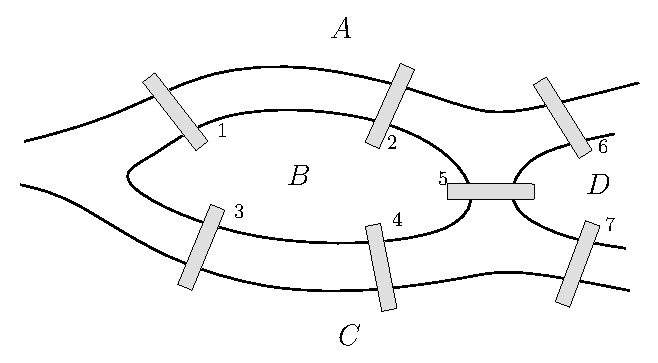
\includegraphics[height=150pt]{eps_imgs/konigsberg}
\caption{Diagrama de la ciudad de K\"onigsberg.}
\label{fig:konigsberg}
\end{figure}

Los habitantes de K\"onigsberg se preguntaban si existía alguna forma de salir de casa, recorrer la ciudad pasando por todos los puentes una vez por cada uno, y regresar a casa.
En la figura~\ref{fig:graph1} se ha hecho una representación simplificada de la ciudad.
Cada punto representa una de las regiones, y cada trazo a un puente.
El problema puede reducirse entonces al de dibujar la figura~\ref{fig:graph1} sin levantar el lápiz y sin repetir ningún trazo, partiendo desde uno de los puntos y volviendo al inicial.

\begin{figure}[h!]
\centering
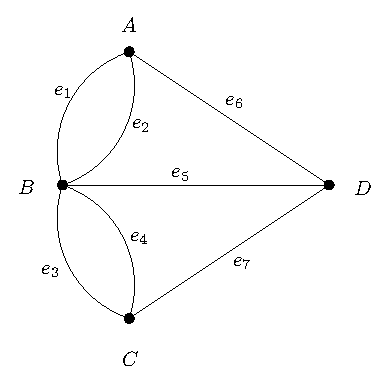
\includegraphics[height=150pt]{eps_imgs/graph1}
\caption{Representación simplificada de la ciudad de K\"onigsberg.}
\label{fig:graph1}
\end{figure}

Con esta reformulación no es difícil argumentar que la respuesta al problema de los puentes es no.
Lo primero es notar que para dibujar la figura~\ref{fig:graph1} debemos para cada punto que no es el incial, ``entrar'' por un trazo y ``salir'' por otro trazo (distinto).
Si notamos en la figura el punto $D$ por ejemplo, tiene tres trazos ``incidiendo'' en él, por lo que después de que se pase por $D$ una vez (se ``entre y salga'' de $D$), la próxima vez que se llegue a $D$ no se podrá salir.
Lo mismo pasa con los puntos $A$ y $C$.
El punto $B$ es un poco diferente, dado que tiene $5$ trazos, se podrá ``entrar y salir'' dos veces, cuando se llegue por tercera vez a $B$ ya no se podrá salir.
El problema entonces surge porque los puntos tienen una cantidad impar de trazos.
Dado que el problema exige que el punto inicial sea igual al punto final, se puede concluir, por la misma razón, que tampoco es posible partir de ninguno de estos puntos ya que el trazo por el que se sale inicialmente de un punto debe ser distinto al con el que se llega finalmente.

El problema entonces tiene que ver con la paridad de los trazos de cada punto.
Basta con que uno de los puntos tenga una cantidad impar de trazos para que la figura no se pueda dibujar siguiendo las reglas pedidas.
Finalmente es imposible recorrer la ciudad completa de K\"onigsberg pasando por todos los punetes y volver a casa.
El primero que dio esta respuesta fue el matemático suizo L. Euler(1707--1783) en el año 1735.
\end{ejemplo}

\begin{ejemplo}
El ejemplo anterior era un poco radical porque todos sus puntos tenían una cantidad impar de trazos.
La figura~\ref{fig:graph2} tampoco se puede dibujar sin repetir trazos y volviendo al punto de partida.

\begin{figure}[h!]
\centering
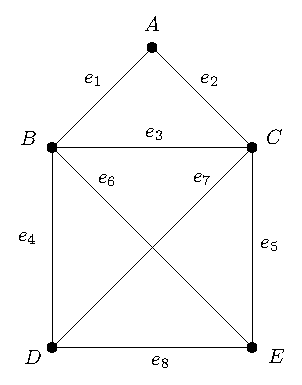
\includegraphics[height=150pt]{eps_imgs/graph2}
\caption{Figura que tampoco se puede dibujar cumpliendo las reglas.}
\label{fig:graph2}
\end{figure}

La razón es la misma que antes, existen puntos con cantidad impar de trazos, en este caso los puntos $D$ y $E$ tienen ambos tres trazos.
Basta con que uno de los puntos de la figura tenga una cantidad impar de trazos para que esta no se pueda dibujar siguiendo las restricciones.
>Qué pasa si una figura tiene todos sus puntos con una cantidad par de trazos?
En este caso nuestra argumentación inicial no sería aplicable si quisiéramos mostrar que no se puede dibujar.
El resultado interesante que veremos más adelante, no dirá que para que una figura se pueda dibujar siguiendo las restricciones, simplemente basta con que todos sus puntos tengan una cantidad par de trazos.
De allí se concluirá que una figura se puede dibujar sin repetir trazos y volviendo al punto de partida, si y sólo si cada punto tiene una cantidad par de trazos.
\end{ejemplo}

Los anteriores ejemplo motivan nuestra definición de grafo.

\begin{definicion}
Un {\bf grafo} $G$ está compuesto por un conjunto de {\bf vértices} que llamaremos $V(G)$, un conjunto de {\bf aristas} que llamaremos $E(G)$, y una relación que a cada arista $e\in E(G)$ le asigna un par de vértices no necesariamente distintos de $V(G)$.

Para representar un grafo se usan puntos para dibujar vértices y trazos para dibujar aristas, cada arista se dibuja como un trazo entre los vértices con los que se encuentra relacionada.
\end{definicion}

\begin{ejemplo}
En ejemplo de la figura~\ref{fig:graph1} el conjunto de vértices es $\{A,B,C,D\}$ y el conjunto de aristas es $\{e_1,e_2,e_3,e_4,e_5,e_6,e_7\}$.
La asignación entre aristas y vértices se puede obtener de la figura, por ejemplo, la arista $e_5$ está relacionada con los vértices $B$ y $D$.

En ejemplo de la figura~\ref{fig:graph2} el conjunto de vértices es $\{A,B,C,D,E\}$ y el conjunto de aristas es $\{e_1,e_2,e_3,e_4,$ $e_5,e_6,e_7,e_8\}$.
La asignación entre aristas y vértices se puede obtener de la figura, por ejemplo, la arista $e_5$ está relacionada con los vértices $C$ y $E$.

Una diferencia importante entre los grafos de las figuras~\ref{fig:graph1} y~\ref{fig:graph2}, es que en el segundo, cada arista está relacionada con un par de vértices distintos.
Nuestra definición de grafo también permite por ejemplo que una arista esté relacionada con un par de vértices iguales.
En la figura~\ref{fig:graph3} se muestra un grafo con aristas de este tipo.
\begin{figure}[h!]
\centering
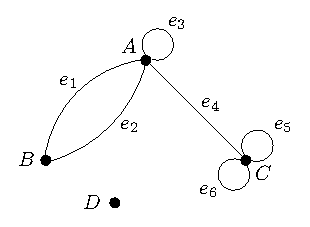
\includegraphics{eps_imgs/graph3}
\caption{Grafo con rulos y aristas paralelas.}
\label{fig:graph3}
\end{figure}
En este grafo el conjunto de vértices es $\{A,B,C,D\}$ y el conjunto de aristas es $\{e_1,e_2,e_3,e_4,e_5,e_6\}$. 
La arista $e_6$ por ejemplo está relacionada con el vértice $C$ (o con el par de vértices $C$ y $C$).
Otra cosa interesante de este grafo es que ninguna arista está relacionada con el vértice $D$, esto para nada escapa de nuestra definición. 
\end{ejemplo}

\begin{definicion}
Un {\bf rulo} en un grafo, es una arista que está relacionada con sólo un vértice.
Dos aristas son {\bf paralelas} si sus pares de vértices relacionados son iguales.

Un grafo de dice {\bf simple} si no tiene rulos ni aristas paralelas.
El grafo de la figura~\ref{fig:graph2} es simple, mientras que los de las figuras~\ref{fig:graph1} y~\ref{fig:graph3} no lo son.

Una arista en un grafo simple puede verse como un par no ordenado de vértices.
Si la arista $e$ está relacionada con los vértices $u$ y $v$, escribiremos $e=uv$ o $e=vu$.
Así podremos decir que un grafo simple es un par $G=(V(G),E(G))$ donde los elementos de $E(G)$ son pares no ordenados de elementos de $V(G)$. 
En el grafo de la figura~\ref{fig:graph2}, podemos decir por ejemplo que $e_4=BD$ y que $e_7=CD$, luego el grafo es $G=(V(G),E(G))$ con $V(G)=\{A,B,C,D,E\}$ y $E(G)=\{AB,AC,BC,BD,CE,BE,CD,DE\}$.
En un grafo simple entonces no es necesario que las aristas tengan nombre, basta identificar al par de vértices que relacionan.
Cuando en un grafo simple $G$ exista una arista $uv\in E(G)$ diremos que $u$ y $v$ son {\bf vecinos} o vértices {\bf adyacentes}, así por ejemplo en el grafo de la figura~\ref{fig:graph2}, $A$ y $B$ son vértices vecinos, al igual que $D$ y $E$.
%
%Dado un grafo $G$, y un vertice cualquiera $v\in V(G)$, se define el {\bf grado} del vértice $v$ como la cantidad de aristas de $G$ que están relacionadas con $v$, cuando el grafo es simple, el grado de $v$ será simplemente la cantidad de vecinos de $v$.
%El grado de $v$ en $G$ lo denotamos por $\delta_G(v)$.
%Cuando el grafo al cual nos refiramos quede claro en el contexto, simplemente escribiremos $\delta(v)$ para referirnos al grado de $v$.

Nosotros estudiaremos principalmente grafos simples.
A menos que se explicite otra cosa, cuando nos refiramos a un grafo nos estaremos refiriendo a un grafo simple con un conjunto no vacío finito de vértices.
\end{definicion}

\subsection{Isomorfismos y Clases de Grafos}

>Cuando dos grafos son estructuralmente equivalentes?
Por ejemplo, >cuál es la diferencia entre los dos grafos de la figura~\ref{fig:compare-graph}?
\begin{figure}[t!]
\centering
\begin{tabular}{cc}
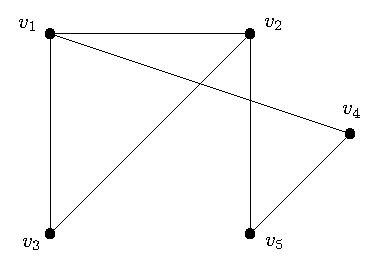
\includegraphics{eps_imgs/graph5}\hspace*{3em} & \hspace*{3em}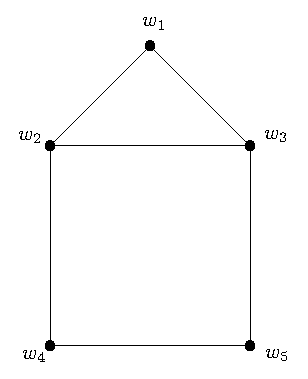
\includegraphics{eps_imgs/graph4} \\
$G_1$ \hspace*{3em} & \hspace*{3em} $G_2$
\end{tabular}
\caption{>Cuál es la diferencia entre $G_1$ y $G_2$?}
\label{fig:compare-graph}
\end{figure}
Ciertamente los dibujos se ven distintos, sin embargo comparten algunas cosas como que ambos tienen la misma cantidad de vértices y la misma cantidad de aristas.
>Pero será que se ven distintos simplemente por la forma en que lo dibujamos?
>Podremos dibujarlos de manera que se ``vean'' iguales?
La respuesta es sí.
En la figura~\ref{fig:transform} se muestra como se pueden ``mover'' los vértices de $G_1$ de manera que se ``vea'' igual a $G_2$.
\begin{figure}[t!]
\centering
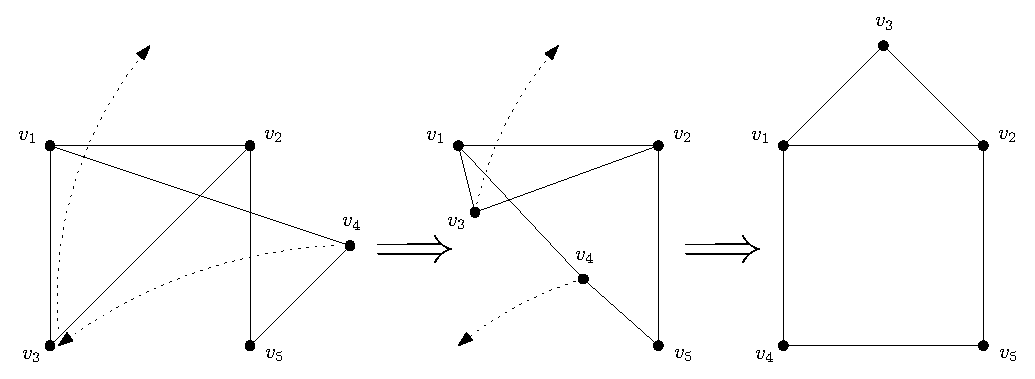
\includegraphics{eps_imgs/graph8}\\
\caption{Transformación de $G_1$.}
\label{fig:transform}
\end{figure}
Lo que estamos haciendo es simplemente ``llevando'' $v_3$ a la posición que ocupa $w_1$ y $v_4$ a la posición que ocupa $w_4$.
Si ahora hacemos un ``renombre'' de los vértices de $G_1$ siguiendo la siguiente regla:
\[
\begin{array}{ccc}
v_1 & \rightarrow & w_2 \\
v_2 & \rightarrow & w_3 \\
v_3 & \rightarrow & w_1 \\
v_4 & \rightarrow & w_4 \\
v_5 & \rightarrow & w_5
\end{array}
\]
obtenemos exactamente a $G_2$.
Esto motiva nuestra definición de equivalencia entre grafos que llamaremos {\bf isomorfismo}.

\begin{definicion}
Dos grafos $G_1$ y $G_2$ se dicen {\bf isomorfos} si existe una función biyectiva $f$ desde $V(G_1)$ a $V(G_2)$, $f:V(G_1)\rightarrow V(G_2)$, tal que $uv\in E(G_1)$ si y sólo si $f(u)f(v)\in E(G_2)$, o sea, si hay una arista entre el par de vértices $u$ y $v$ en $G_1$ si y sólo si hay una arista entre sus imágenes $f(u)$ y $f(v)$ en $G_2$.
Cuando se cumplan estas condiciones, diremos que $f$ es un {\bf isomorfismo} entre $G_1$ y $G_2$.
Escribiremos $G_1\cong G_2$ cuando $G_1$ y $G_2$ sean isomorfos.
No es difícil notar que $\cong$ es una relación de equivalencia entre grafos.
\end{definicion}

\begin{ejemplo}
Los grafos $G_1$ y $G_2$ de la figura~\ref{fig:compare-graph} son isomorfos.
Para demostrarlo basta encontrar una función $f$ biyectiva que cumpla con ser un isomorfismo entre $G_1$ y $G_2$.
La función $f$ es la que ya detallamos:
\[
\begin{array}{ccc}
& f \\
v_1 & \rightarrow & f(v_1)=w_2 \\
v_2 & \rightarrow & f(v_2)=w_3 \\
v_3 & \rightarrow & f(v_3)=w_1 \\
v_4 & \rightarrow & f(v_4)=w_4 \\
v_5 & \rightarrow & f(v_5)=w_5
\end{array}
\]
Primero $f$ es claramente biyectiva.
Ahora debemos comprobar que efectivamente es un isomorfismo, para esto debemos chequear que para cada par de vértices que forman una arista en $G_1$, sus imágenes también forman una arista en $G_2$.
\[
\begin{array}{lclcccccc}
v_1v_2\in E(G_1), & & f(v_1)f(v_2)=w_2w_3 \in E(G_2) \\
v_1v_3\in E(G_1), & & f(v_1)f(v_3)=w_2w_1 \in E(G_2) \\
v_1v_4\in E(G_1), & & f(v_1)f(v_4)=w_2w_4 \in E(G_2) \\
v_2v_3\in E(G_1), & & f(v_2)f(v_3)=w_3w_1 \in E(G_2) \\
v_2v_5\in E(G_1), & & f(v_2)f(v_5)=w_3w_5 \in E(G_2) \\
v_5v_4\in E(G_1), & & f(v_5)f(v_4)=w_5w_4 \in E(G_2) \\
\end{array}
\]
Finalmente $f$ es un isomorfismo de donde concluimos que $G_1\cong G_2$.
\end{ejemplo}
Más adelante veremos técnicas que nos ayudarán a determinar cuándo dos grafos no son isomorfos, por ahora el alumno puede notar que por ejemplo, una condición necesaria (pero no suficiente) para que dos grafos sean isomorfos es que tengan la misma cantidad de vértices y la misma cantidad de aristas.

Otro punto interesante del isomorfismo de grafos y que tiene que ver con computación, es que hasta el día de hoy, nadie ha podido encontrar un algoritmo ``eficiente'' para determinar si dos grafos cualquiera son o no isomorfos.
Volveremos a este punto cuando en el siguiente capítulo definamos la noción de eficiencia de un algoritmo.

La relación $\cong$ es una relación de equivalencia, como tal define clases de equivalencias sobre el conjunto de los grafos.
Estudiaremos algunas de estas clases de equivalencia y les daremos nombre.

\subsection{Algunas Clases de Grafos}

Comenzaremos con un par de definiciones.
\begin{definicion}
Un {\bf camino} es un grafo simple cuyos vértices pueden \emph{ordenarse en una linea} de manera tal que dos vértices son adyacentes si y sólo si son consecutivos en la lista.
Un {\bf ciclo} es un grafo simple cuyos vértices pueden disponerse \emph{en círculo} de manera que dos vértices son adyacentes si y sólo si aparecen en posiciones consecutivas en un círculo.
Un ejemplo de camino y ciclo se muestra en la figura~\ref{fig:graph9}
\begin{figure}[h!]
\centering
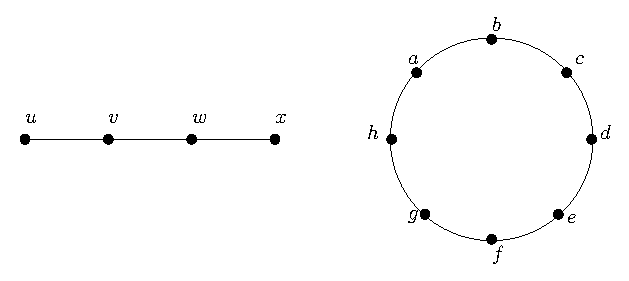
\includegraphics[height=85pt]{eps_imgs/graph9}\\
\caption{Un camino (izquierda) y un ciclo (derecha).}
\label{fig:graph9}
\end{figure}
\end{definicion}

\begin{definicion}
La \emph{clase de equivalencia} de todos los caminos con $n$ vértices la llamaremos $P_n$. 
La \emph{clase de equivalencia} de todos los ciclos con $n$ vértices la llamaremos $C_n$.
En general en vez de hablar de \emph{clase de equivalencia} de grafos, simplemente hablaremos de un grafo particular representante de esta clase, tal que al dibujarlo no nombraremos sus vértices.
Siguiendo esta norma, en la figura~\ref{fig:paths} aparecen $P_4$ y $P_6$.
\begin{figure}[h!]
\centering
\begin{tabular}{cc}
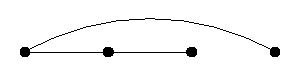
\includegraphics{eps_imgs/p4}\hspace*{3em} &  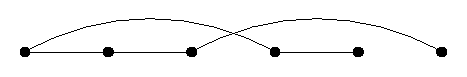
\includegraphics{eps_imgs/p6} \\
$P_4$\hspace*{3em} & $P_6$
\end{tabular}
\caption{Clases de equivalencia para el camino de 4 y 6 vértices.}
\label{fig:paths}
\end{figure}
En ella $P_4$ y $P_6$ se han dibujado a propósito en una disposición no lineal, para enfatizar que lo que importa es su estructura más que el dibujo.
En la figura~\ref{fig:cycle} aparece $C_6$.
\begin{figure}[h!]
\centering
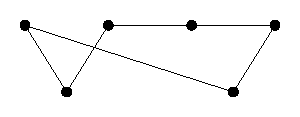
\includegraphics{eps_imgs/c6}\\
$C_6$
\caption{Ejemplo del ciclo con 6 vértices.}
\label{fig:cycle}
\end{figure}
\end{definicion}

Otra clase de grafos importantes es el grafo completo.

\begin{definicion}
Un {\bf grafo completo} es un grafo simple en el que todos los pares de vértices son adyacentes.
Al grafo completo de $n$ vértices le llamaremos $K_n$.
En la figura~\ref{fig:cliques} se pueden ver a los grafos $K_n$ para $n=1,2,3,4,5$.
\begin{figure}[h!]
\centering
\begin{tabular}{ccccc}
	
\includegraphics{eps_imgs/k1} &
	
\includegraphics{eps_imgs/k2} &
	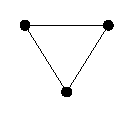
\includegraphics{eps_imgs/k3} &
	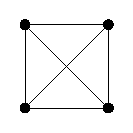
\includegraphics{eps_imgs/k4} &
	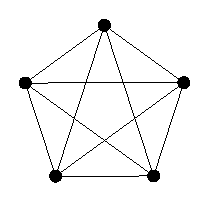
\includegraphics{eps_imgs/k5}\\
	$K_1$ & $K_2$ & $K_3$ & $K_4$ & $K_5$
\end{tabular}
\caption{Grafos completos.}
\label{fig:cliques}
\end{figure}
\end{definicion}

\begin{definicion}
Un grafo $G$ se dice {\bf bipartito} si $V(G)$ se puede agrupar en dos conjuntos disjuntos $V_1$ y $V_2$, $V_1\cap V_2=\emptyset$, $V_1\cup V_2=V(G)$, tal que toda arista en $E(G)$ une a un vértice de $V_1$ con uno de $V_2$.
Esto quiere decir que dos vértices de $V_1$ no pueden ser adyacentes, lo mismo con $V_2$.
\end{definicion}
\begin{figure}[h!]
\centering
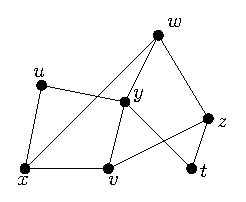
\includegraphics{eps_imgs/graph10}\\
$G$
\caption{Ejemplo de un grafo bipartito}
\label{fig:graph10}
\end{figure}

\begin{ejemplo}
El grafo $G$ de la figura~\ref{fig:graph10} es un grafo bipartito.
El conjunto de vértices de $G$ es $V(G)=\{t,u,v,w,x,y,z\}$, que se puede separar en los conjuntos $V_1=\{t,u,v,w\}$ y $V_2=\{x,y,z\}$ tal que toda arista en $E(G)$ une a un vértice de $V_1$ con uno de $V_2$.
En general, cuando dibujemos un grafo bipartito haremos una clara separación entre las particiones de los vértices ($V_1$ y $V_2$) dibujando los vértices de una de las particiones ``arriba'' de los vértices de la otra partición.
En la figura~\ref{fig:graph11} se ha seguido esta norma para dibujar nuevamente a $G$.
\begin{figure}[h!]
\centering
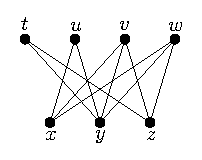
\includegraphics{eps_imgs/graph11}\\
$G$
\caption{El mismo grafo bipartito haciendo una clara diferencia en las particiones.}
\label{fig:graph11}
\end{figure}  
\end{ejemplo}

\begin{ejemplo}
Los grafos bipartitos generalmente se usan para modelar problemas de \emph{asignación} de recursos o tareas.
Podemos suponer que hay vértices de un grafo representando personas y tareas, y que un vértice $p$ correspondiente a una persona es adyacente a un vértice $t$ correspondiente a una tarea si es que la persona $p$ está capacitada para realizar la tarea $t$.
Un grafo de estas características siempre será bipartito.
Un ejemplo se ve en la figura~\ref{fig:job-ass}.
Una pregunta que se puede hacer sobre este tipo de grafos es si existe alguna forma de asignar las tareas de manera tal que toda puedan ser realizadas simultáneamente.
\begin{figure}[h!]
\centering
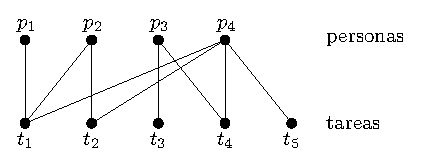
\includegraphics{eps_imgs/graph12}
\caption{Un grafo para modelar un problema de asignación de tareas.}
\label{fig:job-ass}
\end{figure} 
En el grafo de ejemplo esto no es posible (>por qué?).
Más adelante en el curso veremos algunos resultado que nos permitirán establecer cuándo y cuándo no se puede hacer una asignación en grafos de este tipo.
\end{ejemplo}

\begin{definicion}
Un grafo {\bf bipartito completo} es un grafo bipartito en que cada uno de los vértices de una de las particiones es adyacente con cada uno de los vértices de la otra partición.
Cuando las particiones tengan $n$ y $m$ vértices, llamaremos $K_{n,m}$ al grafo bipartito completo.
En la figura~\ref{fig:k2-3} se muestra un diagrama para $K_{2,3}$.
\begin{figure}[h!]
\centering
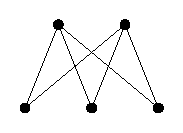
\includegraphics{eps_imgs/k2-3}\\
$K_{2,3}$
\caption{El grafo bipartito completo cuyas particiones tienen tamaño 2 y 3.}
\label{fig:k2-3}
\end{figure}
\end{definicion}
%Terminamos esta subsección con un par de definiciones importantes en la teoría de grafos.

\begin{definicion}
Dado un grafo $G=(V(G),E(G))$, diremos que $H=(V(H),E(H))$ es un {\bf subgrafo} de $G$ si $V(H)\subseteq V(G)$, $E(H)\subseteq E(G)$, y en $E(H)$ aparecen sólo aristas que unen a vértices de $V(H)$.
Cuando $H$ sea subgrafo de $G$, escribiremos $H\subseteq G$.

Un {\bf clique} en un grafo $G$ es un conjunto de vértices $K\subseteq V(G)$ en que para cada par de vértices $u,v\in K$, la arista $uv\in E(G)$.
Un {\bf conjunto independiente} en un grafo $G$ es un conjunto de vértices $K\subseteq V(G)$ tal que para cada par de vértices $u,v\in K$, la arista $uv\notin E(G)$.
El tamaño de un clique o de un conjunto independiente es la cantidad de vértices que lo componen.
\end{definicion}

\begin{ejemplo}
Para el grafo completo $K_n$, se cumple que $\forall i\leq n$, $K_i\subseteq K_n$.
También se cumple que cualquier subconjunto de $V(K_n)$ es un clique en $K_n$.
Los únicos conjuntos independientes en $K_n$ son los conjuntos compuestos por un único vértice de $V(K_n)$.

Para el grafo bipartito completo $K_{n,m}$ con particiones $V_1$ y $V_2$, tanto $V_1$ como $V_2$ son conjuntos independientes.
El clique más grande que se puede encontrar en $K_{n,m}$ está compuesto por dos vértices >por qué?.
Podemos decir también que $C_3$ nunca es subgrafo de $K_{n,m}$,
>puede ocurrir que $C_4\subseteq K_{n,m}$?
>puede ocurrir que $C_5\subseteq K_{n,m}$?
\end{ejemplo}

\begin{definicion}
Dado un grafo $G=(V(G),E(G))$ definimos el {\bf complemento} de $G$ como el grafo $\overline{G}=(V(G),E(\overline{G}))$, en donde el conjunto de arista cumple con $uv\in E(\overline G)\Leftrightarrow uv\notin E(G)$,
o sea $\overline G$ se obtiene a partir de los vértices de $G$ agregando una arista entre cada par de vértices no vecinos en $G$.
Un grafo $G$ se dice {\bf autocomplementario} si ocurre que $G\cong\overline G$.
\end{definicion}

El siguiente teorema nos da una relación entre cliques, conjuntos independientes y el grafo complemento.

\begin{teorema}
\label{teo:clique-indep}
Dado un grafo $G=(V(G),E(G))$ y un subconjunto $V\subseteq V(G)$, entonces $V$ es un clique en $G$ si y sólo si $V$ es un conjunto independiente en $V(\overline G)$.

\begin{demostracion}
Supongamos que $V\subseteq V(G)$ es un clique en $G$, esto quiere decir que para todo $u,v\in V$ ocurre que $uv\in E(G)$.
Por la definición de $\overline G$, sabemos que para todo $u,v\in V$ ocurre que $uv\notin E(\overline G)$ por lo tanto $V$ es un conjunto independiente en $\overline G$.
La implicación inversa se obtiene de manera similar.
\end{demostracion}
\end{teorema}

\begin{ejemplo}
En la figura~\ref{fig:complementos} se muestran tres grafos y sus grafos complemento.
En ella podemos ver que por ejemplo $P_4$ es autocomplementario, que $P_5$ no es autocomplementario, y que el complemento de $K_4$ es un grafo de $4$ vértices \emph{aislados}, ninguno es vecino de otro.
\begin{figure}[h!]
\centering
\begin{tabular}{cc}
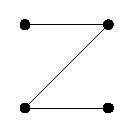
\includegraphics{eps_imgs/p4-2}\hspace*{3em} &  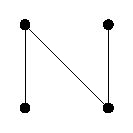
\includegraphics{eps_imgs/p4-2c} \\
$P_4$\hspace*{3em} & $\overline{P_4}$ \\
& \\
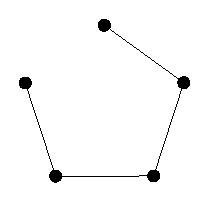
\includegraphics{eps_imgs/p5}\hspace*{3em} &  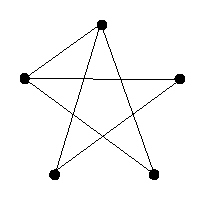
\includegraphics{eps_imgs/p5c} \\
$P_5$\hspace*{3em} & $\overline{P_5}$ \\
& \\
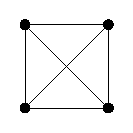
\includegraphics{eps_imgs/k4}\hspace*{3em} &  
\includegraphics{eps_imgs/k4c} \\
$K_4$\hspace*{3em} & $\overline{K_4}$
\end{tabular}
\caption{Algunos grafos y sus complementos}
\label{fig:complementos}
\end{figure}
\end{ejemplo}

\begin{ejemplo}
Dado un conjunto de 6 personas >es cierto que siempre ocurre que hay, o bien tres personas que se conocen mutuamente, o bien tres personas que se desconocen mutuamente?
La respuesta a esta pregunta es SI, y lo justificaremos  modelando el problema con grafos.

Podemos usar un grafo $G$ con 6 vértices $\{p_1,p_2,p_3,p_4,p_5,p_6\}$, cada uno representando a una persona, y agregar la arista $p_ip_j$ si las personas $p_i$ y $p_j$ se conocen.
Queremos demostrar entonces que en cualquier grafo $G$ de 6 vértices ocurre que este o contiene un clique de tamaño 3, o contiene un conjunto independiente de tamaño 3.
Similarmente y usando el teorema~\ref{teo:clique-indep} podemos decir que el problema es equivalente a demostrar que para cualquier grafo de 6 vértices ocurre que, o $G$ tiene un clique de tamaño 3, o $\overline G$ tiene un clique de tamaño 3.
En la figura~\ref{fig:clique-indep} se muestra un posible grafo de $6$ vértices junto a su complemento.
\begin{figure}[h!]
\centering
\begin{tabular}{cc}
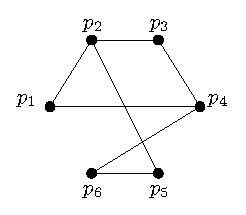
\includegraphics{eps_imgs/graph13}\hspace*{3em} &  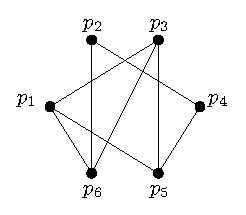
\includegraphics{eps_imgs/graph14} \\
$G$\hspace*{3em} & $\overline G$
\end{tabular}
\caption{Conocidos mutuos y desconocidos mutuos}
\label{fig:clique-indep}
\end{figure}
En el podemos ver que $G$ no tiene un clique de tamaño 3, pero que $\overline G$ si lo tiene, por lo tanto hay tres personas que se desconocen mutuamente (de hecho hay dos de estos grupos, $\{p_1,p_3,p_6\}$ y $\{p_1,p_3,p_5\}$).

Lo que sigue de la demostración la haremos por contradicción suponiendo que ni $G$ ni $\overline G$ tienen un clique de tamaño 3.
La primera observación que haremos es la siguiente:
si miramos una persona en particular, esta o se conoce con al menos tres personas, o se desconoce con al menos tres personas, esto es equivalente a decir que dado un vértice $v$ cualquiera ocurre que, o la cantidad de vecinos de $v$ en $G$ es mayor o igual a 3, o la cantidad de vecinos de $v$ en $\overline G$ es mayor o igual a 3, esto es inmediato del hecho de que todas las aristas que faltan en $G$ aparecen en $\overline G$ (y vice versa).

Enfoquémonos en un vértice en particular $p_i$ y supongamos que su cantidad de vecinos es mayor o igual a 3 en $G$, entonces existen otros tres vértices distintos a $p_i$ y distintos entre sí, $p_j$, $p_k$ y $p_l$ que son vecinos de $p_i$.
Dado que estamos suponiendo que $G$ no tiene un clique de tamaño 3, entonces necesariamente en $G$ $p_j$ no es vecino de $p_k$, $p_j$ no es vecino de $p_l$, y $p_k$ no es vecino de $p_l$, lo que implica que en $\overline G$ los vértices $p_j$, $p_k$ y $p_l$ forman un clique de tamaño tres contradiciendo nuestra suposición de que $\overline G$ no tiene un clique de tamaño 3 (ver figura~\ref{fig:graph15})
Si por el contrario resulta que el vértice particular $p_i$ en el que nos estamos enfocando tiene menos de tres vecinos en $G$, necesariamente este tiene una cantidad de vecinos mayor o igual a 3 en $\overline G$ y podemos usar exactamente el mismo argumento partiendo de $\overline G$ y contradiciendo la suposición de que $G$ no tiene un clique de tamaño 3.
\begin{figure}[h!]
\centering
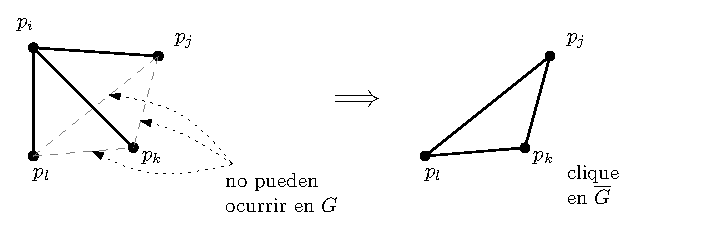
\includegraphics{eps_imgs/graph15}
\caption{Conocidos y desconocidos mutuos.}
\label{fig:graph15}
\end{figure}
\end{ejemplo}

\subsection{Representación Matricial}

Podemos usar una matriz $M_G$ para representar cualquier grafo simple $G$ usando la matriz que representa a la relación \emph{ser vecino de} entre los vértices de $G$, $V(G)$.
Claramente la relación de ser vecino es simétrica por lo que se cumplirá que $M_G=(M_G)^T$, además, dado que $G$ es un grafo simple, la diagonal de $G$ tendrá sólo 0's.
A la matriz $M_G$ se le llama {\bf matriz de adyacencia} de $G$.
Si $G$ tiene $n$ nodos entonces $M_G$ será una matriz de $n\times n$.

\begin{ejemplo}
Para el grafo $G$ de la figura~\ref{fig:clique-indep} la matriz de adyacencia $M_G$ resulta
\[
M_G=
\begin{array}{cc}
& \hspace*{-1.5em}
\begin{array}{ccccccccccc}
p_1\hspace*{-0.5em}& p_2\hspace*{-0.5em} & p_3\hspace*{-0.5em} & p_4\hspace*{-0.5em} & p_5\hspace*{-0.5em} & p_6
\end{array}\\
\begin{array}{c}
p_1\\
p_2\\
p_3\\
p_4\\
p_5\\
p_6
\end{array}
& \hspace*{-1.5em}
\left[
\begin{array}{ccccccccc}
0&1&0&1&0&0 \\
1&0&1&0&1&0 \\
0&1&0&1&0&0 \\
1&0&1&0&0&1 \\
0&1&0&0&0&1 \\
0&0&0&1&1&0 \\
\end{array}
\right]
\end{array}
\]
en donde las filas se han organizado en el orden de los índices de los vértices.
Por su parte la matriz para el grafo $\overline G$ de la misma figura es
\[
M_{\overline G}=
\begin{array}{cc}
& \hspace*{-1.5em}
\begin{array}{ccccccccccc}
p_1\hspace*{-0.5em}& p_2\hspace*{-0.5em} & p_3\hspace*{-0.5em} & p_4\hspace*{-0.5em} & p_5\hspace*{-0.5em} & p_6
\end{array}\\
\begin{array}{c}
p_1\\
p_2\\
p_3\\
p_4\\
p_5\\
p_6
\end{array}
& \hspace*{-1.5em}
\left[
\begin{array}{ccccccccc}
0&0&1&0&1&1 \\
0&0&0&1&0&1 \\
1&0&0&0&1&1 \\
0&1&0&0&1&0 \\
1&0&1&1&0&0 \\
1&1&1&0&0&0 \\
\end{array}
\right]
\end{array}
\]
No es difícil justificar que si $M_G$ es la matriz de adyacencia para $G$, entonces la matriz de adyacencia para $\overline G$ se puede obtener de $M_G$ intercambiando todos los $0$'s por $1$'s excepto en la diagonal.
\end{ejemplo}

La matriz de adyacencia es una forma en que un grafo se le puede entregar a un computador para realizar cierta tarea sobre él.
>Qué pasa cuando $G$ no es un grafo simple?
Supongamos que $G$ es un grafo no necesariamente simple, pero sin rulos, entonces podríamos usar una matriz de adyacencia $M_G$ \emph{extendida} con no solo $0$'s y $1$'s, en que la posición $[M_G]_{(i,j)}=n$ si hay $n$ aristas incidiendo en los vértices que representados por $i$ y $j$.

\begin{ejemplo}
Para el gafo de la figura~\ref{fig:graph16} la matriz de adyacencia \emph{extendida} resulta
\[
\begin{array}{cc}
& \hspace*{-1.2em}
\begin{array}{ccccc}
A&B&C&D\\
\end{array}\\
\begin{array}{c}
A\\
B\\
C\\
D
\end{array}
& \hspace*{-1.2em}
\left[
\begin{array}{ccccc}
0&2&1&1\\
2&0&0&0\\
1&0&0&2\\
1&0&2&0
\end{array}
\right]
\end{array}
\]
en ella las filas se han organizado en el orden alfabético de los vértices.
\end{ejemplo}

Otra forma de representar un grafo matricialmente es usando lo que se llama la {\bf matriz de incidencia}.
En ella las filas se etiquetan con los vértices de $G$ y las columnas con las aristas de $G$.
Si suponemos que $G$ es un grafo no necesariamente simple, pero sin rulos, para cada columna representante de una arista, habrán dos $1$'s uno por cada vértice extremo de la arista.
Si $G$ tiene $n$ vértices y $m$ aristas, entonces su matriz de incidencia será una matriz de $n\times m$.

\begin{ejemplo}
Para el grafo de la figura~\ref{fig:graph16} la matriz de incidencia asociada será
\begin{figure}
\centering
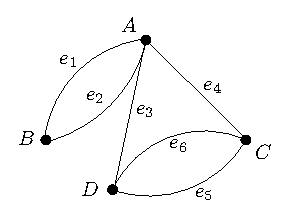
\includegraphics{eps_imgs/graph16}
\caption{Un grafo sin rulos.}
\label{fig:graph16}
\end{figure}
\[
\begin{array}{cc}
& \hspace*{-1.2em}
\begin{array}{ccccccccccc}
e_1\hspace*{-0.5em}&e_2\hspace*{-0.5em}&e_3\hspace*{-0.5em}&e_4\hspace*{-0.5em}&e_5\hspace*{-0.5em}&e_6
\end{array}\\
\begin{array}{c}
A\\
B\\
C\\
D
\end{array}
& \hspace*{-1.2em}
\left[
\begin{array}{ccccccccccccc}
1&1&1&1&0&0\\
1&1&0&0&0&0\\
0&0&0&1&1&1\\
0&0&1&0&1&1
\end{array}
\right]
\end{array}
\]
\end{ejemplo}

Las matrices de adyacencia e incidencia de un grafo $G$ nos sirven para obtener propiedades del grafo y algunas otras propiedades interesantes de conteo. 
Por ejemplo, en un grafo simple si sumamos una fila de la matriz, el resultado es la cantidad de vecinos que tiene el vértice asociado a esa fila.
La siguiente definición tiene que ver con estas propiedades.

\begin{definicion}
El {\bf grado} de un vértice $v$ en un grafo $G$ sin rulos, es la cantidad de aristas de $E(G)$ que están asociadas a $v$.
Cuando $G$ sea un grafo simple el grado de $v$ coincidirá con la cantidad de vecinos.
Al grado del vértice $v$ en el grafo $G$ lo denotaremos por $\delta_G(v)$.
Cuando el grafo que estemos usando quede claro por el contexto, usaremos simplemente $\delta(v)$.
\end{definicion}

La primera implicación interesante para el grado de un vértice tiene que ver con las matrices de adyacencia e incidencia.
Sea $G$ un grafo sin rulos con $n$ vértices y $m$ aristas.
Si al vértice $v_i$ se asocia la fila $i$ de la matriz de adyacencia $M_G$ entonces se cumple que 
\[
\delta_G(v_i)=\sum_{j=1}^{n}[M_G]_{(i,j)}.
\]
Si al vértice $v_i$ se asocia la fila $i$ de la matriz de incidencia $A_G$ entonces se cumple que
\[
\delta_G(v_i)=\sum_{j=1}^{m}[A_G]_{(i,j)}.
\]

Otra propiedad que se puede obtener a partir de la matriz de incidencia tiene que ver con la relación entre los grados de los vértices y la cantidad de arista de un grafo.
Supongamos que tenemos un grafo $G$ sin rulos con $n$ vértices $v_1,v_2,\ldots,v_n$ y $m$ aristas $e_1,e_2,\ldots,e_m$.
Si tomamos la matriz de incidencia de $G$, $A_G$ y sumamos todos los $1$'s que aparecen en ella, esta suma resulta a partir de la doble sumatoria
\begin{equation}\label{eq:incidence-sum}
\sum_{i=1}^{n}\sum_{j=1}^{m}[A_G]_{(i,j)}
\end{equation}
y por el resultado anterior tenemos que
\begin{equation}\label{eq:sum-degree}
\sum_{i=1}^{n}\sum_{j=1}^{m}[A_G]_{(i,j)}=\sum_{i=1}^{n}\delta_G(v_i),
\end{equation}
lo único que hicimos fue reemplazar la sumatoria interna por el grado del vértice correspondiente a la fila que se está sumando.
Ahora si en la expresión~(\ref{eq:incidence-sum}) invertimos el orden de las sumatorias obtenemos
\[
\sum_{j=1}^{m}\sum_{i=1}^{n}[A_G]_{(i,j)}.
\]
Si miramos la nueva sumatoria interna $\sum_{i=1}^{n}[A_G]_{(i,j)}$ su resultado es siempre $2$ para cualquier $j$, esto porque én ella se están sumando los $1$'s que aparecen en una columna determinada de $A_G$, que sabemos que es $2$ porque hay un $1$ por cada vértice extremo de la arista correspondiente a esa columna, con lo que obtenemos
\begin{equation}\label{eq:two-edges}
\sum_{j=1}^{m}\sum_{i=1}^{n}[A_G]_{(i,j)}\sum_{j=1}^{m}2=2m.
\end{equation}
Dado que el orden en que se realizen las sumatorias no altera el resultado, a partir de~(\ref{eq:two-edges}) y~(\ref{eq:sum-degree}) obtenemos la igualdad
\[
\sum_{i=1}^{n}\delta_G(v_i)=2m,
\]
es decir, la suma total de los grados de los vértices es igual al doble de la cantidad de aristas.
Un elegante argumento de conteo del mismo resultado se puede ver en el siguiente diagrama:
\[
\begin{array}{cccc}
& 
\begin{array}{ccccccccccc}
e_1&e_2&e_3&\cdots&e_m
\end{array}
\\
\begin{array}{c}
v_1\\
v_2\\
\vdots\\
v_n
\end{array}
&
\left[
\begin{array}{cccccccccccccccccc}
& & & & & & & & & &  \\
\\
& & & & & A_G\\
\\
\\
\end{array}
\right]
&
\left.
\hspace*{-1em}
\begin{array}{c}
=\delta(v_1)\\
=\delta(v_2)\\
\vdots\\
=\delta(v_n)\\
\end{array}
\right\}
&
\sum_{i=1}^{n}\delta(v_i)
\\
&
\underbrace{
\begin{array}{ccccccccccc}
\shortparallel\hspace*{0.4em}&\shortparallel\hspace*{0.4em}&\shortparallel\hspace*{0.4em}&&\shortparallel\\
2\hspace*{0.4em}&2\hspace*{0.4em}&2\hspace*{0.4em}&\cdots&2
\end{array}
}
&
&
\downarrow
\\
\\
& 
2\times m
&
\rightarrow
&
\sum_{i=1}^{n}\delta(v_i)=2m
\end{array}
\]
$A_G$ es la matriz de incidencia de $G$. 
Para contar todos los $1$'s que aparecen en ella podemos sumar una a una las filas, obteniendo la suma de los grados $\sum_{i=1}^{n}\delta_G(v_i)$, o sumar una a una las columnas obteniendo el doble de la cantidad de aristas, $2\times m$, de donde concluimos que $\sum_{i=1}^{n}\delta_G(v_i)=2m$.

Por la importancia del resultado anterior, lo estableceremos en el siguiente teorema.

\begin{teorema}
Dado un grafo $G$ sin rulos siempre se cumple que 
\[
\sum_{v\in V(G)}\delta_G(v)=2|E(G)|,
\]
o sea, que la sumatoria de los grados de todos los vértices de un grafo, es igual a dos veces la cantidad de aristas del grafo.

\begin{demostracion}
La demostración se sigue de la discusión previa al teorema.
\end{demostracion}
\end{teorema}

Este teorema nos permite establecer un par de corolarios muy importantes.

\begin{corolario}
En un grafo $G$ sin rulos siempre existe una cantidad par de vértices de grado impar.

\begin{demostracion}
La primera observación es que la suma de los grados de todos los vértices de $G$ es par.
%Luego no puede ocurrir que un grafo tenga una cantidad impar de vértice de grado impar ya que, de ser así, el resultado de la suma de todos los grados sería un número impar (sería una suma de una cantidad impar de números impares más cierta cantidad de números pares lo que entregaría un resultado impar).
%
%Un poco más formal.
Ahora, dividamos los vértices de $G$ en dos grupos disjuntos, los que tienen grado par, digamos $u_1,u_2,\ldots,u_p$ y los que tienen grado impar, $w_1,w_2,\ldots,w_q$, o sea, $G$ tiene $p$ vértices de grado par y $q$ vértices de grado impar.
Sean ahora
\[
\begin{array}{rcl}
P &=& \delta(u_1) + \delta(u_2) + \cdots + \delta(u_p) \\
I &=& \delta(w_1) + \delta(w_2) + \cdots + \delta(w_q).
\end{array}
\]
Dado que el resultado de $P+I$ es la suma de los grados de todos los vértices, necesariamente $P+I$ es par.
Ahora, $P$ es claramente par ya que es la suma de sólo números pares por lo que $I$ es par también.
Dado que $I$ es una suma de $q$ números impares, para que $I$ sea par, necesariamente $q$ debe ser un número par, de donde se concluye que $G$ tiene una cantidad par de vértices de grado impar.
\end{demostracion}
\end{corolario}

Los siguientes ejemplo aplican directamente estos resultados.

\begin{ejemplo}
Se quiere organizar un campeonato de fútbol con 25 equipos de manera tal que cada equipo juegue 5 partidos, cada uno contra un equipo distinto. 
>Hay forma de realizar el campeonato?
La respuesta es NO y se obtiene como una consecuencia de los resultados anteriores.

Podemos modelar el problema como un grafo de 25 vértices cada uno representando a un equipo distinto.
El grafo sería tal que hay una arista entre dos vértices si corresponden a dos equipos que jugarán un partido en el campeonato.
Para cumplir la regla de que cada equipo juegue con exactamente $5$ equipos distintos, el grafo debiera ser tal que cada uno de los $25$ vértices tuviese grado $5$, lo que sabemos que no puede ocurrir ya que tendría una cantidad impar de vértices de grado impar.
Por lo tanto el campeonato no puede realizarse siguiendo estas reglas.
\end{ejemplo}
  
\begin{ejemplo}
En el departamento de informática de una empresa trabajan 15 empleados, uno de ellos es la secretaria del departamento y otro es el jefe del departamento, ambos se saludan todos los días y saludan a todos los demás empleados.
Cada uno de los restantes empleados del departamento asegura que diariamente se saluda con exactamente 3 de sus compañeros (sin contar a la secretaria y el jefe) 
>Es esto posible? 

En este caso podemos modelar el problema con un grafo de 15 vértices, uno por empleado, con una arista entre vértices correspondientes a empleados que se saludan.
Dos de los vértices son distinguidos, los correspondientes al jefe y la secretaria, y tienen grado 14 (se saludan con todos).
Los restantes 13 vértices, correspondientes a los demás empleados, debieran tener grado 5 cada uno, ya que se supone que saludan al jefe a la secretaria y a tres de sus compañeros.
Por los resultado anteriores, no puede existir tal grafo ya que tendría una cantidad impar de vértices de grado impar lo que sabemos no puede ocurrir.
\end{ejemplo}


\section{Caminos y Ciclos}

Este tema ya lo motivamos con el ejemplo de los puentes de K\"onigsberg de la sección anterior.
En esta sección nos interesará estudiar algunas propiedades importantes de los grafos que tienen que ver con \emph{caminos} y \emph{ciclos} sobre ellos.
Comenzaremos con un par de definiciones importantes para nuestro siguiente estudio.

\begin{definicion}
Una {\bf caminata} en un grafo (no necesariamente simple) $G$ es una secuencia de vértices y aristas  $(v_0,e_1,v_1,e_2,v_2,\ldots,e_k,v_k)$ tal que para $1\leq i\leq k$, la arista $e_i$ une a los vértices $v_{i-1}$ y $v_i$.
Una {\bf caminata cerrada} en un grafo es una caminata en la que el primer y último vértices son iguales ($v_0=v_k$).
Cuando el grafo es simple, se pueden omitir los nombres de las aristas entre vértices en la representación de una caminata.

Un {\bf camino} en un grafo $G$, es una caminata en la que no se repiten aristas.
Un {\bf ciclo} en un grafo $G$, es una caminata cerrada en la que no se repiten aristas.
(Estas definiciones no debieran causar confusión con las definiciones de $P_n$ y $C_n$ que son clases de grafos, aquí estamos definiendo camino y ciclo \emph{en un grafo dado}, son subgrafos de un grafo dado.)

Una caminata o camino que comience en $u$ y termine en $v$ lo llamaremos caminata $u-v$ o camino $u-v$.
El largo de una caminata, caminata cerrada, camino y ciclo, se obtiene a partir de la cantidad de aristas.
Por simplicidad supondremos que un camino (o ciclo, o caminata) de largo $0$ es un camino (o ciclo o caminata) compuesto por un único vértice sin aristas.
\end{definicion}

\begin{ejemplo}
En el grafo de la figura~\ref{fig:graph16-b} las secuencia:
\begin{figure}[h!]
\centering
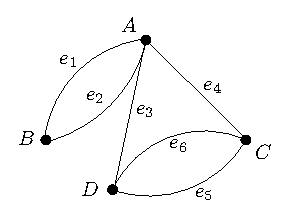
\includegraphics{eps_imgs/graph16}
\caption{Grafo sin rulos}
\label{fig:graph16-b}
\end{figure}
\begin{itemize} 
  \itemsep 0pt
  \item $(D,e_6,C,e_5,D,e_6,C,e_4,A,e_1,B,e_1,A)$ es una caminata pero no un camino, su largo es 6.
  \item $(D,e_6,C,e_5,D,e_6,C,e_4,A,e_1,B,e_1,A)$ es una caminata cerrada pero no un ciclo., su largo es 6.
  \item $(D,e_6,C,e_5,D,e_3,A,e_2,B)$ es un camino, su largo es $4$.
  \item $(D,e_6,C,e_5,D,e_3,A,e_2,B,e_1,A,e_3,D)$ es un ciclo, su largo es $6$.
  \item $(D,e_3,B,e_1,C)$ no es una caminata.
\end{itemize}
En ellos es necesario nombrar las aristas dado que el grafo no es simple.

En el grafo simple de la figura~\ref{fig:graph17} podemos decir que las secuencias:
\begin{figure}[h!]
\centering
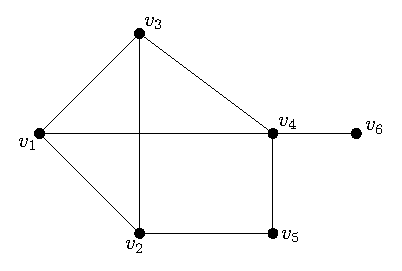
\includegraphics{eps_imgs/graph17}
\caption{Grafo simple}
\label{fig:graph17}
\end{figure}
\begin{itemize}
  \itemsep 0pt
  \item $(v_1,v_4,v_5,v_2,v_3,v_4,v_5)$ es una caminata pero no un camino, su largo es $6$.
  \item $(v_1,v_4,v_5,v_2,v_3,v_4,v_5,v_4,v_1)$ es una caminata cerrada pero no un camino, su largo es $8$.
  \item $(v_1,v_4,v_6)$ es un camino, su largo es $3$.
  \item $(v_1,v_2,v_5,v_4,v_3,v_1)$ es un ciclo, su largo es $5$.
  \item $(v_1,v_5,v_6)$ no es una caminata.
\end{itemize}
En este caso no se nombran las arista ya que quedan implícitas por el hecho de sur un grafo simple.
\end{ejemplo}

\subsection{Conectividad}
\begin{definicion}
Un grafo $G$ se dice {\bf conexo} si para cada par de vértices $u,v\in V(G)$ existe un camino que contiene tanto a $u$ como a $v$.
No es difícil notar que si existe un camino que contiene a un par de vértices $u$ y $v$, entonces existe un camino cuyo vértice inicial es $u$ y final es $v$.
Cuando esto ocurra lo denotaremos por $u\sim v$.
La relación $\sim$, o como la llamaremos ``existe un camino entre'', es una relación de equivalencia sobre los vértices de un grafo.
A un grafo que no sea conexo le llamaremos disconexo.

Dado un grafo $G$, el subgrafo de $G$ compuesto por todos los caminos que contienen un vértice particular se llama {\bf componente conexa} de $G$.
La componente conexa de $G$ a la que pertenece un vértice $v$ particular, contiene a todos los vértices de $G$ que están relacionados con $v$ mediante $\sim$, es decir, todos los vértices de la clase de equivalencia de $v$.
\end{definicion}

\begin{ejemplo}
En la figura~\ref{fig:conex}, $G_1$ es un grafo conexo, mientras que $G_2$ no es conexo, por ejemplo no existe un camino entre los vértices $v_1$ y $v_8$.
En la misma figura, $G_2$ tiene $3$ componentes conexas, $\{v_2,v_6\}$, $\{v_1,v_3,v_5,v_7,v_9\}$, $\{v_4,v_8,v_{10}\}$.
En la figura~\ref{fig:conex-components} se ha dibujado $G_2$ de manera de mostrar claramente sus componentes conexas.
\begin{figure}[h!]
\centering
\begin{tabular}{cccc}
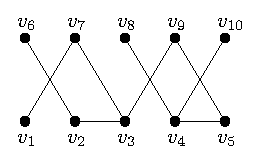
\includegraphics{eps_imgs/graph18} & & & 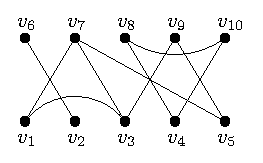
\includegraphics{eps_imgs/graph19} \\
$G_1$ & & & $G_2$
\end{tabular}
\caption{$G_1$ es un grafo conexo, mientras que $G_2$ no lo es.}
\label{fig:conex}
\end{figure}
\begin{figure}[h!]
\centering
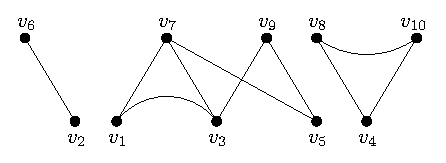
\includegraphics{eps_imgs/graph20}
\caption{Componentes conexas de $G_2$.}
\label{fig:conex-components}
\end{figure}
\end{ejemplo}

>Cuántas aristas puedo agregarle al grafo $G_2$ de la figura~\ref{fig:conex-components} de tal manera que este siga siendo simple y teniendo tres componentes conexas?
>Cuántas aristas puedo sacar de $G$ de manera que este siga teniendo tres componentes conexas?
No es difícil notar que una nueva arisita agregada a un grafo puede disminuir la cantidad de componentes conexas a lo más en $1$, no las modifica si la arista es entre vértices de una misma componente y une dos componentes si la arista es entre vértices de distintas componentes.
De la misma forma, sacar una arista de un grafo puede aumentar la cantidad de componentes conexas a lo más en $1$.
Estas observaciones nos ayudan en el siguiente teorema.

\begin{teorema}\label{teo:min-components}
Un grafo $G$ con $n$ vértices y $k$ aristas tiene al menos $n-k$ componentes conexas.

\begin{demostracion}
Un grafo $G$ con $n$ vértices puede tener como máximo $n$ componentes conexas, cuando no tiene ninguna arista, cada nueva arista que se le agregue puede reducir la cantidad de componentes a lo más en $1$, por lo que luego de agregar $k$ aristas la cantidad de componentes se ha reducido como mínimo a $n-k$, por lo que la cantidad de componentes siempre se mantiene mayor o igual a $n-k$.
\end{demostracion}
\end{teorema}

El anterior teorema implica que si se quiere un grafo conexo de $n$ vértices, entonces al menos $n-1$ aristas son necesarias.
Una definición motivada también por la discusión anterior es la siguiente.

\begin{definicion}
Una {\bf arista de corte} en un grafo $G$ es una arista tal que su eliminación aumenta la cantidad de componentes.
Escribiremos $G-e$ para representar al grafo que resulta de eliminar la arista $e$ a $G$.

Un {\bf vértice de corte} en un grafo $G$ es un vértice tal que su eliminación aumenta la cantidad de componentes. 
Al eliminar un vértice $v$ de un grafo, sacamos $v$ y todas sus aristas incidentes, al grafo resultante lo llamamos $G-v$.
\end{definicion}

\begin{ejemplo}
En el grafo $G_1$ de la figura~\ref{fig:conex}, todas las aristas son de corte, y sus vértices de corte son $v_2,v_3,v_4,v_5,v_7,v_9$.
Un grafo como $G_1$ en el que todas sus aristas son de corte, es un grafo bien particular y lo estudiaremos en la siguiente sección.
En el grafo $G_2$ de la figura~\ref{fig:conex} no hay vértices de corte, y la única arista de corte es $v_2v_6$.
\end{ejemplo}

\begin{ejemplo}
Las aristas y vértices de corte así como la conectividad son conceptos muy importantes a la hora de diseñar una red (o grafo) de comunicación, como una red de computadores que intercambian datos, una red de repetidores de telefonía, o incluso una red de conexiones de vuelo entre ciudades (aquí lo comunicado serían pasajeros entre ciudades).

Tomemos el ejemplo de una red de computadores en la que necesitamos que todos los terminales sean capaces de comunicarse entre sí.
En el grafo asociado a esta red, cada vértice representa a un computador y una arista al cable que conecta un par de computadores.
La primera observación es que este grafo debe ser conexo para que todos los computadores puedan establecer comunicación.
>Que pasa si este grafo tiene algún vértice de corte?
Esto significaría que existe algún computador que, de fallar, haría imposible la comunicación entre algunos de los computadores que no han fallado.
>Qué pasa si este grafo tiene una arista de corte?
Esto significaría que existe alguna conexión (cable) que de fallar haría imposible la comunicación entre alguno de los computadores de la red.
Es interesante que al diseñar una red con un grafo asociado que no tenga ni puntos de corte ni aristas de corte, esta red será automáticamente \emph{tolerante a la falla} de un computador o un cable de comunicación.

En el ejemplo de los vuelos entre ciudades, en el grafo asociado cada vértice representaría a un aeropuerto en alguna ciudad, y una arista representaría la existencia de algún vuelo directo entre un par de aeropuertos.
Si existe un vértice de corte, querría decir que existe un aeropuerto que de ser cerrado dejará a algunas personas sin poder viajar por avión a su destino.
Algo similar pasa con las aristas de corte en este caso.
\end{ejemplo}

Caracterizaremos una arista de corte en términos de ciclos en el grafo.

\begin{teorema}\label{teo:cut-edge}
Una arista en un grafo $G$ es de corte si y sólo si no pertenece a ningún ciclo en $G$.

\begin{demostracion}
Nos centraremos en un grafo $G$ conexo, la demostración se aplicará entonces para cada componente conexa de $G$.

Sea $e=uv$ una arista que pertenece a un ciclo $C$ en $G$, al eliminar $e$ los únicos caminos afectados en $G-e$ son los que contenían a la arista $e=uv$, pero dado que esta pertenece a un ciclo $C$, los caminos afectados pueden completarse con la porción restante de $C$, luego la arista $e$ no puede ser de corte.

Supongamos ahora que $e=uv$ no es una arista de corte, o sea que $G-e$ sigue siendo conexo, esto quiere decir que existe un camino digamos $P$ entre $u$ y $v$ en $G-e$.
El camino $P$ junto con la arista $uv$ forman un ciclo en $G$.

\begin{figure}[h!]
\centering
\hspace*{6em}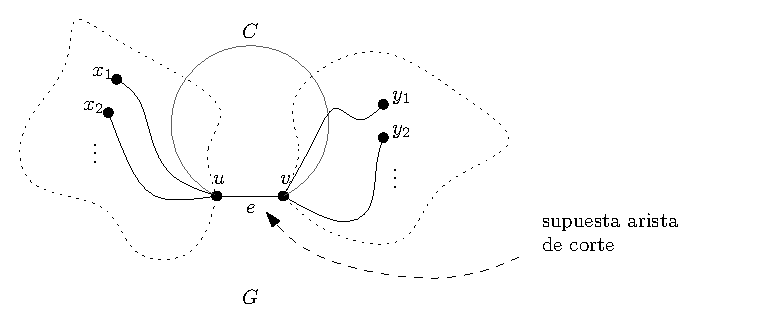
\includegraphics{eps_imgs/cut-edge}
\caption{Una arista es de corte sólo si no pertenece a un ciclo.}
\label{fig:cut-edge}
\end{figure}
La idea central de la demostración se ve en la figura~\ref{fig:cut-edge}, claramente si $e=uv$ pertenece a un ciclo su eliminación no desconectará a $G$.
\end{demostracion}
\end{teorema}

\begin{ejemplo}
En el grafo $G_1$ de la figura~\ref{fig:conex}, ninguna de sus aristas pertenece a un ciclo ya que $G_1$ no tiene ningún ciclo, luego todas sus aristas son de corte.
En el grafo $G_2$ de la misma figura, la única arista que no pertenece a un ciclo es $v_2v_6$ por lo tanto es la única arista de corte.
\end{ejemplo}


\subsection{Grafos Bipartitos}
En esta sección estudiaremos una caracterización de grafos bipartitos en función de ciclos y caminos.

\begin{lema}\label{teo:odd-walk}
En un grafo simple $G$, toda caminata cerrada de largo impar, contiene un ciclo de largo impar.

\begin{demostracion}
Lo haremos usando un argumento inductivo en el largo de la caminata cerrada.
La caminata cerrada más pequeña de largo impar que se puede hacer en un grafo simple es un ciclo de tres vértices, esta caminata ya es un ciclo así que el caso base se comprueba.
Ahora tomemos una caminata $C$ cerrada de largo $l$ impar y supongamos como hipótesis de inducción que toda caminata cerrada de largo impar menor a $l$ tiene un ciclo de largo impar.
Si en $C$ no se repiten vértices entonces $C$ ya es un ciclo de largo impar y comprobamos lo que queríamos, si por otro lado en $C$ se repite un vértice, digamos $v$, entonces podemos partir $C$ en dos caminatas cerradas distintas que comienzan en $v$, $C'$ y $C''$ como se muestra en la figura~\ref{fig:odd-walk}.
\begin{figure}[h!]
\centering
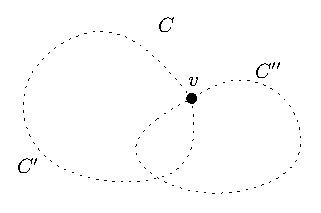
\includegraphics{eps_imgs/odd-walk}
\caption{Una caminata cerrada que repite un vértice, dividida en dos caminatas cerradas}
\label{fig:odd-walk}
\end{figure}
No puede ocurrir que simultáneamente $C'$ y $C''$ tengan largo par ya que entonces $C$ no podría tener largo impar, por lo que al menos una de ellas es una caminata cerrada de largo impar estrictamente menor a $l$ y por HI contiene un ciclo de largo impar, que también será un ciclo de largo impar contenido en $C$ comprobando lo que queríamos.
\end{demostracion}
\end{lema}

El anterior teorema sólo se aplica para caminatas cerradas de largo impar, una caminata cerrada de largo par podría no contener un ciclo de largo par, por ejemplo podría ser una caminata que repitiera todas las aristas dos veces cada una.
El anterior lema nos servirá para demostrar el siguiente teorema.

\begin{teorema}\label{teo:odd-cycle}
Un grafo conexo (simple) $G$  es bipartito si y sólo si no contiene ningún ciclo de largo impar.

\begin{demostracion}
$(\Rightarrow)$ Supongamos que $G$ contiene un ciclo de largo impar, digamos $C=(v_1,v_2,\ldots,v_{k-1},v_k,v_1)$, con $k$ un natural impar, demostraremos que $G$ no puede ser bipartito.
Supongamos que $G$ es bipartito con particiones $V_1$ y $V_2$ y supongamos sin pérdida de generalidad que $v_1\in V_1$.
Dado que $C$ es un ciclo, necesariamente $v_iv_{i+1}\in E(G)$ para $1\leq i< k$ y $v_kv_1\in E(G)$, por lo que debe ocurrir que $v_2\in V_2$, $v_3\in V_1$, $v_4\in V_2$, etc. 
En general debe ocurrir que para los vértices del ciclo $C$, $v_i\in V_1$ si $i$ es impar, y $v_i\in V_2$ si $i$ es par, luego $v_k\in V_1$ lo que es una contradicción con el hecho de suponer que $V_1$ es una partición que contiene a $v_1$ ya que $v_kv_1\in E(G)$.

$(\Leftarrow)$ Supongamos que $G$ no contiene ningún ciclo de largo impar, demostraremos que es posible definir una partición de los vértices de $G$ en dos conjuntos independientes.
Sea $v$ un vértice cualquiera de $V(G)$, definimos $V_1=\{u\in V(G)\;|\;$ existe un camino de largo impar de $v$ a $u\}$, y $V_2=\{u\in V(G)\;|\;$ existe un camino de largo par de $v$ a $u\}$.
Si existiera una arista entre dos vértices de $V_1$ digamos $u_1$ y $u_2$, entonces, dado que existen caminos $v-u_1$ y $v-u_2$ ambos de largo impar, existiría una caminata cerrada de largo impar formada por los dos caminos anteriores más la arista $v_1v_2$ y por el lema~\ref{teo:odd-walk} existiría un ciclo de largo impar contradiciendo nuestra suposición.
Si existiera una arista entre dos vértices de $V_2$ digamos $w_1$ y $w_2$, entonces, dado que existen caminos $v-w_1$ y $v-w_2$ ambos de largo par, existiría una caminata cerrada de largo impar formada por los dos caminos anteriores más la arista $w_1w_2$ y nuevamente por el lema~\ref{teo:odd-walk} existiría un ciclo de largo impar contradiciendo nuestra suposición.
Finalmente no existe arista entre vértices de $V_1$ y no existe aristas entre vértices de $V_2$ y como $G$ es conexo se tiene que $V_1\cup V_2=V(G)$ por lo que $G$ es bipartito con particiones $V_1$ y $V_2$.
\end{demostracion}
\end{teorema}

No es difícil notar que si $G$ no es conexo pero si bipartito, la demostración se aplica a cada componente conexa, y también ocurrirá que $G$ no tendrá ciclos de largo impar.
Para demostrar entonces que un grafo $G$ es bipartito basta dividir los vértices de $G$ en dos conjuntos independientes.
Para demostrar que un grafo $G$ no es bipartito basta encontrar un ciclo de largo impar en $G$.

El alumno podría diseñar un algoritmo para determinar si un grafo es o no bipartito.
El algoritmo debiera ser tal que si el grafo es bipartito entonces el output entregue los conjuntos de vértices que conforman cada partición, y si el grafo no es bipartito el output entregue una secuencia de vértices que formen un ciclo de largo impar en el grafo.

\subsection{Ciclos y Caminos Eulerianos}
En el ejemplo de los puentes de K\"onigsberg los habitantes del pueblo querían encontrar una forma de recorrer la ciudad pasando una vez por cada puente y volviendo al lugar inicial.
Modelamos el problema usando un grafo y dijimos que el problema era equivalente a intentar ``dibujar'' el grafo sin repetir las aristas y volviendo al vértice de donde se inició el dibujo.
Ya argumentamos que si algún vértice del grafo tenía grado impar entonces tal dibujo no se podía lograr.
En esta sección completaremos el resultado, demostrando que esta condición es también suficiente para que un grafo pueda dibujarse siguiendo las restricciones, o sea que un grafo se puede dibujar sin repetir trazos y volviendo al vértice inicial, si y sólo si ninguno de sus vértices tiene grado impar.
Iniciaremos formalizando algunos conceptos.


\begin{definicion}
Un {\bf ciclo Euleriano} en un grafo $G$, es un ciclo que contiene a todas las aristas de $G$ y a todos los vértices de $G$.
Note que es importante que en un ciclo no se repitan aristas, pero perfectamente pueden repetirse vértices.
Diremos que $G$ es un {\bf grafo Euleriano} si contiene un ciclo Euleriano.
\end{definicion}

Según la definición anterior, el problema de los puentes de K\"onigsberg es equivalente a determinar si su grafo asociado es o no Euleriano.
En la figura~\ref{fig:graph21} se muestra un grafo que si es Euleriano, de hecho contiene el siguiente ciclo Euleriano: $(v_1,v_2,v_6,v_7,v_3,v_9,v_{10},v_4,v_8,v_9,v_5,v_7,v_1)$.

\begin{figure}[h!]
\centering
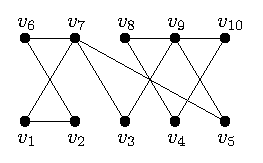
\includegraphics{eps_imgs/graph21}
\caption{Grafo Euleriano.}
\label{fig:graph21}
\end{figure}

Estableceremos ahora el teorema importante de esta sección.

\begin{teorema}\label{teo:euler}
Un grafo $G$ (sin rulos) es Euleriano si y sólo si es conexo y todos sus vértices tienen grado par.

\begin{demostracion}
$(\Rightarrow)$ Supongamos que $G$ es Euleriano, entonces $G$ tiene un ciclo que contiene a todas las aristas y todos los vértices, supongamos que este ciclo parte (y termina) en un vértice particular $v$.
El ciclo necesita una arista para ``salir'' de $v$ y otra para ``llegar'' finalmente a $v$, y cada vez que $v$ aparece nuevamente en el ciclo necesita dos aristas distintas más (una para entrar y otra para salir), un diagrama se ve en la figura~\ref{fig:graph22}.
\begin{figure}[h!]
\centering
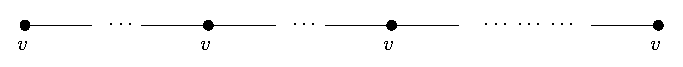
\includegraphics{eps_imgs/graph22}
\caption{Un vértice $v$ particular del ciclo Euleriano y sus artistas incidentes.}
\label{fig:graph22}
\end{figure}
Esto implica que $\delta(v)$ necesariamente es par, ya que todas sus aristas incidentes aparecen en este ciclo una vez cada una.
Este ciclo se puede pensar que parte (y termina) en cada uno de los otros vértices del grafo concluyendo que todos tienen grado par.
Es claro también que si existe tal ciclo, el grafo $G$ es conexo ya que dentro del mismo ciclo se pueden encontrar caminos entre todos los pares de vértices de $G$.

$(\Leftarrow)$ Supongamos que $G$ es conexo y que todos sus vértices tiene grado par.
Demostraremos por inducción en el número de aristas de $G$ que $G$ tiene un ciclo Euleriano.
\begin{inducciondemo}  \BI Para la base de inducción debemos tomar el grafo con el menor número de aristas conexo y con todos sus vértices de grado par.
  Vamos a dividir en dos casos.
  Un primer caso sería un grafo compuesto por un único vértice de grado $0$, claramente este grafo tiene un ciclo Euleriano compuesto por el único vértice del grafo.
	El grafo más pequeño con más de un vértice que cumple las propiedades es el que tiene dos vértices y dos aristas, es claro que este grafo tiene un ciclo Euleriano 
  Con la base de inducción podemos ir un poco más lejos, no es difícil demostrar además que cualquier grafo conexo con $2$ vértices, ambos de grado par siempre contendrá un ciclo Euleriano.
  Todos estos casos base se muestran en la figura~\ref{fig:bi-euler}
 
\begin{figure}[h!]
\centering
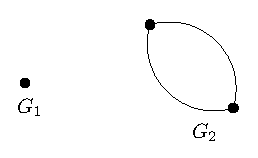
\includegraphics{eps_imgs/bi-euler}
\caption{Los grafos más pequeños conexos y tal que sus vértices tienen grado par.}
\label{fig:bi-euler}
\end{figure}

  \HI Supongamos como hipótesis de inducción que cualquier grafo conexo cuyos vértices tienen grado par y que tiene menos de $n$ aristas tiene un ciclo Euleriano.
  
  \TI Sea $G$ un grafo conexo cuyos vértices tienen grado par y que tiene exactamente $n$ aristas. 
  Dado que ya mostramos en la BI los casos en que $G$ tiene sólo uno o dos vértices, podemos concentrarnos en los casos en que $G$ tiene al menos $3$ vértices distintos.
  Dado que $G$ es conexo y tiene al menos tres vértices, necesariamente debe existir un camino de largo 2 con aristas $e_1$ y $e_2$, que contiene tres vértices, digamos $v_1$, $v_2$ y $v_3$, un diagrama de esto se ve en la figura~\ref{fig:ti-euler1}.
  
  \begin{figure}[h!]
  \centering
  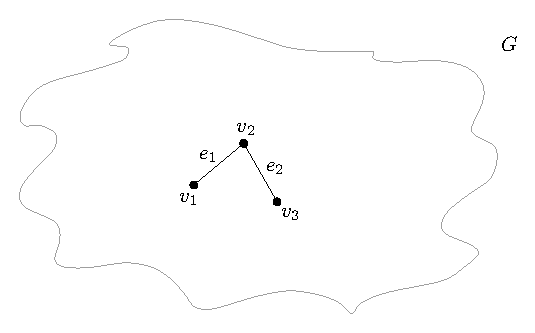
\includegraphics{eps_imgs/ti-euler1}
  \caption{Camino de largo $2$ en un grafo con al menos $3$ vértices.}
  \label{fig:ti-euler1}
  \end{figure}
  
  Podemos crear un nuevo grafo $G'$ a partir de eliminar las aristas $e_1$ y $e_2$ de $G$, y agregar una nueva arista $e$ entre los vértices $v_1$ y $v_3$.
  Un diagrama de $G'$ se ve en la figura~\ref{fig:ti-euler2}.
  \begin{figure}[h!]
  \centering
  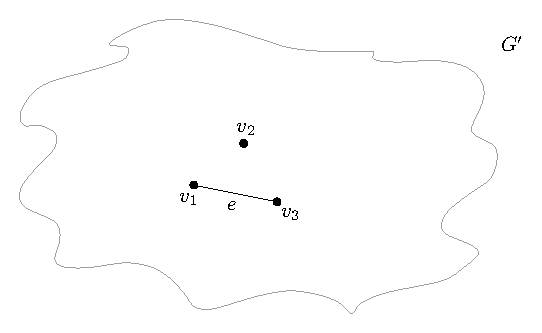
\includegraphics{eps_imgs/ti-euler2}
  \caption{Creación de $G'$ a partir de la eliminación de $e_1$ y $e_2$ y la inserción de $e'$.}
  \label{fig:ti-euler2}
  \end{figure}
  La primera observación es que $G'$ tiene estrictamente menos aristas que $G$.
  Otra cosa que se puede observar es que los únicos vértices que pudieron haber visto afectados sus grado en $G$ son $v_1$, $v_2$ y $v_3$.
  Tanto para $v_1$ y $v_3$ su grado en $G'$ es el mismo que en $G$, para $v_2$ el grado se ha disminuido en $2$, por lo que, dado que en $G$ los tres vértices tenían grado par, en $G'$ también ocurrirá que tienen grado par y por lo tanto $G'$ tiene todos sus vértices de grado par.
  En este punto ``casi'' podemos aplicar la hipótesis de inducción a $G'$, dado que no tenemos seguridad que después del cambio, $G'$ sea un grafo conexo. 
  Nos pondremos entonces en ambos casos, cuando $G'$ resulta ser conexo y cuando no.
  Si $G'$ es conexo entonces cumple con la HI y por lo tanto tiene un ciclo Euleriano digamos $C'$ que contiene a todas las aristas de $G'$ y por lo tanto contiene a $e$, o sea $C'$ es un ciclo Euleriano en $G'$ que contiene la subsecuencia $(v_1,e,v_3)$.
  A partir de $C'$ podemos generar un ciclo para $G$ eliminando la arista $e$ y añadiendo las aristas $e_1$ y $e_2$, o sea cambiando la secuencia $(v_1,e_,v_3)$ de $C'$ por la secuencia $(v_1,e_1,v_2,e_2,v_3)$ este nuevo ciclo es claramente un ciclo que contiene todas las aristas de $G$, por lo tanto $G$ tiene un cilco Euleriano.
  Un diagrama de esta construcción se ve en la figura~\ref{fig:ti-euler3}.
  \begin{figure}[h!]
  \centering
  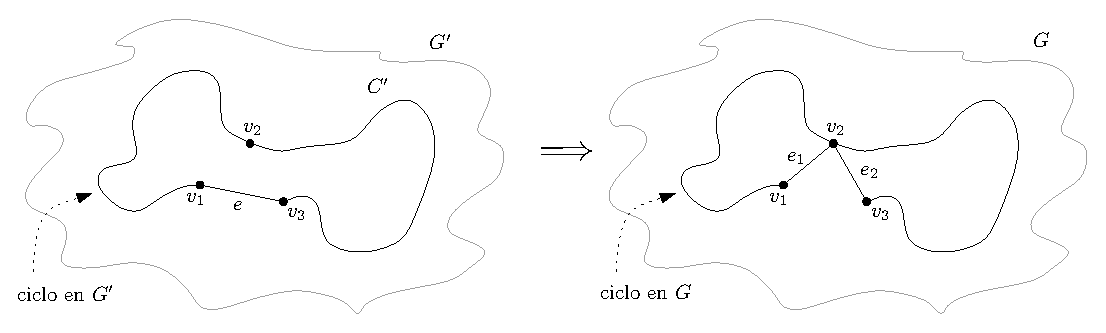
\includegraphics[width=\textwidth]{eps_imgs/ti-euler3}
  \caption{Construcción de un ciclo Euleriano para $G$ a partir de uno para $G'$}
  \label{fig:ti-euler3}
  \end{figure}
  
  Si por otra parte $G'$ no es conexo, dado que $G$ es conexo, $G'$ tendrá dos componentes conexas, una que contendrá a $v_2$, y otra que contendrá a $v_1$ y $v_3$.
  Cada una de estas componentes tendrá sólo vértices de grado par y estrictamente menos aristas que $G$, por lo tanto a cada componente se le aplica la HI.
  Por HI entonces existe un ciclo, digamos $C'$ que podemos suponer que comienza y termina en $v_2$ y contiene a todas las aristas de una de las componentes de $G'$, o sea $C''$ es una secuencia de la forma $(v_2,\ldots,v_2)$.
  Por HI también existe otro ciclo $C''$ que pasa por todas las aristas de la otra componente de $G'$ y que por lo tanto contiene a $e$, o sea $C''$ contiene la subsecuencia $(v_1,e,v,3)$.
  Podría entonces crearse un ciclo para $G$ ``insertando'' $C'$ en $C''$ entre $v_1$ y $v_3$ añadiendo las aristas $e_1$ y $e_2$.
  Un diagrama de esta construcción se ve en la figura~\ref{fig:ti-euler4}.
  
  \begin{figure}[h!]
  \centering
  \includegraphics[width=\textwidth]{eps_imgs/ti-euler4}
  \caption{Construcción de un ciclo Euleriano para $G$ a partir de los ciclos en las dos componentes de $G'$}
  \label{fig:ti-euler4}
  \end{figure}
  
  Por inducción se sigue entonces que cualquier grafo conexo cuyos vértices tiene todos grado par es Euleriano, o sea, contiene un ciclo Euleriano.
\end{inducciondemo}
\end{demostracion}
\end{teorema}

El alumno debiera notar que la demostración además nos entrega un algoritmo para encontrar un ciclo Euleriano en un grafo.
El algoritmo inicialmente realizaría el paso de cambiar un par de aristas por una sola como en la figura~\ref{fig:ti-euler2} y recursivamente debiera encontrar los ciclos del grafo resultante para luego construir un ciclo para el grafo inicial.
Los casos base serían un grafo con un único vértice a con grafo con dos vértices y dos aristas.

\begin{ejemplo}
Supongamos que se tiene un tablero de ajedrez de $n\times n$
>Existe algún valor de $n$ para el cuál el caballo pueda moverse desde un casillero, hacer todas las movidas que son posibles para él en el tablero una vez cada una y volver al casillero inicial?
La respuesta es no, el problema puede modelarse como un grafo, cada casillero representa un vértice y cada movida posible del caballo una arista.
Lo que se quiere entonces es encontrar un ciclo Euleriano.
No es difícil notar que para ningún $n$ (excepto claro $n=1$ existirá un ciclo Euleriano.
Los casos $n=2$ y $n=3$ resultan en grafos no conexos y para $n\leq 4$ el vértice correspondiente a la posición $(1,2)$ del tablero tiene grado $3$, luego existe un vértice de grado impar y por lo tanto no existirá un ciclo Euleriano.
\end{ejemplo}

La siguiente definición relaja un poco la noción de ciclo Euleriano.

\begin{definicion}
Un {\bf camino Euleriano} en un grafo $G$ es un camino no cerrado (el vértice inicial es distinto al final) que contiene a todos los vértices y a todas las aristas de $G$.
Recuerde que para ser un camino, no debe repetir aristas de $G$.
\end{definicion}

\begin{ejemplo}
El grafo de la figura~\ref{fig:graph23} no tiene un ciclo Euleriano ya que por ejemplo el vértice $v_3$ tiene grado 3, pero si tiene un camino Euleriano, de hecho el camino $(v_3,v_2,v_1,v_5,v_2,v_4,v_3,v_5,v_4)$ contiene a todos los vértices y a todas las aristas.
\begin{figure}[h!]
\centering
\includegraphics{eps_imgs/graph23}
\caption{Un grafo que contiene un camino Euleriano.}
\label{fig:graph23}
\end{figure}
\end{ejemplo}

La noción de camino Euleriano captura mucho más nuestra intuición de ``poder dibujar una figura sin levantar el lápiz'', >existirá alguna caracterización para grafos que tengan caminos Eulerianos?
La respuesta es sí y la establecemos en el siguiente teorema.

\begin{teorema}
Un grafo $G$ tiene un camino Euleriano si y sólo si es conexo y contiene exactamente dos vértices de grado impar.

\begin{demostracion}
%Se dará la idea simplemente, los detalles de la demostración se dejan como ejercicio.
$(\Leftarrow)$ Supongamos que en un grafo conexo hay dos vértices de grado impar, digamos $u$ y $v$.
Si al grafo se le agrega una nueva arista para unir $u$ con $v$, el grafo resultante tiene todos sus vértices de grado par por lo que, por el teorema~\ref{teo:euler}, existirá un ciclo Euleriano en él.
Si a este ciclo se le ``borra'' la arista recién agregada resulta un camino que pasa por todos los vértices y aristas del grafo original, o sea un camino Euleriano.

$(\Rightarrow)$ 
Primero si en el grafo existe un camino Euleriano, entonces el grafo es necesariamente conexo (existe un camino entre cada par de vértices).
Supongamos ahora que el camino Euleriano parte en un vértice $v$ y termina en $u$, entonces al agregar una arista nueva $uv$ al camino, se forma un nuevo grafo que contiene un ciclo Euleriano (se cierra el camino).
Por el teorema~\ref{teo:euler} el nuevo grafo necesariamente tiene todos sus vértices de grado par, por lo que en el grafo inicial los únicos vértices de grado impar eran $u$ y $v$, por lo tanto el grafo tiene exactamente dos vértices de grado impar.
\end{demostracion}
\end{teorema}

\subsection{Ciclos Hamiltonianos}

Considere los grafos de la figura~\ref{fig:graph24}
>Es posible encontrar en alguno de ellos, un ciclo que contenga a todos los vértices una véz a cada uno (excepto por el inicial y final)?
Después de probar un poco nos damos cuenta de que en $G_1$ si existe tal ciclo, por ejemplo $(v_1,v_2,v_3,v_4,v_5,v_1)$, pero que en $G_2$ y en $G_3$ es imposible encontrar un ciclo de estas características.
\begin{figure}[h!]
\centering
\includegraphics{eps_imgs/graph24}
\caption{Solo $G_1$ tiene un ciclo Hamiltoniano.}
\label{fig:graph24}
\end{figure}

\begin{definicion}
Un ciclo en un grafo $G$ se dice {\bf ciclo Hamiltoniano} si contiene a todos los vértices de $G$ una única vez a cada uno (excepto por el vértice inicial y final).
A un grafo que contenga un ciclo Hamiltoniano lo llamaremos {\bf grafo Hamiltoniano}.
\end{definicion}

Con esta definición podemos decir que el grafo $G_1$ de la figura~\ref{fig:graph24} es Hamiltoniano, pero que los grafos $G_2$ y $G_3$ de la misma figura no lo son.
Una primera pregunta que podemos hacernos, dada la similitud del problema, es si existe alguna relación entre grafos Eulerianos y grafos Hamiltonianos.
Rápidamente podemos darnos cuenta que no hay una relación directa, por ejemplo, en la figura~\ref{fig:graph24} el grafo $G_1$ es Hamiltoniano pero no Euleriano, $G_2$ no es ni Hamiltoniano ni Euleriano, y $G_3$ es Euleriano pero no Hamiltoniano.

>Existirá alguna propiedad simple de chequear para determinar si un grafo es o no Hamiltoniano?
Hasta el día de hoy nadie ha sido capaz de encontrar una tal propiedad y es bastante poco probable que se encuentre.
Por otra parte nadie ha podido demostrar que no exista una propiedad simple de chequear.
Desde el punto de vista computacional lo anterior nos quiere decir que no existe un procedimiento rápido para determinar si un grafo cualquiera es o no Hamiltoniano, estamos condenados a tener que probar todas las posibilidades para poder responder SI o NO.
La verdad es que si la respuesta es SI, posiblemente no tengamos que probar todas las posibilidades basta con que encontremos un ciclo Hamiltoniano para que nuestra búsqueda acabe, el tema es que si la respuesta es NO, tendremos que asegurarnos de que ninguna posibilidad nos entrega un ciclo Hamiltoniano.
Este es un contraste radical con el de determinar si un grafo es Euleriano, para lo que sabemos que existe un algoritmo muy simple y rápido que responde SI o NO.
El problema de determinar si un grafo tiene o no un ciclo Hamiltoniano es un problema \emph{computacionalmente difícil} y se cree que no puede ser resuelto de manera \emph{eficiente} por un computador.
Más adelante en nuestro estudio nos enfocaremos con más detalle en este tipo de problemas y formalizaremos las nociones de \emph{eficiencia} y \emph{dificultad computacional}.

\begin{ejemplo}
Supongamos que se tiene un tablero de ajedrez de $n\times n$
>Para qué valores de $n$ puede un cabello moverse partiendo de un casillero cualquiera, pasando por todos los otros casilleros una única vez por cada uno y volviendo al casillero inicial?
Nuevamente el problema puede modelarse como un grafo, cada casillero representa un vértice y cada movida posible del caballo una arista. 
El problema se resume a determinar si el grafo resultante es o no Hamiltoniano.
Puede demostrarse que el grafo resultante es Hamiltoniano para todo $n$ par mayor o igual a $6$, sin embargo no hay una propiedad simple de chequear para asgurar esto (como en el caso de un ciclo Euleriano) y la demostración debe ser realizada por separado para cada caso.
\end{ejemplo}


\newpage
\section{Árboles y Grafos en Computación}

Un árbol es una clase especial de grafo y su importancia es tal en las aplicaciones computacionales que lo estudiaremos en una sección por separado.
Junto con el estudio de árboles surge el de problemas de optimización sobre grafos que también tocaremos en esta sección.

\subsection{Árboles}

Supongamos que tenemos una red de computadores como la de la figura~\ref{fig:network} donde los trazos entre computadores representan cables directos entre ellos.
\begin{figure}[h!]
\centering
\includegraphics[width=400pt]{eps_imgs/network}
\caption{Una red de computadores.}
\label{fig:network}
\end{figure}
Esta red cumple con la propiedad de que cualquier computador puede enviar información a cualquier otro en la red (no necesariamente en forma directa), o sea, el grafo asociado a la red es conexo.
Supongamos que quisiéramos construir una red con la propiedad anterior (todos los computadores se puedan comunicar entre ellos) pero minimizando la cantidad de conexiones directas entre computadores.
Un posible resultado se ve en la figura~\ref{fig:tree-network}.
\begin{figure}[h!]
\centering
\includegraphics[width=400pt]{eps_imgs/tree-network}
\caption{Una red de computadores con el mínimo número de conexiones directas.}
\label{fig:tree-network}
\end{figure}
Esta red cumple la misma propiedad anterior, todo computador puede enviar información a cualquier otro computador en la red.
Si nos enfocamos en el grafo asociado a esta nueva red de computadores, una característica crucial que lo diferencia con el anterior es que dado cualquier par de vértices (computadores en la red) existe un único camino que los une.
A un grafo con estas características se le llama {\bf árbol} y su definición se formaliza a continuación.

\begin{definicion}
Un grafo $T=(V(T),E(T))$ es un {\bf árbol} si para cada par de vértices $u,v\in V(T)$ existe un único camino de $u$ a $v$.
Es inmediato de la definición que un árbol es siempre un grafo conexo, dado que para cada par de vértices \emph{existe} un camino (que ``de paso'' es único).
\end{definicion}

\begin{ejemplo}
El grafo correspondiente a la red de la figura~\ref{fig:tree-network} es un árbol.
El grafo de la figura~\ref{fig:graph25} también es un árbol, para comprobarlo basta con notar que entre cualquier par de vértices existe un único camino.
\begin{figure}[h!]
\centering
\includegraphics{eps_imgs/graph25}
\caption{Un árbol.}
\label{fig:graph25}
\end{figure}
\end{ejemplo}

En computación generalmente usamos una clase particular de árboles en los que un vértice particular se distingue de los demás, a este vértice se le llama {\bf raíz} del árbol.

\begin{definicion}
Un {\bf árbol con raíz} (o árbol enraizado, \emph{rooted tree} en inglés) es un árbol $T=(V(T),E(T))$ en que uno de sus vértices $r\in V(T)$ se ha distinguido de los demás. 
Al vértice distinguido $r$ se le llama {\bf raíz} del árbol.
Los vértices en un árbol (con o sin raíz) que tienen grado igual a 1 se llaman {\bf hojas}
(también consideraremos hoja a un vértice de grado 0).
Definiremos más conceptos más adelante.
\end{definicion}
Cuando dibujemos un árbol con raíz, el vértice correspondiente a la raíz se dibujará siempre ``arriba'' y los vértices hoja se dibujarán ``abajo''.
El nombre de árbol se ve motivado por el resultado de dibujar un grafo de estas características, como se puede ver en la figura~\ref{fig:tree}.
\begin{figure}[h!]
\centering
\includegraphics{eps_imgs/tree}
\caption{Árboles (izquierda) en computación y (derecha) en el mundo real... bueno, casi.}
\label{fig:tree}
\end{figure}

Los siguientes teoremas nos entregan caracterizaciones de árboles, formas alternativas de definirlos.

\begin{teorema}
Un grafo $T$ es un árbol si y sólo si $T$ es conexo y no tiene ciclos.\footnote{Aquí nos referimos claramente a ciclos compuestos por más de un único vértice, o sea, a ciclos de largo mayor a 0.}

\begin{demostracion}
$(\Rightarrow)$ Primero si $T$ es un árbol es por definición conexo, nos falta demostrar entonces que un árbol no puede tener ciclos.
Supongamos que $T$ tuviese un ciclo, y sea $C$ un ciclo en $T$ que pasa por los vértices $u$ y $v$.
Supongamos que $C$ parte (y termina) en $u$, entonces $C$ es de la forma $(u,\ldots,v,\ldots,u)$, por lo que se puede dividir en dos porciones, una para ir de $u$ a $v$, digamos $p_1$, y otra (distinta ya que un ciclo no repite aristas) para ir de $v$ a $u$, digamos $p_2$.
Resulta entonces que $p_1$ y $p_2$ son dos caminos distintos entre $u$ y $v$ en $T$, lo que contradice el hecho de que $T$ es un árbol.
La figura~\ref{fig:no-cycle} muestra un diagrama del anterior argumento.
Finalmente $T$ no puede tener ciclos.
\begin{figure}[h!]
\centering
\includegraphics{eps_imgs/no-cycle}
\caption{Formación de dos caminos distintos entre $u$ y $v$ a partir de un ciclo que los contiene.}
\label{fig:no-cycle}
\end{figure}

$(\Leftarrow)$ Como $T$ es conexo, para cada par de vértices existe un camino que los une, falta demostrar que ese camino es único.
Supongamos entonces que $T$ no tiene ciclos pero que sin embargo existe un par de vértices con dos caminos distintos uniéndolos en $T$.
Sea $u$ y $v$ estos vértices y sean $p_1$ y $p_2$ los dos caminos distintos en $T$ que unen a $u$ con $v$.
Dado que estos caminos son distintos entonces ambos tienen al menos tres vértices.
Sea $x$ el vértice anterior al primer vértice que diferencia a $p_1$ y $p_2$ (note que $x_1$ está en $p_1$ y en $p_2$).
Sea $y$ el vértice siguiente a $x$ que pertenece simultáneamente a $p_1$ y $p_2$.
Un diagrama de esto se ve en la figura~\ref{fig:no-two-paths}.
\begin{figure}[h!]
\centering
\includegraphics{eps_imgs/no-two-paths}
\caption{Dos caminos distintos entre el mismo par de vértices siempre contienen un ciclo.}
\label{fig:no-two-paths}
\end{figure}
El camino entre $x$ e $y$ a través de $p_1$ junto con el camino entre $x$ e $y$ a través de $p_2$ forman un ciclo en $T$ lo que contradice nuestra hipótesis de que $T$ no tiene ciclos.
Finalmente no pueden existir dos caminos distintos entre $u$ y $v$, de donde concluimos que para todo par de vértices en $T$ existe un único camino que los une y por lo tanto $T$ es un árbol.
\end{demostracion}
\end{teorema}

\begin{corolario}
Un grafo $T$ es un árbol si y sólo si todas sus aristas son de corte, o sea, para cualquier arista $e$ el grafo $T-e$ no es conexo.

\begin{demostracion}\label{teo:cut-tree}
$(\Rightarrow)$ En la sección anterior (teorema~\ref{teo:cut-edge}) demostramos que una arista es de corte si y sólo si no pertenece a ningún ciclo en el grafo.
Ahora, $T$ es un árbol si y sólo si $T$ es conexo y no tiene ningún ciclo, si y sólo si todas sus aristas cumplen con la propiedad de no pertenecer a un ciclo, si y sólo si, todas sus aristas son de corte.
\end{demostracion}
\end{corolario}

Este corolario debió ser evidente, dado que un árbol tiene el mínimo número de aristas necesarias para que el grafo sea conexo, el sacar cualquier arista desconecta al grafo.
El siguiente corolario no es tan evidente.

\begin{corolario}
Todo árbol es un grafo bipartito.

\begin{demostracion}
En la sección anterior (teorema~\ref{teo:odd-cycle}) demostramos que un grafo es bipartito si y sólo si no contiene ciclos de largo impar.
Si $T$ es un árbol $T$ no contiene ningún ciclo y por lo tanto $T$ es bipartito.
\end{demostracion}
\end{corolario}

La siguiente es una propiedad muy simple de los árboles lo que nos permitirá hacer demostraciones por inducción sobre ellos.

\begin{lema}
Sea $T$ un árbol y $v$ una hoja de $T$, entonces el grafo $T-v$ es también un árbol.

\begin{demostracion}
Para demostrar que el grafo $T-v$ es un árbol debemos comprobar que para cualquier par de vértices en $T-v$, existe un único camino que los une.
Sea $u$ y $w$ dos vértices en $T$ distintos de $v$, y sea la secuencia $P=(u,u_1,u_2,\ldots,u_n,w)$ el único camino en $T$ que une a $u$ con $w$. 
Es claro que el vértice $v$ no aparece en $P$ ya que todos los vértices de $P$ (excepto $u$ y $w$) deben tener grado al menos 2, luego si eliminamos $v$ de $T$ no afecta al camino entre $u$ y $w$, luego el camino $P=(u,u_1,u_2,\ldots,u_n,w)$ entre $u$ y $w$ en $T-v$.
Como la demostración la hicimos en general para un par de vértices cualquiera, en $T-v$ existe un único camino entre todo par de vértices y por lo tanto $T-v$ también es un árbol.
\end{demostracion}
\end{lema}

Con el anterior lema podemos demostrar el siguiente teorema que es una caracterización muy simple de un árbol

\begin{teorema}\label{teo:tree-edges}
Un grafo $T$ con $n$ vértices es un árbol si y sólo si es conexo y tiene exactamente $n-1$ aristas.

\begin{demostracion}
$(\Rightarrow)$ Si $T$ es un árbol con $n$ vértices, entonces claramente es conexo, falta demostrar que tiene exactamente $n-1$ aristas, lo haremos por inducción en $n$.
\begin{inducciondemo}
  \BI Si $n=1$ tenemos un árbol con sólo un vértice y sin aristas, por lo que se cumple la propiedad (la cantidad de aristas es igual a $0 = 1-1 = n-1$).
  \HI Supongamos que un árbol con $n$ vértices tiene exactamente $n-1$ aristas.
  \TI Sea ahora $T$ un árbol con $n+1$ vértices, queremos demostrar que $T$ tiene exactamente $(n+1)-1=n$ aristas.
  Centrémonos en una hoja $v$ cualquiera de este árbol.
  Por el lema anterior $T-v$ también es un árbol y tiene exactamente $n$ vértices por lo que se aplica la HI, luego $T-v$ tiene exactamente $n-1$ aristas.
  Dado que $v$ es una hoja, $v$ tiene grado 1 en $T$ y por lo tanto $T$ tiene exactamente una arista más que $T-v$, o sea $T$ tiene exactamente $n$ aristas, por lo que se cumple la propiedad.
\end{inducciondemo}
Por inducción simple se sigue que todo árbol con $n$ vértices tiene exactamente $n-1$ aristas.

$(\Leftarrow)$ En la sección anterior demostramos  en el teorema~\ref{teo:min-components} que un grafo con $n$ vértices y $k$ aristas tiene al menos $n-k$ componentes conexas.
Si $T$ es un grafo conexo con $n$ vértices y exactamente $n-1$ aristas y tomamos una arista $e$ cualquiera de $T$, entonces dado que $T-e$ tiene $n-2$ aristas, por el teorema~\ref{teo:min-components}, $T-e$ tiene al menos dos componentes conexas y por lo tanto $e$ es una arista de corte.
Dado que elegimos $e$ como una arista cualquiera, $T$ cumple con que todas sus aristas son de corte y por lo tanto (corolario~\ref{teo:cut-tree}) $T$ es un árbol.

\end{demostracion}
\end{teorema}

En nuestro ejemplo inicial nos preguntábamos por la mínima cantidad de conexiones directas necesarias para hacer una red de computadores de manera tal que cualquier computador pudiera enviar información a cualquier otro en la red.
Dado que esto se logra cuando el grafo asociado a la red es un árbol, el teorema anterior nos dice que si tenemos $n$ computadores, la mínima cantidad de estas conexiones será $n-1$.
Este teorema nos da también una forma rápida de chequear si un grafo conexo es o no un árbol, sólo debemos verificar que tenga exactamente una arista menos que vértices.

\subsection{Árboles en Computación}

Ya mencionamos que en computación generalmente usamos árboles con raíz.
Esta noción motiva varias otras definiciones sobre árboles en aplicaciones computacionales.

\begin{definicion}
Sea $T=(V(T),E(T))$ un árbol con raíz $r$, note que, dado que $T$ es un árbol, para cada vértice $x\in V(T)$ existe un único camino de $r$ a $x$.
Definimos lo siguiente:
\begin{itemize}
  \itemsep 0pt
  \item El largo del único camino entre $r$ y un vértice cualquiera $x$ se llama {\bf profundidad} de $x$.
  La raíz $r$ tiene profundidad $0$.
  \item El máximo de las profundidades de todos los vértices de $T$ se llama {\bf altura del árbol} (o {\bf profundidad del árbol}).
  \item La {\bf altura} de un vértice $x$ es la altura del árbol menos la profundidad de $x$.
  \item El conjunto de vértices que aparecen en el único camino de $r$ a $x$ se llaman {\bf ancestros} de $x$.
  Note que $x$ es un ancestro de sí mismo.
  A veces usaremos el término ancestros propios de $x$  para referirnos a los ancestros de $x$ distintos de $x$.
  \item El ancestro propio de $x$ de mayor profundidad se llama {\bf padre} de $x$. 
  Un vértice $x$ es {\bf hijo} de su padre.
  Note que $r$ no tiene padre y que los vértices hoja no tienen hijos.
  \item Si dos vértices $x$ e $y$ tienen el mismo padre diremos que $x$ e $y$ son {\bf hermanos}.
\end{itemize}
La figura~\ref{fig:tree-concepts} muestra gráficamente estas definiciones.

\begin{figure}[h!]
\centering
\includegraphics[height=170pt]{eps_imgs/tree-concepts}
\caption{Definiciones sobre un árbol}
\label{fig:tree-concepts}
\end{figure}
\end{definicion}

Muchas aplicaciones de ordenamiento y búsqueda en computación usan estructuras de datos basadas en un tipo especial de árboles, los llamado árboles binarios.

\begin{definicion}
Un árbol con raíz se dice {\bf árbol binario} si todo vértice tiene a lo más grado 3, o equivalentemente (y cómo se usa más comunmente en computación), si todo vértice tiene a lo más 2 hijos.
En un árbol binario, los hijos de un vértice particular se distinguen en {\bf hijo izquierdo} e {\bf hijo derecho}, lo que también normará las posiciones en las que se dibujen los hijos de cierto vértice.

Note que si a un árbol binario se le elimina una hoja, el grafo que resulta es también un árbol binario (la demostración se deja como ejercicio).
\end{definicion}

Estudiaremos algunas propiedades de los árboles binarios y veremos un caso particular muy útil de este tipo de árboles.

\begin{teorema}
La cantidad de hojas de un árbol binario es uno más la cantidad de vértices con exactamente dos hijo.

\begin{demostracion}
Usaremos la propiedad descrita con anterioridad acerca de que un árbol binario al que se le saca una hoja sigue siendo binario, con esto haremos una demostración por inducción en la cantidad de vértices del árbol binario.
\begin{inducciondemo}
  \BI El caso base es un árbol compuesto por sólo un vértice, la raíz.
  Un árbol de estas características tiene sólo una hoja y ningún vértice con dos hijos, luego cumple la propiedad.
  \HI Supongamos que un árbol binario con $n$ vértices tiene una hoja más que vértices con dos hijos.
  \TI Sea $T$ un árbol binario con $n+1$ vértices, queremos demostrar que $T$ tiene una hoja más que vértices con dos hijos.
  Sea $v$ una hoja cualquiera de $T$, sabemos que $T-v$ es también un árbol binario y tiene exactamente $n$ vértices (uno menos que $T$) por lo que $T-v$ cumple con HI, o sea tiene una hoja más que vértices con dos hijos.
  Supongamos que $T-v$ tiene $k$ vértices con dos hijos entonces por HI tiene $k+1$ hojas >qué podemos decir de $T$?
  Lo que podamos decir dependerá de si $v$ (la hoja que le sacamos) tenía o no un hermano.
  \begin{itemize}
    \item[-] Si $v$ tiene un hermano en $T$, entonces el padre de $v$ es un vértice con dos hijos en $T$.
    Ahora, en el árbol $T-v$, el vértice que era padre de $v$ tiene sólo un hijo.
    Lo anterior quiere decir que $T$ tiene exactamente un vértice más con dos hijos que $T-v$, o sea que $T$ tiene exactamente $k+1$ vértices con dos hijos.
    Ahora también ocurre que $T$ tiene exactamente una hoja más que $T-v$, o sea que $T$ tiene $k+2$ hojas.
    Hemos concluido que $T$ tiene $k+2$ hojas y $k+1$ vértices con dos hijos y por lo tanto cumple con la propiedad.
    \item[-] Si $v$ no tiene hermano, entonces el vértice padre de $v$ en $T$ se convierte en una hoja en el árbol $T-v$, lo que quiere decir que $T$ y $T-v$ tienen exactamente la misma cantidad de hojas, $k+1$.
    El único vértice que ve afectado su cantidad de hijos en $T-v$ es el padre de $v$, este tiene exactamente un hijo en $T$ y $0$ hijos en $T-v$ por lo que la cantidad de vértices con dos hijos en $T$ es también la misma que en $T-v$ e igual a $k$.
    Hemos concluido que $T$ tiene $k+1$ hojas y $k$ vértices con dos hijos y por lo tanto cumple con la propiedad.
  \end{itemize}
  Por inducción en la cantidad de vértices se sigue que todo árbol binario tiene exactamente una hoja más que vértices con dos hijos.
\end{inducciondemo}
\end{demostracion}
\end{teorema}

\begin{ejemplo}
  Un torneo de eliminación simple es un torneo en que cada competencia se realiza entre dos participantes, el participante que pierde la competencia se va del torneo.
  El último participante que permanece en el torneo es el ganador.
  Un ejemplo típico de un torneo de eliminación simple es un campeonato de tenis.
  
  Un torneo de eliminación simple se puede representar por un árbol binario, los participantes iniciales corresponden a las hojas del árbol, el padre de dos vértices corresponde al participante ganador en la competencia realizada entre sus dos hijos, y el participante representado por la raíz del árbol corresponde al ganador del torneo.
   Los ``niveles'' del árbol, o sea las distintas alturas de los vértices, representan las ``rondas'' del torneo, y vértices hojas que no se encuentre a altura $0$ corresponden a participantes que pasan ``libre'' algunas rondas (esto suele ocurrir por ejemplo en los torneos de tenis).
   En la figura~\ref{fig:world-cup-tournament} se ve el resultado de un ``hipotético'' campeonato mundial de futbol desde los cuartos de final, representado por un árbol binario.
   En la figura~\ref{fig:tournament} se ve un torneo más general con participantes que pasan libres ciertas rondas.
   
   \begin{figure}[t!]
   \centering
   \vspace*{200pt}
   %\includegraphics{eps_imgs/world-cup-tournament}
   \caption{Cuartos de final del campeonato mundial de futbol.}
   \label{fig:world-cup-tournament}
   \end{figure}
   \begin{figure}[h!]
   \centering
   \vspace*{200pt}
   %\includegraphics{eps_imgs/tournament}
   \caption{Un torneo de eliminación simple en general con participantes libres en ciertas rondas.}
   \label{fig:tournament}
   \end{figure}
   
   Queremos responder la siguiente pregunta, si tenemos $n$ participantes en un torneo de eliminación simple >cuántos partidos (competencias entre dos participantes) en total se deberán realizar durante el torneo?
   Se podría pensar que esto dependerá de la organización particular del torneo, sin embargo, si nos fijamos que cualquier torneo se puede representar por un árbol binario podremos responder esta pregunta independiente de las decisiones de la organización.
   Ya hemos dicho que cada hoja del árbol asociado corresponde a un participante inicial en el torneo.
   Si un vértice del árbol tiene dos hijos, este corresponde al ganador de un partido entre sus dos vértices hijos, por lo que podríamos asociar un partido con cada vértice que tiene dos hijos en el árbol.
   Finalmente, el teorema anterior nos dice que si el un árbol hay $n$ hojas, entonces la cantidad de vértices con dos hijos es exactamente $n-1$, luego $n-1$ será la cantidad de partidos necesaria realizar durante el campeonato.
   Por ejemplo, $100$ participantes del torneo darán lugar a $99$ partidos en total.
\end{ejemplo}

Una clase especial de árboles binarios nos ayudan para establecer casos límites y cotas para algunos algoritmos de búsqueda, estos son los árboles binarios completos que definiremos a continuación.

\begin{definicion}
  Diremos que $T$ es un {\bf árbol binario completo} si es un árbol binario que cumple con que todos sus vértices que no son hoja tienen exactamente dos hijos y que todas las hojas se encuentran a la misma profundidad.
  
  Si $T$ es un árbol (no necesariamente binario completo) y $v$ es un vértice cualquiera de $T$, el {\bf sub-árbol con raíz en $v$} será el sub-grafo de $T$ compuesto por $v$, todos los vértices que tienen a $x$ como ancestros, y todas las aristas que conectan a estos vértices.
  Es claro que un sub-árbol es también un árbol, que un sub-árbol de un árbol binario es también un árbol binario, y que un sub-árbol de un árbol binario completo es también un árbol binario completo.
\end{definicion}

\begin{teorema}
Un árbol binario completo de altura $H$ tiene exactamente $2^H$ hojas

\begin{demostracion} Por inducción en la altura del árbol
\end{demostracion}
\end{teorema}

\begin{corolario}
Un árbol binario completo de altura $H$ tiene exactamente $2^{H+1}-1$ vértices.

\begin{demostracion}
$2^H$ hojas $\Rightarrow$ $2^{H}-1$ vértices con dos hijos $\rightarrow$ $2^H+2^{H}-1=2^{H+1}-1$ vértices en total.
\end{demostracion}
\end{corolario}

\begin{corolario}
En un árbol binario completo con $n$ vértices su altura es menor o igual que $\log_2(n)$.

\begin{demostracion}
Si la altura es $H$, claramente $n\geq 2^H\Rightarrow \log_2(n)\geq H$.
\end{demostracion}
\end{corolario}

\subsection{Grafos en Computación}
Generalmente en computación nos interesa resolver problemas de optimización sobre grafos para esto el modelo de grafos se extiende un poco.
Las siguientes definiciones introducen el tema.

\begin{definicion}
Un {\bf grafo con peso} es una estructura $G=(V(G),E(G),w)$ donde $V(G)$ es un conjunto de vértices, $E(G)$ es un conjunto de aristas (tal como en un grafo normal) y $w$ es una función de \emph{peso} (o \emph{costo}) $w:E(G)\rightarrow\N$ que a cada arista $e$ de $G$ le asigna un valor que llamaremos peso $w(e)$ (a veces la función puede tener otro conjutno de llegada como $\Z$ o incluso $\R$).
Cuando dibujamos un grafo con peso, generalmente etiquetamos cada arista con su peso correspondiente.

El peso o costo de un camino (caminata, ciclo) en un grafo con peso, es la sumatoria de los pesos de las aristas que componen el camino (caminata, ciclo).
Cuando queremos representar un grafo con peso usando una matriz, usamos una matriz en que cada posición tiene el peso de la arista correspondiente, $0$'s en la diagonal, e $\infty$ si la arista correspondiente no existe (representando que la arista existe pero su peso es demasiado alto como para ser tomada en cuenta).
\end{definicion}

En la figura~\ref{fig:graph26} se muestra un ejemplo de grafo con peso cuya matriz asociada es:
\begin{figure}
\centering
\includegraphics{eps_imgs/graph26}
\caption{Ejemplo de un grafo con peso.}
\label{fig:graph26}
\end{figure}
\[
\left[
\begin{array}{cccccc}
0 & 9 & 6 & 2 & \infty & 3 \\
9 & 0 & 2 & \infty & 3 & 8 \\
6 & 2 & 0 & 4 & 4 & 1 \\
2 & \infty & 4 & 0 & 7 & \infty \\
\infty & 3 & 4 & 7 & 0 & 5 \\
3 & 8 & 1 &\infty & 5 & 0 \\
\end{array}\right]
\]
Sobre un grafo como este se pueden hacer muchas preguntas de optimización como por ejemplo cuál es el camino de menor peso total entre un par de vértices.
En la figura para los vértices $u$ y $v$, la respuesta es $(u,z,w,v)$ de peso total $6$.
El anterior problema suele llamarse el problema del camino más corto.
Cuando estudiamos árboles los introducimos como el grafo con menos aristas que mantiene la propiedad de ser conexo, nos podríamos preguntar en este contexto cuál es el árbol asociado al grafo que tiene menor peso total (siendo el peso total del árbol la suma de los pesos de todas las aristas).
En el grafo de la figura el árbol es el compuesto por las aristas $zw$, $ux$, $vw$, $uz$, $vy$.
El anterior problema suele llamarse el problema del árbol de cobertura de costo mínimo.
Para los dos problemas anteriores existen métodos eficientes que los resuelven, estos métodos suelen estudiarse en detalle en un curso de Algoritmos y Estructuras de Datos.
Otra pregunta que puede hacerse es acerca del ciclo Hamiltoniano de peso total mínimo, sin embargo nuevamente ocurre que para este problema no existe un algoritmo eficiente.

Existen otros tipos de grafos que se usan generalmente para problemas de búsqueda.

\begin{definicion}
Un {\bf grafo dirigido} es una estructura $G=(V(G),E(G))$ muy similar a un grafo normal, pero en que la relación ``ser vecino de'' no necesariamente es simétrica, de echo en un gafo dirigido el conjunto $E(G)$ es un conjunto de pares ordenados de vértices, $E(G)\subseteq V(G)\times V(G)$.

Las definiciones de camino y ciclo se extienden a {\bf camino dirigido} y {\bf ciclo dirigido}.
\end{definicion}

En un grafo normal (no dirigido) estudiamos el problema de la componente conexa.
En un grafo dirigido podemos estudiar un problema similar, cuál conjunto de vértices cumplen la propiedad de que entre cada par de ellos existe un camino dirigido.
Este es el problema de encontrar las componentes {\bf fuertemente conexas} de un grafo.

Se pueden hacer modelos que combinen las dos definiciones anteriores, grafos dirigidos con peso. 
En el se pueden plantear problemas como el de camino dirigido más corto, flujos máximos (suponiendo que el peso de una arista dirigida es la capacidad de un canal), etc.

[...falta completar...]



\newpage
\section{Tópicos Avanzados en Grafos**}

\subsection{Emparejamiento y Cubrimiento}
\subsection{$k$--Conectividad}
\subsection{Planaridad}
\subsection{Grafos Infinitos}



\setcounter{chapter}{2}
\newpage
\thispagestyle{empty}
\chapter{Algoritmos y Problemas Computacionales}
\thispagestyle{empty}

\newpage
\section{Algoritmos}

Formalmente >qué es un algoritmo? no es una pregunta fácil de responder, de hecho, no daremos una definición formal, apelaremos a la intuición que el alumno tenga hasta el momento.
Intuitivamente podemos decir que un algoritmos es un \emph{método} o \emph{conjunto de instrucciones} que sirven para resolver cierto problema.
La duda que puede surgir es >qué clase de problemas pueden ser resueltos por un algoritmo?
Claramente no existe un método para solucionar el problema del hambre en el mundo, o el problema de cómo una persona puede llegar a fin de mes sin deudas.
Diremos entonces que los problemas que nos interesan son los \emph{problemas computacionales}, más adelante definiremos formalmente qué se entiende por problema computacional.
Por ahora nos limitaremos a decir que un problema computacional se plantea en forma de INPUT y OUTPUT: dada una representación de datos de entrada válida INPUT queremos obtener una representación de datos de salida OUTPUT que depende del INPUT y que cumple ciertas condiciones.
Con estos conceptos podemos decir que un algoritmo es un método para convertir un INPUT válido en un OUTPUT.
>Qué significa que un INPUT sea válido? eso dependerá completamente del problema en cuestión.
A este método le exigiremos ciertas propiedades:
\begin{itemize}
  \itemsep 0pt
  \item[-] Precisión: cada instrucción debe ser planteada en forma precisa y no ambigua.
  \item[-] Determinismo: cada instrucción tiene un único comportamiento que depende solamente del input.
  \item[-] Finitud: el método está compuesto por un conjunto finito de instrucciones.
\end{itemize}

Diremos que las instrucciones del algoritmo se \emph{ejecutan}\footnote{Cuando hablemos de la ejecución de las instrucciones de un algoritmo el sujeto siempre será el algoritmo mismo, diremos que él ejecuta las instrucciones.} y que el algoritmo se detiene si no hay más instrucciones que ejecutar o si ya se produjo un OUTPUT.
Un concepto importantísimo es cuándo consideraremos que un algoritmo es correcto.
En nuestro caso diremos que un algoritmo es correcto si para todo INPUT válido luego de comenzar la ejecución del algoritmo, este se detiene y produce un OUTPUT correcto para el INPUT.
Una implicación importante es que de aquí se deduce cuándo un algoritmo es incorrecto: si existe al menos un INPUT válido para el cuál, o el algoritmo no se detiene, o calcula un OUPUT incorrecto, entonces diremos que el algoritmo es incorrecto.

El alumno debe estar acostumbrado a los ejemplos tipo ``receta de cocina'' muy comentados en cursos introductorios de computación.
Nos evitaremos este tipo de ejemplos e introduciremos nuestra notación de algoritmo con un problema más cercano a lo que nos interesará en este curso.
Para representar un algoritmo usaremos seudo--código, muy parecido a lo que sería un código en un lenguaje como C o Java pero que no se preocupa de problemas de sintaxis y en algunos casos nos permitirá trabajar de manera simple con conjuntos, operaciones matemáticas, etc.

\begin{ejemplo}
Queremos un algoritmo para, dada una secuencia $S=(s_1,s_2,\ldots,s_n)$ de $n$ números enteros de input, genere como output el valor máximo de esa secuencia.
El siguiente es un algoritmo ``iterativo'' que resuelve el problema planteado:
\begin{codebox}
\Procname{INPUT: Una secuencia $S=(s_1,s_2,\ldots,s_n)$ y un natural $n\geq 1$ que representa el largo de la secuencia. \\
OUTPUT: $m=\max\{s_1,s_2,\ldots,s_n\}$, el máximo de los números de la secuencia.

$\proc{Max}(S,n)$}
\li $m\cgets s_1$
\li $k\cgets 2$
\li \While $k\leq n$ \Do
\li \> \If $s_k > m$ \Then
\li \> \> $m\cgets s_k$
\li \> $k\cgets k+1$
\li \Return $m$
\end{codebox}

El siguiente es un algoritmo ``recursivo'' que resuelve el problema planteado:
\begin{codebox}
\Procname{INPUT: Una secuencia $S=(s_1,s_2,\ldots,s_n)$ un natural $n\geq 1$ que representa el largo de la secuencia. \\
OUTPUT: $m=\max\{s_1,s_2,\ldots,s_n\}$, el máximo de los números de la secuencia.

$\proc{Rec-Max}(S,n)$}
\li \If $n=1$ \Then
\li \> \Return $s_1$
\li \Else
\li \> $k:=\proc{Rec-Max}(S,n-1)$
\li \> \If $s_n\geq	k$ \Then
\li \> \> \Return $s_n$
\li \> \Else
\li \> \> \Return $k$
\end{codebox}
\end{ejemplo}

En el ejemplo se han introducido algunas instrucciones que debieran resultar familiares, {\bf while}, {\bf if}--{\bf else}, {\bf return}, que tienen el sentido habitual de un lenguaje de programación de propósito general, hemos usado el operador ``$:=$'' para la asignación, y a veces usaremos también la instrucción {\bf for}.
También se ha introducido la forma de hacer recursión.
Los algoritmos recursivos en general tienen relación directa con definiciones inductivas de objetos (como vimos en la sección 1.1).
Supondremos que el alumno tiene cierta familiaridad también con algoritmos recursivos.
En el algoritmo recursivo anterior se está aprovechando la definición inductiva del máximo de una secuencia de elementos:
\begin{enumerate}
  \itemsep 0pt
  \item $\max\{s_1,s_2,\ldots,s_n\}=\max\{\max\{s_1,s_2,\ldots,s_{n-1}\},s_n\}$
  \item $\max\{s_1\}=s_1$.
\end{enumerate}
En general los algoritmos recursivos se obtendrán casi en forma directa de definiciones inductivas de objetos o propiedades.
 
>Cómo podemos asegurar que los anteriores algoritmos son correctos, o sea, que siempre se detienen y entregan el resultado esperado?
La forma en cómo se diseñaron nos da una intuición de su \emph{corrección}, pero necesitamos métodos más formales para establecer la corrección de un algoritmo.


\subsection{Corrección de Algoritmos}
La herramienta principal que usaremos para demostrar la corrección de los algoritmos será la inducción en sus distintas formulaciones.
Dividiremos nuestro estudio en dos partes, la corrección de algoritmos iterativos y la corrección de algoritmos recursivos.

\subsubsection*{Corrección de Algoritmos Iterativos}
Supongamos que queremos demostrar que un algoritmo no recursivo (o sea, uno en que no hay llamadas recursivas a sí mismo) es correcto. 
La única dificultad proviene de la posibilidad de que el programa contenga \emph{loops}, o sea que realice iteraciones, por lo que nos centramos en este caso\footnote{No nos preocuparán algoritmos no recursivos que no tengan iteraciones ya que en ellos se puede hacer un trazado completo de su ejecución viendo todos los casos y la corrección resulta trivial}.
Generalmente, dividimos la demostración de que un programa iterativo es correcto en dos tareas independientes, que llamamos {\bf corrección parcial} y {\bf terminación} que se definen de la siguiente forma.
Para demostrar la corrección parcial de un algoritmo debemos establecer que, si el algoritmo se detiene, entonces entrega un resultado correcto.
Para la terminación debemos demostrar que el algoritmo efectivamente se detiene.
Introduciremos estos conceptos con un ejemplo.

El siguiente es un algoritmo que recibe como input un par de números naturales $x$ e $y$, analizaremos luego cuál es el output del algoritmo.
\begin{codebox}
\Procname{INPUT: Dos números $x,y\in\N$. \\
OUTPUT: $z=$ ?.

$\proc{M}(x,y)$}
\li $z:=0$
\li $w:=y$
\li \While $w \not= 0$ \Do
\li \> $z:=z+x$
\li \> $w:=w-1$
\li \Return $z$
\end{codebox}

En este algoritmo existe un único \emph{loop}.
Para demostrar la corrección parcial de un algoritmo, lo que generalmente se hace es buscar un {\bf invariante} del \emph{loop}, una expresión lógica que sea verdadera antes de iniciar el \emph{loop} y al final de cada una de las iteraciones del \emph{loop}.
Esta expresión siempre tendrá relación con las variables del algoritmo y generalmente es una expresión que ``une a las variables'', las hace depender unas de otras.
Si encontramos una expresión y logramos demostrar que esta es efectivamente un invariante, entonces esta expresión será verdadera también al finalizar el \emph{loop}, luego de su última iteración, lo que nos permitirá decir que, si el \emph{loop} se detiene entonces la propiedad se cumple.
Dado un \emph{loop} pueden existir muchas propiedades que siempre sean verdaderas antes de iniciar y al final de cada iteración, debemos elegir la que más información nos entregue con respecto a lo que el algoritmo pretende realizar.
Por ejemplo, en el anterior algoritmo está claro que la expresión:
\[
0\leq w\leq y
\]
es un invariante del loop, el problema principal es que no nos dice nada por ejemplo de los valores de las variables $x$ y $z$ que también están participando del algoritmo.

>Cómo buscamos entonces un invariante que nos ayude a demostrar la corrección parcial?
En general debemos centrarnos en buscar propiedades que tengan que ver con lo que queremos que el algoritmo haga.
>Qué hace el anterior algoritmo?
No es difícil notar que el algoritmo anterior, en base a sumas y decrementos, calcula la multiplicación entre $x$ e $y$, por lo que al finalizar el algoritmo se debiera cumplir que $z=x\cdot y$.
Para estar más seguros podemos hacer una tabla con los valores que toman cada variable después de cada iteración.
La siguiente es la tabla mencionada si se supone que los valores de $x$ e $y$ son inicialmente $a$ y $b$, la columna $0$ corresponde a los valores antes de que comience el \emph{loop} y la columna $i$ a los valores al finalizar la $i$--ésima iteración.
\[
\begin{array}{c|ccccccc}
\text{variables} & 0 & 1 & 2 & 3 & 4 & \ldots & b \\ \hline
x & a & a & a &     a  & a  & \cdots & a \\
y & b & b & b &     b  & b  & \cdots & b \\
z & 0 & a & 2a &    3a & 4a & \cdots & b\cdot a \\
w & b & b-1 & b-2 & b-3& b-4& \cdots & 0
\end{array}
\]
El \emph{loop} alcanza a ejecutar $b$ iteraciones luego de lo cuál el valor de $w$ se hace $0$ y se termina con $z=b\cdot a$ que era lo que esperábamos.
Esta tabla nos permite inferir también que la siguiente expresión debiera cierta luego de cada iteración del \emph{loop}:
\[
z=(y-w)x
\]
Si demostráramos que la expresión anterior es un invariante entonces estaríamos seguros que después de la última iteración del \emph{loop} se cumple que $z=(y-w)x$, y dado que el \emph{loop} se detiene sólo si $w=0$ obtendríamos que, si el algoritmo se detiene entonces $z=y\cdot x$.
Para demostrar que $z=(y-w)x$ es un invariante usaremos el principio de inducción simple, en el siguiente lema.

\begin{lema}
La expresión $z=(y-w)x$ es un invariante para el loop del algoritmo $\proc{M}(x,y)$, o sea,
si $x,y\in\N$ y se ejecuta el algoritmo $\proc{M}(x,y)$ entonces luego de cada iteración se cumple que $z=(y-w)x$.

\begin{demostracion}
Las únicas variables que cambian sus valores a medida que el algoritmo se ejecutan son $z$ y $w$, luego hay que centrarse en la evolución de los valores de estas variables.
Sean $z_i$ y $w_i$ los valores que almacenan las variables $z$ y $w$ luego de que se termina la $i$--ésima iteración del algoritmo, $z_0$ y $w_0$ son los valores iniciales.
Demostraremos por inducción que para todo $i$ se cumple que $z_i=(y-w_i)x$.
\begin{inducciondemo}
  \BI Para $i=0$, se tiene que $z_i=z_0=0$ y que $w_i=w_0=y$.
  Ahora, $z_0=0=(y-y)x=(y-w_0)x$ por lo que se cumple que $z_i=(y-w_i)x$ para $i=0$.
  \HI Supongamos que efectivamente se cumple que $z_i=(y-w_i)x$.
  \TI Al final de la iteración $i+1$ el valor de $z$ se ha incrementado en $x$ y el valor de $w$ se ha decrementado en $1$ por lo que se cumple la relación $z_{i+1}=z_i+x$ y $w_{i+1}=w_i-1$.
  Ahora
  \[
  z_{i+1}=z_i+x\stackrel{HI}{=}(y-w_i)x+x=(y-w_i+1)x=(y-(w_i-1))x=(y-w_{i+1})x
  \]
  por lo que la propiedad también se cumple para $i+1$.
\end{inducciondemo}
Por inducción entonces se ha demostrado que después de cada iteración se cumple que $z=(y-w)x$ y por lo tanto si el algoritmo termina, el resultado será $z=y\cdot x$
\end{demostracion}
\end{lema}

Hemos demostrado la corrección parcial del algoritmo, ahora debemos demostrar que el algoritmo efectivamente termina, generalmente esta parte es más simple de demostrar, y casi siempre basta con encontrar una expresión entera que decrezca o se incremente con cada iteración y argumentar que llegado a cierto valor en la sucesión el algoritmo se detendrá
El siguiente lema demuestra la terminación del anterior algoritmo.

\begin{lema}
Si $x,y\in\N$ y se ejecuta el algoritmo $M(x,y)$ entonces este se detiene.

\begin{demostracion}
Note que el valor de $w$ es inicialmente $y\in\N$ y después de cada iteración se decrementa en $1$.
Los valores de $w$ forman entonces una sucesión siempre decreciente de valores consecutivos que se inicia en un número natural, por lo que en algún momento $w$ tomará el valor $0$ (ya que $0$ es el menor de los números naturales) y por lo tanto el \emph{loop} terminará y también el algoritmo.
\end{demostracion}
\end{lema}

Finalmente con los dos lemas anteriores se demuestra directamente el siguiente teorema.

\begin{teorema}
El algoritmo $M(x,y)$ retorna el valor $x\cdot y$ (cuando $x,y\in\N$).

\begin{demostracion}
Directa de los dos lemas anteriores.
\end{demostracion}
\end{teorema}

Podemos usar esta misma estrategia para demostrar que el algoritmo iterativo $\proc{Max}(S,n)$ es también correcto, o sea, que después de ejecutarlo con una secuencia $S$ de valores y un natural $n\in\N$ correspondiente a la cantidad de valores de la secuencia, el algoritmo retorna el máximo de la secuencia $S$.
En el siguiente ejemplo se discuten algunos aspectos de esta demostración.

\begin{ejemplo}
Demostraremos que si el algoritmo $\proc{Max}(S,n)$ del principio de esta sección se ejecuta con una secuencia $S$ de $n$ valores $s_1,s_2,\ldots,s_n$ entonces retorna el máximo de la secuencia.
Nos evitaremos la formalidad de establecer teoremas y lemas para la demostración.

Lo primero es notar que el algoritmo termina, su justificación se deja como ejercicio.
Ahora debemos justificar que si el algoritmo termina calcula el resultado correcto.
Debemos encontrar un invariante del \emph{loop} del algoritmo, una expresión que siempre se mantenga verdadera.
Dado que las únicas variables que se modifican durante la ejecución son $m$ y $k$ debemos encontrar una invariante que incluya a estas dos variables y a los valores de la secuencia $S$.
Proponemos el siguiente invariante: en todo momento se cumple que
\begin{equation} \label{eq:inv-max}
m\in S\text{ y }m\geq s_1,s_2,\ldots,s_{k-1}
\end{equation}
o sea, en todo momento $m$ es mayor o igual a los $k-1$ elementos iniciales de $S$.
Nótese que si demostramos que~(\ref{eq:inv-max}) es efectivamente un invariante entonces, dado que al terminar el algoritmo el valor de $k$ es $n+1$, sabríamos que al terminar el algoritmo $m$ es efectivamente el máximo.
La primera parte del invariante ($m\in S$) es simple de justificar ya que basta mirar el código para notar que cada asignación posible a $m$ es con uno de los valores $s_i$.
La que es un poco más complicada es la segunda parte que la demostraremos por inducción.
Sean $m_i$ y $k_i$ los valores de las variables $m$ y $k$ al finalizar la $i$--ésima iteración del \emph{loop}, por inducción demostraremos que para todo $i$ se cumple que 
\[
m_i\geq s_1,s_2,\ldots,s_{k_i-1}
\]
\begin{inducciondemo}
  \BI Para $i=0$ (o sea antes de comenzar la primera iteración del \emph{loop}) se cumple que $m_i=m_0=s_1$ y que $k_i=k_0=2$, por lo que $m_i=s_1\geq s_1=s_{2-1}=s_{k_i-1}$.
  \HI Supongamos que al final de la iteración $i$ efectivamente se cumple que $m_i\geq s_1,s_2,\ldots,s_{k_i-1}$.
  \TI Al final de la iteración $i+1$ el valor de $k$ se incrementa en $1$ por lo que $k_{i+1}=k_i+1$.
  Ahora el valor de $m$ se modifica dependiendo del resultado del {\bf if} de las líneas 4--5, dependiendo de su comparación con el valor $s_k$.
  Algo muy importante de notar es que al momento de la comparación en el {\bf if}, los valores de $m$ y $k$ que se comparan son los correspondientes a la iteración anterior ($i$ en nuestro caso).
  Tendremos entonces dos casos dependiendo del resultado del {\bf if}: (1) $m_{i+1}=m_i$ si $m_i\geq s_{k_i}$, o (2) $m_{i+1}=s_{k_i}$ si $s_{k_i}>m_{i}$.
  Dividiremos entonces la demostración:
  \begin{itemize}
    \item[(1)] Si $m_i\geq s_{k_i}$, entonces al final de la iteración $i+1$ sabemos que $m_{i+1}=m_i$ y $k_{i+1}=k_i+1$.
    Por HI sabemos que $m_i\geq s_1,s_2,\ldots,s_{k_i-1}$ y como además sabemos que $m_i\geq s_{k_i}$ podemos concluir que $m_i\geq s_1,s_2,\ldots,s_{k_i-1},s_{k_i}$.
    Ahora, dado que en este caso $m_{i+1}=m_i$ obtenemos que
    \[
    m_{i+1}=m_i\geq s_1,s_2,\ldots,s_{k_i-1},s_{k_i}.
    \] 
    Cómo también sabemos que $k_{i+1}=k_i+1$, se cumple que $s_{k_i}=s_{k_{i+1}-1}$, así finalmente obtenemos que
    \[
    m_{i+1}\geq s_1,s_2,\ldots,s_{k_{i+1}-1}
    \] 
    que es lo que queríamos demostrar.
    \item[(2)] Si $s_{k_i}>m_i$, entonces al final de la iteración $i+1$ sabemos que $m_{i+1}=s_{k_i}$ y $k_{i+1}=k_i+1$.
    Por HI sabemos que $m_i\geq s_1,s_2,\ldots,s_{k_i-1}$ y como además sabemos que $s_{k_i}>m_i$  
    obtenemos que $s_{k_i}\geq s_1,s_2,\ldots,s_{k_i-1}$.
    Ahora, dado que en este caso $m_{i+1}=s_{k_i}$ y es claro que $s_{k_i}\geq s_{k_i}$ obtenemos que
    \[
    m_{i+1}=s_{k_i}\geq s_1,s_2,\ldots,s_{k_i-1},s_{k_i}.
    \]
    Cómo también sabemos que $k_{i+1}=k_i+1$, se cumple que $s_{k_i}=s_{k_{i+1}-1}$, así finalmente obtenemos que
    \[
    m_{i+1}\geq s_1,s_2,\ldots,s_{k_{i+1}-1}
    \] 
    que es lo que queríamos demostrar.
  \end{itemize}
  Finalmente la propiedad también se cumple para $i+1$.
\end{inducciondemo}
Por inducción hemos demostrado que~(\ref{eq:inv-max}) es efectivamente un invariante para el algoritmo $\proc{Max}(S,n)$ y que por lo tanto siempre se cumple que $m\in S$ y $m\geq s_1,s_2,\ldots,s_{k-1}$.
Ahora si el algoritmo termina el valor de $k$ es $n+1$ por lo que se cumpliría que 
\[
m\in S\text{ y }m\geq s_1,s_2,\ldots, s_n
\]
y por lo tanto $m$ es el máximo.
Cómo antes demostramos que el algoritmo terminaba, podemos decir que $\proc{Max}(S,n)$ correctamente calcula el máximo de la secuencia $S$.
\end{ejemplo}

%Hay algunos algoritmos que usan a otros como \emph{subrutinas} para demostrar su corrección generalmente lo haremos suponiendo que las subrutinas son correctas.
%En el siguiente ejemplo se muestra un algoritmo que usa a $\proc{Max}(S,n)$ y a una función intercambia$(x,y)$ como subrutinas.
%
%\begin{ejemplo}
%El siguiente es un algoritmo para ordenar una secuencia de números en orden creciente.
%En se utiliza el procedimiento $\proc{Max}(S,n)$ que suponemos que correctamente calcula el máximo de los valores de una secuencia de largo $k$ y la función intercambia$(x,y)$ que luego de ejecutar intercambia los valores de las variables $x$ e $y$.
%\begin{codebox}
%\Procname{INPUT: Una secuencia $S=(s_1,s_2,\ldots,s_n)$ y un natural $n\geq 1$ que representa el largo de la secuencia. \\
%OUTPUT: La secuencia $S$ de entrada ordenada en forma creciente, o sea, luego de la ejecución del algoritmo se cumplirá que $s_1\leq s_2\leq\cdots\leq s_n$.
%
%$\proc{SelectSort}(S,n)$}
%\li $k\cgets n$
%\li \While $k\not=1$ \Do
%\li \> $m\cgets\proc{Max}(S,k)$
%\li \> intercambia$(s_k,m)$
%\li \> $k\cgets k-1$
%\end{codebox}
%\end{ejemplo}

\subsubsection*{Corrección de Algoritmos Recursivos}
Para los algoritmos recursivos generalmente no se hace la división entre corrección parcial y terminación, simplemente se demuestra la propiedad deseada por inducción.
La inducción es en general en función del tamaño del input. 
La hipótesis de inducción siempre dirá algo como ``si el algoritmo se ejecuta con un input de tamaño $i$ entonces es correcto\footnote{correcto en el sentido de que entrega el resultado que efectivamente debiera entregar para un input de tamaño $i$}'', y a partir de esa hipótesis intentamos demostrar que ``si el algoritmo se ejecuta con un input de tamaño $i+1$ también será correcto''.
Obviamente el argumento también se puede plantear por inducción por curso de valores: como hipótesis tomaremos que ``si el algoritmo se ejecuta con un input de tamaño menor que $i$ entonces es correcto'' y a partir de ella intentamos demostrar que ``si el algoritmo se ejecuta con un input de tamaño $i$ también será correcto''.
En cualquier caso siempre se tendrá que tomar en cuenta el caso base por separado.
Mostraremos el método con un ejemplo.

\begin{ejemplo}
Demostraremos que el algoritmo $\proc{Rec-Max}(S,n)$ está correcto, o sea, efectivamente retorna el máximo de una secuencia $S=s_1,s_2,\ldots,s_n$ de largo $n$.
La demostración la haremos directamente por inducción en el tamaño del input, en este caso la inducción se hará en el largo $i$ de la secuencia.
Demostraremos que para todo valor $i$ se cumple que el resultado retornado por $\proc{Rec-Max}(S,i)$ es el máximo de los valores $\geq s_1,s_2,\ldots,s_i$.
\begin{inducciondemo}
  \BI La base en este caso es $i=1$.
  Si se ejecuta $\proc{Rec-Max}(S,i)$ con $i=1$ el resultado será $s_1$ por lo que el resultado será el máximo de la secuencia compuesta sólo por $s_1$ y se cumple la propiedad.
  \HI Supongamos que si se ejecuta $\proc{Rec-Max}(S,i)$ el resultado será el máximo de los valores $s_1,s_2,\ldots,s_i$.
  \TI Queremos demostrar que si se ejecuta $\proc{Rec-Max}(S,i+1)$ el resultado será el máximo de los valores $s_1,s_2,\ldots,s_n,s_{i+1}$.
  Si se ejecuta $\proc{Rec-Max}(S,i+1)$ solo tenemos que preocuparnos de las líneas $4$ en adelante (ya que el $i+1$ no es igual a $1$).
  En la línea 4 se llama a $\proc{Rec-Max}(S,i)$ ($i=(i+1)-1$) que por HI es correcto, o sea, luego de la ejecución de la línea 4, el valor de $k$ será igual al máximo entre los valores $s_1,s_2,\ldots,s_i$.
  Ahora tenemos dos posibilidades, que se ejecute la línea 6 o la línea 8 dependiendo del resultado del {\bf if} de la línea 5:
  \begin{itemize}
    \item[(1)] Si se ejecuta la línea 6, es porque se cumple que $s_{i+1}$ es mayor o igual a $k$, o sea $s_{i+1}$ es mayor o igual al máximo de los valores $s_1,s_2,\ldots,s_i$, luego si esto ocurre, sabemos que $s_{i+1}$ es el máximo de los valores $s_1,s_2,\ldots,s_{i+1}$ y por lo tanto $\proc{Rec-Max}(S,i+1)$ entregaría un resultado correcto, ya que se retorna $s_{i+1}$. 
    \item[(2)] Si se ejecuta la línea 8, es porque se cumple que $s_{i+1}$ es menor estricto que $k$, por lo que el máximo de la secuencia $s_1,s_2,\ldots,s_{i+1}$ sería simplemente $k$, luego $\proc{Rec-Max}(S,i+1)$ entregaría un resultado correcto ya que retorna $k$.
   \end{itemize}
\end{inducciondemo}
Por inducción demostramos que para todo $i$ se cumple que el resultado retornado por $\proc{Rec-Max}(S,i)$ es el máximo de los valores $\geq s_1,s_2,\ldots,s_i$ y por lo tanto $\proc{Rec-Max}(S,i)$ es correcto.
\end{ejemplo}

\subsection{Notación Asintótica}
En la sección anterior estudiamos la corrección de algoritmos que se refería a determinar si un algoritmo es o no correcto.
Sin embargo, a pesar de que un algoritmo sea correcto puede ser poco útil en la práctica porque, al implementar el algoritmo en algún lenguaje de programación de propósito general como C o JAVA, el tiempo necesario para que el algoritmo termine puede ser demasiado alto.
Necesitamos entonces estimaciones del tiempo que le tomará a un algoritmo ejecutar en función del tamaño de los datos de entrada, generalmente, a medida que el tamaño de los datos de entrada crece el algoritmo necesitará más tiempo para ejecutar.
Estas estimaciones deben ser lo más independientes del lenguaje en el que lo implementemos, del compilador que usemos e idealmente independientes de las características del hardware que utilicemos para la ejecución en la práctica.
No nos interesará entonces el tiempo exacto de ejecución de un algoritmo dado, si no más bien el ``orden de crecimiento'' del tiempo necesario con respecto al tamaño del input.
En lo que sigue introduciremos una notación que nos permitirá obtener estimaciones con estas características.

Trataremos con funciones con dominio natural $\N$ y recorrido real positivo $\R^+$.
El dominio representará al tamaño del input de un algoritmo y el recorrido al tiempo necesario para ejecutar el algoritmo, por eso nos interesará $\R^+$ (no tiene sentido hablar de tiempo negativo).

\begin{definicion}
Sean $f:\N\rightarrow\R^+$ y $g:\N\rightarrow\R^+$ funciones con dominio natural y recorrido real positivo.
%\begin{itemize}
	%\item 
	Definimos $O(g(n))$ como el conjunto de todas las funciones $f$ tales que existen $c\in\R^+$ y $n_0\in\N$, que cumplen:
	\[
	\forall n>n_0,\;\;\;\; f(n)\leq cg(n).
	\]
	Cuando $f(n)\in O(g(n))$ diremos que $f(n)$ es \emph{a lo más} de orden $g(n)$, o simplemente que $f(n)$ \emph{es} $O(g(n))$.
	
%	\item 
	Definimos $\Omega(g(n))$ como el conjunto de todas las funciones $f$ tales que existen $c\in\R^+$ y $n_0\in\N$, que cumplen:
	\[
	\forall n>n_0,\;\;\;\; f(n)\geq cg(n).
	\]
	Cuando $f(n)\in \Omega(g(n))$ diremos que $f(n)$ es \emph{a lo menos} de orden $g(n)$, o simplemente que $f(n)$ \emph{es} $\Omega(g(n))$.
%\end{itemize}

  Finalmente definimos $\Theta(g(n))$ como la intersección entre $O(g(n))$ y $\Omega(g(n))$, o sea, como el conjunto de todas las funciones $f$ tales que $f(n)\in O(g(n))$ y $f(n)\in\Omega(g(n))$.
  Definiéndolo de manera similar a los casos anteriores diremos que $\Theta(g(n))$ es el conjunto de todas las funciones $f$ tales que existen $c_1,c_2\in\R^+$ y $n_0\in\N$ que cumplen:
  \[
	\forall n>n_0,\;\;\;\; f(n)\leq c_1g(n)\wedge f(n)\geq c_2g(n).
	\]
  Cuando $f(n)\in \Theta(g(n))$ diremos que $f(n)$ \emph{es (exactamente)} de orden $g(n)$, o simplemente que $f(n)$ \emph{es} $\Theta(g(n))$.
  
  Estos conceptos se ven en la figura~\ref{fig:complexity-notation}.
\end{definicion}

\begin{figure}[h!]
\centering 
\begin{tabular}{ccc}
\includegraphics{O.eps}&
\includegraphics{Omega.eps}&
\includegraphics{Theta.eps}
\end{tabular}
\caption{Órdenes de crecimiento de funciones.}
\label{fig:complexity-notation}
\end{figure}

\begin{ejemplo}
La función $f(n)=60n^2$ es $\Theta(n^2)$.
Para comprobarlo debemos demostrar que $f(n)$ es $O(n^2)$ y $\Omega(n^2)$ simultaneamente.
En el primer caso debemos encontrar $c$ y $n_0$ tal que $\forall n>n_0$ se cumpla que $f(n)\leq cn^2$, es claro que si elegimos $c=60$ y $n_0=0$ tenemos que
\[
\forall n>0,\;\;\;\; f(n)=60n^2\leq 60n^2
\]
y por lo tanto se cumple que $f(n)$ es $O(n^2)$.
En el segundo caso debemos encontrar $c$ y $n_0$ tal que $\forall n>n_0$ se cumpla que $f(n)\geq cn^2$, eligiendo los mismos valores $c=60$ y $n_0=0$ tenemos que
\[
\forall n>0,\;\;\;\; f(n)=60n^2\geq 60n^2
\]
y por lo tanto se cumple que $f(n)$ es $\Omega(n^2)$.
Finalmente concluimos entonces que $f(n)=60n^2$ es efectivamente $\Theta(n^2)$.
\end{ejemplo}

\begin{ejemplo}
La función $f(n)=60n^2+5n+1$ es $\Theta(n^2)$ es $\Theta(n^2)$.
Para comprobarlo debemos demostrar que $f(n)$ es $O(n^2)$ y $\Omega(n^2)$ simultaneamente.
En el primer caso debemos encontrar $c$ y $n_0$ tal que $\forall n>n_0$ se cumpla que $f(n)\leq cn^2$.
Para encontrar estos valores usaremos lo siguiente:
\[
\forall n\geq 1,\;\;\;\;f(n)=60n^2+5n+1\leq 60n^2+5n^2+n^2=66n^2,
\]
esto porque $n^2\geq n\geq 1$ para todo $n\geq 1$, entonces si tomamos $c=66$ y $n_0=1$ obtenemos que $f(n)$ cumple con las condiciones para ser $O(n^2)$.
Ahora si usamos que
\[
\forall n\geq 0,\;\;\;\;f(n)=60n^2+5n+1\geq 60n^2+0+0=60n^2,
\]
ya que $1\geq 0$ y $5n>0$ para todo $n\geq 0$, entonces si tomamos $c=60$ y $n_0=0$ obtenemos que $f(n)$ cumple con las condiciones para ser $\Omega(n^2)$.
Finalmente se concluye que $f(n)$ es $\Theta(n^2)$.
\end{ejemplo}

La moraleja que se puede sacar del primer ejemplo es que las constantes no influyen en la notación $\Theta$.
La moraleja en el segundo ejemplo es que para funciones polinomiales sólo el término con mayor exponente influye en la notación $\Theta$.
Estos conceptos se resumen en el siguiente teorema (cuya demostración se deja como ejercicio).

\begin{teorema}
Si $f(n)=a_kn^k+a_{k-1}n^{k-1}+\cdots+a_2n^2+a_1n+a_0$, con $a_i\in\R$ y tal que $a_k>0$, entonces se cumple que $f(n)$ es $\Theta(n^k)$.

\begin{demostracion}
Ejercicio.
\end{demostracion}
\end{teorema}

\begin{ejemplo}
La función $f(n)=\log_2(n)$ es $\Theta(\log_3(n))$.
Supongamos que $\log_2(n)=x$ y que $\log_3(n)=y$ de esto obtenemos que $2^x=3^y$ por la definición de logaritmo.
Si en esta última ecuación tomamos el $\log_2$ a ambos lados obtenemos:
\[
x=\log_2(3^y)=y\log_2(3),
\]
de donde reemplazando los valores de $x$ e $y$ obtenemos
\[
\log_2(n)=\log_2(3)\log_3(n)
\]
De donde obtenemos que
\[
\begin{array}{l}
\forall n>1,\;\;\;\; \log_2(n)\leq \log_2(3)\log_3(n) \\
\forall n>1,\;\;\;\; \log_2(n)\geq \log_2(3)\log_3(n) \\
\end{array}
\]
Si usamos entonces $c=\log_2(3)$ y $n_0=1$ resulta que $f(n)=\log_2(n)$ cumple las condiciones para ser $O(\log_3(n))$ y $\Omega(\log_3(n))$ simultáneamente y por lo tanto es $\Theta(\log_3(n))$.
\end{ejemplo}

El siguiente teorema generaliza el ejemplo anterior, su demostración se deja como ejercicio.

\begin{teorema}
Si $f(n)=\log_a(n)$ con $a>1$, entonces para todo $b>1$ se cumple que $f(n)$ es $\Theta(\log_b(n))$.

\begin{demostracion}
Ejercicio.
\end{demostracion}
\end{teorema}

Este teorema nos permite independizarnos de la base del logaritmo cuando en el contexto de la notación asintótica.
En adelante para una función logarítmica simplemente usaremos $\Theta(\log n)$ sin especificar la base.
Si necesitáramos la base para algún cálculo generalmente supondremos que es 2.

En el siguiente ejemplo....

\begin{ejemplo}
La función $f(n)=\sqrt{n}$ es $O(n)$ pero no es $\Omega(n)$ (y por lo tanto no es $\Theta(n)$).
La parte fácil es mostrar que $\sqrt n$ es $O(n)$, de hecho dado que 
\[
\forall n\geq 0,\;\;\;\; \sqrt{n}\leq n
\]
concluimos que tomando $c=1$ y $n_0=0$ la función $f(n)=\sqrt{n}$ cumple las condiciones para ser $O(n)$.
Queremos demostrar ahora que $f(n)=\sqrt n$ NO es $\Omega(n)$, lo haremos por contradicción.
Supongamos que efectivamente $f(n)=\sqrt n$ es $\Omega(n)$, o sea, existe una constante $c>0$ y un $n_0\in\N$ tal que 
\[
\forall n>n_0,\;\;\;\; \sqrt n\geq cn.
\]
De lo anterior concluimos que 
\[
\forall n>n_0,\;\;\;\; n\geq c^2n^2\Rightarrow 1\geq c^2n,
\]
de donde concluimos que $c^2<1$ (ya que $n>n_0\geq 0$).... [seguir]
\end{ejemplo}

Las distintas funciones que pertenecen a distintos órdenes de crecimiento (notación $\Theta$, $O$ y $\Omega$), tienen nombres característicos, los más importantes se mencionan en la siguiente tabla, $m$ y $k$ son constantes positivas, $m\geq 0$ y $k\geq 2$.
\begin{center}
\begin{tabular}{llcc} 
Notación & Nombre \\ \hline
$\Theta(1)$ & Constante \\
$\Theta(\log n)$ & Logarítmico \\
$\Theta(n)$ & Lineal \\
$\Theta(n\log n)$ & $n\log n$ \\
$\Theta(n^2)$ & Cuadrático \\
$\Theta(n^3)$ & Cúbico \\
$\Theta(n^m)$ & Polinomial \\
$\Theta(k^n)$ & Exponencial \\
$\Theta(n!)$ & Factorial\\
\end{tabular}
\end{center}

\subsection{Complejidad de Algoritmos Iterativos}
%\subsubsection*{Complejidad de Algoritmos Iterativos}

Nos preguntaremos por el tiempo que tarda cierto algoritmo en ejecutar, este tiempo dependerá del tamaño del input y en general lo modelaremos como una función $T(n)$ con $n$ el tamaño del input.
No nos interesa el valor exacto de $T$ para cada $n$ si no más bien una \emph{notasión asintótica} para ella.
Para \emph{estimar} el tiempo lo que haremos es contar las instrucciones ejecutadas por el algoritmo, en algunos casos puntuales estaremos interesados en contar una instrucción en particular y obtener para ese número una notación asintótica.

\begin{ejemplo}
Consideremos el siguiente trozo de código:
\begin{codebox}
\li \For $i:=1$ \To $n$
\li \> \For $j:=1$ \To $i$ \label{li:comp1-for}
\li \> \> $x:=x+1$ \label{li:comp1}
\end{codebox}
Nos interesa encontrar una notación asintótica para el número de veces que se ejecuta la línea~\ref{li:comp1} en función de $n$, digamos que esta cantidad es $T(n)$.
Si fijamos el valor de $i$, las veces que se ejecuta línea~\ref{li:comp1} está ligada sólo al ciclo que comienza en la línea~\ref{li:comp1-for}, y es tal que, si $i=1$ se ejecuta una vez, si $i=2$ se ejecuta dos veces,$\ldots$ si $i=k$ se ejecuta $k$ veces.
Entonces, dado que el valore de $i$ va incrementándose desde $1$ hasta $n$, obtenemos la expresión
\[
T(n)=1+2+3\cdots +(n-1)+n=\frac{n(n+1)}{2}=\frac{n^2}{2}+\frac{n}{2}
\]
de donde concluimos que la cantidad de veces que se ejecuta la línea~\ref{li:comp1} es $\Theta(n^2)$.
\end{ejemplo}

\begin{ejemplo}
Consideremos el siguiente trozo de código:
\begin{codebox}
\li $j:=n$
\li \While $j\geq 1$ \Do \label{li:comp2-while}
\li \> \For $i:=1$ \To $j$ \label{li:comp2-for}
\li \> \> $x:=x+1$ \label{li:comp2}
\li \> $j:=\lfloor\frac{j}{2}\rfloor$ \label{li:comp2-dec}
\end{codebox}
Nos interesa encontrar una notación asintótica para el número de veces que se ejecuta la línea~\ref{li:comp2} en función de $n$, digamos que esta cantidad es $T(n)$.
En este caso no resulta tan simple el cálculo.
Primero notemos que para un $j$ fijo, las veces que se ejecuta la línea~\ref{li:comp2} está solamente ligada al ciclo {\bf for} que comienza en la línea~\ref{li:comp2-for}.
Ahora cada vez se termina una iteración del ciclo {\bf while} de la línea~\ref{li:comp2-while} el valor de $j$ se disminuye en la mitad.
Supongamos ahora que el ciclo {\bf while} se ejecuta $k$ veces, obtenemos entonces la siguiente expresión para la cantidad de veces que se ejecuta la línea~\ref{li:comp2}:
\[
T(n)=n+\frac{n}{2}+\frac{n}{4}+\cdots+\frac{n}{2^{k-1}}=\sum_{i=0}^{k-1}\frac{n}{2^i}.
\]
Necesitamos una expresión para esta última sumatoria.
Podemos reescribirla y usar la fórmula para la serie geométrica para obtener
\[
\sum_{i=0}^{k-1}\frac{n}{2^i}=n\sum_{i=0}^{k-1}\left(\frac{1}{2}\right)^i=
n\;\frac{1-\left(\frac{1}{2}\right)^k}{1-\frac{1}{2}}=2n\left(1-\left(\frac{1}{2}\right)^k\right).
\]
Ahora, dado que $1-(\frac{1}{2})^k\leq 1$ obtenemos que 
\[
\forall n>1,\;\;\;\;T(n)=\sum_{i=0}^{k-1}\frac{n}{2^i}\leq 2n,
\]
y por lo tanto la cantidad de veces que se ejecuta la línea~\ref{li:comp2} es $O(n)$.
Dado que inicialmente para el valor $j=n$ la línea~\ref{li:comp2} se ejecuta $n$ veces, concluimos que $T(n)\geq n$ y por lo tanto es $\Omega(n)$.
Sumado este último resultado al resultado anterior obtenemos que la cantidad de veces que se ejecuta la línea~\ref{li:comp2} es $\Theta(n)$.
\end{ejemplo}

En los dos ejemplos anteriores hemos visto analizado el número de veces que se ejecuta cierta instrucción con respecto a un parámetro.
Cuando nos enfrentamos a un algoritmo y queremos estimar el tiempo que demora entregando una notación asintótica (como función del tamaño del input) para él, siempre debemos encontrar una o más instrucciones que sean representativas del tiempo que tardará el algoritmo y contar cuántas veces se repite.
Por ejemplo, consideremos el siguiente algoritmo que busca un elemento dentro de una lista
\begin{codebox}
\Procname{INPUT: Una secuencia de enteros $S=s_1,s_2,\ldots, s_n$, un natural $n>0$ correspondiente al largo de la secuencia y un entero $k$. \\
OUTPUT: El índice en el que $k$ aparece en la secuencia $S$ o $0$ si $k$ no aparece en $S$.

$\proc{Búsqueda}(S,n,k)$}
\li \For $i:=1$ \To $n$
\li \> \If $s_i=k$ \Then \label{li:comp3-if}
\li \> \> \Return $i$ \label{li:comp3-ret1}
\li \Return 0 \label{li:comp3-ret2}
\end{codebox}

En este algoritmo por ejemplo, las líneas~\ref{li:comp3-ret1} y~\ref{li:comp3-ret2} no son representativas del tiempo que tardará este algoritmo ya que cada una de ellas o no se ejecuta o se ejecuta sólo una vez.
Resulta entonces que una instrucción representativa es la que se realiza en la línea~\ref{li:comp3-if} más específicamente la comparación que se realiza en~\ref{li:comp3-if}.
Otro punto importante es cómo medimos el tamaño del input.
En este y otros casos en donde el input sea una lista de elementos, será natural tomar como tamaño del input la cantidad de elementos en la lista.
Queremos entonces encontrar una notación $\Theta$ para las veces que se ejecuta la comparación de la línea~\ref{li:comp3-if} en función del parámetro $n$, llamaremos a esta cantidad $T(n)$.
Un problema que surge es que esta cantidad no sólo dependerá de $n$ si no también de cuáles sean los datos de entrada.
Para sortear este problema dividiremos entonces el estudio de un algoritmo en particular en estimar el tiempo que tarda en el \emph{peor caso} y en el \emph{mejor caso} por separado para un tamaño de input específico.
Por peor caso se refiere a la situación en que los datos de entrada hacen que el algoritmo tarde lo más posible, y por mejor caso a la situación en que los datos hacen que se demore lo menos posible.
En nuestro ejemplo, el mejor caso ocurre cuando $s_1=k$ en cuyo caso la línea~\ref{li:comp3-if} se ejecuta una única vez y por lo tanto $T(n)$ es $\Theta(1)$.
En cuanto al peor caso, este ocurre cuando $k$ no aparece en $S$ y por lo tanto la línea~\ref{li:comp3-if} se ejecuta tantas veces como elementos tenga $S$, o sea $T(n)$ es $\Theta(n)$.
Diremos finalmente que el algoritmo $\proc{Búsqueda}(S,n,k)$ es de \emph{complejidad} $\Theta(n)$ en el peor caso y $\Theta(1)$ en el mejor caso.

Tomemos el siguiente ejemplo para analizar también el mejor y peor caso.

\begin{ejemplo}
Consideremos el siguiente algoritmo para ordenar una secuencia de números enteros.
\begin{codebox}
\Procname{INPUT: Una secuencia de enteros $S=s_1,s_2,\ldots, s_n$, un natural $n>0$ correspondiente al largo de la secuencia. \\
OUTPUT: Al final del algoritmo la secuencia $S$ se encuentra ordenada, es decir $s_1\leq s_2\leq\cdots \leq s_n$.

$\proc{Insert-Sort}(S,n)$}
\li \For $i:=2$ \To $n$ \label{li:comp4-for}
\li \> $t:=s_i$
\li \> $j:=i-1$
\li \> \While $s_j>t\;\wedge j\geq 1$ \Do \label{li:comp4-while}
\li \> \> $s_{j+1}:=s_j$ \label{li:comp4-asig}
\li \> \> $j:=j-1$ \label{li:comp4-dec}
\li \> $s_j:=t$
\end{codebox}

Este algoritmo para cada iteración $i$ del ciclo principal, busca la posición que le corresponde a $s_i$ en la secuencia ya ordenada $s_1,s_2,\ldots,s_i$ y lo ``inserta'' directamente en la posición que corresponde ``moviendo'' los valores que sean necesarios.
La búsqueda del lugar mas el movimiento de los valores se hacen en el ciclo que comienza en la línea~\ref{li:comp4-while}.
El alumno como ejercicio puede demostrar la corrección de este algoritmo, o sea que efectivamente ordena la secuencia $S$.

En este caso las instrucciones representativas para calcular el tiempo $T(n)$ que demora el algoritmo en ordenar una secuencia de largo $n$, son las que se encuentran en el ciclo que comienza en~\ref{li:comp4-while}.
El mejor caso del algoritmo ocurre entonces cuando el ciclo en~\ref{li:comp4-while} ni siquiera comienza, o sea en el caso que cada vez que se llegue a él, se cumpla que $s_j\leq t$, o sea que $s_{i-1}\leq s_i$ para $2\leq i\leq n$, es decir, el mejor caso ocurre cuando la secuencia inicialmente está ordenada, en este caso la comparación de la línea~\ref{li:comp4-while} se repite $n-1$ veces y por lo tanto $T(n)$ es $\Theta(n)$ en el mejor caso.
El peor caso ocurre cuando el ciclo en~\ref{li:comp4-while} se detiene porque $j<1$ en este caso el ciclo de la línea $i-1$ veces para cada valor de $i$ entre $2$ y $n$, por lo tanto una estimación para $T(n)$ estaría dada por la expresión
\[
1+2+\cdots + (n-1)=\frac{n(n-1)}{2}
\]
que sabemos que es $\Theta(n^2)$.
Finalmente diremos que el algoritmo $\proc{Insert-Sort}(S,n)$ tiene complejidad $\Theta(n^2)$ en el peor caso y $\Theta(n)$ en el mejor caso.
\end{ejemplo}

En computación estamos interesados principalmente en el peor caso de ejecución de un algoritmo, ya que esto nos dará una estimación de qué tan mal puede comportarse el algoritmo en la práctica.
A veces puede resultar difícil encontrar una notación $\Theta$ ($O$ y $\Omega$ a la vez) para un algoritmo, por lo que nos conformaremos con una buena aproximación $O$ (tanto para el mejor como peor caso) que también nos dará una cota superior al tiempo total usado por el algoritmo.

Un punto importante en el que no hemos puesto suficiente énfasis es en cómo medimos el tamaño del input para un algoritmo.
Mencionamos que cuando consideremos el input como una lista de elementos usaremos como tamaño del input la cantidad de elementos de la lista, esto principalmente porque las operaciones que se harán serán comparaciones o intercambios de valores entre los elementos de la secuencia.
En el siguiente ejemplo el algoritmo recibe un único elemento y decide si es o no un número primo.
\begin{codebox}
\Procname{INPUT: Un número natural $n>1$. \\
OUTPUT: {\bf SI} si $n$ es un número primo, {\bf NO} en otro caso. 

$\proc{EsPrimo}(n)$}
\li \For $i:=2$ \To $n-1$ \label{li:comp5-for}
\li \> \If  $\;n$ mod $i=0$ \Then \label{li:comp5-if}
\li \> \> \Return NO
\li \Return SI
\end{codebox}

En este caso podemos estimar el tiempo en función de las veces que se ejecute la línea~\ref{li:comp5-if}.
Es claro que el mejor caso es que el valor $n$ sea par, en cuyo caso será inmediatamente divisible por $2$ y el algoritmo toma tiempo $\Theta(1)$.
El peor caso para el algoritmo es cuando $n$ sea efectivamente un número primo.
Si tomáramos el tamaño del input como el valor numérico de $n$ entonces podríamos decir que en el peor caso este algoritmo tarda $\Theta(n)$ que es exactamente la cantidad de veces que se ejecuta el ciclo de la línea~\ref{li:comp5-for}.
Sin embargo, cuando el input es un número $n$, el valor numérico no es una buena estimación del tamaño del input.
Una mucho mejor estimación del tamaño del input, y la que usaremos en el caso de algoritmos numéricos, es la cantidad de dígitos que son necesarios utilizar para representar a $n$.
Si $d$ es la cantidad de dígitos necesaria para representar a $n$, $d$ es aproximadamente $\log_{10}(n)$, y por lo tanto $n$ es aproximadamente $10^d$.
Esto nos lleva a concluir que si el tamaño del input es $d$ (la cantidad de dígitos de $n$) el algoritmo en el peor caso tarda $\Theta(10^d)$, o sea exponencial.
Resulta entonces que el comportamiento del algoritmo es lineal con respecto al valor numérico del input pero exponencial con respecto a la cantidad de dígitos del input.
No lo hemos mencionado aun, pero un tiempo exponencial es muy malo en la práctica, tocaremos este tema en la siguiente sección.

El que el tiempo se mida en cuanto al valor numérico o a la cantidad de dígitos hace diferencias muy importantes en la práctica.
Por ejemplo, una mejora que se puede hacer al algoritmo $\proc{EsPrimo}$ es cambiar el ciclo de la línea~\ref{li:comp5-for} para que sólo revise los valores hasta un umbral de $\sqrt n$ (>por qué funciona?), >cómo afecta esto a la complejidad asintótica del algoritmo?.
Si medimos el tamaño del input como el valor de $n$ vemos que el tiempo se disminuye a $\Theta(\sqrt n)$ que es bastante mejor que $\Theta(n)$.
Sin embargo si tomamos a $d$, la cantidad de dígitos de $n$, como el tamaño del input, por lo que $\sqrt n=n^\frac{1}{2}$ es aproximadamente $10^{\frac{d}{2}}$.
Ahora es posible demostrar que $10^{\frac{d}{2}}>3^d$ por lo que el tiempo de ejecución del algoritmo sería $\Omega(3^d)$ o sea sigue siendo exponencial y, como veremos en la siguiente sección, en la práctica no es mucho lo que ganamos con disminuir el espacio de búsqueda hasta $\sqrt n$.

%Por ahora veremos como esto afecta a una mejora en cuanto al tiempo de ejecución que se le puede hacer al algoritmo anterior.

%Es fácil si pensamos en el tamaño del input como las unidades de espacio que necesita un computador para almacenarlo, más especificamente, la cantidad de bits necesarios
%En algunos casos el input será sólo un valor numérico y el algoritmo aplicará operaciones

En el siguiente ejemplo también se trata el tema de cómo medimos el tamaño del input para un algoritmo.

\begin{ejemplo}
El siguiente algoritmo calcula la representación en base $3$ de un número en base decimal.
Usa una secuencia de valores $s_i$ donde almacena los dígitos en base $3$
\begin{codebox}
\Procname{INPUT: Un número natural $n>1$. \\
OUTPUT: muestra una lista con los dígitos de la representación en base 3 de $n$.

$\proc{Base3}(n)$}
\li $s_1:=0$
\li $j:=1$
\li $m:=n$
\li \While $m>0$ \Do \label{li:comp5-while}
\li \> $s_j:=n$ mod $3$
\li \> $m:=\lfloor\frac{m}{3}\rfloor$
\li \> $j:=j+1$
\li {\bf print} $s_{j-1},s_{j-2},\ldots,s_1$
\end{codebox}
No discutiremos en detalle el por qué este algoritmo es correcto, dejaremos esta discusión como ejercicio y nos centraremos en la complejidad del algoritmo.
El valor de $m$ se va dividiendo por $3$ en cada iteración del ciclo en la línea~\ref{li:comp5-while}, por lo que en la iteración $j$, el valor de $m$ es aproximadamente $n/3^j$.
El ciclo termina cuando el valor de $m$ es 0, o sea cuando $j$ es tal que $n/3^j<1$, o sea $j>\log_3 n$, por lo que el ciclo se ejecuta al menos $\log_3 n$ veces.
Si tomamos el tamaño del input como el valor numérico de $n$ obtenemos que el algoritmo tarda $O(\log n)$, o sea tiempo logarítmico.
Si por otra parte tomamos como tamaño del input la cantidad $d$ de dígitos decimales de $n$, el algoritmo tarda $O(d)$, o sea tiempo lineal.
\end{ejemplo}

\subsection{Relaciones de Recurrencia y Complejidad de Algoritmos Recursivos}
[...falta completar...]




\newpage
\section{Problemas Computacionales}

En la sección anterior tratamos con algoritmos para resolver problemas computacionales y estudiamos la corrección y complejidad de esos algoritmos.
Sin embargo se puede estudiar un problema computacional sin ligarse directamente con un algoritmo en particular que lo resuelva, si no más bien ligandose con \emph{todos los posibles algoritmos que lo resuelven}.

Por ejemplo en la sección anterior vinos el algoritmo $\proc{EsPrimo}$ que para un natural $n>2$ verificaba si este era o no divisible por cada uno de los números menores que él y respondía acerca de la \emph{primalidad} (si es o no primo) de $n$.
Vimos también una modificación a este algoritmo que verificaba sólo hasta un umbral de $\sqrt n$ para decidir acerca de la primalidad de $n$.
En ambos casos concluíamos que el algoritmo demoraba tiempo exponencial con respecto a la cantidad de dígitos de $n$ (que era la mejora medida de tamaño del input en este caso).
La pregunta que nos hacemos es >qué tan malo puede ser un algoritmo exponencial en la práctica?
En la siguiente tabla se muestra una estimación del tiempo que le tardaría ejecutar un algoritmo de distintas complejidades en un computador de propósito general.
Estamos suponiendo que el computador puede ejecutar $10^9$ instrucciones por segundo (algo como $1$GHz de velocidad).
\begin{center}
\begin{tabular}{c|cccccccccccccccc}
 & $n=3$ & $n=20$ & $n=100$ & $n=1000$ & $n=10^5$ \\ \hline
$\log n$ & $2\cdot 10^{-9}$ seg & $5\cdot 10^{-9}$ seg & $7\cdot 10^{-9}$ seg & $10^{-8}$ seg& $2\cdot 10^{-8}$ seg \\
$n$ & $3\cdot 10^{-9}$ seg&$2\cdot 10^{-8}$ seg&$10^{-7}$ seg&$10^{-6}$ seg&$10^{-4}$ seg \\
$n^3$&$3\cdot 10^{-8}$ seg&$8\cdot 10^{-6}$ seg&0,001 seg&1 seg&$10$ días \\
$2^n$&$8\cdot 10^{-9}$ seg&0,001 seg&$4\cdot 10^{13}$ años&$3\cdot 10^{284}$ años&$3\cdot 10^{30086} $años\\
$10^n$&$10^{-9}$ seg&$100$ años&$3\cdot 10^{89}$ años&$3\cdot 10^{989}$ años&$\ldots$
\end{tabular}
\end{center}

Vemos que los tiempos exponenciales, incluso para instancias pequeñas (entre 20 y 100) se hacen inmensamente grandes, pero que sin embargo los tiempo polinomiales incluso para instancias grandes se mantienen dentro de lo que se podría estar dispuesto a esperar.
Alguien podría pensar que esperar $10$ días para un algoritmo cúbico ($n^3$) es demasiado, pero este tiempo no es tan grande si pensamos que al contar con un computador que fuese $10$ veces más rápido el tiempo se disminuiría a sólo un día.
Sin embargo para un algoritmo exponencial, no importa que contemos con un computador $10$, $100$ o incluso $10000$ veces más rápido, el tiempo seguirá siendo demasiado alto para instancias pequeñas.
Esto nos da una gran diferencia entre algoritmo polinomiales y exponencial 

Volviendo al problema de determinar si un número es o no primo, conocemos un algoritmo exponencial que lo resuelve >puede hacerse más rápido que eso, o exponencial es lo mejor que podemos lograr?
Esta y otras preguntas motivan las siguientes secciones.

En adelante estaremos más interesados en \emph{problemas de decisión}, o sea, en que las respuestas al problema son SI o NO.
Formalizaremos esta noción en la siguiente sección.

\subsection{%Las Clases de Problemas $P$ y $\NP$ (???)\\ 
Problemas de Decisión y la Clase \emph{P}}

Partiremos definiendo lo que es un \emph{problema de decisión}.
Informalmente un problema de decisión es uno en el cuál las respuestas posibles son SI o NO.
Por ejemplo, si definimos el problema $\proc{PRIMO}$ que se trata de dado un natural $n$ responder SI cuando $n$ sea primo y NO cuando no lo sea, o el problema $\proc{EULERIANO}$ que se trata de dado un grafo conexo $G$ responde SI cuando el grafo contenga un ciclo Euleriano y NO cuando no lo contenga, ambos son problemas de decisión.
Otro ejemplo (muy importante) es el problema $\proc{SAT}$ que se trata de dado una f\'ormula $\varphi$ en l\'ogica proposicional determinar si $\varphi$ es o no satisfacible.


\begin{definicion}
Formalmente un problema de decisión se puede definir en base a pertenencia de elementos a conjuntos.
Un problema de decisión $\pi$ está formado por un conjunto $I_\pi$ de instancias, y un subconjunto $L_\pi$ de él, $L_\pi\subseteq I_\pi$.
El problema $\pi$ se define entonces cómo:
\begin{center}dado un elemento $w\in I_\pi$ determinar si $w\in L_\pi$.\end{center}
Al conjunto $I_\pi$ se le llama conjunto de inputs o de posibles instancias de $\pi$, al conjunto $L_\pi$ se le llama conjunto de  instancias positivas de $\pi$.

Diremos que un algoritmo $A$ resuelve un problema de decisión $\pi$ si para cada input $w\in I_\pi$, el algoritmo $A$ responde SI cuando $w\in L_\pi$ y responde NO cuando $w\in I_\pi-L_\pi$ (para este último caso a veces diremos simplemente $w\notin L_\pi$).
En la figura~\ref{fig:decision} se muestra un diagrama de un problema de decisión y de un algoritmo que lo resuelve.
\begin{figure}[h!]
\centering
\includegraphics{decision}
\caption{El algoritmo $A$ resuelve el problema de decisión $\pi$, $w$ y $x$ son instancias positivas del problema (pertenecen a $L_\pi$), $y$ y $z$ no lo son (perteneces a $I_\pi-L_\pi$).}
\label{fig:decision}
\end{figure}
\end{definicion}

\begin{ejemplo}
En el caso del problema de decisión $\proc{PRIMO}$ los conjuntos asociados son $I_{\proc{PRIMO}}=\N-\{0,1\}$ y $L_{\proc{PRIMO}}=\{p\in\N\;|\;p$ es primo$\}$.
El algoritmo $\proc{EsPrimo}$ resuelve el problema $\proc{PRIMO}$ ya que para cada $n\in L_{\proc{PRIMO}}$ responde SI y para cada $n\in I_{\proc{PRIMO}}-L_{\proc{PRIMO}}$ responde NO.

En el caso del problema de decisión $\proc{EULERIANO}$, y suponiendo que $\G$ es el conjunto de todos los grafos, los conjuntos asociados son $I_{\proc{EULERIANO}}=\{G\in\G\;|\; G$ es conexo$\}$ y $L_\proc{EULERIANO}=\{G\in\G\;|\;G$ tiene un ciclo Euleriano$\}$.
El siguiente es un algoritmo para resolver el problema $\proc{EULERIANO}$.
\begin{codebox}
\Procname{INPUT: Un grafo $G$ conexo (asociado a $G$ están los conjuntos $V(G)$ y $E(G)$ de vértices y aristas de $G$). \\
OUTPUT: {\bf SI} si $G$ tiene un ciclo Euleriano, {\bf NO} si no lo tiene.

$\proc{EsEuleriano}(G)$}
\li \For each $v\in V(G)$ \label{li:eseuleriano-for1}
\li \> $\delta:=0$
\li \> \For each $u\in V(G)$ \label{li:eseuleriano-for2}
\li \> \> \If $vu\in E(G)$ \Then
\li \> \> \> $\delta:=\delta+1$
\li \> \If $\delta$ mod $2\not=0$ \Then \label{li:eseuleriano-if}
\li \> \> \Return NO
\li \Return SI
\end{codebox}
El ciclo que comienza en la línea~\ref{li:eseuleriano-for2} cuenta la cantidad de vecinos que tiene un vértice particular $v$ almacenando el resultado en $\delta$, esto lo hace para cada vértice del grafo (ciclo de la línea~\ref{li:eseuleriano-for1}).
Si encuentra algún vértice con una cantidad impar de vecinos entonces responde NO (línea~\ref{li:eseuleriano-if}).
Si todos los vértices tienen una cantidad par de vecinos entonces responde SI.
El algoritmo es correcto por el teorema~\ref{teo:euler}.
La complejidad de este algoritmo es $O(n^2)$ si suponemos que $n=|V(G)|$, osea $n$ es la cantidad de vértices del grafo $G$.
\end{ejemplo}

\begin{ejemplo}
Existen muchos problemas de decisión, algunos de interés teórico, otros de interés más práctico, la siguiente lista presenta otros problemas de decisión.
\begin{itemize}
  \itemsep 0pt
  \item $\proc{CAM-EULER}$: Dado un grafo conexo $G$ determinar si existe un camino Euleriano en él, o sea, un camino no cerrado que contiene a todas las aristas (y todos los vértices) de $G$.
%  En este caso tenemos:
%  \begin{itemize}
%    \itemsep 0pt
%    \item[ ] $I_\proc{CAM-EULER}=\{G\in\G\;|\; G$ es conexo$\}$
%    \item[ ] $L_\proc{CAM-EULER}=\{G\in\G\;|\; G$ tiene un camino Euleriano$\}$
%  \end{itemize}
  \item $\proc{HAMILTONIANO}$: Dado un grafo conexo $G$ determinar si existe un ciclo Hamiltoniano en él, o sea, un ciclo que contiene a todos los vértices de $G$ y que no repite vértices.
%  En este caso tenemos:
%  \begin{itemize}
%    \itemsep 0pt
%    \item[ ] $I_\proc{HAMILTONIANO}=\{G\in\G\;|\; G$ es conexo$\}$
%    \item[ ] $L_\proc{HAMILTONIANO}=\{G\in\G\;|\; G$ tiene un ciclo Hamiltoniano$\}$
%  \end{itemize}
  \item $\proc{CAM-HAMILTON}$: Dado un grafo conexo $G$ determinar si existe un camino Hamiltoniano en él, o sea, un camino no cerrado que contiene a todos los vértices de $G$ y que no repite vértices.
%  En este caso tenemos:
%  \begin{itemize}
%    \itemsep 0pt
%    \item[ ] $I_\proc{CAM-HAMILTON}=\{G\in\G\;|\; G$ es conexo$\}$
%    \item[ ] $L_\proc{CAM-HAMILTON}=\{G\in\G\;|\; G$ tiene un camino Hamiltoniano$\}$
%  \end{itemize}
  \item $\proc{CLIQUE}$: Dado un grafo $G$ y un natural $k$ determinar si $G$ tiene un clique de tamaño $k$ (clique con $k$ vértices).
  \item $\proc{INDEPENDIENTE}$: Dado un grafo $G$ y un natural $k$ determinar si $G$ tiene un conjunto independiente de tamaño $k$ (clique con $k$ vértices).
  \item $\proc{BIPARTITO}$: Dado un grafo $G$ determinar si $G$ es un grafo bipartito.
  \item $\proc{COMPILA-C}$: Dado un string $s$ de caracteres ASCII determinar si $s$ es un programa correctamente escrito según la sintaxis de C.
  \item $\proc{OCURRENCIA}$: Dado un par de strings $s_1$ y $s_2$ de caracteres ASCII determinar si $s_2$ ocurre como sub--string de $s_1$.
  \item $\proc{ORDEN}$: Dada una secuencia de enteros $S=(s_1,s_2,\ldots,s_n)$ decidir si la secuencia se encuentra ordenada.
  \item $\proc{MIN}$: Dado un número entero $m$ y una secuencia de enteros $S=(s_1,s_2,\ldots,s_n)$, determinar si $m$ es el mínimo de la secuencia $S$.
  \item $\proc{MCD}:$ Dado un trío de naturales $l,m$ y $n$ determinar si $n$ es el máximo común divisor de $m$ y $l$.
  \item $\proc{COMPUESTO}$: Dado un número natural $n$ determinar si $n$ es un número compuesto (o sea si $n$ no es un número primo).
\end{itemize}
Como ejercicio, para cada uno de estos problemas se puede encontrar sus conjuntos $I_\pi$ y $L_\pi$ asociados.
\end{ejemplo}

En el ejemplo anterior, el problema de decisión $\proc{MCD}$ proviene del problema de búsqueda ``dados dos naturales $l$ y $m$, encontrar el máximo común divisor entre ellos'', algo similar ocurre con los problemas $\proc{ORDEN}$ y $\proc{MIN}$.
%El problema de decisión $k\proc{-CLIQUE}$ por su parte, proviene del problema de optimización ``dado un grafo $G$ determinar la cantidad de vértices que tiene el clique de tamaño máximo en $G$''.
%En el ejemplo $\proc{MCD}$ vemos cómo se transformó el problema de búsqueda ``dados dos naturales $l$ y $m$, encontrar el máximo común divisor'', en el problema de decisión ``decidir si $n$ es el máximo común divisor de $l$ y $m$''.
%Por su parte, en el ejemplo del problema $\proc{CLIQUE}$ vemos cómo se transformó el problema de optimización ``dado un grafo $G$ determinar el tamaño del clique máximo'' en el problema de decisión ``decidir si el clique de tamaño máximo en $G$ tiene tamaño $k$''.
La mayoría de los problemas de búsqueda (o incluso de optimización) se pueden transformar de manera similar en problemas de decisión.

Estamos interesados en clasificar los problemas según su dificultad \emph{en la práctica}, en cuanto a qué tan rápido puede ser un algoritmo que lo resuelva.
Ya dimos evidencia de que un algoritmo exponencial es impracticable, pero que un algoritmo polinomial parecía ser mucho más realizable.
Para formalizar estas nociones intuitivas usaremos las siguientes definiciones.

\begin{definicion}
Definimos el conjunto $P$ de todos los problemas de decisión $\pi$ para los cuales existe un algoritmo de complejidad a lo más polinomial en el peor caso que resuelve $\pi$
\[
P=\{\pi\text{ problema de decisión}\;|\;\text{existe un algoritmo de peor caso polinomial para resolver }\pi\}
\]
O sea, $\pi\in P$ si existe un natural $k$ y un algoritmo $A$ que resuelve $\pi$, tal que $A$ es de complejidad $O(n^k)$ en el peor caso si $n$ es el tamaño de la instancia para $A$.
Diremos (informalmente) que un problema $\pi$ es \emph{tratable} o \emph{soluble eficientemente en la práctica} si $\pi\in P$.
\end{definicion}


El algoritmo $\proc{EsEuleriano}$ resuelve el problema $\proc{EULERIANO}$ en tiempo $O(n^2)$ en el peor caso, por lo que $\proc{EULERIANO}\in P$.
No es difícil argumentar (ejercicio) que los siguientes problemas también están en $P$: $\proc{CAM-EULER}$, $\proc{OCURRENCIA}$, $\proc{ORDEN}$, $\proc{MIN}$, $\proc{MCD}$.
Tal vez no podemos dar una argumentación formal acerca de que el problema $\proc{COMPILA-C}$ pertenece a $P$, sin embargo la noción intuitiva de $P$ nos ayuda en este caso, de hecho, 
todos los días hay gente compilando programas en C y en ningún caso ocurre que un programa demore años en compilar, dado que es un problema que se resuelve continuamente en la práctica este debe estar en $P$, de hecho efectivamente ocurre que $\proc{COMPILA-C}\in P$.

Un caso a parte lo tiene el problema $\proc{PRIMO}$.
Hemos mostrado un algoritmo ($\proc{EsPrimo}$) que resuelve el problema pero que tarda tiempo exponencial $O(3^d)$ (el algoritmo mejorado) con $d$ la cantidad de dígitos del número de input.
Este hecho no nos permite concluir nada acerca de si $\proc{PRIMO}$ pertenece o no a $P$, de hecho no nos entrega información alguna.
Hasta el año 2002 no se sabía si el problema $\proc{PRIMO}$ estaba o no en $P$ y la pregunta acerca de si existía un algoritmo eficiente para determinar si un número era primo había estado abierta durante siglos.
En 2002, Agrawal, Kayal y Saxena (todos científicos Indios) encontraron un algoritmo de peor caso polinomial para resolver el problema $\proc{PRIMO}$ y por lo tanto ahora sabemos que $\proc{PRIMO}\in P$.
Una conclusión directa es que $\proc{COMPUESTO}\in P$ también.

>Existen problemas que se sepa que no están en $P$?
La respuesta es SI, existen de hecho problemas para los cuales ni siquiera existe un algoritmo (de ninguna complejidad!) que los resuelva, pero esta discusión está fuera del alcance de nuestro estudio.

Nos interesan otro tipo de problemas que no se saben si están o no en $P$ pero cuya respuesta traería implicaciones importantísimas en el área de computación.

\begin{ejemplo}[Coloración de Mapas.]
Una coloración de un mapa en un plano, es una asignación de colores para cada país en el mapa, tal que a dos países vecinos se les asigna colores diferentes.
Países vecinos son los que comparten alguna frontera.
Para simplificar supondremos que los colores son números naturales.
En la figura~\ref{fig:map1} se muestra un mapa y una posible coloración para él.
\begin{figure}[h!]
\vspace*{200pt}
\caption{}
\label{fig:map1}
\end{figure}
La coloración tiene 5 colores, una pregunta válida es >podremos colorearlo con menos de 5 colores?
La respuesta es SI, de hecho sólo 4 son necesarios.

En 1977 Appel y Haken demostraron que cualquier mapa puede ser coloreado con 4 colores, sólo 4 colores son suficientes.
Este hecho había sido una conjetura durante más de 100 años, se propuso inicialmente en el año 1853.
La demostración de Appel y Haken se basó en el uso intensivo de poder computacional (ver \verb|http://mathworld.wolfram.com/Four-ColorTheorem.html| para más información).

Nos podemos plantear el problema de decisión $4\proc{-MAP-COLOR}$ que dado un mapa en el plano decide si este puede o no pintarse con 4 colores.
El resultado de Appel y Haken nos permite hacer un algoritmo trivial para resolver este problema, uno que responde siempre SI para toda instancia.

Dado que la solución al problema anterior resulta trivial, nos podemos plantear los siguientes problemas no triviales:
\begin{itemize}
  \itemsep 0pt
  \item $2\proc{-MAP-COLOR}$: Dado un mapa en el plano decidir si este puede pintarse con sólo 2 colores.
  \item $3\proc{-MAP-COLOR}$: Dado un mapa en el plano decidir si este puede pintarse con sólo 3 colores.
\end{itemize}
Lo primero es notar que cualquier instancia positiva de $2\proc{-MAP-COLOR}$ es también una instancia positiva de $3\proc{-MAP-COLOR}$, pero no a la inversa.
Lo otro que se puede decir es que para resolver el problema $2\proc{-MAP-COLOR}$ existe un algoritmo que toma tiempo polinomial en la cantidad de países del mapa y que por lo tanto $2\proc{-MAP-COLOR}\in P$....

>Qué pasa con el problema $3\proc{-MAP-COLOR}$?
En lo que sigue diseñaremos un algoritmo que lo resuelve.
Dado un mapa con $n$ países, numeraremos sus países de $1$ a $n$, y representaremos el mapa por una matriz de adyacencia $M$ tal que $M_{ij}=1$ si los países $i$ y $j$ son vecinos, $0$ en otro caso.
Una asignación de colores para $M$ la modelaremos como una secuencia $C=(c_1,c_2,\ldots,c_n)$ donde $c_i$ es el color asignado al país $i$ y cada $c_i\in\{0,1,2\}$.
Note que a cada secuencia $C$ distinta le corresponde un único número en base $3$ entre $0$ y $3^n-1$, entonces podemos usar un procedimiento similar al algoritmo $\proc{Base3}$ de la sección anterior para generar sistemáticamente las coloraciones posibles.
El siguiente algoritmo $\proc{3-Coloracion}$ resuelve el problema $3\proc{-MAP-COLOR}$, usa un procedimiento auxiliar $\proc{Verifica-Coloracion}$.
\begin{codebox}
\Procname{
INPUT: Una matriz $M$ representante de un mapa en el plano y la cantidad de países $n$. \\
OUTPUT: {\bf SI} si el mapa representado por $M$ puede ser coloreado con $3$ colores, {\bf NO} si se necesitan más de $3$ colores para colorear $M$.

$\proc{3-Coloracion}(M,n)$}
\li \For $i:=0$ \To $3^n-1$
\li \> $C=\proc{Base3}(i)$
\li \> \If $\proc{Verifica-Coloracion}(M,n,C)$ \Then
\li \> \> \Return SI
\li \Return NO
\end{codebox}
\begin{codebox}
\Procname{$\proc{Verifica-Coloracion}(M,n,C)$}
\li \For $i:=1$ \To $n-1$
\li \> \For $j:=i+1$ \To $n$
\li \> \> \If $M_{ij}=1\;\wedge\;c_i=c_j$ \Then
\li \> \> \> \Return {\bf false}
\li \Return {\bf true}
\end{codebox}
El algoritmo $\proc{3-Coloracion}$ hace en el peor caso $3^n$ llamadas al procedimiento $\proc{Verifica-Coloracion}$ y dado que este último procedimiento toma tiempo $\Theta(n^2)$ con $n$ la cantidad de países, $\proc{3-Coloracion}$ toma tiempo $\Theta(3^{n^2})$ en el peor caso.
Este algoritmo claramente no es polinomial, esto no indica que $\proc{3-MAP-COLOR}$ no pertenezca a $P$, sólo nos dice que probando todas las posibilidades no obtenemos resultados realizables en la práctica.
>Hay alguna manera polinomial de resolver el problema?
Hasta el día de hoy no se ha encontrado un algoritmo polinomial para resolverlo, a grandes razgos lo mejor que se puede hacer es probar todas las posibilidades...
\end{ejemplo}

Hay muchos problemas de decisión de importancia práctica y teórica que están en la misma situación que $\proc{3-MAP-COLOR}$, estudiaremos estos problemas en la siguiente sección.

\subsection{La Clase $\NP$ y Problemas $\NP$-completos}

En esta sección analizaremos una generalización del concepto de que un problema sea \emph{tratable} o \emph{soluble eficientemente en la práctica}.
Antes dijimos que un problema $\pi$ es \emph{tratable} si ocurre que $\pi\in P$, o sea, si existe un algoritmo para resolver $\pi$ que toma tiempo polinomial en el peor caso.
Esta definición deja en \emph{el limbo} a problemas como $\proc{3-MAP-COLOR}$ para los cuales aun no se sabe si existe o no un algoritmo polinomial que lo resuelva.
Para abarcar a este tipo de problemas se define la clase $\NP$ de problemas computacionales.

Existe una noción intuitiva simple de entender y muy útil para determinar cuándo un problema está en la clase de problemas $\NP$.
Suponga que hay dos personas $A$ y $V$ analizando el problema de decisión $\pi$, y supongamos que la persona $A$ de alguna manera determina que una instancia posible $w\in I_\pi$ es una instancia positiva para $\pi$, o sea $w\in L_\pi$, entonces $A$ siempre podrá encontrar ``una forma de convencer rápidamente'' a $V$ de que $w$ efectivamente es una instancia positiva para $\pi$.
La frase ``una forma de convencer rápidamente'' es bastante imprecisa, con ``una forma'' nos referimos a algún tipo de información asociada a $w$ que sirva para que convencer a $V$, y con ``convencer rápidamente'' nos referimos a que $V$ puede verificar en tiempo a lo más polinomial (ayudado con la información proporcionada por $A$) que $w$ es una instancia positiva.
Por ejemplo, en el problema $\proc{3-MAP-COLOR}$ si dado un mapa $M$, $A$ determina que $M$ puede ser coloreado con tres colores, basta con que $A$ le muestre a $V$ una asignación válida de colores para que $V$ en tiempo polinomial se convenza de que efectivamente $M$ era una instancia positiva, lo único que debería hacer $V$ es verificar que la asignación mostrada por $A$ no produce conflictos en los países de $M$.
A la persona $A$ se le llama \emph{adivinador} y a la persona $V$ se le llama \emph{verificador}.
Entonces, Un problema $\pi\in\NP$ si para cada $w\in L_\pi$, el \emph{adivinador} puede convencer en tiempo polinomial al \emph{verificador} de que efectivamente $w\in L_\pi$.

La noción de ``adivinar'' y ``verificar'' se ve claramente en el algoritmo desarrollado para $\proc{3-MAP-COLOR}$ de la sección anterior.
En el procedimiento $\proc{3-Coloracion}$, en el ciclo de la línea 1, se está tratando de encontrar una secuencia de colores que formen una coloración válida para el mapa $M$ de input. 
Si $M$ efectivamente se puede colorear con tres colores, estamos seguros de que el ciclo encontrará una secuencia de colores válida.
Por su parte el procedimiento $\proc{Verifica-Coloracion}$ es el encargado de verificar que una asignación de colores encontrada es efectivamente una coloración válida.
El ciclo principal en $\proc{3-Coloracion}$ está ``adivinando'', el procedimiento $\proc{Verifica-Coloracion}$ por su parte está ``verificando'', verificación que se lleva a cabo en tiempo polinomial con respecto al tamaño del input (tiempo $\Theta(n^2)$ si $n$ es la cantidad de países).

\begin{ejemplo}
Ya vimos que $\proc{3-MAP-COLOR}\in\NP$ ya que para cada mapa que puede colorearse con tres colores, basta con que el \emph{adivinador} le muestre la asignación de colores al \emph{verificador} para que este se convenza en tiempo polinomial de que el mapa efectivamente se podía colorear con tres colores.

También ocurre que $\proc{HAMILTONIANO}\in\NP$, ya que si un grafo $G$ es efectivamente Hamiltoniano, basta con que el \emph{adivinador} le muestre al \emph{verificador} un ciclo en $G$ que pasa por todos los vértices para que este último se convenza en tiempo polinomial de que $G$ efectivamente era Hamiltoniano.

No es difícil darse cuenta que todos los problemas en la lista de problemas de decisión de la sección anterior pertenecen también a $\NP$.
Mención especial se podría hacer por ejemplo con el problema $\proc{MIN}$, >de qué forma convence el \emph{adivinador} al \emph{verificador} de que dado un valor $m$ y una secuencia de valores $S=(s_1,s_2,\ldots,s_n)$, $m$ es el mínimo de la secuencia $S$?
En este caso resulta que el \emph{adivinador} no tiene que hacer nada, el \emph{verificador} puede ``convencerse sólo'' ya que dado que $\proc{MIN}\in P$, el \emph{verificador} en tiempo polinomial puede comprobar que efectivamente $m$ es el mínimo de $S$.
%Algo similar ocurre con los problemas $\proc{EULERIANO},\proc{ORDEN},\proc{OCURRENCIA}$ etc.
\end{ejemplo}

Este último ejemplo nos permite deducir lo siguiente: si un problema $\pi\in P$ entonces necesariamente $\pi\in\NP$ ya que, dado que para $\pi$ existe un algoritmo polinomial, el \emph{verificador} puede ``convencerse sólo'' en tiempo polinomial de que una instancia $w$ efectivamente está en $L_\pi$, no necesita ayuda del \emph{adivinador}.

Formalizaremos la noción hasta ahora intuitiva de $\NP$ en la siguiente definición.

\begin{definicion}
Un problema de decisión $\pi$ pertenece a la clase de problemas $\NP$ si 
existe un algoritmo $V$ y una funci\'on $c$ definida sobre $L_\pi$ tal que
para cada instancia $w\in L_\pi$:
\begin{itemize}
\item $c(w)$ es de tamaño polinomial con respecto a $w$, y 
\item el algoritmo $V$ con input $w$ y $c(w)$ responde SI en tiempo polinomial (con respecto a $w$).
\end{itemize}
Es decir, usando el \emph{certificado} $c(w)$ el algoritmo $V$ verifica
en tiempo polinomial que $w$ efectivamente pertenece a $L_\pi$.
\end{definicion}

\begin{ejemplo}
En el caso del problema $\proc{3-MAP-COLOR}$, dado un mapa $M$ que se puede colorear con tres colores, el certificado $c(M)$ es la asignación de colores válida para $M$.
El algoritmo $\proc{Verifica-Asignacion}$ usando $c(M)$ verifica en tiempo polinomial que $M$ efectivamente se puede colorear con tres colores.

Para el problema $\proc{HAMILTONIANO}$, dado un grafo Hamiltoniano $G$, el certificado $c(G)$ es una permutación de los vértices de $G$ que formen un ciclo en $G$.
En tiempo polinomial se puede chequear que $c(G)$ es efectivamente un ciclo en $G$ que contiene a todos los vértices y por lo tanto que $G$ es Hamiltoniano.

Para el problema $\proc{BIPARTITO}$, dado un grafo bipartito $G$, el certificado $c(G)$ es el par de conjunto $(V,U)$ que conforman la bipartición de $G$.
Dados los conjuntos $V$ y $U$ se puede chequear en tiempo polinomial que $G$ es bipartito, basta verificar que tanto $V$ como $U$ son conjuntos independientes en $G$.

Para el problema $\proc{CLIQUE}$, dado un grafo $G$ que posee un clique de tamaño $k$, el certificado $c(G)$ es un subconjunto $K$ de vértices de $G$ tal que $|K|=k$ y todos los vértices de $K$ son vecinos mutuos.
Dado $K$, se puede en tiempo polinomial verificar que su tamaño es $k$ y que todos sus vértices son vecinos mutuos en $G$.

Para el problema $\proc{EULERIANO}$, dado un grafo Euleriano $G$, el certificado sería simplemente el mismo $G$ ya que en tiempo polinomial se puede verificar que $G$ es Euleriano mirando los grados de cada uno de sus vértices.
\end{ejemplo}

Este último ejemplo nos indica cómo los problemas en $P$ son siempre un caso particular de los problemas en $\NP$.
%A partir de la definición de la clase de problemas $\NP$ se podría definir la clase de problemas $P$ como el subconjunto de $\NP$ de todos los problemas para los cuales el certificado $c(w)$ para una instancia positiva es la misma instancia $w$.
Podemos, a partir de la definición de la clase de problemas $\NP$, definir la clase de problemas $P$, como un subconjunto de $\NP$, de la siguiente forma: En $P$ están todos los problemas $\pi$ de $\NP$ tales que el certificado asociado a cada instancia positiva $w$ de $\pi$ es la misma instancia $w$, o sea, tales que $\forall w\in L_\pi$ $c(w)=w$.
De esta última discusión %más otras anteriores nos hacen concluir que todo problema que pertenece a la clase $P$ pertenece también en la clase $\NP$, de donde 
obtenemos que 
\[
P\subseteq \NP.
\]
Sin embargo existen problemas en $\NP$ para los cuales no se sabe si hay una solución en tiempo polinomial como $\proc{3-MAP-COLOR}$ por ejemplo, luego las siguientes son preguntas válidas
\[
\text{¿ }P=\NP\text{ ?}\;\;\;\;\;\;\;\;\;\;\;\;\text{¿ }P\not=\NP\text{ ?}
\]
Si la primera de estas preguntas fuera cierta entonces sabríamos que todo problema en $\NP$ tendría una solución polinomial y entonces existiría un algoritmo polinomial para el problema $\proc{3-MAP-COLOR}$.
Si en cambio la segunda de estas preguntas fuera cierta, entonces existiría {\bf al menos un problema} en $\NP$ para el cual {\bf no hay algoritmo polinomial} que lo resuelva.
Veremos que si este último es el caso entonces existirían muchos problemas para los cuales no se podría encontrar un algoritmo polinomial que lo resuelva.

La pregunta acerca de si $P=NP$ o $P\not=NP$ es una de las preguntas abiertas más importantes (si no la más importante) en ciencia de la computación, y desde el momento en que se propuso en el año 1971, hasta la fecha no parece haber un avance significativo para poder responderla.
Sin embargo, existe mucha más evidencia acerca de que $P\not=NP$ principalmente por la existencia de los llamados problemas $\NP$-completos.
Intuitivamente un problema $\NP$-completo es un problema que es {\bf más difícil que todos} los problemas en $\NP$, en el sentido de que si se pudiera resolver en tiempo polinomial, entonces todos los problemas de $\NP$ se podrían resolver también en tiempo polinomial.

\begin{definicion}
Un problema de decisión $\pi$ es $\NP$-completo si $\pi\in\NP$ y, si existiera un algoritmo polinomial para resolver $\pi$, entonces se podría encontrar a partir del algoritmo para $\pi$ un algoritmo polinomial para resolver cada uno de los problemas en $\NP$.
\end{definicion}

\begin{teorema}[(Cook)]
$\proc{SAT}$ es NP-completo. M\'as aun, $\proc{3-CNF-SAT}$ (o sea $\proc{SAT}$ para f\'ormulas en CNF donde cada 
cl\'ausula tiene 3 literales) es NP-completo.
\end{teorema}

\begin{teorema}
El problema $\proc{3-COLOR}$ es $\NP$-completo,
el problema $\proc{HAMILTONIANO}$ es $\NP$-completo,
el problema $\proc{INDEPENDIENTE}$ es $\NP$-completo,
el problema $\proc{CLIQUE}$ es $\NP$-completo.
\end{teorema}

Muchos otros problemas de decisión de interés práctico y teórico son tambi\'en $\NP$-completos.
Hasta la fecha siguen apareciendo nuevos problemas en las más diversas áreas que caen también dentro de esta categoría.
La implicación más importante de que un problema sea $\NP$-completo es que si se llegara a encontrar un algoritmo polinomial para él, entonces se podría encontrar una solución polinomial para todos los problemas en $\NP$.
Por ejemplo, si alguien encontrara un algoritmo polinomial para resolver el problema $\proc{3-COLOR}$ entonces inmediatamente se podría encontrar un algoritmo polinomial para $\proc{HAMILTONIANO}$, $\proc{CLIQUE}$, y todos los otros problemas $\NP$-completos.

%\subsection{Reducción de Problemas y Demostraciones de \emph{NP}-completitud**}
%[...falta completar...]

%\subsection{Otras Clases de Problemas Computacionales**}
%[...falta completar...]


\end{document}





